\documentclass[a4paper, 12pt]{report}

\usepackage[dvipsnames]{xcolor}

%%%%%%%%%%%%%%%%
% Set Variables %
%%%%%%%%%%%%%%%%

\def\useItalian{0}  % 1 = Italian, 0 = English

\def\courseName{Computational Complexity}

\def\coursePrerequisites{Sufficient knowledge of computability theory, algorithm complexity, number theory and probability}

\def\book{\curlyquotes{Computational Complexity: a modern approach}, S. Arora and B. Barak}

\def\authorName{Simone Bianco}
\def\email{bianco.simone@outlook.it}
\def\github{https://github.com/Exyss/university-notes}
\def\linkedin{https://www.linkedin.com/in/simone-bianco}

% \def\authorName{Alessio Bandiera}
% \def\email{alessio.bandiera02@gmail.com}
% \def\github{https://github.com/aflaag-notes}
% \def\linkedin{https://www.linkedin.com/in/alessio-bandiera-a53767223}

%%%%%%%%%%%%
% Packages %
%%%%%%%%%%%%

\usepackage{../../packages/Nyx/nyx-packages}
\usepackage{../../packages/Nyx/nyx-styles}
\usepackage{../../packages/Nyx/nyx-frames}
\usepackage{../../packages/Nyx/nyx-macros}
\usepackage{../../packages/Nyx/nyx-title}
\usepackage{../../packages/Nyx/nyx-intro}

%%%%%%%%%%%%%%
% Title-page %
%%%%%%%%%%%%%%

\logo{../../packages/Nyx/logo.png}

\if\useItalian1
    \institute{\curlyquotes{\hspace{0.25mm}Sapienza} Università di Roma}
    \faculty{Ingegneria dell'Informazione,\\Informatica e Statistica}
    \department{Dipartimento di Informatica}
    \ifdefined\book
        \subtitle{Appunti integrati con il libro \book}
    \fi
    \author{\textit{Autore}\\\authorName}
\else
    \institute{\curlyquotes{\hspace{0.25mm}Sapienza} University of Rome}
    \faculty{Faculty of Information Engineering,\\Informatics and Statistics}
    \department{Department of Computer Science}
    \ifdefined\book
        \subtitle{Lecture notes integrated with the book \book}
    \fi
    \author{\textit{Author}\\\authorName}
\fi

\title{\courseName}
\date{\today}

% \supervisor{Linus \textsc{Torvalds}}
% \context{Well, I was bored\ldots}

%%%%%%%%%%%%
% Document %
%%%%%%%%%%%%

\addbibresource{./references.bib}

\begin{document}
    \maketitle

    % The following style changes are valid only inside this scope 
    {
    \hypersetup{allcolors=black}
    \fancypagestyle{plain}{%
    \fancyhead{}        % clear all header fields
    \fancyfoot{}        % clear all header fields
    \fancyfoot[C]{\thepage}
    \renewcommand{\headrulewidth}{0pt}
    \renewcommand{\footrulewidth}{0pt}}

    \romantableofcontents
    }

    \introduction

    %%%%%%%%%%%%%%%%%%%%%

    \chapter{Introduction on computation}

    \section{Turing Machines}

    Throughout history, humans have been solving problems through a wide variety of models capable of computing valid results, ranging from their intellect to mechanical devices capable of solving problems. In particular, a computation made by a model can be described as a list of sequential operations and initial conditions that will always yield the same result each time the computation is executed.

    In modern mathematics, this idea is formalized through the concept of \textbf{algorithm}, a finite list of unambiguous instructions that, given some set of initial conditions, can be performed to compute the answer to a given problem. Even though this is a straightforward definition, it isn't as \curlyquotes{mathematically stable} as it seems: each computational model could have access to a different set of possible operations, meaning that the same problem could be solved by different computational models in various ways. This innate nature of computational models makes life difficult for mathematicians, who want to prove results that are as general as possible. Alan Turing \cite{turing} defined the now-called \textbf{Turing machine}, an abstract machine capable of capturing the concept of computation itself through simple -- but sufficient -- operations.

    A Turing machine is made of:
    \begin{itemize}
    \item A finite number of \textit{tapes}, each divided into cells. Each cell contains a symbol from a finite set called \textit{alphabet}, usually assumed to contain only 0 and 1, or a special symbol $\blankchar$, namely the \textit{blank character}. The tape is finite on the left side but infinite on the right side. We assume that there always are a read-only \textit{input tape} and a read-write \textit{output tape}. The other tapes are called \textit{work tapes}.
    \item A finite number of independent \textit{read-write heads}, one for each tape, capable of reading and writing symbols on the tapes. The heads are always positioned on a single cell of their tape and can shift left and right only one cell per shift.
    \newpage
    \item A finite set of \textit{states} that can be assumed by the machine. At all times the machine only knows its current state. The set contains at least one state that is capable of immediately halting the machine when reached (such states could be unreachable, making the machine go in an infinite loop).
    \item A finite set of \textit{instructions} which, given the current state and the current cells read by the read-write heads, dictate how the machine behaves. Each instruction tells the machine to do three things: replace the symbols of the current cells (which can be replaced with themselves), move each head one cell to the left, one cell to the right or stay in place, while also moving from the current state to a new one (which can be the current state itself).
    \end{itemize}

    \begin{figure}[H]
    \centering
    \includegraphics[scale=0.825]{images/turing.png}
    \caption{Representation of a Turing machine computation step}
    \end{figure}

    \begin{frameddefn}{}
    A $k$-tape Turing machine is a 7-uple $M = (Q, F, \Gamma, \Sigma, q_{\mathrm{start}}, \delta)$ where:
        \begin{itemize}
            \item $Q$ is a finite set of states, $F \subseteq Q$ is a finite set of halting states and $q_\mathrm{start} \in Q$ is the initial state taken by the machine.
            \item $\Gamma$ is a finite set of symbols, usually called the tape alphabet. The tape alphabet always contains the symbols $>$, i.e the start of tape symbol, and $\blankchar\,$, i.e. the blank tape cell symbol.
            \item $\Sigma$ is a finite set of symbols, usually called the input alphabet, where $\Sigma \subseteq \Gamma - \{<, \blankchar\}$. The input string can be formed only of these characters.
            \item $\delta : (Q - F) \times \Gamma^k \to Q \times \Gamma^k \times \{\mathsf{L}, \mathsf{R}\}^k$ is a partial function, usually called the transition function, where $\mathsf{L}$ and $\mathsf{R}$ represent a left or right shift of the read-write head. Intuitively, if $\delta(q, a_1, \ldots, a_k) = (p, b_1, \ldots, b_k, X_1, \ldots, X_k)$, where $X_i \in \{\mathsf{L}, \mathsf{R}\}$, then, when the machine is in state $q$ and it reads the symbols $a_1, \ldots, a_k$ on the current cells of the tapes, it transitions to the state $p$, replaces the symbols with $b_1, \ldots, b_k$ and moves the heads in the directions $X_1, \ldots, X_k$.
        \end{itemize}
    \end{frameddefn}

    Given an input $x \in \Sigma^*$, we denote the output of the computation as $M(x)$. By definition, nothing prevents the computation made by a Turing machine to go into infinite loops, thus never halting. The \textit{Church-Turing thesis} defines computation in terms of non-looping Turing machines: any problem that is computable can be solved by \textbf{a Turing machine that always halts}, i.e. returns a solution for every possible input.

    \begin{frameddefn}{Computable function}
        Given a function $f : \Sigma^* \to \Sigma^*$ and a Turing machine $M$ that always halts, we say that $M$ \textbf{computes} $f$ if $\forall x \in \Sigma^*$ it holds that $M(x) = f(x)$.
    \end{frameddefn}

    Due to this definition, any Turing machine can be viewed as a function $M : \Sigma^* \to \Sigma^*$. For example, consider the following function:
    \[\mathrm{PALINDROME}(x) = \soe{ll}{
        1 & \text{if $x$ is a palindrome string} \\
        0 & \text{if $x$ is not a palindrome string} \\
    }\]

    To compute this function, we define the following 3-taped Turing machine $M$, made of an input tape, a work tape and an output tape:

    $M$ = "Given the input string $x$:
    \begin{enumerate}
    \item Copy the string $x$ from the input tape to the work tape.
    \item Move the head of the input tape to the first cell and the head of the work tape to the last written cell.
    \item While moving the input tape forward and the work tape backwards, check if the current cell of both heads contains the same symbol. If one pair of different cells is found, write 0 on the output tape and halt the computation.
    \item If the input tape head reached the last written cell and the work tape head reached the first cell, write 1 on the output tape and halt the computation"
    \end{enumerate}

    Clearly, a lot of computational models, such as the modern computer, are more powerful than a Turing machine. First, we have to give a proper definition of \textit{\curlyquotes{power}}. In the context of computability theory, we are interested in studying the maximum amount of resources needed by a computational model to compute an answer to the problem they are designed for. In the case of Turing machines, we are interested in \textbf{running time} and \textbf{required space}.

    \begin{frameddefn}{Running Time and Required Space}
        Given a \TM $M$ that halts on all inputs, we define the \textbf{running time} and the \textbf{required space} respectively as the functions $T, S : \N \to \R^+$ such that $T(n)$ as the number of transitions of $\delta$ executed by $M$ for an input of length $n$, while $S(n)$ is the number of tape cells written by the heads during the computation for an input of length $n$ (except the input tape's cells). 
    \end{frameddefn}

    \newpage

    For example, consider the previous \TM that computes the function $\mathrm{PALINDROME}$. Let $\abs{x} = n$. The first operation requires $2n$ steps of computation to copy the $n$ symbols to the work tape. Then, $n$ more steps are required to adjust the position of the two heads, followed by $2n$ steps to check all pairs of cells. Finally, the last operation requires a single computation step to write the single cell. We conclude that $T(n) = 5n$, while $S(n) = n + 1$.

    \section{Simulation of Turing machines}

    The definition of Turing machine given in the previous chapter is quite general. There are many variants of our Turing machine model, some which grant more freedom and some which restrict the model. We will show that any computational model can be reduced to a \textbf{1-tape minimal alphabet \TM}, with a slight loss of power. First, we have to restrict our attention to \textbf{time-constructable functions}, a particular subset of functions from that can be computed in an amount of steps that is at most equal to themselves.

    \begin{frameddefn}{Time-constructable function}
        A function $T: \N \to \R^+$ is said to be \textbf{time-constructable} if there is a \TM $M$ that computes it in at most $T(n)$ steps for all $n \in \N$.
    \end{frameddefn}

    For example, all the common functions such as $n^2, \log_2 n$ and $2^n$ are time constructable. We'll start by reducing the tape alphabet. The idea here is pretty simple: for each symbol $a \in \Gamma$, we can choose a binary encoding that represents it. This is similar to how modern computers use standards such as ASCII and UTF to represent characters as strings of 0s and 1s. Given the number of symbols in $\Gamma$, we require $c \cdot \log_2 \abs{\Gamma}$ bits to encode each symbol, where $c \geq 1$. When $M'$ has to write a symbol $a \in \Gamma$ on a tape, $M'$ writes the binary encoding $\abk{a}$ of such symbol. This means that each step of the computation has to be multiplied by a factor of $c \cdot \log_2 \abs{\Gamma}$.

    \begin{figure}[H]
        \centering
        \includegraphics[scale=0.75]{images/min_alphabet.png}
        \caption{Simulation a general alphabet \TM through a minimal alphabet \TM}
    \end{figure}


    \begin{framedprop}{Minimal alphabet Turing machine}
    Given a \TM $M$ with tape alphabet $\Gamma$ and running time $T(n)$, where $T$ is time-constructable, there is a \TM $M'$ with tape alphabet $\{>, \blankchar, 0, 1\}$ and running time $c \cdot \log_2 \abs{\Gamma} \cdot T(n)$, for some constant $c \in \R$,  such that $M(x) = M'(\abk{x})$ for all $x \in \Sigma^*$, where $\abk{x}$ is the binary encoding of $x$.
    \end{framedprop}

    Another change that could be made to the computational model involves the tapes of the machine: in our model, each tape is infinite on the right and finite on the left. This model is usually called \textbf{Bidirectional Turing Machine}. Again, we can easily reduce this variant to our model: we can simply double the number of tapes and treat each pair of tapes as two conjoined tapes. This idea is similar to how the number set $\Z$ can be viewed as the union of $\N$ and $-\N$. The running time of the new machine is clearly equal to the original one's. 

    \begin{figure}[H]
        \centering
        \includegraphics[scale=0.75]{images/bidirectional.png}
        \caption{Simulation of a bidirectional \TM through a monodirectional \TM}
    \end{figure}

    \begin{framedprop}{Monodirectional Turing machine}
    Given a bidirectional \TM $M$ with tape alphabet $\Gamma$ and running time $T(n)$, where $T$ is time-constructable, there is a monodirectional \TM $M'$ with tape alphabet $\Gamma$ and running time $T(n)$ such that $M(x) = M'(x)$ for all $x \in \Sigma$.
    \end{framedprop}

    Last but not least, we can reduce a $k$-tape \TM to a single tape \TM. Differently from the other two solutions, this idea is not so trivial: we can define the new tape alphabet as a tuple made of $k$ symbols from the original alphabet. For example, given $a_1, \ldots, a_k$ such that $a_i$ is the first cell of the $i$-th tape, the first cell of the single taped machine will contain the symbol $(a_1, \ldots, a_k)$. This means that the new alphabet requires $\abs{\Gamma}^k$ symbols to represent all possible combinations of cells in the $k$ tapes.
    
    However, this is not sufficient: in the original machine, the $k$ heads were independent from one another. We have to add a way to track where each independent head is in the simulation. To achieve this, we add new special symbols to the tape alphabet: if during a computation step in $M$ the $i$-th head is on cell $j$, the $i$-th symbol in the $j$-th cell of $M'$ will have a small dot above it to represent the position of the head. This means that the new final alphabet requires $2\abs{\Gamma}^k$ symbols to represent all possible combinations of cells and head positions in the $k$ tapes.

    \begin{figure}[H]
        \centering
        \includegraphics[scale=0.5]{images/1tape.png}
        \caption{Simulation of a $k$-tape \TM through a single tape \TM}
    \end{figure}

    Before each step of the simulation, the new \TM has to first find all the positions of the heads and only then move accordingly. This requires the machine to possibly go back and forth from the first written cell to the latest one.

    \begin{framedprop}{Single tape Turing machine}
        Given a $k$-tape \TM $M$ with running time $T(n)$ and required space $S(n)$, where $T$ is time-constructable, there is a single tape \TM $M'$ with running time $n^2+T(n)\cdot S(n)$ and required space $S(n)$ such that $M(x) = M'(x)$ for all $x \in \Sigma^*$.
    \end{framedprop}
    
    We can even define an unconventional type of Turing machine, i.e. the \textbf{Oblivious Turing machine}. In an Oblivious \TM, the movements of the heads are depend only on the length of the input string: for every input $x \in \Sigma^*$ and $i \in \N$, the locations $\ell_{1,i}, \ldots, \ell_{k,i}$ of each of the machine's $k$ heads at the $i$-th step of $M(x)$ is given by $s(\abs{x}, i)$ for some function $s$. In other words, instead of being defined through the transition function, in an Oblivious \TM the movements done by the heads are \curlyquotes{implicit}.
    
    Any standard \TM can be transformed into an oblivious one. The idea behind this conversion is similar to how we transformed a $k$-tape \TM to a single tape one. Let $T(n)$ be the running time of an initial single tape \TM $M$. On each step of the computation, the new machine moves to the right for $T(n)$ steps starting from the leftmost cell. While doing this, the machine reads the content of the tape. After moving to the right for $T(n)$ steps, the machine goes back to the leftmost cell (requiring $T(n)$ steps to the left). While doing this, the machine changes the tape as $M$ would. This simple modification makes the new machine's movements oblivious. In particular, the function describing the location of the head at the $i$-th step is the following:
    \[s(n, i) = \soe{ll}{
        i \;(\mathrm{mod }\; T(n)) & \text{if } i \;(\mathrm{mod }\; T(n)) = i \;(\mathrm{mod }\; 2T(n)) \\
        i \;(\mathrm{mod }\; 2T(n)) & \text{otherwise} \\
    }\]
    
    The conversion process that we just explained is pretty simple, but quite inefficient since we get a runtime of at most $2T(n)^2$. In a more clever way, in which we won't delve into, it's possible to reduce this overhead to a small logarithmic factor. 

    \begin{framedprop}{Oblivious Turing machine}
        Given a \TM $M$ with running time $T(n)$, where $T$ is time-constructable, there is an single taped Oblivious \TM $M'$ with running time $T(n) \cdot \log_2 T(n)$ such that $M(x) = M'(x)$ for all $x \in \Sigma^*$.
    \end{framedprop}

    This capability of reciprocal simulation achievable by different types of Turing machines inspired Turing to show that there is a way to define a singular \TM capable of simulating all the others, i.e. an \textbf{Universal Turing machine}. To prove this, Turing extended the concept of encoding to machines themselves: if anything can be encoded then \textsf{TM}s can also be encoded! In particular, every encoding $\alpha \in \{0,1\}^*$ corresponds to a single Turing machine $M_{\alpha}$, while each \TM $M'$ can be obtained by infinitely many encodings. In fact, since we decide how the encoding works, we can encode a \TM in multiple ways.

    Again the idea here is extraordinarily simple. We assume that $U$ has 5 tapes: an input tape, an output tape, a simulation tape, a tape containing the description of the machine's transition function and one containing the current state of the simulation.

    \begin{figure}[H]
        \centering
        \includegraphics[scale=0.75]{images/utm.png}
        \caption{Tapes of the Universal Turing machine}
    \end{figure}

    \begin{framedthm}{Universal Turing machine}
        There is a \TM $U$ called Universal \TM such that for every $x, \alpha \in \{0,1\}^*$ it holds that $U(\abk{x, \alpha}) = M_{\alpha}(x)$. If $M_{\alpha}$ has running time $T(n)$, the simulation done by $U$ has running time $c \cdot T(n) \cdot \log_2 T(n)$
    \end{framedthm}

    The existence of such Universal \TM shouldn't be a surprise: modern computers are nothing more than a \textsf{UTM}s that can execute any given algorithm, producing an output for a given input. The concept of Universal Turing machine also allows us to easily prove that many other computational models are capable of characterizing computation: if a model is capable of simulating an \textsf{UTM} then it is capable of making any possible computation. This idea is known as \textbf{Turing completeness}.

    \section{Uncomputability and Gödel's theorems}
    \label{uncomputable}


    After achieving a mathematically stable definition of computation through Turing machines, Turing's focus shifted to understanding which problems are computable and which aren't \cite{turing}. Consider the set $\{0,1\}^*$ and the set $\{M_{\alpha_1}, M_{\alpha_2}, \ldots \}$ containing all the possible Turing machines. Through a \textbf{diagonal argument}, at some point, each machine $M_{\alpha_{i}}$ will take its own binary encoding as input:
    \begin{center}
        \begin{tabular}{c | ccccccc}
            & $M_{\alpha_1}$ & $M_{\alpha_2}$ & $M_{\alpha_3}$ & $\ldots$ & $M_{\alpha_i}$ & $\ldots$ & \\
            \hline
            $\alpha_1$ & 0 & 1 & 0 & 1 & 1 & $\cdots$\\  
            $\alpha_2$ & 1 & 0 & 0 & 1 & 0 & $\cdots$\\  
            $\alpha_3$ & 1 & 1 & 1 & 0 & 1 & $\cdots$\\  
            $\vdots$ & 0 & 1 & 0 & 0 & 0 & $\cdots$\\  
            $\alpha_i$ & 1 & 0 & 0 & 1 & ? & $\cdots$\\  
            $\vdots$ & $\vdots$ &$\vdots$ &$\vdots$ &$\vdots$ &$\vdots$ &$\ddots$ \\  
        \end{tabular}
    \end{center}

    From this idea, we can considered the following function $\mathrm{UC} : \{0,1\}^* \to \{0,1\}$:
    \[\mathrm{UC}(\alpha) = \soe{ll}{
        0 & \text{if $M_\alpha(\alpha)$} = 1\\
        1 & \text{otherwise}
    }\]

    This functions takes in input an encoding $\alpha$ and returns 0 if the computation $M_{\alpha}(\alpha)$ returns 1, while it returns 1 if $M_{\alpha}(\alpha)$ returns 0 or goes into an infinite loop. We can prove that this function is actually \textbf{uncomputable}, meaning that there is no Turing machine that can compute this function.
    
    \begin{framedthm}[label={uc}]{}
        The function $\mathrm{UC}$ is uncomputable.
    \end{framedthm}

    \begin{proof}
        By way of contradiction, suppose that there is a \TM $M$ that computes $\mathrm{UC}$.Through the diagonalization argument, there must be an encoding $\beta \in \{0,1\}^*$  such that $M = M_{\beta}$. Then, when $\mathrm{UC}$ takes $\beta$ as input, we have that $\mathrm{UC}(\beta)$ returns 0 if and only if $M_\beta(\beta)$ returns 1. However, since $M = M_\beta$, this can only happen if and only if $\mathrm{UC}(\beta) = 1$, which raises a contradiction.
        \[\mathrm{UC}(\beta) = 0 \iff M_{\beta}(\beta) = 1 \iff \mathrm{UC}(\beta) = 1\]
    \end{proof}

    Through this function, we can show that many other functions are also uncomputable. For example, consider the function $\mathrm{HALT} : \{0,1\}^* \to \{0,1\}$:
    \[\mathrm{HALT}(\abk{\alpha, x}) = \soe{ll}{
        1 & \text{if $M_\alpha$ halts on input $x$}\\
        0 & \text{otherwise}
    }\]

    This function takes an input $x$ and an encoding $\alpha$, runs $M_{\alpha}(x)$ and returns 1 if and only if the computation halts.
    
    \begin{framedthm}[label={halt}]{}
        The function $\mathrm{HALT}$ is uncomputable.
    \end{framedthm}

    \begin{proof}
        By way of contradiction, suppose that $\mathrm{HALT}$ is computable. Then, we define can the following \TM $M$:

        $M$ = "Given the encoding $\alpha$:
        \begin{enumerate}
            \item Compute $h = \mathrm{HALT}(\abk{\alpha, \alpha})$.
            \item If $h = 0$, return 1.
            \item Otherwise, return $1-M_{\alpha}(\alpha)$."
        \end{enumerate}

        This machine actually computes $\mathrm{UC}$, which we proved to be uncomputable, raising a contradiction. Thus, it must hold that $\mathrm{HALT}$ must also be uncomputable. 
    \end{proof}

    The existence of uncomputable functions -- and thus uncomputable problems -- gives a negative answer to the \textit{Entscheidungsproblem} (german for \textit{decision problem}), a question posed by David Hilbert in 1928 which asks if there is an algorithm that for each input statement answers \curlyquotes{yes} or \curlyquotes{no} according to whether the statement is universally true.
    
    In addition to this question, Hilbert also posed the question \say{is there a strong enough logical system based on recursive axioms and rules that is complete and consistent?}, where:
    \begin{itemize}
        \item A \textbf{strong enough} logical system is any proof system that captures basic arithmetic, i.e. any proof system that can describe the natural numbers. 
        \item In a \textbf{complete} logical system, if a statement $\phi$ is true then it is provable.
        \item In a \textbf{consistent} logical system, there is no statement $\phi$ such that both $\phi$ and $\lnot \phi$ are true.
    \end{itemize}

    Between completeness and consistency, the latter is clearly more important: if both $\phi$ and $\lnot \phi$ are true, any statement can actually be proved to be both true and false at the same time! In his two acclaimed theorems, Kurt Gödel proved the the answer to Hilbert's additional question is also negative:
    \begin{itemize}
        \item If a strong enough logical system cannot be both complete and consistent
        \item A consistent logical system cannot prove his own consistency
    \end{itemize}

    These two theorems imply that we can do nothing but hope that mathematics is incomplete but at least consistent. Interestingly, Turing's answer can actually be used to give an alternative proof of \textbf{Gödel's first incompleteness theorem}. We'll prove a \textit{weaker version} of the theorem, where we substitute the concept of consistency with the concept of \textbf{soundness}: a logical system is said to be sound if there is no false statement that can be proved, i.e. if something is provable then it must be true. From this result, is easy to replace soundness with consistency.
    
    \begin{framedthm}{}
        There is no strong enough logical system that is both sound and complete.
    \end{framedthm}
    
    \begin{proof}
        By way of contradiction, suppose that there is a strong enough logical system $P$ that is both complete and sound. Given $\alpha, x \in \{0,1\}^*$, let $\phi_{\abk{\alpha, x}} =$ \curlyquotes{$M_{\alpha}(x)$ halts}. Consider the following Turing machine:

        $M$ = "Given $\abk{\alpha, x}$ in input:
        \begin{enumerate}
            \item Build the formula $\phi_{\abk{\alpha, x}}$ and $\lnot \phi_{\abk{\alpha, x}}$
            \item Repeat for all $n \in \N$:
            \begin{enumerate}[label={\arabic*.}, start=3]
                \item Repeat for all $\pi \in \{0,1\}^n$: 
                \begin{enumerate}[label={\arabic*.}, start=4]
                    \item If $\pi$ is a proof of $\phi_{\abk{\alpha, x}}$ in $P$ then return 1
                    \item If $\pi$ is a proof of $\lnot \phi_{\abk{\alpha, x}}$ in $P$ then return 0"
                \end{enumerate}
            \end{enumerate}
        \end{enumerate}

        By the \textit{law of excluded middle}, at least one between $\phi_{\abk{\alpha, x}}$ and $\lnot \phi_{\abk{\alpha, x}}$ must be true. Hence, by completeness, at least one of them must have a proof, meaning that the machine $M$ always halts. Moreover, by soundness, we have that:
        \[M(\alpha,x) = 1 \implies \exists \pi \in \{0,1\}^* P(\phi_{\abk{\alpha, x}}, \pi) = 1 \implies \mathrm{HALT}(\alpha,x) = 1\]
        \[M(\alpha,x) = 0 \implies \exists \pi' \in \{0,1\}^* P(\lnot \phi_{\abk{\alpha, x}}, \pi') = 1 \implies \mathrm{HALT}(\alpha,x) = 0\]
        
        Concluding that the machine $M$ is capable of computing $\mathrm{HALT}$, which we know to be impossibile.
    \end{proof}

    \chapter{Basics of complexity theory}

    \section{Decision problems and the class \textsf{P}}

    Until now, we have discussed about problems described by functions of the general form $\func{f}{\Sigma^*}{\Sigma^*}$. Furthermore, we have seen how the language $\Sigma^*$ used by a Turing machine can be restricted to the minimal language comprised of $0$ and $1$. 

    Now, we will restrict our attention to \textbf{decision problems}, i.e. functions of the form $\func{f}{\{0,1\}^*}{\{0,1\}}$. These problems can be described as simple questions with a \say{yes} or \say{no} answer, such as asking if some input object has some property or not. A \say{yes} answer is represented by a 1, while a \say{no} answer is represented by a 0. For example, given the language $\N$, the question \say{is $n$ a prime number?} is modeled by the decision problem $\mathrm{PRIMES} = \{\abk{n} \in \{0,1\}^* \mid n \text{ is prime}\}$.

    \begin{frameddefn}{Language of a Decision problem}
    The language of a decision problem $\func{f}{\{0,1\}^*}{\{0,1\}}$ is a subset $L \subseteq \{0,1\}^*$ such that $L = \{x \in \{0,1\}^* \mid f(x) = 1\}$.
    \end{frameddefn}

    A decision problem is said to be \textit{decidable} if there is a Turing machine answers the question posed by the problem with 0 or 1 for any input $x \in \{0,1\}^*$. This also implies that the machine has to halt for every input. The language of a problem decided by a Turing machine $M$ is denoted as $L(M)$. Decidability theory plays a core role in math and computer science since most problems can be modeled through it. These problems can be grouped into different classes based on the minimal running time required for any known \TM that solves them.

    \begin{frameddefn}{The $\mathrm{DTIME}$ class}
        Given a function $T : \N \to \R^+$, we define $\mathrm{DTIME}(T(n))$ as the class of the languages of decision problems computable by a \TM for which any input $x \in \{0,1\}^*$ of length $\abs{x} \leq n$ is accepted or refused in at most $O(T(n))$.
    \end{frameddefn}

    The most important subclass corresponds to the set of problems that can be \textbf{efficiently solved}. This class is referred to as $\Pclass$, i.e. the class of problems solvable by a Turing machine in polynomial time, first defined by \textcite{cobham}. In this context, we define an algorithm as \curlyquotes{efficient} if it doesn't require an exponential amount of time. 

    \begin{frameddefn}{The class $\mathsf{P}$}
        We define $\mathsf{P}$ as the class of the languages decidable in polynomial time:
        \[\Pclass = \bigcup_{k \geq 0} \mathrm{DTIME}(n^k)\]
    \end{frameddefn}

    For example, consider the \textit{graph st-connectivity problem}:
    \[\mathrm{PATH}(x) = \soe{ll}{
        1 & \text{if $x = \abk{G,s,t}$ and $G$ is a graph with a path $s \to t$} \\
        0 & \text{otherwise}
    }\]
    This problem can easily be solved in polynomial time through a Depth-first Search algorithm, thus $\mathrm{PATH} \in \mathsf{P}$.
    
    \label{decision_all}

    But why are we interested in efficiently solving only decision problems? Isn't this type of problem too weak? Surprisingly, it turns out that \textbf{decision is all you need}. In general, any real world problem can be modeled in one of three ways:
    \begin{itemize}
        \item \textbf{Decision problem}: the problem asks to answer \say{yes} or \say{no} for any given input
        \item \textbf{Search problem}: the problem asks to find a solution for any given input
        \item \textbf{Optimization problem}: the problem asks to find the best solution for any given input
    \end{itemize}

    For instance, consider again the graph connectivity problem. We can define this problem as a decision problem by asking \say{is there a path from $s$ to $t$?}, as a search problem by asking \say{which is a path from $s$ to $t$?} or as an optimization problem by asking \say{which is the longest length of a path from $s$ to $t$?}. These three problems clearly have different types of complexness. However, we can solve the search problem and the optimization problem through two auxiliary decision problems:
    \begin{itemize}
        \item To solve the search problem for an input $x$, we can use the problem that asks the question \say{is this string the prefix of the solution for $x$?}. Starting from the empty string $\varepsilon$, we ask to machine of the auxiliary problem if the bit $0$ is the prefix of the solution. If the answer is \say{yes}, we proceed by ask if $00$ is the prefix of the solution, otherwise we ask if $10$ is part of the solution. We repeat this process until we get the full solution. 
        \item To solve the optimization problem, we can use the problem that asks the question \say{is there a path from $s$ to $t$ of at least $k$ nodes?}. Starting from $k = 0$, we ask to machine of the auxiliary problem if there is a path of length $k$. If there is, we increment $k$ by one and ask again, repeating the process until the machine answers \say{no}.
    \end{itemize}


    \section{Verifiability, non-determinism and the class \textsf{NP}}

    Consider the following \textit{formula satisfiability problem}, defined as:
    \[\mathrm{SAT}(x) = \soe{ll}{
        1 & \text{if $x = \abk{\phi}$ and $\phi$ is a satisfiable formula} \\
        0 & \text{otherwise}
    }\]
    
    Currently, we do not know if this problem is in \textsf{P} or not: the best known algorithms have a worst case running time complexity of $2^{cn}$, for some $c \in \R$. This result seems strange: given an assignment $\alpha(x_1, \ldots, x_n)$, where $x_1, \ldots, x_n$ are the variables of a formula $\phi$, we can easily check in linear time if the assignment is valid or not. Shouldn't this problem be easy? The problem here lies in the amount of possible assignments for a given formula $\phi$. If $\phi$ has $n$ variables, then there are $2^n$ possible assignments to be checked for satisfiability. In other words, it's easy to verify if a given a assignment can satisfy $\phi$, but it's very hard to find this assignment. This idea allows us to introduce the concept of \textbf{verification}.

    \begin{frameddefn}{Verifier}
        Given a computable function $f$, we say that a \TM $M$ is a \textbf{verifier} for $f$ if $\forall x \in \{0,1\}^*$ it holds that $f(x) = 1$ if and only if there at least one additional string $w \in \{0,1\}^*$, called \textbf{witness} (or \textit{certificate}), such that $M(x,w) = 1$
    \end{frameddefn}

    This definition can be rewritten in terms of \textit{completeness} and \textit{soundness} of the verifier, where the witness $w$ acts as a proof for the statement $f(x) = 1$:
    \begin{itemize}
        \item Completeness: $f(x) = 1 \implies \exists w \in \{0,1\}^*$ such that $M(x,w) = 1$
        \item Soundness: $f(x) = 0 \implies \forall w \in \{0,1\}^*$ it holds that $M(x,w) = 0$
    \end{itemize}
    
    Mimicking the class $\textsf{P}$ of efficiently solvable decision problems, we define the class of efficiently verifiable decision problems.

    \begin{frameddefn}{The class \textsf{NP}}
        We define $\mathsf{NP}$ as the class of the languages decidable in polynomial time:
        \[\textsf{NP} = \{L \subseteq \{0,1\}^* \mid L \text{ is verifiable in polynomial time}\}\]
    \end{frameddefn}

    By definition, it clearly holds that $\Pclass \subseteq \NPclass$: if $f$ is solvable in polynomial time then we can use any string as a witness and proceed to solve the problem. Moreover, in order for a verifier to have polynomial time complexity, the length of the witness $w$ must always be at most $\mathrm{poly}(n)$, since otherwise the machine wouldn't even be able to read all of it. Thus, we can always assume that $\abs{w} \leq \mathrm{poly}(\abs{x})$.

    Lots of decision problems are known to be in the class $\NPclass$, such as the $3\text{-}\mathrm{COL}$ problem, which asks the question \say{is this graph $G$ 3-colorable?}, the $\mathrm{CNF}\text{-}\mathrm{SAT}$ problem, which asks the question \say{is this CNF formula $\phi$ satisfiable?}, the $3\text{-}\mathrm{SAT}$ problem, which asks the question \say{is this 3-CNF formula $\phi$ satisfiable?} and the $\mathsf{GRAPH\text{-}ISO}$ problem, which asks the question \say{are these two graphs $G_1, G_2$ isomorphic to each other?}. We can easily notice that we can use efficient verifiers to solve decision problems. However, this process still requires exponential time.

    \begin{framedprop}[label=np_exp]{Decidability through verifiability}
        Given a language $L$, if $L$ is verifiable in at most $T(n)$ time then it is decidable in at most $T(n)^2 \cdot 2^{T(n)}$ time
    \end{framedprop}

    \begin{proof}
        Let $M$ be a verifier for $L$ that runs in at most $T(n)$ time. We define $M'$ as follows:

        $M'$ = "Given the input string $x$:
        \begin{enumerate}
            \item Let $n = \abs{x}$.
            \item Repeat for $i = 0,\ldots, T(n)$:
            \begin{enumerate}[label={\arabic*.}, start=3]
                \item Repeat for each $w \in \{0,1\}^i$:
                \begin{enumerate}[label={\arabic*.}, start=4]
                    \item Compute $b = M(x,w)$.
                    \item If $b = 1$, return 1.
                \end{enumerate}
            \end{enumerate}
        \end{enumerate}
        \begin{enumerate}[label={\arabic*.}, start=6]
            \item Return 0"
        \end{enumerate}

        $M'$ clearly decides the language $L$, but requires to generate all the possible witnesses of length at most $T(n)$ and then run $M(x,w)$, requiring at most $T(N)^2 \cdot 2^{T(N)}$ steps.
    \end{proof}

    Currently, it is not known whether $\mathsf{P} = \mathsf{NP}$ or not. Researchers believe that the answer to this conjecture is false. For instance, the \textit{Exponential time hypothesis} states that the 3-CNF version of the $\mathrm{SAT}$ problem, i.e. $\mathrm{3\text{-}SAT}$, cannot be solved in subexponential time, meaning that it requires at least $2^{cn}$ steps of computation, for some $c \in \R$, and thus that the currently known algorithms are the best we can achieve.

    The answer to this question is considered to be one of the most important questions in mathematics. If $\mathsf{P} = \mathsf{NP}$ were to be true, a lot of key problems in mathematics that are currently only efficiently verifiable could be solved in a reasonable amount of time by a modern computer. On the other hand, a large number of current technologies are based on the assumption that $\mathsf{P} \neq \mathsf{NP}$. For example, cryptography assumes that it's easy to check that each encrypted string is the result of the encryption scheme being applied to the original message, which works as the certificate, and very hard to find this message only through the encrypted string. If $\mathsf{P} \neq \mathsf{NP}$ were proven false, we would have to reconsider a large portion of the modern world, even digital currencies themselves.

    We saw how a Turing machine computes a solution following a precise, step-by-step procedure dictated by a set of rules. This type of computation is said to be \textbf{deterministic}. In a deterministic computation, the \TM has only one possible action to take for each state it can assume. A \textbf{non-deterministic} computation, instead, can be thought of as having the ability to explore many different potential computation paths at once.

    \begin{frameddefn}{Non-deterministic Turing machine}
        A $k$-tape Non-deterministic Turing machine (\textsf{NDTM}) is a \TM provided with two distinct transition functions $\delta_1, \delta_2$. On each step, the computation made by the machine forks: one branch follows $\delta_1$ and the other follows $\delta_2$. The machine accepts an input if and only if at least one of the branches of the computation tree accepts. The running time of an \textsf{NDTM} is the length of the longest path in the computation tree for the input $x$.
    \end{frameddefn}

    Intuitively, non-deterministic Turing machines are more powerful than deterministic ones due to the possibility of exploring multiple choices without increasing the running time. The whole computation can be viewed as a binary tree. We also notice that the number of transition functions doesn't matter: if we have a \textsf{NDTM} with $h$ transition functions, we can simulate it with a \textsf{NDTM} with 2 transitions functions.

    \begin{figure}[H]
        \centering

        \begin{tabular}{ccc}
            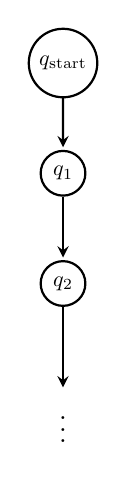
\begin{tikzpicture}[->,>=stealth,shorten >=1pt,auto,node distance=1.75cm,thick,main node/.style={scale=0.8,circle,draw,font=\sffamily\normalsize}]
                \node[main node] (1) {$q_\mathrm{start}$};
                \node[main node] (2) [below of=1] {$q_1$};
                \node[main node] (3) [below of=2] {$q_2$};
                \node[] (4) [below of=3] {$\vdots$};
    
                \path[every node/.style={font=\sffamily\small}]
                    (1) edge (2)
                    (2) edge (3)
                    (3) edge (4)
                    ;
            \end{tikzpicture}

            &\qquad\qquad\qquad&

            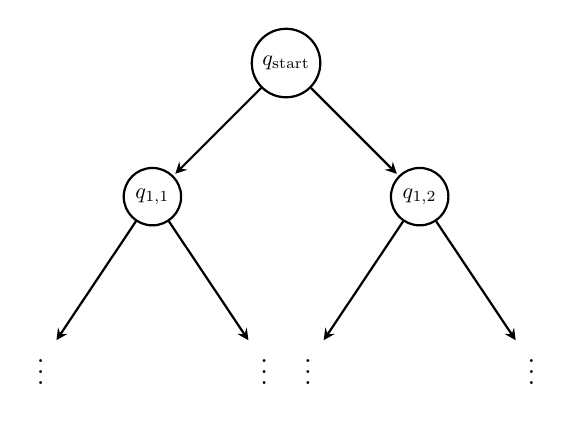
\begin{tikzpicture}[->,>=stealth,shorten >=1pt,auto,node distance=3cm,thick,main node/.style={scale=0.8,circle,draw,font=\sffamily\normalsize}]
                \node[main node] (1) {$q_\mathrm{start}$};
                \node[main node] (2) [below left of=1] {$q_{1,1}$};
                \node[main node] (3) [below right of=1] {$q_{1,2}$};
                \node[] (4) [below left of=2, xshift=20] {$\vdots$};
                \node[] (5) [below right of=2, xshift=-20] {$\vdots$};
                \node[] (6) [below left of=3, xshift=20] {$\vdots$};
                \node[] (7) [below right of=3, xshift=-20] {$\vdots$};

                \path[every node/.style={font=\sffamily\small}]
                    (1) edge (2)
                    (1) edge (3)
                    (2) edge (4)
                    (2) edge (5)
                    (3) edge (6)
                    (3) edge (7)
                    ;
            \end{tikzpicture}
        \end{tabular}

        \caption{A deterministic computation (left) and a non-deterministic one (right)}
    \end{figure}

    \begin{frameddefn}{The $\mathrm{NTIME}$ class}
        Given a function $T : \N \to \R^+$, we define $\mathrm{NTIME}(T(n))$ as the class of the languages of decision problems computable by a \textsf{NDTM} for which any input $x \in \{0,1\}^*$ of length $\abs{x} \leq n$ is accepted or refused in at most $O(T(n))$.
    \end{frameddefn}

    Surprisingly, the concept of efficient non-deterministic Turing machine is equivalent to the concept of efficient verification, meaning that \textsf{NP} is also the class of all the languages decidable in polynomial time by a \textsf{NDTM} \cite{cook_sat, karp}. In fact, this was the original definition of this class of decision problems, hence the name \textsf{NP} standing for Non-deterministic \textsf{P}. However, since non-deterministic Turing machines are only a theoretical tool and not a real, concrete and realizable model of computation, it was quickly changed to the one based on verification.

    \begin{framedthm}{The class $\mathsf{NP}$ (2nd Definition)}
        $\NPclass = \bigcup\limits_{k \geq 0} \mathrm{NTIME}(n^k)$
    \end{framedthm}

    \begin{proof}
        Suppose $L$ has a polynomial time verifier $V$ in time at most $n^k$, for some $k \in \N$. We know that for each input $x \in L$ there is a witness $w \in \{0,1\}^{n^k}$. We define a \textsf{NDTM} $N$ that takes in input the string $x$, non-deterministically generates all the possible strings $w \in \{0,1\}^{n^k}$ and then runs $V(x,w)$, accepting if and only if $V$ accepts. Each branch takes at most $2n^k$ steps.
        \[x \in L \iff \exists w \in \{0,1\}^* \;\;V(x,w) = 1 \iff \text{A branch of $N$ accepts}\]
        
        Now suppose that $L$ is decided by a \textsf{NDTM} $N'$ in time at most $n^k$, for some $k \in \N$. Then, we know that $\forall x \in L$ there is at least a path $P$ of length at most $n^k$ that accepts $x$. We define a verifier $V'$ for which the encoding of the accepting path of each input acts as the witness, concluding that:
        \[x \in L \iff \text{A path $P$ of $N'(x)$ accepts} \iff \exists \abk{P} \in \{0,1\}^* \;\; V'(x,P) = 1\]
        concluding that $L \in \textsf{NP}$. 
    \end{proof}

    \section{Reductions and \textsf{NP}-Completeness}

    One of the most interesting aspects of computable (and uncomputable) problems is the ability to be transformed into another problem in order to achieve a solution. Suppose that we have an instance $a$ of problem $A$ and that we know an algorithm that transforms $a$ into an instance $b$ of a problem $B$ such that $a$ is a \say{yes} answer if and only if $b$ is a \say{yes} answer. Then, by solving $b$ we would get an answer to $a$.
    
    In computer science, this concept is known as \textbf{reduction}: a problem $A$ is said to be reducible into a problem $B$, written as $A \leq B$, if any instance $a$ of $A$ can be mapped into an instance $b$ of $B$ whose solution gives a solution to the former. For instance, the proof of the uncomputability of $\mathrm{HALT}$ given for \Cref{halt}. In that case, we \textit{reduced} $\mathrm{UC}$ to $\mathrm{HALT}$.
    
    \textit{Many-to-one reductions} are the simplest type of reduction possible, where a function $f$ maps strings from a language $A$ to strings of a language $B$.

    \begin{frameddefn}{Many-to-one reduction}
        Given two languages $A, B$, we say that $A$ is \textbf{many-to-one reducible} to $B$, written as $A \leq_m B$, if there is a function $f : \{0,1\}^* \to \{0,1\}^*$ such that:
        \[x \in A \iff f(x) \in B\]
    \end{frameddefn}

    For example, consider the problems $\mathrm{3\text{-}SAT}$ and $\mathrm{SAT}$. The former is clearly reducible to the latter through the identity function $\mathrm{f}(x) = x$: a 3-CNF formula $F$ is satisfiable if and only if $F$ itself is satisfiable!.

    For example, consider the problems $\mathrm{CNF\text{-}SAT}$ and $\mathrm{3\text{-}SAT}$. We can construct a many-one-reduction from the former problem to the latter. Consider a CNF formula $F = \bigwedge_{i = 1}^m C_j$ where $C_j$ is a logical clause, i.e. $C_j = \bigvee_{i = 1}^{k_j} \ell_{i,j}$. We can construct a new 3-CNF formula $F' = \bigwedge_{i = 1}^m D_i$ by substituting each clause $C_i$ with a new subformula $D_i$:
    \begin{enumerate}
        \item If $C_j = \ell_{1,j}$, we set $D_j$ equal to:
        \[D_j = (\ell_{1,j} \lor y_{1,j} \lor y_{2,j})(\ell_{1,j} \lor \overline{y_{1,j}} \lor y_{2,j})(\ell_{1,j} \lor y_{1,j} \lor \overline{y_{2,j}})(\ell_{1,j} \lor \overline{y_{1,j}} \lor \overline{y_{2,j}})\]
        where $y_{1,j}, y_{2,j}$ are two new variables.

        
        \item If $C_j = \ell_{1,j} \lor \ell_{2,j}$, we set $D_j$ equal to:
        \[D_j = (\ell_{1,j} \lor \ell_{2,j} \lor y_{1,j})(\ell_{1,j} \lor \ell_{2,j} \lor \overline{y_{1,j}})\]
        where $y_{1,j}$ is a new variable.

        \item If $C_j = \ell_{1,j} \lor \ell_{1,j} \lor \ell_{3,j}$, we set $D_j = C_j$.
        \item If $C_j = \ell_{1,j} \lor \ldots \lor \ell_{k_j.j}$ with $k_j > 3$, we define $D_j$ as:
        \[D_j = (\ell_{1,j} \lor \ell_{2,j} \lor y_{1,j})(\overline{y_{1,j}} \lor \ell_{3,j} \lor y_{1,j}) \ldots (\overline{y_{k_j-3,j}} \lor \ell_{k_j-2, j} \lor y_{k_j-2,j})(\overline{y_{k_j-2,j}} \lor \ell_{k_j-1,j} \lor \ell_{k_j,j})\]
    \end{enumerate}

    For the first three cases, it's easy to see that given an assignment $\alpha$ it holds that $C_j(\alpha) = 1 \iff D_j(\alpha)$. The fourth case, instead, requires more attention. Suppose that there is an assignment $\alpha$ that satisfies $C_i$. This implies that at least one $\ell_{i,j}$ must be set to true in $\alpha$. Then, in every other subclause of $D_j$, we can set one between $y_{t,j}$ or $\overline{y_{t,j-1}}$ to true in order to satisfy $D_j$. Vice versa, suppose that there is an assignment $\beta$ that satisfies $D_j$. By way of contradiction, suppose that $\ell_{1,j}, \ldots, \ell_{k_j,j} = 0$ in $\beta$. Without loss of generality, we can assume that $y_{1,j}, \ldots, y_{k_j-3,j} = 1$ in $\beta$. Then, for any assignment of $y_{1,k_j-2}$, one between the clause $(\overline{y_{k_j-3,j}} \lor \ell_{k_j-2,j} \lor y_{k_j-2,j})$ or $(\overline{y_{k_j-2,j}} \lor \ell_{k_j-1,j} \lor \ell_{k_j,j})$ cannot be satisfiable, raising a contradiction. Thus, there must be at least one $\ell_{i,j}$ set to true in $\beta$, implying that $\beta$ also satisfies $C_j$.This concludes that $F$ is satisfiable if and only if $F'$ is satisfiable. Moreover, $F'$ is a 3-CNF, hence $\mathrm{CNF\text{-}SAT} \leq_m \mathrm{3\text{-}SAT}$.

    Many-to-one reductions between problems are transitive: starting from a problem $A$, we can reduce it to a problem $B$ through a function $f$ and then reduce it to a problem $C$ through a function $g$. This implies that $h = g \circ f$ is a reduction from $A$ to $C$. Hence, we have that $\mathrm{CNF\text{-}SAT} \leq_m \mathrm{3\text{-}SAT} \leq_m \mathrm{SAT}$.

    \begin{framedprop}{Transitive reduction}
        Given three languages $A, B, C$, if $A \leq_m B$ and $B \leq_m C$ then $A \leq_m C$.
    \end{framedprop}

    In particular, we notice that both of the previous reductions are easily computable in polynomial time by a Turing machine. When this happens, the reduction is said to be a \textbf{Karp reduction} \cite{karp}.

    \begin{frameddefn}{Karp reduction}
        Given two languages $A, B$, we say that $A$ is \textbf{Karp reducible} to $B$, written as $A \leq_P B$, if there is a many-to-one reduction from $A$ to $B$ computable in polynomial time
    \end{frameddefn}
    
    For instance, the previous reduction from $\mathrm{CNF\text{-}SAT}$ to $\mathrm{3\text{-}SAT}$ can actually be computed in polynomial time, hence $\mathrm{CNF\text{-}SAT} \leq_P \mathrm{3\text{-}SAT}$.    Clearly, transitivity between reductions also holds in this case: if two reductions $f$ and $g$ are both computable in polynomial time then $h = g \circ f$ also is.
    
    \begin{framedprop}{Transitive Karp reduction}
        Given three languages $A, B, C$, if $A \leq_P B$ and $B \leq_P C$ then $A \leq_P C$.
    \end{framedprop}

    When a problem $A$ is Karp reducible to a problem $B$ solvable (or verifiable) in polynomial time by a machine $M$, i.e. a problem that is in \Pclass (or \NPclass), we can build a new Turing machine $M'$ that first computes the reduction from $A$ to $B$, then runs $M$ and finally accepts if and only if $M$ accepts the reduced instance. This new machine $M'$ clearly also requires polynomial time, meaning that $A$ is also solvable (or verifiable) in polynomial time.

    \begin{framedprop}{}
        Let $A, B$ be two languages such that $A \leq_P B$. Then:
        \begin{itemize}
            \item If $B \in \Pclass$ then $A \in \Pclass$.
            \item If $B \in \NPclass$ then $A \in \NPclass$.
        \end{itemize}
    \end{framedprop}

    Reductions between problems enable us to \textit{classify} problems based on their \curlyquotes{hardness}: if a problem $A$ is efficiently reducible to a problem $B$, then solving $A$ cannot be harder than solving $B$, forming some sort of hierarchy between problems. In other words, if $A \leq_P B$ then $A$ is at most hard as $B$ and $B$ is at least as easy as $A$. 

    Building on this idea of hardness, we can identify some privileged problems that are harder than a whole class of problems! For example, every problem from the class \NPclass is efficiently reducible to a single problem $B$, then each \NPclass problem is as hard as $B$. When this happens, we say that $B$ is \textbf{\NPclass-Hard}. When an \NPclass-Hard problem also lies in \NPclass, we say that such problem is \textbf{\NPclass-Complete}.

    \begin{frameddefn}{\NPclass-Hardness and \NPclass-Completeness}
        A language $B$ is said to be \NPclass-Hard if $\forall A \in \NPclass$ it holds that $A \leq_P B$. If $B$ is also in \NPclass, we say that it is \NPclass-Complete.
    \end{frameddefn}

    The simplest \NPclass-Complete problem is the \textit{\TM satisfiability problem}, defined as:
    \[\mathrm{TM\text{-}SAT}(x) = \soe{ll}{
        1 & \text{if $x = \abk{\alpha, y,1^n, 1^t}$ and $\exists w \in \{0,1\}^n$ s.t. $M_\alpha(y,w) = 1$ within $t$ steps} \\
        0 & \text{otherwise}
    }\]

    First we show that this problem is in $\NPclass$. Given an input $x = \abk{\alpha, y,1^n, 1^t}$ and a witness $w \in \{0,1\}^*$, we start by asserting that $\abs{w} = n$. Then, we simulate $M_\alpha(y,w)$ with a counter that immediately stops if the simulation executes more than $t$ steps. Since the input has size $\abs{x} \geq t$ and the simulation takes at most $t$ steps, the verifier requires polynomial time, concluding that $\mathrm{TM\text{-}SAT} \in \NPclass$. Finally, we show that this problem is also \NPclass-Hard. Given a language $A \in \NPclass$, we know that it can be verified in at most $\abs{x}^k$ steps for some $k \in \N$. Suppose that such verifier is encoded by $\beta$. The reduction is easily given by mapping any input $x \in A$ to $f(x) = \abk{\beta, x, 1^{\abs{w}}, 1^{\abs{x}^k}}$, where $w$ is $x$'s witness for $A$, concluding that $A \leq_P \mathrm{TM\text{-}SAT}$.

    We notice that, by definition, \NPclass-Hard problems can even be uncomputable! For instance, consider the \textit{input acceptance problem}:
    \[\mathrm{ACCEPT}(x) = \soe{ll}{
        1 & \text{if $x = \abk{\alpha, y}$ and $M_\alpha(y) = 1$} \\
        0 & \text{otherwise} \\
    }\]

    It's pretty easy to see that any \NPclass problem (and more generally any computable problem) is Karp reducible to $\mathrm{ACCEPT}$, meaning that $\mathrm{ACCEPT}$ is \NPclass-Hard. However, this problem is clearly uncomputable since $\mathrm{HALT} \leq_m \mathrm{ACCEPT}$. 

    If an \NPclass-Hard problem could be solved in polynomial time, i.e. be inside \Pclass, then every single problem \NPclass-Hard problem would also be solvable in polynomial time, meaning that $\Pclass = \NPclass$. However, when an \NPclass-Hard problem also lies in the class \NPclass, this relation also becomes valid in the opposite direction: if $\Pclass = \NPclass$ then any \NPclass-Hard problem that is in \NPclass is also in \Pclass.

    \begin{framedprop}{}
        Given a language $B$, it holds that:
        \begin{itemize}
            \item If $B$ is \NPclass-Hard then $B \in \Pclass$ implies that $\Pclass = \NPclass$
            \item If $B$ is \NPclass-Complete then $B \in \Pclass$ if and only if $\Pclass = \NPclass$
        \end{itemize} 
    \end{framedprop}

    In other words, if an \NPclass-Complete problem is proven to be solvable or unsolvable in polynomial time, we would get a proof for the $\Pclass \stackrel{?}{=} \NPclass$ question. Moreover, by definition, each \NPclass-Complete is Karp reducible to one another, meaning that they all of them share the same hardness. These are the reasons why these problems are referred to as \textit{complete}. 

    Even though it is indeed \NPclass-Complete, the problem $\mathrm{TM\text{-}SAT}(x)$ is quite artificial since, by definition, in order to efficiently solve it we would have to be capable of efficiently solving any efficiently verifiable problem, which is literally the same as asking to solve the $\Pclass \stackrel{?}{=} \NPclass$ question. A more interesting \NPclass-Complete problem is the \textit{satisfiability problem} discussed in the previous sections, which actually is the first ever problem to be shown to be \NPclass-Complete. This result is known as the Cook-Levin theorem \cite{cook_sat, levin_fsat}.

    \begin{framedthm}[label={cook_levin}]{The Cook-Levin theorem}
        $\mathrm{SAT}$ and $\mathrm{3\text{-}SAT}$ are \NPclass-Complete
    \end{framedthm}

    The standard proof of this theorem is quite long and tedious, requiring a very careful notation in order to make things clearer. Instead, we will achieve this theorem by proving that the \textit{circuit satisfiability problem} is \NPclass-Complete and then reducing it to both $\mathrm{SAT}$ and $\mathrm{3\text{-}SAT}$. For the moment being, we will assume to have proved this theorem.

    \section{The Web of Reductions}

    The easiest way to show that a problem is \NPclass-Complete is to show that it lies inside \NPclass and then find a Karp-reduction from another \NPclass-Complete problem to it. Through this idea, we can form a \textit{web of reductions} between \NPclass-Complete problems. In fact, this was the original idea used by Karp \cite{karp} to prove his famous 21 \NPclass-Complete problems starting from the $\mathrm{SAT}$ problem (hence the name Karp reductions).
    
    \begin{figure}[H]
        \centering
        \includegraphics[scale=0.475]{images/karp.png}

        \caption{Karp's original 21 \NPclass-Complete problems reduction tree}
    \end{figure}

    Some problems can be shown to be \NPclass-Complete simply by being an extension of an already known \NPclass-Complete problem. For instance, we have shown that $\mathrm{CNF\text{-}SAT} \leq_P \mathrm{3\text{-}SAT}$, but the reverse also holds since the former is just an extension of the latter (the reduction is the identity function). Moreover, $\mathrm{CNF\text{-}SAT}$ is trivially in \textsf{NP}: the witness is the satisfying assignment. This concludes that $\mathrm{CNF\text{-}SAT}$ is also \NPclass-Complete.

    \begin{framedthm}{}
        $\mathrm{CNF\text{-}SAT}$ is \NPclass-Complete.
    \end{framedthm}

    Consider now the \textit{0/1 integer programming problem}:
    \[\mathrm{0/1\text{-}PROG}(x) = \soe{ll}{
        1 & \text{if $x = \abk{P}$ and $P$ is a feasible 0/1 program} \\
        0 & \text{otherwise}
    }\]

    An 0/1 integer program is a linear program defined on $n$ variables, $m$ inequalities, called constraints, and an objective function, where $x_1, \ldots, x_n \in \{0,1\}$. In a linear program, we want to find the optimal combination of the values of $x_1, \ldots, x_n$ that maximize the value of the objective function. A linear program is said to be feasible if there is at least one possible assignment for $x_1, \ldots, x_n$ that satisfies all the constraints.

    \begin{framedthm}[label=01_prog]{}
        $\mathrm{0/1\text{-}PROG}$ is \NPclass-Complete.
    \end{framedthm}

    \begin{proof}
        Here, the witness is nothing more than a feasible assignment for $x_1, \ldots, x_n$, which can be checked in polynomial time. Moreover, we can easily reduce $\mathrm{3\text{-}SAT}$ by expressing every clause inside a CNF formula as a sum between the three literals whose value must be at least 1. For example, the clause $(x_1 \lor \overline{x_2} \lor \overline{x_3})$ can be expressed as the constraint $x_1 + (1-x_2) + (1-x_3) \geq 1$. Clearly, each formula is satisfiable if and only if its corresponding linear program has a feasible solution.
    \end{proof}
    
    Now, we shift our focus to a more complex reduction. Consider the \textit{independent set problem}:
    \[\mathrm{IND\text{-}SET}(x) = \soe{ll}{
        1 & \text{if $x = \abk{G,k}$ and $G$ is a graph with an ind. set. $S$ such that $\abs{S} \geq k$} \\
        0 & \text{otherwise}
    }\]

    An independent set of a graph $G$ is a subset of vertices that share no edge between each other. Formally, $S \subseteq V(G)$ is an independent set of $G$ when $\forall u,v \in S$ it holds that neither $(u,v)$ nor $(v,u)$ is inside $E(G)$.
    
    \begin{framedthm}{}
        $\mathrm{IND\text{-}SET}$ is \NPclass-Complete.
    \end{framedthm}

    \begin{proof}
        For $\mathrm{IND\text{-}SET}$, the certifying witness is trivially an independent set of size $k$ inside $G$, which can be checked in linear time.

        Again, we can reduce $\mathrm{3}\text{-}SAT$ to this problem. However, this time we require a less immediate conversion. Consider a CNF formula $F = \bigwedge_{i = 1}^m C_i$ where $C_i$ is a logical clause with 3 literals. We construct a graph $G_F$ from $F$ as follows:
        \begin{enumerate}
            \item For each clause $C_i = (\ell_1 \lor \ell_2 \lor \ell_3)$, add three nodes $\ell_1, \ell_2, \ell_3$ (repeat the nodes if the same literal appears in more than a clause) and connect these three nodes by adding the edges $(\ell_1, \ell_2), (\ell_2, \ell_3) (\ell_3, \ell_1)$, forming a triangle
            \item For each node $\ell$ added in the previous step, add an edge between $\ell$ and every other node labeled with its negation, i.e. $\overline{\ell}$.
        \end{enumerate}

        Let $\alpha$ be an assignment of $F$. Without loss of generality, let $\ell_1^i$ be the literal that satisfies each clause $C_i$ (if there are more than one satisfying literal, just pick one of them). Let $S$ be a subset of vertices composed of each $\ell_1^i$ from each clause $C_i$. By construction, we know that $\ell_1^i$ is adjacent to $\ell_2^i, \ell_3^i$. Moreover, it is also adjacent to every other node labeled with its negation, that being the nodes $\overline{\ell_1^j}, \ldots, \overline{\ell_1^t}$.

        Suppose that $\alpha$ is a satisfying assignment for $F$. Since $\ell_1^i = 1$ inside $\alpha$, we know that $\overline{\ell_1^j}, \ldots, \overline{\ell_1^t} = 0$ inside $\alpha$. Since $S$ contains only $\ell_1^1, \ldots, \ell_1^m$, this is an independent set of size at least $m$ inside $G_F$.

        Vice versa, suppose that $\alpha$ doesn't satisfy $F$. This implies that at least one clause $C_j$ evaluates to 0, hence every literal inside it must be set to 0. This implies that $S$ has size less than $m$, hence its not an independent set of size at least $m$.

        We get that $F$ can be satisfiable if and only if there is an independent set of size at least $m$ inside $G_F$. Moreover, since each clause has a constant number of literals, this conversion can be built in polynomial time by a \TM, concluding that $\mathrm{3\text{-}SAT} \leq_P \mathrm{IND\text{-}SET}$.
    \end{proof}
    
    \begin{figure}[H]
        \centering
        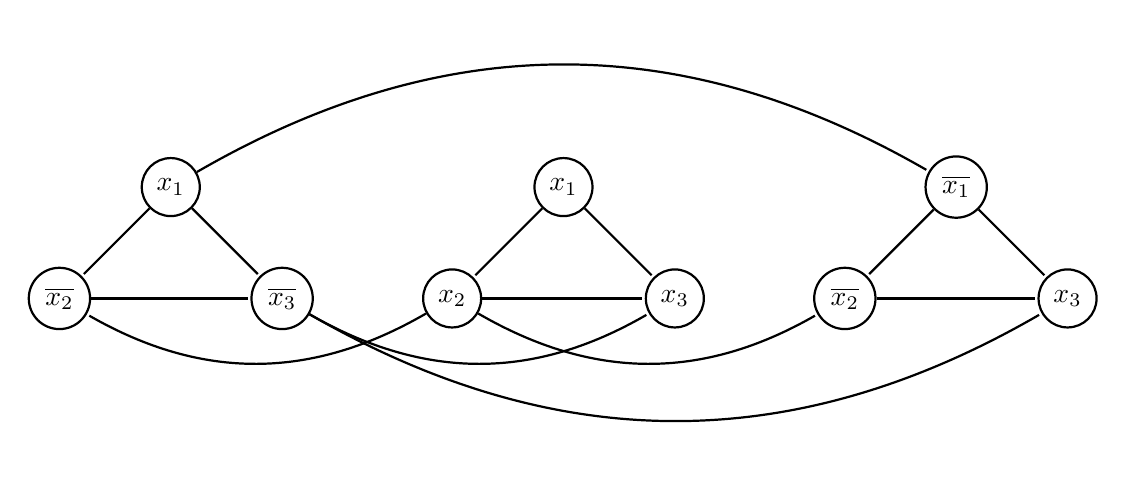
\begin{tikzpicture}[-,>=stealth,shorten >=1pt,auto,node distance=2cm,thick,main node/.style={scale=1,circle,draw,font=\sffamily\normalsize}]
            \node[main node] (1) []{$x_1$};
            \node[main node] (2) [below left of = 1]{$\overline{x_2}$};
            \node[main node] (3) [below right of = 1]{$\overline{x_3}$};

            \node[main node] (4) [right of = 1, xshift=85]{$x_1$};
            \node[main node] (5) [below left of = 4]{$x_2$};
            \node[main node] (6) [below right of = 4]{$x_3$};

            \node[main node] (7) [right of = 4, xshift=85]{$\overline{x_1}$};
            \node[main node] (8) [below left of = 7]{$\overline{x_2}$};
            \node[main node] (9) [below right of = 7]{$x_3$};

            \path[every node/.style={font=\sffamily\small}]
                (1) edge (2)
                (1) edge (3)
                (2) edge (3)

                (4) edge (5)
                (4) edge (6)
                (5) edge (6)

                (7) edge (8)
                (7) edge (9)
                (8) edge (9)

                (1) edge [bend left] (7)

                (5) edge [bend left] (2)
                (5) edge [bend right] (8)

                (3) edge [bend right] (6)
                (3) edge [bend right] (9)
            ;
        \end{tikzpicture}

        \caption{Conversion of the formula $(x_1 \lor \overline{x_2} \lor x_3)(x_1 \lor x_2 \lor x_3)(\overline{x_1} \lor \overline{x_2} \lor x_3)$}
    \end{figure}

    Once we have proven that the independent set problem is \textsf{NP}-Complete, we have a link between graph theory and complexity theory. This allows us to use the many known results in graph theory to easily extend our web of complete problems. For instance, consider the \textit{clique problem} and the \textit{vertex cover problem}:
    \[\mathrm{CLIQUE}(x) = \soe{ll}{
        1 & \text{if $x = \abk{G,k}$ and $G$ is a graph with a clique $C$ of size $\abs{C} \geq k$} \\
        0 & \text{otherwise}
    }\]
    \[\mathrm{V\text{-}COVER}(x) = \soe{ll}{
        1 & \text{if $x = \abk{G,k}$ and $G$ is a graph with a v. cov. $C$ of size $\abs{C} \leq k$} \\
        0 & \text{otherwise}
    }\]

    A clique of a graph $G$ is a subset of vertices all adjacent to each other. Formally, $C \subseteq V(G)$ is a clique of $G$ when $\forall u,v \in C$ it holds that $(u,v)$ or $(v,u)$ is inside $E(G)$. A vertex cover of a graph $G$, instead, is a subset of vertices capable of covering every edge of $G$. Formally, $V \subseteq V(G)$ is a vertex cover of $G$ when $\forall (u,v) \in E(G)$ it holds that either $u$ or $v$ is inside $V$.
    
    Like in $\mathrm{IND\text{-}SET}$, the certifying witness for $\mathrm{CLIQUE}$ and $\mathrm{V\text{-}COVER}$ are a clique and a vertex cover of size $k$ inside $G$. Two very standard results in graph theory state the following property, which descend directly from the definitions of independent set, clique and vertex cover.

    \begin{framedprop}{}
        Let $S \subseteq V(G)$ a subset of vertices of a graph $G$. Then, it holds that:
        \begin{enumerate}
            \item $S$ is an independent set of $G$ if and only if $S$ is a clique of $\overline{G}$
            \item $S$ is an independent set of $G$ if and only if $V(G)-S$ is a vertex cover of $G$
        \end{enumerate}

        \textit{Note}: $\overline{G}$ is the complementary graph of $G$, the graph with the same nodes of $G$ and all the opposite edges of $G$. Formally, $V(\overline{G}) = V(G)$ and $E(\overline{G}) = V(G) \times V(G) - E(G)$.
    \end{framedprop}

    This properties can be used to make two trivial reductions:
    \begin{enumerate}
        \item $\abk{G,k} \in \mathrm{IND\text{-}SET}$ if and only if $\abk{\overline{G},k} \in \mathrm{CLIQUE}$ 
        \item $\abk{G,k} \in \mathrm{IND\text{-}SET}$ if and only if $\abk{G,\abs{V(G)}-k} \in \mathrm{V\text{-}COVER}$ 
    \end{enumerate}
    which can both be built in polynomial time.

    \begin{framedthm}{}
        $\mathrm{CLIQUE}$ and $\mathrm{V\text{-}COVER}$ are \NPclass-Complete.
    \end{framedthm}

    Sometimes, graph properties aren't enough to establish a reduction from a graph problem to another. Case in point is the \textit{Hamiltonian path problem}. A Hamiltonian path on a graph $G$ is a path that traverses all the nodes of the graph. This problem is quite important in graph theory and it's part of the most studied ones.
    \[\mathrm{d\text{-}HAMPATH(x)} = \soe{ll}{
        1 & \text{if $x = \abk{G}$ and $G$ is a directed graph with a Hamiltonian path} \\
        0 & \text{otherwise}
    }\]

    This problem is also \textsf{NP}-Complete, however its proof is not so easy. First, we prove this for the directed version to then reduce it to the undirected case. It's easy to see that $\mathrm{d\text{-}HAMPATH(x)}$ is in \NPclass, since a Hamiltonian path can act as a witness. To show its completeness, we define a reduction from $\mathrm{3\text{-}SAT}$. Consider a CNF formula $F = \bigwedge_{i = 0}^{m-1} C_i$ where $C_i$ is a logical clause with 3 literals with a total of $n$ variables. We notice that the clauses of $F$ are numbered \underline{starting from 0} instead of 1. This will make the notation of the proof easier to read. 
    
    For each variable $x_i$, we construct a horizontal \curlyquotes{chain} of $6m$ vertices $v_{0}^i, \ldots, v_{6m-1}^i$. Each node inside the chain is bidirectionally adjacent to its near nodes. In other words, for each $j \in [0, 6m-2]$ we have that $(v^i_{j}, v^i_{j+1})$ and $(v^i_{j+1}, v^i_{j})$. The idea behind this chain of $6m$ vertices will be explained later in the proof.

    \begin{figure}[H]
        \centering
        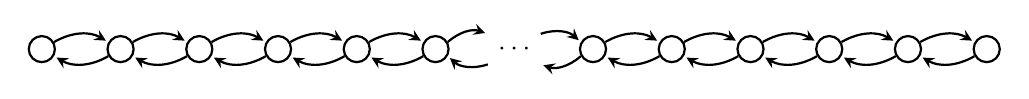
\begin{tikzpicture}[->,>=stealth,shorten >=1pt,auto,node distance=1cm,thick,main node/.style={scale=1,circle,draw,font=\sffamily\normalsize}]
            \node[main node] (1) []{};
            \node[main node] (2) [right of = 1]{};
            \node[main node] (3) [right of = 2]{};
            \node[main node] (4) [right of = 3]{};
            \node[main node] (5) [right of = 4]{};
            \node[main node] (6) [right of = 5]{};
            \node[] (7) [right of = 6]{$\cdots$};
            \node[main node] (8) [right of = 7]{};
            \node[main node] (9) [right of = 8]{};
            \node[main node] (10) [right of = 9]{};
            \node[main node] (11) [right of = 10]{};
            \node[main node] (12) [right of = 11]{};
            \node[main node] (13) [right of = 12]{};

            \path[every node/.style={font=\sffamily\small}]
            (1) edge[bend left] (2)
            (2) edge[bend left] (1)
            
            (2) edge[bend left] (3)
            (3) edge[bend left] (2)
            
            (3) edge[bend left] (4)
            (4) edge[bend left] (3)
            
            (4) edge[bend left] (5)
            (5) edge[bend left] (4)
            
            (5) edge[bend left] (6)
            (6) edge[bend left] (5)
            
            (6) edge[bend left] (7)
            (7) edge[bend left] (6)
            
            (7) edge[bend left] (8)
            (8) edge[bend left] (7)
            
            (8) edge[bend left] (9)
            (9) edge[bend left] (8)
            
            (9) edge[bend left] (10)
            (10) edge[bend left] (9)
            
            (10) edge[bend left] (11)
            (11) edge[bend left] (10)
            
            (11) edge[bend left] (12)
            (12) edge[bend left] (11)

            (12) edge[bend left] (13)
            (13) edge[bend left] (12)
            ;
        \end{tikzpicture}

        \caption{Horizontal chain of $6m$ vertices for a variable $x_i$}
    \end{figure}

    Then, we add $n+1$ more vertices $s_0, \ldots, s_{n}$ that connect these $n$ chains. The nodes $s_0, s_1, \ldots, s_{n-1}$ have two edges out-going to the extremes of their chain, i.e. $(s^i, v_1^i)$ and $(s^i, v_{6m-1}^i)$, and the nodes $s_1, \ldots, s_{n-1}, s_{n}$ have two in-going edges from the extremes of the previous chain, i.e. $(v_0^{i-1}, t^i)$ and $(v_{6m-1}^{i-1}, t^i)$. The final result is a sequence of diamond-shaped subgraphs.

    \begin{figure}[H]
        \centering
        \resizebox{0.8\hsize}{!}{
            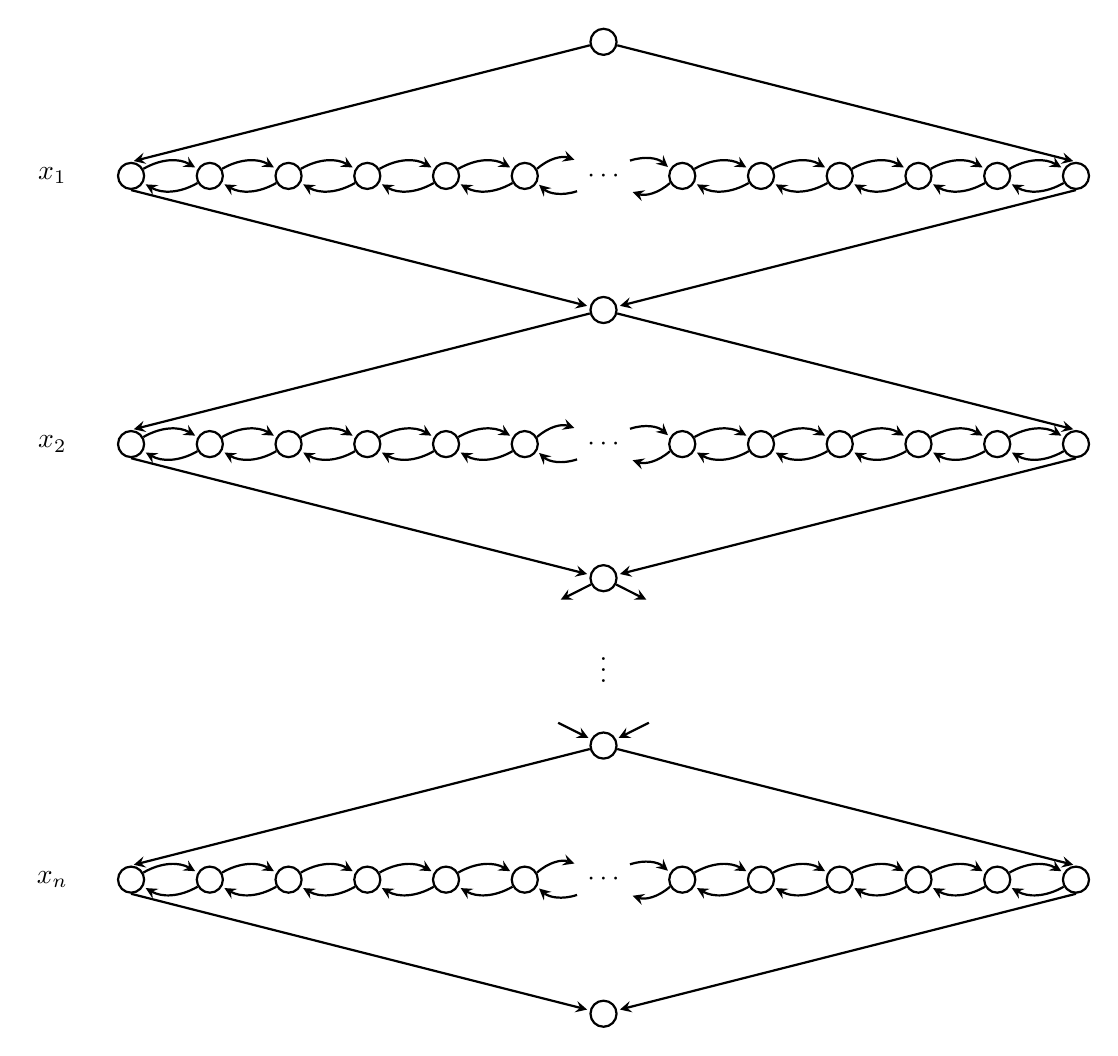
\begin{tikzpicture}[->,>=stealth,shorten >=1pt,auto,node distance=1cm,thick,main node/.style={scale=1,circle,draw,font=\sffamily\normalsize}]
                \node[main node] (1) []{};
                \node[main node] (2) [right of = 1]{};
                \node[main node] (3) [right of = 2]{};
                \node[main node] (4) [right of = 3]{};
                \node[main node] (5) [right of = 4]{};
                \node[main node] (6) [right of = 5]{};
                \node[] (7) [right of = 6]{$\cdots$};
                \node[main node] (8) [right of = 7]{};
                \node[main node] (9) [right of = 8]{};
                \node[main node] (10) [right of = 9]{};
                \node[main node] (11) [right of = 10]{};
                \node[main node] (12) [right of = 11]{};
                \node[main node] (13) [right of = 12]{};

                \node[main node] (14) [above of = 7, yshift=20]{};
                \node[main node] (15) [below of = 7, yshift=-20]{};

                \node[] (7b) [below of = 15, yshift=-20]{$\cdots$};
                \node[main node] (6b) [left of = 7b]{};
                \node[main node] (5b) [left of = 6b]{};
                \node[main node] (4b) [left of = 5b]{};
                \node[main node] (3b) [left of = 4b]{};
                \node[main node] (2b) [left of = 3b]{};
                \node[main node] (1b) [left of = 2b]{};
                \node[main node] (8b) [right of = 7b]{};
                \node[main node] (9b) [right of = 8b]{};
                \node[main node] (10b) [right of = 9b]{};
                \node[main node] (11b) [right of = 10b]{};
                \node[main node] (12b) [right of = 11b]{};
                \node[main node] (13b) [right of = 12b]{};

                \node[main node] (15b) [below of = 7b, yshift=-20]{};

                \node[] (x1) [below left of = 15b, yshift=10]{};
                \node[] (x2) [below right of = 15b, yshift=10]{};

                \node[] (x3) [below right of = x1]{$\vdots$};

                \node[] (x4) [below left of = x3]{};
                \node[] (x5) [below right of = x3]{};

                \node[main node] (14c) [below right of = x4, yshift=10]{};

                \node[] (7c) [below of = 14c, yshift=-20]{$\cdots$};
                \node[main node] (6c) [left of = 7c]{};
                \node[main node] (5c) [left of = 6c]{};
                \node[main node] (4c) [left of = 5c]{};
                \node[main node] (3c) [left of = 4c]{};
                \node[main node] (2c) [left of = 3c]{};
                \node[main node] (1c) [left of = 2c]{};
                \node[main node] (8c) [right of = 7c]{};
                \node[main node] (9c) [right of = 8c]{};
                \node[main node] (10c) [right of = 9c]{};
                \node[main node] (11c) [right of = 10c]{};
                \node[main node] (12c) [right of = 11c]{};
                \node[main node] (13c) [right of = 12c]{};

                \node[main node] (15c) [below of = 7c, yshift=-20]{};

                \node[] (z1) [left of = 1]{$x_1$};
                \node[] (z2) [left of = 1b]{$x_2$};
                \node[] (z3) [left of = 1c]{$x_n$};


                \path[every node/.style={font=\sffamily\small}]
                (1) edge[bend left] (2)
                (2) edge[bend left] (1)
                
                (2) edge[bend left] (3)
                (3) edge[bend left] (2)
                
                (3) edge[bend left] (4)
                (4) edge[bend left] (3)
                
                (4) edge[bend left] (5)
                (5) edge[bend left] (4)
                
                (5) edge[bend left] (6)
                (6) edge[bend left] (5)
                
                (6) edge[bend left] (7)
                (7) edge[bend left] (6)
                
                (7) edge[bend left] (8)
                (8) edge[bend left] (7)
                
                (8) edge[bend left] (9)
                (9) edge[bend left] (8)
                
                (9) edge[bend left] (10)
                (10) edge[bend left] (9)
                
                (10) edge[bend left] (11)
                (11) edge[bend left] (10)
                
                (11) edge[bend left] (12)
                (12) edge[bend left] (11)

                (12) edge[bend left] (13)
                (13) edge[bend left] (12)

                (14) edge (1.north)
                (14) edge (13.north)

                (1.south) edge (15)
                (13.south) edge (15)

                (1b) edge[bend left] (2b)
                (2b) edge[bend left] (1b)
                
                (2b) edge[bend left] (3b)
                (3b) edge[bend left] (2b)
                
                (3b) edge[bend left] (4b)
                (4b) edge[bend left] (3b)
                
                (4b) edge[bend left] (5b)
                (5b) edge[bend left] (4b)
                
                (5b) edge[bend left] (6b)
                (6b) edge[bend left] (5b)
                
                (6b) edge[bend left] (7b)
                (7b) edge[bend left] (6b)
                
                (7b) edge[bend left] (8b)
                (8b) edge[bend left] (7b)
                
                (8b) edge[bend left] (9b)
                (9b) edge[bend left] (8b)
                
                (9b) edge[bend left] (10b)
                (10b) edge[bend left] (9b)
                
                (10b) edge[bend left] (11b)
                (11b) edge[bend left] (10b)
                
                (11b) edge[bend left] (12b)
                (12b) edge[bend left] (11b)

                (12b) edge[bend left] (13b)
                (13b) edge[bend left] (12b)

                (15) edge (1b.north)
                (15) edge (13b.north)

                (1b.south) edge (15b)
                (13b.south) edge (15b)

                (15b) edge (x1)
                (15b) edge (x2)

                (x4) edge (14c)
                (x5) edge (14c)

                (1c) edge[bend left] (2c)
                (2c) edge[bend left] (1c)
                
                (2c) edge[bend left] (3c)
                (3c) edge[bend left] (2c)
                
                (3c) edge[bend left] (4c)
                (4c) edge[bend left] (3c)
                
                (4c) edge[bend left] (5c)
                (5c) edge[bend left] (4c)
                
                (5c) edge[bend left] (6c)
                (6c) edge[bend left] (5c)
                
                (6c) edge[bend left] (7c)
                (7c) edge[bend left] (6c)
                
                (7c) edge[bend left] (8c)
                (8c) edge[bend left] (7c)
                
                (8c) edge[bend left] (9c)
                (9c) edge[bend left] (8c)
                
                (9c) edge[bend left] (10c)
                (10c) edge[bend left] (9c)
                
                (10c) edge[bend left] (11c)
                (11c) edge[bend left] (10c)
                
                (11c) edge[bend left] (12c)
                (12c) edge[bend left] (11c)

                (12c) edge[bend left] (13c)
                (13c) edge[bend left] (12c)

                (14c) edge (1c.north)
                (14c) edge (13c.north)

                (1c.south) edge (15c)
                (13c.south) edge (15c)
                ;
            \end{tikzpicture}
        }

        \caption{Sequence of diamond-shaped subgraphs for the formula $F$}
    \end{figure}

    Let's discuss what we have constructed until now. Consider a Hamiltonian path that starts from $s_0$ and ends on $s_{n}$. On the first edge, this path has to take either the left or the right edge out-going from $s_0$. Without loss of generality, suppose that it takes the edge on the left. Then, this path has to traverse the whole chain of $x_0$ from left to right and then go to the node $s_1$. The same argument holds for all the other chain-connecting nodes.
    
    Hence, this graph contains exactly $2^n$ Hamiltonian paths. Now, we will assume that when the chain $i$ is traversed by a path \textit{from left to right} then the variable $x_i$ will be considered as set to \textit{true}, while when the path traverses it \textit{from right to left} we will assume that $x_i$ is \textit{false}. With this idea in mind, we get a perfect bijection from each Hamiltonian path to each possible assignment of $F$.

    However, this means that each formula with $n$ variables and $6m$ clauses will produce the same graph. To distinguish between each formula, we have to introduce some \curlyquotes{gadgets} that model the clauses of $F$.

    First, we introduce $m$ nodes $c_0, \ldots, c_{m-1}$, each corresponding to a clause of $F$. The idea here is that the first 6 nodes of the chain $i$ will be reserved for possible connections to the clause $C_0$, while the next 6 nodes will be reserved for connections to the clause $C_1$ and so on. Thus, each chain is partitioned into 6 subchains, one for each clause. Moreover, each of these subchains is again partitioned into 3 pairs of adjacent nodes used to describe if the $x_i$ variable or its negation $\overline{x_i}$ is inside $C_i$ and in what position. 
    
    Formally, consider a clause $C_j = \ell_0 \lor \ell_1 \lor \ell_2$. When the literal $\ell_t$ of such clause $C_j$ corresponds to the variable $x_i$, we add the edges $(v^i_{6j+2t}, c_j), (c_j, v^i_{6j+2t+1})$. Instead, when the literal $\ell_t$ of such clause $C_j$ corresponds to the negation $\overline{x_i}$ of a variable, we add the edges $(v^i_{6j+2t+1}, c_j), (c_j, v^i_{6j+2t})$. In other words, if $\ell = x_i$ then we force the direction $v^i_{6j+2t} \to c_j \to v^i_{6j+2t+1}$ on the path, while if $\ell = \overline{x_i}$ then we force the reverse direction $v^i_{6j+2t+1} \to c_j \to v^i_{6j+2t}$ on the path.


    \begin{figure}[H]
        \centering
        \resizebox{1\hsize}{!}{
            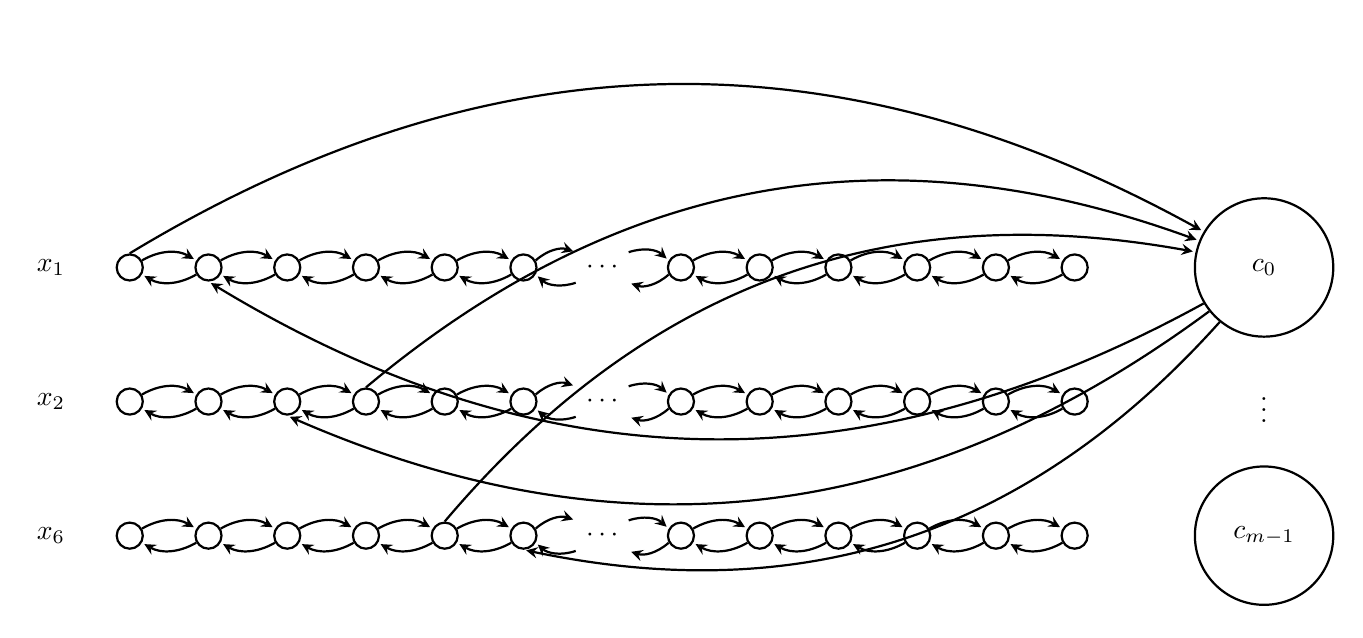
\begin{tikzpicture}[->,>=stealth,shorten >=1pt,auto,node distance=1cm,thick,main node/.style={scale=1,circle,draw,font=\sffamily\normalsize}]
                \node[main node] (1) []{};
                \node[main node] (2) [right of = 1]{};
                \node[main node] (3) [right of = 2]{};
                \node[main node] (4) [right of = 3]{};
                \node[main node] (5) [right of = 4]{};
                \node[main node] (6) [right of = 5]{};
                \node[] (7) [right of = 6]{$\cdots$};
                \node[main node] (8) [right of = 7]{};
                \node[main node] (9) [right of = 8]{};
                \node[main node] (10) [right of = 9]{};
                \node[main node] (11) [right of = 10]{};
                \node[main node] (12) [right of = 11]{};
                \node[main node] (13) [right of = 12]{};

                \node[] (7b) [below of = 7, yshift=-20]{$\cdots$};
                \node[main node] (6b) [left of = 7b]{};
                \node[main node] (5b) [left of = 6b]{};
                \node[main node] (4b) [left of = 5b]{};
                \node[main node] (3b) [left of = 4b]{};
                \node[main node] (2b) [left of = 3b]{};
                \node[main node] (1b) [left of = 2b]{};
                \node[main node] (8b) [right of = 7b]{};
                \node[main node] (9b) [right of = 8b]{};
                \node[main node] (10b) [right of = 9b]{};
                \node[main node] (11b) [right of = 10b]{};
                \node[main node] (12b) [right of = 11b]{};
                \node[main node] (13b) [right of = 12b]{};

                \node[] (7c) [below of = 7b, yshift=-20]{$\cdots$};
                \node[main node] (6c) [left of = 7c]{};
                \node[main node] (5c) [left of = 6c]{};
                \node[main node] (4c) [left of = 5c]{};
                \node[main node] (3c) [left of = 4c]{};
                \node[main node] (2c) [left of = 3c]{};
                \node[main node] (1c) [left of = 2c]{};
                \node[main node] (8c) [right of = 7c]{};
                \node[main node] (9c) [right of = 8c]{};
                \node[main node] (10c) [right of = 9c]{};
                \node[main node] (11c) [right of = 10c]{};
                \node[main node] (12c) [right of = 11c]{};
                \node[main node] (13c) [right of = 12c]{};

                \node[] (z1) [left of = 1]{$x_1$};
                \node[] (z2) [left of = 1b]{$x_2$};
                \node[] (z3) [left of = 1c]{$x_6$};

                \node[circle, draw, minimum size=50] (t1) [right of = 13, xshift=40]{$c_0$};
                \node[] (t2) [right of = 13b, xshift=40]{$\vdots$};
                \node[circle, draw, minimum size=50] (t3) [right of = 13c, xshift=40]{$c_{m-1}$};

                \path[every node/.style={font=\sffamily\small}]
                (1) edge[bend left] (2)
                (2) edge[bend left] (1)
                
                (2) edge[bend left] (3)
                (3) edge[bend left] (2)
                
                (3) edge[bend left] (4)
                (4) edge[bend left] (3)
                
                (4) edge[bend left] (5)
                (5) edge[bend left] (4)
                
                (5) edge[bend left] (6)
                (6) edge[bend left] (5)
                
                (6) edge[bend left] (7)
                (7) edge[bend left] (6)
                
                (7) edge[bend left] (8)
                (8) edge[bend left] (7)
                
                (8) edge[bend left] (9)
                (9) edge[bend left] (8)
                
                (9) edge[bend left] (10)
                (10) edge[bend left] (9)
                
                (10) edge[bend left] (11)
                (11) edge[bend left] (10)
                
                (11) edge[bend left] (12)
                (12) edge[bend left] (11)

                (12) edge[bend left] (13)
                (13) edge[bend left] (12)

                (1b) edge[bend left] (2b)
                (2b) edge[bend left] (1b)
                
                (2b) edge[bend left] (3b)
                (3b) edge[bend left] (2b)
                
                (3b) edge[bend left] (4b)
                (4b) edge[bend left] (3b)
                
                (4b) edge[bend left] (5b)
                (5b) edge[bend left] (4b)
                
                (5b) edge[bend left] (6b)
                (6b) edge[bend left] (5b)
                
                (6b) edge[bend left] (7b)
                (7b) edge[bend left] (6b)
                
                (7b) edge[bend left] (8b)
                (8b) edge[bend left] (7b)
                
                (8b) edge[bend left] (9b)
                (9b) edge[bend left] (8b)
                
                (9b) edge[bend left] (10b)
                (10b) edge[bend left] (9b)
                
                (10b) edge[bend left] (11b)
                (11b) edge[bend left] (10b)
                
                (11b) edge[bend left] (12b)
                (12b) edge[bend left] (11b)

                (12b) edge[bend left] (13b)
                (13b) edge[bend left] (12b)

                (1c) edge[bend left] (2c)
                (2c) edge[bend left] (1c)
                
                (2c) edge[bend left] (3c)
                (3c) edge[bend left] (2c)
                
                (3c) edge[bend left] (4c)
                (4c) edge[bend left] (3c)
                
                (4c) edge[bend left] (5c)
                (5c) edge[bend left] (4c)
                
                (5c) edge[bend left] (6c)
                (6c) edge[bend left] (5c)
                
                (6c) edge[bend left] (7c)
                (7c) edge[bend left] (6c)
                
                (7c) edge[bend left] (8c)
                (8c) edge[bend left] (7c)
                
                (8c) edge[bend left] (9c)
                (9c) edge[bend left] (8c)
                
                (9c) edge[bend left] (10c)
                (10c) edge[bend left] (9c)
                
                (10c) edge[bend left] (11c)
                (11c) edge[bend left] (10c)
                
                (11c) edge[bend left] (12c)
                (12c) edge[bend left] (11c)

                (12c) edge[bend left] (13c)
                (13c) edge[bend left] (12c)
                
                (1.north) edge[bend left] (t1)
                (t1) edge[bend left] (2.south)

                (4b.north) edge[bend left] (t1)
                (t1) edge[bend left] (3b.south)

                (5c.north) edge[bend left] (t1)
                (t1) edge[bend left] (6c.south)
                ;
            \end{tikzpicture}
        }

        \caption{Example of path restriction given by $C_0 = (x_1 \lor \overline{x_2} \lor x_6)$}
    \end{figure}

    Consider now an assignment $\alpha$ that satisfies $F$. We construct a path $P$ that traverses each chain $i$ from left to right if $\alpha(x_i) = 1$ and from right to left if $\alpha(x_i) = 0$. While traversing a chain, if the literal $\ell_t$ is the one that satisfies the clause $C_i$, the path also traverses the node $c_i$ through the two vertices reserved for that literal (choose only one if there is more than one satisfying literal). This path traverses all the nodes of the graph, concluding that $P$ is a Hamiltonian path of $G_F$.

    Vice versa, suppose that $G_F$ has a Hamiltonian path $P'$. We construct an assignment $\alpha'$ where the truthfulness of the variable $x_i$ depends on the direction which $P'$ traverses for the $i$-th chain. This assignment clearly satisfies $F$ since each clause $C_i$ will have to be traversed by at least one literal in order for $P'$ to be Hamiltonian.

    We conclude that $F$ is satisfiable if and only if $G_F$ has a Hamiltonian path. Since $G_F$ is a huge graph by construction, we have to check that we can build it in polynomial time. Each chain contains $6m$ nodes and $2(6m-1)$ edges, for a total of $6mn$ vertices and $2n(6m-1)$ edges. The we also have $n$ chain-connecting nodes, each with at most $2$ out-going and $2$ in-going edges, for a total of $n$ vertices and at most $4n$ edges. Finally, we have $m$ clause nodes, each with $6$ edges, for a total of $m$ more vertices and $6m$ more edges.
    
    Summing all of these values, we conclude that $G_F$ has a total of $6mn+n+m$ nodes and at most $2(6m-1) + 4n + 6m$ edges. This means that the reduction can indeed be built in polynomial time, concluding that $\mathrm{3\text{-}SAT} \leq_P \mathrm{d\text{-}HAMPATH}$.

    \begin{framedthm}{}
        $\mathrm{d\text{-}HAMPATH}$ is \NPclass-Complete.
    \end{framedthm}

    Once we have proved this result, we can extend it to other kinds of graph problems related to Hamiltonian paths, such as the undirected version of the \textit{Hamiltonian path problem} and the \textit{Hamiltonian cycle problem}, both directed and undirected. Here, a cycle is said to be Hamiltonian if it traverses each node only once, exception made for the first and last node of the cycle. These problems can be easily shown to be \NPclass-Complete by reducing $\mathrm{d\text{-}HAMPATH}$ to them.
    
    \begin{framedthm}{}
        $\mathrm{u\text{-}HAMPATH}, \mathrm{d\text{-}HAMCYCLE}$ and $\mathrm{u\text{-}HAMCYCLE}$ are \NPclass-Complete.
    \end{framedthm}

    To summarize, we have shown that, under the assumption that \nameref{cook_levin} is true, which states that $\mathrm{SAT}$ and $\mathrm{3\text{-}SAT}$ are \NPclass-Complete, the problems $\mathrm{CNF\text{-}SAT},$ $\mathrm{0/1\text{-}PROG}, \mathrm{IND\text{-}SET}, \mathrm{CLIQUE}, \mathrm{V\text{-}COVER}, \mathrm{u\text{-}HAMPATH}, \mathrm{d\text{-}HAMCYCLE}$ and \\$\mathrm{u\text{-}HAMCYCLE}$ are all \NPclass-Complete.

    Thousands of $\mathsf{NP}$ problems have been proven to be $\mathsf{NP}$-Complete, but none of them has been proven to be inside or outside of $\mathsf{P}$. Proving one of the two results would answer the $\mathsf{P} \stackrel{?}{=} \mathsf{NP}$ answer. The fact that we are incapable of efficiently solving any of these problems gives enough insight for modern researchers to believe that the answer to the conjecture is negative, i.e. $\mathsf{P} \neq \mathsf{NP}$. Moreover, some of these problems have also been proven to be \textbf{unapproximable} under a certain ratio. In the following sections and chapters, we will provide more results that make us believe that $\mathsf{P} \neq \mathsf{NP}$ must hold, since otherwise most \curlyquotes{\textit{obvious}} things in complexity theory would actually collapse.

    \newpage

    \section{The classes \textsf{EXP}, \textsf{NEXP}}

    We have seen how for some problems we still don't know if they lie only inside \textsf{NP} or if they also lie in \textsf{P}. However, we do know that some decision problem are strictly outside of \textsf{P}. For instance, consider the following variant of the halting problem:
    \[\mathrm{k\text{-}HALT}(x) = \soe{ll}{
        1 & \text{if $x = \abk{\alpha, y, k}$ and $M_\alpha(y)$ halts in at most $k$ steps} \\
        0 & \text{otherwise}
    }\]

    This problem strictly requires exponential time to be solved: the input value $k$ is encoded by $c \log k$ bits but the problem has to simulate $M_{\alpha}(y)$ for at least $k$ steps, which is exponential in terms of the input size. This means that $\mathrm{k\text{-}HALT} \notin \mathsf{P}$.

    We define the \textit{exponential versions} of the classes \textsf{P} and \textsf{NP} by relaxing the time constraint to being exponential with respect to the input.
    
    \begin{frameddefn}{The classes $\mathsf{EXP}$ and $\mathsf{NEXP}$}
        We define $\mathsf{EXP}$ as the class of the languages decidable in exponential time by a deterministic Turing machine as follows:
        \[\mathsf{EXP} = \bigcup_{k \geq 0} \mathrm{DTIME}(2^{n^k})\]
        Likewise, we define $\mathsf{NEXP}$ as the class of the languages decidable in exponential time by a non-deterministic Turing machine as follows:
        \[\mathsf{NEXP} = \bigcup_{k \geq 0} \mathrm{NTIME}(2^{n^k})\]

        \textit{Note}: we can also define \textsf{NEXP} through exponential time verifiers
    \end{frameddefn}

    From \Cref{np_exp}, we easily get that any problem that is verifiable in polynomial time can be decided in exponential time by a deterministic \TM. Moreover, like in the polynomial case, any deterministic exponential time Turing machine can be simulated by a non-deterministic Turing machine that has two exactly equal transition functions, requiring the same amount of time.

    \begin{framedprop}{}
        $\mathsf{P} \subseteq \mathsf{NP} \subseteq \mathsf{EXP} \subseteq \mathsf{NEXP}$
    \end{framedprop}

    Moreover, we know that $\mathrm{k\text{-}HALT} \notin \mathsf{P}$ but it clearly holds that $\mathrm{k\text{-}HALT} \in \mathsf{EXP}$. In the same fashion, we can define a very artificial problem that cannot be in \textsf{NP} but that definitely is inside \textsf{NEXP}.
    
    \begin{framedprop}{}
        $\mathsf{P} \subsetneq \mathsf{EXP}$ and $\mathsf{NP} \subsetneq \mathsf{NEXP}$.
    \end{framedprop}

    These results give us some insight on the \textsf{P} vs. \textsf{NP} question. In particular, since $\mathsf{P} \subsetneq \mathsf{EXP}$, we have only three possible alternatives for the decision hierarchy:
    \begin{enumerate}
        \item Each level is separated, meaning that $\mathsf{P} \subsetneq \mathsf{NP} \subsetneq \mathsf{EXP}$
        \item The separation lies only between $\mathsf{P}$ and $\mathsf{NP}$, meaning that $\mathsf{P} \subsetneq \mathsf{NP} = \mathsf{EXP}$
        \item The separation lies only between $\mathsf{NP}$ and $\mathsf{EXP}$, meaning that $\mathsf{P} = \mathsf{NP} \subsetneq \mathsf{EXP}$
    \end{enumerate}

    Furthermore, the \textsf{P} vs. \textsf{NP} question also translates to the exponential time world: we do not know whether $\mathsf{EXP} = \mathsf{NEXP}$ or not. However, we have an interesting correlation between the two questions:

    \begin{framedthm}{}
        If $\mathsf{EXP} \neq \mathsf{NEXP}$ then $\mathsf{P} \neq \mathsf{NP}$
    \end{framedthm}

    \begin{proof}
        We prove the contrapositive statement. We already know that $\mathsf{EXP} \subseteq \mathsf{NEXP}$ holds by definition, so we have to only show that if  $\mathsf{P} = \mathsf{NP}$ then $\mathsf{NEXP} \subseteq \mathsf{EXP}$ also holds.

        Given a language $L \in \mathsf{NEXP}$, let $L_{\mathrm{pad}}$ be the language defined as $L_{\mathrm{pad}} = \{x1^{2^{\abs{x}^k}} \mid x \in L\}$, where $k$ is some pre-fixed sufficiently large constant. The idea behind this theorem is to basically cheat by abusing definitions: since the running time of a machine is defined with respect to its input size, if we make the input size extremely large then the execution time will be \curlyquotes{efficient} with respect to the input size.

        Let $M$ be the machine that verifies $L$ in exponential time. Then, we define the machine $M'$ as follows:

        $M'$ = "Given the input strings $x$ and $w$:
        \begin{enumerate}
            \item Check that $x = \abk{y1^{2^{\abs{y}^k}}}$. If false, reject.
            \item Return $M(y,w)$."
        \end{enumerate}

        This machine clearly verifies $L_{\mathrm{pad}}$. Moreover, since the input size already is exponential, the execution of $M'$ will always run in polynomial time with respect to the input. Hence, we get that $L_{\mathrm{pad}} \in \mathsf{NP}$. Then, since $\mathsf{P} = \mathsf{NP}$ by assumption, we get that $L_{\mathrm{pad}} \in \mathsf{P}$. Through a machine $M''$ that decides $L_{\mathrm{pad}}$ in polynomial time, we can define another machine $M'''$ that decides $L$ in exponential time by bloating the input with an exponential number of ones and then running $M''$ on that input, concluding that $L \in \mathsf{EXP}$.
    \end{proof}
    
    The argument used in this theorem is usually called \textbf{time padding argument}. Even though this result is indeed interesting, finding a separation between $\mathsf{EXP}$ and $\mathsf{NEXP}$ is clearly more difficult than finding one for $\mathsf{P}$ and $\mathsf{NP}$: when we allow the time to be exponential, we can solve virtually any \curlyquotes{non-artificial} problem.

    \newpage

    \section{Disqualification, duality and the class \textsf{coNP}}

    We saw how $\mathrm{SAT}$ lies inside $\mathsf{NP}$ and how it actually is $\mathsf{NP}$-Complete. What can we say about his complementary language, i.e. $\overline{\mathrm{SAT}} = \{x \in \{0,1\}^* \mid x \notin \mathrm{SAT}\}$ ? We seem to not be able to show that this language is inside $\mathsf{NP}$: in order to \textit{verify} that a string lies in $\overline{\mathrm{SAT}}$, we would have to find a way to certify that this string is \textit{not} inside $\mathrm{SAT}$, which means that every possible witness cannot certify the membership of this string in $\mathrm{SAT}$. We define the class of all such languages as $\mathsf{coNP}$.

    \begin{frameddefn}{The class $\mathsf{coNP}$}
        We define $\mathsf{coNP}$ as the class of languages whose complement is in $\mathsf{NP}$:
        \[\mathsf{coNP} = \{L \subseteq \{0,1\}^* \mid \overline{L} \in \mathsf{NP}\}\]  
    \end{frameddefn}

    We observe that, by definition, the class $\mathrm{coNP}$ \textbf{is not equal to} $\overline{\mathsf{NP}}$, as the latter is the class of languages that aren't in $\mathsf{NP}$. Here, the prefix \curlyquotes{co} stands for \textit{dual} and \textbf{not for \textit{complement}}. Moreover, the concept of complementary language is different from the concept of \textbf{opposite} language: the opposite of a problem is the problem that asks the opposite question of the former (this doesn't imply that the answer to the latter is always the opposite of the former). For instance, consider the following problems:
    \[\mathrm{SAT} = \{\abk{\phi} \mid \phi \text{ is a CNF formula and } \exists \alpha \;\; \phi(\alpha) = 1\}\]
    \[\mathrm{UNSAT} = \{\abk{\phi} \mid \phi \text{ is a CNF formula and } \forall \alpha \;\; \phi(\alpha) = 0\}\]
    
    These two problems are opposites. By definition we have that $\mathrm{UNSAT} \subsetneq \overline{SAT}$: the language $\overline{\mathrm{SAT}}$ doesn't only contain CNF formulas that are unsatisfiable, but also gibberish strings in $\{0,1\}^*$ that aren't even encodings of CNF formulas! Nonetheless, the language $\mathrm{UNSAT}$ does still lie inside $\mathsf{coNP}$ since the language $\overline{\mathrm{UNSAT}}$ -- which is not equal to $\mathrm{SAT}$ -- can be easily verified in polynomial time. First, we check if the input string is a valid formula or not. If it is, the witness for its membership in $\overline{\mathrm{UNSAT}}$ is a satisfying assignment. Otherwise, if the string is gibberish, the witness can be any string.
    
    The $\mathsf{coNP}$ class can also be viewed from another more interesting prospective. Consider again the language $\mathrm{UNSAT}$. We know that $\overline{\mathrm{UNSAT}}$ has a polynomial time verifier $V$ such that:
    \[x \in \overline{\mathrm{UNSAT}} \iff \exists w \in \{0,1\}^{*} \; V(x,w) = 1\]

    By flipping this statement, we get that:
    \[x \notin \overline{\mathrm{UNSAT}} \iff \forall w \in \{0,1\}^{*} \; V(x,w) = 0\]

    Let $D$ be the two-input \TM defined as $D(x,w) = 1- V(x,w)$ -- in other words, $D$ returns the opposite of $V$'s result. Then, we have that:
    \[x \in \mathrm{UNSAT} \iff x \notin \overline{\mathrm{UNSAT}} \iff \forall w \in \{0,1\}^{*} \; D(x,w) = 1\]

    We get that the machine $D$ is a polynomial time \textbf{disqualifier} for $\mathrm{UNSAT}$: it is a machine that can prove that an input string \textit{doesn't} belong inside $\overline{\mathrm{UNSAT}}$, which in turn means that it lies inside $\mathrm{UNSAT}$. In other words, a disqualifier for a language is a machine capable of \curlyquotes{disqualifying} any witness that is trying to certify that the input belongs to the complement of the language -- think of this situation as if the disqualifier is fighting against an evil entity that is trying to prove that something is false. The class $\mathsf{coNP}$ can also be defined as the class of languages that can be disqualified in polynomial time.

    \begin{framedthm}{The class $\mathsf{coNP}$ (2nd Definition)}
        Given a language $L$, it holds that $L \in \mathsf{coNP}$ if and only if there is a polynomial time \TM $M$ such that: 
        \[x \in L \iff \forall w \in \{0,1\}^* \; M(x,w) = 1\]
    \end{framedthm}

    This new definition of $\mathsf{coNP}$ opens the doors to the concept of \textbf{duality}: to the property of two objects of being \curlyquotes{two faces of the same medal}. For example, consider the two following languages
    \[\mathrm{SAT} = \{\abk{\phi} \mid \phi \text{ is a CNF formula and } \exists \alpha \;\; \phi(\alpha) = 1\}\]
    \[\mathrm{TAUT} = \{\abk{\phi} \mid \phi \text{ is a DNF formula and } \forall \alpha \;\; \phi(\alpha) = 1\}\]

    These two languages are dual to each other: the concepts of CNF and DNF formulas are two faces of the same medal and the same goes for the quantifiers $\exists$ and $\forall$. Through the new definition, we can easily show that $\mathrm{TAUT}$ lies inside $\mathsf{coNP}$: if the given witness is a gibberish string then we accept, while if the given witness encodes an assignment then we accept if and only if it satisfies the input formula. When $\phi$ is a tautology, we know that all the possible assignments must satisfy it. Hence, if the input is a tautology, our machine is capable of disqualifying any witness that is trying to prove that $\phi$ is \textit{not} tautology, i.e. that it belongs to $\overline{\mathrm{TAUT}}$, meaning that it must indeed be a tautology.

    Duality and complementariness are two distinct concepts. For instance, $\mathrm{TAUT}$ is the dual problem of $\mathrm{SAT}$, but $\mathrm{TAUT}$ and $\overline{\mathrm{SAT}}$ are two totally different problems. Likewise, the concepts of duality and opposites are also distinct from each other. The dual of the $\mathrm{UNSAT}$ problem can be defined as:
    \[\mathrm{coUNSAT} = \{\abk{\phi} \mid \phi \text{ is a DNF formula and } \exists \alpha \;\; \phi(\alpha) = 0\}\]

    which, curiously, turns out to be the opposite of the $\mathrm{TAUT}$ problem.

    \begin{figure}[H]
        \centering

        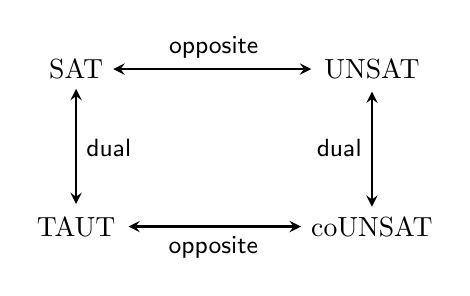
\begin{tikzpicture}[<->,>=stealth,shorten >=1pt,auto,node distance=2cm, thick,main node/.style={scale=0.9,circle,draw,font=\sffamily\normalsize}]

            \node[] (1) []{$\mathrm{SAT}$};
            \node[] (2) [right of = 1, xshift=50]{$\mathrm{UNSAT}$};
            \node[] (3) [below of = 1]{$\mathrm{TAUT}$};
            \node[] (4) [right of = 3, xshift=50]{$\mathrm{coUNSAT}$};

            \path[every node/.style={font=\sffamily\small}]
                (1) edge node{opposite} (2)
                (1) edge node{dual} (3)
                (4) edge node{dual} (2)
                (4) edge node{opposite} (3)
            ;
        \end{tikzpicture}

        \caption{Summary of the relations between types of satisfiability problems.}
    \end{figure}

    Now that we understand how disqualification and duality are two equivalent concepts for $\mathsf{NP}$ and $\mathsf{coNP}$, let's try to extend this concept to the class $\mathsf{P}$. By definition, we have that $\mathsf{coP} = \{L \subseteq \{0,1\}^* \mid \overline{L} \in \mathsf{P}\}$. However, we can easily see that these two classes are actually the same: if a language $L$ is decided by $M$ in polynomial time, then $\lnot M$ clearly decides $\overline{L}$ in polynomial time. Hence, we get that $\mathsf{P} = \mathsf{coP}$. This property is usually called \textbf{closure under complement}.

    We notice that the same argument cannot be used to show that $\mathsf{NP} = \mathsf{coNP}$: the opposite of a verifier is a disqualifier from the complementary language. Similarly, the opposite of a $\mathsf{NDTM}$ is not a valid $\mathsf{NDTM}$ for the complementary language: the original machine could have an accepting and a rejecting branch, hence the opposite machine would also have a rejecting and an accepting branch, but the latter may accept even strings that aren't in the complement of the original language.

    This property is an intrinsic difference between determinism and non-determinism. In fact, the opposite-machine-argument can be used to show that $\mathsf{EXP} = \mathsf{coEXP}$, but it doesn't work for the question $\mathsf{NEXP} \stackrel{?}{=}\mathsf{coNEXP}$.

    Since $\mathsf{P} \subseteq \mathsf{NP}$, through the first definition of $\mathsf{coNP}$ we easily get that $\mathsf{coP} \subseteq \mathsf{coNP}$. However, since the former is closed under complement, we conclude that $\mathsf{P} \subseteq \mathsf{coNP}$. This result can also be obtained through the second definition: for any pair $x,w$, we can ignore the witness and solve the problem on $x$ in polynomial time. Moreover, the second definition also allows us to show that $\mathsf{coNP} \subseteq \mathsf{EXP}$: we can just enumerate all the possible witnesses and check them deterministically in exponential time.

    Moreover, this closure under complement property of the class $\mathsf{P}$ can be used show that if $\mathsf{P} = \mathsf{NP}$ then trivially $\mathsf{NP} = \mathsf{P} = \mathsf{coP} = \mathsf{coNP}$. By contrapositive, we get the following theorem.

    \begin{framedthm}{}
        If $\mathsf{coNP} \neq \mathsf{NP}$ then $\mathsf{P} \neq \mathsf{NP}$
    \end{framedthm}

    This result gives us our first way to potentially show that $\mathsf{P} \neq \mathsf{NP}$. Nowadays, researchers believe that $\mathsf{coNP} \neq \mathsf{NP}$ is true, but none has yet proven it. The hardness of this question follows from the fact that a language can be \textsf{NP}-Complete if and only if its complement is \textsf{coNP}-Complete. Here, the concept of \textsf{coNP}-Completeness follows the same definition of \textsf{NP}-Completeness, where $\mathsf{NP}$ is replaced by $\mathsf{coNP}$. 

    \begin{framedthm}{}
        $L$ is \textsf{NP}-Complete if and only if $\overline{L}$ is \textsf{coNP}-Complete.
    \end{framedthm}
    
    \begin{proof}
        Suppose that $B$ is \textsf{NP}-Complete. Since $B \in \NPclass$, we trivially get that $\overline{B} \in \mathrm{coNP}$. Moreover, since $B$ is also \textsf{NP}-Hard, we know that for each problem $A \in \NPclass$ there is a function $f$ such that $x \in A$ if and only if $f(x) \in B$. We notice that this very same functions is also a reduction from the complement of $A$ to the complement of $B$ since $x \notin A$ if and only if $f(x) \notin B$. Hence, for each problem $\overline{A} \in \mathsf{coNP}$, we have that $\overline{A} \leq_m \overline{B}$
    \end{proof}

    If we are able to show that an $\mathsf{NP}$-Complete problem (or a $\mathsf{coNP}$-Complete one) also lies inside $\mathsf{coNP}$ (or $\mathsf{NP}$), then $\mathsf{NP} = \mathsf{coNP}$. However, this is equal to proving that $\mathsf{NP}$-Completeness and $\mathsf{coNP}$-Completeness are the same thing, which is indeed an extremely hard question.

    Furthermore, the previous theorem automatically implies that $\overline{\mathrm{SAT}}$ is \textsf{coNP}-Complete. Despise opposite and complementary problems being two very distinct things, we can actually always reduce the complementary problem to the opposite problem and vice versa. For instance, consider the following machine:

    $M$ = "Given the input string $x$:
    \begin{enumerate}
        \item Check if $x = \abk{\phi}$ for some formula $\phi$.
        \item If true, return $x$. Otherwise, return $\abk{y \land \lnot y}$"
    \end{enumerate}

    The trick here is to map every string that isn't a valid encoding of an unsatisfiable CNF formula to a pre-fixed unsatisfiable formula, i.e. the formula $y \land \lnot y$, while every string that is a valid gets mapped to itself. This reduction implies that $\overline{\mathrm{SAT}} \leq_P \mathrm{UNSAT}$, meaning that $\mathrm{UNSAT}$ is \textsf{coNP}-Hard. Moreover, this problem is also clearly in \textsf{coNP}: the disqualifying witness is an assignment that satisfies the formula. Hence, we get that $\mathrm{UNSAT}$ is \textsf{coNP}-Complete. The same trick can be used in reverse: we map every formula that is in $\mathsf{UNSAT}$ to itself, while gibberish strings are mapped to a satisfying formula, concluding that $\mathrm{UNSAT} \leq_P \overline{\mathrm{SAT}}$.

    Moreover, when a problem is the dual of the opposite (or the opposite of the dual) of a problem, we can often reduce the former to the latter and vice versa. For instance, the problem $\mathrm{UNSAT}$ can easily be reduced to the problem $\mathrm{TAUT}$: a CNF formula $\phi$ is unsatisfiable if and only if the DNF formula $\lnot \phi$ is a tautology, hence $\mathrm{UNSAT} \leq_P \mathrm{TAUT}$. This implies that $\mathrm{TAUT}$ is also \textsf{coNP}-Complete.

    \begin{figure}[H]
        \centering

        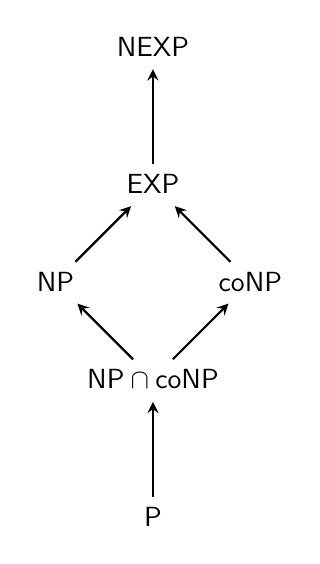
\begin{tikzpicture}[->,>=stealth,shorten >=1pt,auto,node distance=1.75cm,thick,main node/.style={scale=0.8,circle,draw,font=\sffamily\normalsize}]
            \node[] (1) []{$\mathsf{P}$};

            \node[] (2) [above of=1] {$\mathsf{NP} \cap \mathsf{coNP}$};
            \node[] (3) [above left of=2] {$\mathsf{NP}$};
            \node[] (4) [above right of=2] {$\mathsf{coNP} $};

            \node[] (5) [above right of=3] {$\mathsf{EXP}$};
            \node[] (6) [above of=5] {$\mathsf{NEXP}$};

            \path[every node/.style={font=\sffamily\small}]
                (1) edge (2)
                (2) edge (3)
                (2) edge (4)
                (3) edge (5)
                (4) edge (5)
                (5) edge (6)
                ;
        \end{tikzpicture}

        \caption{Summary of the class inclusions discussed in this chapter}
    \end{figure}
    

    \chapter{Diagonalization and Hierarchies}

    \section{Time Hierarchy theorems}
    \label{hier_thm}

    In \Cref{uncomputable} we discussed how the \textit{diagonal argument} can be used to prove that uncomputable functions exist. This argument is quite useful in order to prove many other theorems in the field of computational complexity. In particular, we're interested in showing the \textbf{hierarchy theorems}. These theorems highlight a fundamental property of computation: as we permit more resources, the computational power of the model strictly increases. This result may seem trivial, but it actually provides insights into the structural distinctions between different classes, underscoring the trade-offs between resource constraints and computational capability.
    
    In this chapter we'll discuss the \textbf{Time Hierarchy Theorem} proved by \textcite{det_time_hierarchy}, which shows that allowing Turing machines more computation time strictly increases the set of decidable languages. Other hierarchy theorems will be discussed in following chapters.

    \begin{framedthm}[label=dtime_hier]{Determinisitc Time Hierarchy Theorem}
        For all functions $f, g : \N \to \N$ with $g$ time-constructible and $f(n) = o(g(n))$
        \[\mathrm{DTIME}(f(n)) \subsetneq \mathrm{DTIME}(g(n)\log g(n))\]
    \end{framedthm}

    \begin{proof}
        It trivially holds that $\mathrm{DTIME}(f(n)) \subseteq \mathrm{DTIME}(g(n)) \subseteq \mathrm{DTIME}(g(n) \log g(n))$. We will show that the inclusion between $f(n)$ and $g(n) \log g(n)$ is actually strict.

        Consider the following \TM $M$ defined as:

        $M$ = "Given the input string $x$:

        \begin{enumerate}[label={\arabic*.}]
            \item Compute $\abs{x} = n$
            \item Compute $g(n)$ in a time-constructible way
            \item Store the value $\ceil{g(n)}$ in a counter. If such counter ever reaches the value 0 during the following instructions, $M$ immediately \textit{rejects}.
            \item Check if $x = \alpha10^*$, where $M_\alpha$ is a \TM. If the interpretation fails, $M$ \textit{rejects}.
            \item Simulate $M_\alpha$ with input $x$. After each step of the simulation, decrement the counter by one.
            \item If $M_\alpha$ accepts, $M$ \textit{rejects}. Otherwise, $M$ \textit{accepts}"
        \end{enumerate}

        We notice that each step of the simulation run by $M$ has to decrement the counter, which has size $\log \ceil{g(n)}$, which requires $d \cdot \log g(n)$ steps, for some $d \in \R^+$, in each simulation step. We also notice that even if the simulated machine would go into infinite loops, the simulation done by $M$ will still halt when the counter reaches zero, meaning that $M$ always halts after at most $d \cdot g(n) \log g(n)$ steps (the logarithmic factor is due to the counter). Hence, we know that the language $L(M)$ can be decided in time $O(g(n) \log g(n))$.
        
        Through the diagonal argument, we know that there is an encoding $\beta \in \{0,1\}^*$ such that $L(M)$ is also decided by a \TM $M_\beta$. By way of contradiction, suppose that $M_\beta$ runs in time $f(n)$. By definition of little-oh notation, we have that:
        \[\forall c \in \R_{>0} \; \exists n_0 \in \N_{>0} \mid \forall n \geq n_0 \;\; f(n) < c \cdot g(n)\]

        Hence, given that $\frac{1}{d} \in \R^+$, we know that $\exists n_0 \in \N_{> 0}$ such that $\forall n \geq n_0$ it holds that $f(n) < \frac{1}{d} \cdot g(n)$, and thus that $d \cdot f(n) < g(n)$.
        
        Consider the input string $x = \beta 10^{n_0}$. Since $\abs{x} \geq n_0$, the simulation of $M_{\beta}$ done by $M$ will run in $f(n) < d \cdot f(n) < g(n)$ steps, thus the counter will never reach the value zero. This means that $M(x)$ will simulate all the computation of $M_\beta(x)$ and return the opposite result, hence we get that $x \in L(M)$ if and only if $x \notin L(M_\beta) = L(M)$, which is a contradiction. This concludes that $M_\beta$ cannot run in time $f(n)$, hence $\mathrm{DTIME}(f(n)) \subsetneq \mathrm{DTIME}(g(n) \log g(n))$.
    \end{proof}

    This hierarchy theorem can be used to give another proof of the fact that $\mathsf{P} \subsetneq \mathsf{EXP}$: for all $k \in \N$ we have that $n^k = o\rbk{\frac{2^n}{\log 2^n}}$, hence $\mathrm{DTIME}(n^k) \subsetneq \mathrm{DTIME}(2^n) \subseteq \mathrm{DTIME}(2^{n^h})$ for all $h > 1$. Since each $\mathrm{DTIME}(n^k)$ is strictly contained inside each $\mathrm{DTIME}(2^{n^h})$, this concludes that each $\mathrm{DTIME}(n^k)$ is strictly contained in $\mathsf{EXP}$, thus $\mathsf{P}$ is also strictly contained. For Non-deterministic Turing machines, \textcite{nondet_time_hierarchy} defined an even stronger hierarchy theorem, where the logarithmic factor is not needed. The idea is similar to the previous proof (with some little tweaking), so we will omit it.

    \begin{framedthm}{Non-deterministic Time Hierarchy Theorem}
        For all functions $f, g : \N \to \N$ with $g$ time-constructible and $f(n+1) = o(g(n))$
        \[\mathrm{NTIME}(f(n)) \subsetneq \mathrm{NTIME}(g(n))\]
    \end{framedthm}

    \begin{proof}
        Omitted.
    \end{proof}
    
    \newpage

    \section{Ladner's theorem}

    One of the striking aspects of \textsf{NP}-Completeness is that a surprisingly large number of \textsf{NP} problems turned out to be be \textsf{NP}-Complete. This phenomenon suggests a bold conjecture: every problem in \textsf{NP} is either in \textsf{P} or \textsf{NP}-Complete. In other words, this conjecture states that there is no \textsf{NP}-Intermediate language, i.e. a language in \textsf{NP} that is not in \textsf{P} and not \textsf{NP}-Complete.

    \begin{frameddefn}{\textsf{NP}-Intermediateness}
        A language $L \in \mathsf{NP}-\mathsf{P}$ is said to be \textbf{\textsf{NP}-Intermediate} if it also isn't \textsf{NP}-Complete.
    \end{frameddefn}
    
    If $\mathsf{P} = \mathsf{NP}$, this conjecture is trivially true since every problem in $\mathsf{P}$ is Karp reducible to each other. However, we believe that $\mathsf{P} \neq \mathsf{NP}$. In this case, the conjecture turns out to be false. \textcite{ladner} was able to prove that, under this assumption, there is an $\mathsf{NP}$-Intermediate language.
    
    \begin{framedthm}[label=ladner]{Ladner's theorem}
        If $\mathsf{P} \neq \mathsf{NP}$ then there is an $\mathsf{NP}$-Intermediate language.
    \end{framedthm}

    \begin{proof}
        For every function $f : \N \to \N$, we define $\mathrm{SAT}_f$ as the language of all the satisfiable formulas of length $n$ that are padded with $1^{n^{f(n)}}$.
        \[\mathrm{SAT}_f = \cbk{\abk{\phi01^{n^{f(n)}}} \mid \phi \in \mathrm{SAT}, \abs{\phi} = n}\]

        Consider now the function $H : \N \to \N$ such that $H(n)$ is the smallest number $i < \log \log n$ such that for every $x \in \{0, 1\}^*$ with $\abs{x} \leq \log n$, the machine $M_i$ (where $i$'s binary expansion acts as the encoding) computes $\mathrm{SAT}_H(x)$ within $i\abs{x}^i$ steps. If there is no such number $i$ then $H(n) = \log \log n$.
        
        We notice that the function $H$ is well defined: $H(n)$ determines membership in $\mathrm{SAT}_H$ of strings whose length is greater than $n$ and the definition of $H(n)$ only relies upon checking the status of strings of length at most $\log n$. In fact, we can easily define a recursive algorithm that computes $H(n)$ in time $O(n^3)$.

        \textbf{Claim:} $\mathrm{SAT}_H \in \mathsf{P}$ if and only if $H(n) = O(1)$. Moreover, if $\mathrm{SAT}_H \notin \mathsf{P}$ then $H(n) \to +\infty$.

        \begin{proof}[Proof of the claim.]
            Suppose that $\mathrm{SAT}_H \in \mathsf{P}$ and let $M$ the \TM that computes $\mathrm{SAT}_H$ in polynomial time, say $kn^k$ steps for some $k \in \N$. By definition of $H$, there must be a number $i$ satisfying the constraints. Moreover, since $M$ can encoded by infinitely many strings, we can assume that $i$ is large enough to imply that $k < i$ and $M = M_i$. Then, for $2^{2^i} < n$ we have that $H(n) \leq i$, hence $H(n) = O(1)$.

            Suppose now that $H(n) \leq c$ for some constant $c \in \R$. Then, $H$'s image is finite, hence there must be an $i$ such that $H(n) = i$ for infinitely many $n$. By way of contradiction, suppose that $M_i$ doesn't compute $\mathrm{SAT}_H$ within $in^i$ steps. Then, there must be an input $x$ such that for every $2^{\abs{x}} < n$ it holds that $H(x) \neq i$, raising a contradiction. Thus, we get that 
            \[\exists c \in \N \mid H(n) \leq c \implies \mathrm{SAT}_H \in \mathsf{P}\] 

            The previous implication can be used to get two results:
            \begin{itemize}
                \item If $H(n) = O(1)$ then clearly there is a constant $c \in \N$ such that $H(n) \leq c$, concluding that $H(n) = O(1)$ implies that $\mathrm{SAT}_H \in \mathsf{P}$
                \item The contrapositive implication states that if $\mathrm{SAT}_H \notin \mathsf{P}$ then $H(n) \to +\infty$.
            \end{itemize}
        \end{proof}

        The previous claim holds even without the assumption that $\mathsf{P} \neq \mathsf{NP}$. However, if we assume the latter, then the language $\mathrm{SAT}_H$ must be \textsf{NP}-Intermediate.

        Suppose that $\mathrm{SAT}_H \in \mathsf{P}$. Then, by the previous claim, we know that $\exists c \in \N$ such that $H(n) \leq c$. Hence, we can build a machine $M$ that takes a formula $\phi$ as input, pads it with $01^{n^c}$ and runs the polynomial algorithm for $\mathrm{SAT}_H$ in order to solve $\mathrm{SAT}$ in polynomial time, which would conclude that $\mathrm{SAT} \in \mathsf{P}$ and thus that $\mathsf{P} = \mathsf{NP}$, contradicting the assumption. Hence, $\mathrm{SAT}_H \notin \mathsf{P}$.
        
        Suppose now that $\mathrm{SAT}_H$ is $\mathsf{NP}$-Complete. This implies that there is a Karp reduction from $\mathrm{SAT}$ to $\mathrm{SAT}_H$ that runs in time $O(n^i)$ for some $i \in \N$. This means that, for large enough input lengths, the reduction must map instances of length $n$ in $\mathrm{SAT}$ to instances of $\mathrm{SAT}_H$ with length smaller than $n^{H(n)}$, since otherwise the reduction wouldn't be computed in $O(n^i)$ steps. Thus, for large enough formulae, the reduction must map  $\phi$ to $\psi 01^{H(\abs{\psi})}$ instead of $\psi 01^{n^{H(\abs{\psi})}}$.

        However, we already showed that $\mathrm{SAT}_H \notin \mathsf{P}$, thus the claim implies that $H(n) \to +\infty$. This means that the reduction can be used to -- in some sense -- recursively reduce the size of the formula, giving us a polynomial time algorithm for $\mathrm{SAT}$, again contradicting the assumption. Hence, $\mathrm{SAT}_H$ cannot be $\mathsf{NP}$-Complete.
        
    \end{proof}

    Ladner's theorem is a significant result in computational complexity theory. However, the problem used by the theorem is clearly artificial and \curlyquotes{weird}. Currently, no \curlyquotes{natural} problems are known to be $\mathsf{NP}$-Intermediate under the assumption that $\mathsf{P} \neq \mathsf{NP}$. Finding such problem would provide valuable insight on what characteristics make a problem computable in polynomial time or $\mathsf{NP}$-Complete.
    
    \label{g_iso}
    A good candidate for being a natural $\mathsf{NP}$-Intermediate is the \textit{graph isomorphism problem}, which asks to determine if two graphs are isomorphic to each other. This problem is known to be solvable in \textbf{quasi-polynomial time}, that is in $O(2^{\log^c n})$ or equivalently $O(n^{\log^{c-1} n})$, even without the assumption that $\mathsf{P} \neq \mathsf{NP}$.
    
    \section{Oracles and the limits of diagonalization}

    Quantifying the limits of diagonalization is not easy. For concreteness, let us say that a \textit{diagonal argument} is any technique that relies solely on the existence of an effective representation of Turing machines by strings and the ability of an Universal \TM to simulate any another without much overhead in running time or space. Any argument based only in these facts is treating machines as \textbf{black boxes}: the machine's internal workings do not matter. This implies that any diagonal argument is also valid for \textbf{oracle Turing machines}.
    
    \begin{frameddefn}{Oracle Turing machine}
        An \textbf{oracle} is a black-box device that can magically solve in $O(1)$ the decision problem for some language $O \subseteq \{0, 1\}^*$. An \textbf{oracle Turing machine} $M^O$ can query an oracle for $O$ through a \textit{special oracle tape} on which it can write a string $q \in \{0, 1\}^*$, go into a \textit{special oracle state} to activate the oracle. After the query, the oracle tape will contain $0$ if $q \notin O$ and $1$ if $q \in O$.
    \end{frameddefn}

    Clearly. if $O$ is a difficult language then this oracle gives a huge amount of power to the \TM $M^O$. For every language $O \subseteq \{0, 1\}^*$, we denote with $\mathsf{P}^O$ the set containing every language that can be decided by a polynomial-time deterministic \TM with access to an oracle for $O$. Likewise, $\mathsf{NP}^O$ is the set of every language that can be decided by a polynomial-time nondeterministic
    \TM with access to an oracle for $O$. It trivially holds that $\mathsf{P} \subseteq \mathsf{P}^O$ and $\mathsf{NP} \subseteq \mathsf{NP}^O$. These notations can be extended in an intuitive way. For instance, we have that:
    \[\mathsf{P}^\mathsf{P} = \bigcup_{O \in \mathsf{P}} \mathrm{P}^O\]

    Oracles make reasoning about computation very easy. For instance, consider an oracle for a language $O \in \mathsf{P}$. Then, we have that $\mathsf{P}^O = \mathsf{P}$: each query to the oracle can be replaced by an algorithm that solves $O$ in polynomial time. This clearly concludes that $\mathsf{P}^\mathsf{P} = \mathsf{P}$. Likewise, it's easy to see that for any $\mathsf{NP}$-Complete language $L$ it holds that $\mathsf{P}^L = \mathsf{P}^\mathsf{NP}$.

    The key fact about oracle \textsf{TM}s is that regardless of what the oracle $O$ is , the set of all \textsf{TM}s with access to $O$ satisfy the two properties of any diagonal argument: just like a standard machine, we can represent each oracle machine $M^O$ as strings and simulate such \TM using a Universal \TM $U^O$ that itself also has access to an oracle for $O$. Thus any result about Turing machine that are based on diagonalization can also be extended for oracle machines. Such concept is called \textbf{relativization}. Many results in complexity theory are based on such concept.

    However, relativization actually \textit{limits} the power of diagonalization: we can define two languages $A$ and $B$ for which $\mathsf{P}^A = \mathsf{NP}^A$ and $\mathsf{P}^B \neq \mathsf{NP}^B$ \cite{relativization_p_np}. We wont dive into this proof as it requires the languages $A$ an $B$ are both convoluted -- think of what we did for \nameref{ladner}.

    \begin{framedthm}{The Baker-Gill-Solovay Theorem}
        There are two languages $A$ and $B$ for which $\mathsf{P}^A = \mathsf{NP}^A$ and $\mathsf{P}^B \neq \mathsf{NP}^B$. 
    \end{framedthm}

    \begin{proof}
        Omitted
    \end{proof}

    This theorem implies that any diagonalization or simulation proof that solves the question $\mathsf{P} \stackrel{?}{=} \mathsf{NP}$ must have some \textit{non-relativizable constraint} that impose that the proof would cannot be translated into a result for oracle machines. Even though many results in complexity relativize, there are some notable exceptions that will be discussed in future chapters.


    \section{The polynomial hierarchy}

    We have already explored several methods for "capturing" the core characteristics of families of computational problems by demonstrating their completeness within certain natural complexity classes. This section advances this exploration by examining another family of natural problems whose complexity cannot be fully represented by nondeterminism alone. To capture these problems, we define the \textbf{Polynomial Hierarchy} (\textsf{PH}), which generalizes the classes \textsf{P}, \textsf{NP} and \textsf{coNP}.
    
    To motivate the study of \textsf{PH}, we focus on some computational problems that seem to
    not be captured by \textsf{NP}-Completeness. First, recall that we proved how \textit{independent set problem} is \textsf{NP}-Complete.
    \[\mathrm{IND\text{-}SET}(x) = \soe{ll}{
        1 & \text{if $x = \abk{G,k}$ and $G$ is a graph with an ind. set $S$ of size $\abs{S} \geq k$} \\
        0 & \text{otherwise}
    }\]

    In order to certify that $\abk{G,k} \in \mathrm{IND\text{-}SET}$, any independent set of size $k$ can act as a polynomial sized witness. Now, consider the following variation of the independent set problem, i.e. the \textit{exact independent set problem}:
    \[\mathrm{EX\text{-}IND\text{-}SET}(x) = \soe{ll}{
        1 & \text{if $x = \abk{G,k}$ and $G$ is a graph whose largest ind. set is of size $k$} \\
        0 & \text{otherwise}
    }\]

    By definition, $\abk{G, k} \in \mathrm{EX\text{-}IND\text{-}SET}$ if and only if there is an independent set of size $k$ in $G$ and every other independent set has size
    at most $k$. In this case, the only possible certificate seems to be the set of all the independent sets of $G$, which requires exponential length in the worst case. This means that it probably holds that $\mathrm{EX\text{-}IND\text{-}SET} \notin \mathsf{NP}$.

    To better underline the difference between these two problems, let's rewrite their languages through \textit{quantifiers}:
    \[\mathrm{IND\text{-}SET} = \{\abk{G,k} \mid \exists S \text{ ind. set such that } \abs{S} \geq k\}\]
    \[\mathrm{EX\text{-}IND\text{-}SET} = \{\abk{G,k} \mid \exists S \text{ ind. set such that }\forall S' \text{ ind. set } \abs{S'} \leq \abs{S} = k\}\]

    The difference between the two problems seems to rely on the presence of an \textbf{additional universal quantifier} after the existence quantifier. This universal quantifier is what makes the witness too large. To bypass this issue, we can extend the concept of verification by \textit{splitting} the process of verification in two parts: one for the existential quantifier and one for the universal quantifier. We define the class $\Sigma_{2}^P$ as the set of languages for which there is a polynomial time \TM $M$ and a polynomial $q$ such that:
    \[L \in \Sigma_2^P \iff \forall x \in L \; \exists u \in \{0,1\}^{q(\abs{x})} \; \forall v \in \{0,1\}^{q(\abs{x})} \; M(x,u,v) = 1\]

    We observe that in this case the exponent $P$ is just a notation and thus \underline{not related to oracles}. This class is an extension of the class $\mathsf{NP}$: we can just ignore the universal quantifier. Hence, it holds that  $\mathsf{NP} \subseteq \Sigma_{2}^P$. We can easily show that $\mathrm{EX\text{-}IND\text{-}SET} \in \Sigma_2^P$: just use the existential verification for the maximum cardinality independent set and the universal verification for every other independent set.

    Now, consider the opposite problems $\mathrm{opIND\text{-}SET}$ and $\mathrm{opEX\text{-}IND\text{-}SET}$:
    \[\mathrm{opIND\text{-}SET} = \{\abk{G,k} \mid \forall S \text{ ind. set }\abs{S} \geq k\}\]
    \[\mathrm{opEX\text{-}IND\text{-}SET} = \{\abk{G,k} \mid \forall S \text{ ind. set }\exists S' \text{ind. set } \abs{S'} \leq \abs{S} = k\}\]

    We easily notice that $\mathrm{opIND\text{-}SET} \in \mathsf{coNP}$. However, for $\mathrm{opEX\text{-}IND\text{-}SET}$ we have the same issue as before: we need two quantifiers. To capture this language, we can extend the class \textsf{coNP} by defining the class $\Pi_{2}^P$ as the set of languages for which there is a polynomial time \TM $M$ and a polynomial $q$ such that:
    \[L \in \Pi_2^P \iff \forall x \in L \; \forall u \in \{0,1\}^{q(\abs{x})} \; \exists v \in \{0,1\}^{q(\abs{x})} \; M(x,u,v) = 1\]

    Interestingly, we notice that this class is still an extension of the class $\mathsf{NP}$: we can just ignore the universal quantifier. Hence, it holds that $\mathsf{NP} \subseteq \Pi_{2}^P$. In the same way, we also get that $\mathsf{coNP} \subseteq \Sigma_2^P$ and $\mathsf{coNP} \subseteq \Pi_2^P$. To create the polynomial hierarchy, we can generalize these two classes in order to allow for an alternating amount of existence and universal quantifiers (or viceversa).

    \begin{frameddefn}{The classes $\Sigma_i^P$ and $\Pi_i^P$}
        For $i \geq 0$, we define the class $\Sigma_i^P$ as the set of languages for which there is a polynomial time \TM $M$ and a polynomial $q$ such that $L \in \Sigma_i^P$ if and only if
        \[\forall x \in L \; Q_1 w_1  \; Q_2 w_2  \; \ldots \; Q_i w_i  \; M(x,w_1, \ldots, w_i) = 1\]

        where $Q_j$ is equal to $\exists$ if $j$ is odd and equal to $\forall$ if $j$ is even. Likewise, we define the class $\Pi_i^P$ as the set of languages for which there is a polynomial time \TM $M$ and a polynomial $q$ such that $L \in \Pi_i^P$ if and only if
        \[\forall x \in L \; Q_1 w_1  \; Q_2 w_2  \; \ldots \; Q_i w_i  \; M(x,w_1, \ldots, w_i) = 1\]
        where $Q_j$ is equal to $\forall$ if $j$ is odd and equal to $\exists$ if $j$ is even.
    \end{frameddefn}

    We notice that, by definition, we have that $\mathsf{P} = \Sigma_0^P = \Pi_0^P$, while $\mathsf{NP} = \Sigma_1^P$ and $\mathsf{coNP} = \Pi_1^P$. Generalizing the idea showed before, we notice that $\Sigma_i^P \subseteq \Pi_{i+1}^P$ and that $\Pi_i^P \subseteq \Sigma_{i+1}^P$. The \textbf{Polynomial Hierarchy} is formed of all the quantification levels:
    \[\mathsf{PH} = \bigcup_{i \geq 0} \textstyle \Sigma_i^P \displaystyle = \bigcup_{i \geq 0} \textstyle \Pi_i^P\]

    \begin{figure}[H]
        \centering

        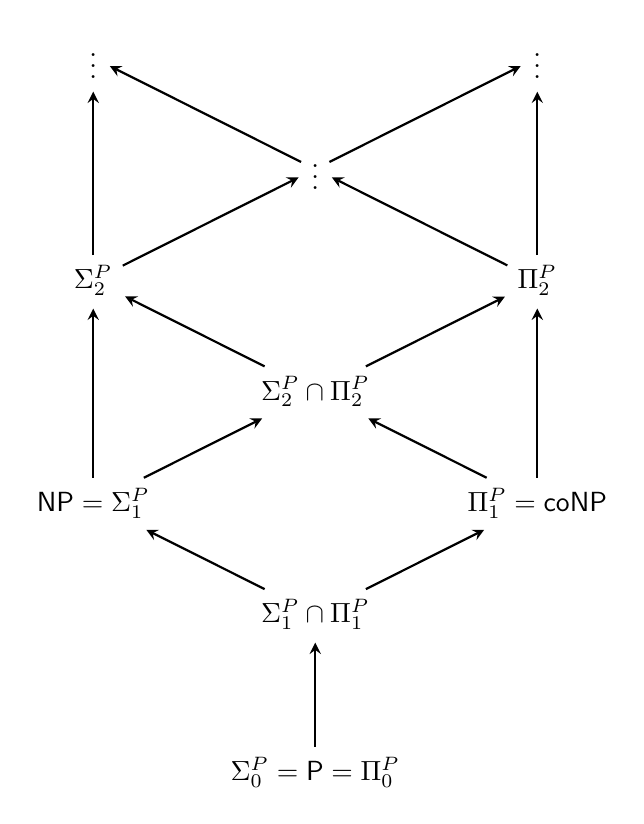
\begin{tikzpicture}[->,>=stealth,shorten >=1pt,auto,node distance=2cm,thick,main node/.style={scale=0.8,circle,draw,font=\sffamily\normalsize}]
            \node[] (1) []{$\Sigma_0^P = \mathsf{P} = \Pi_0^P$};

            \node[] (2) [above of=1] {$\Sigma_1^P \cap \Pi_1^P$};
            \node[] (3) [above left of=2, xshift=-40] {$\mathsf{NP} = \Sigma_1^P $};
            \node[] (4) [above right of=2, xshift=40] {$\Pi_1^P = \mathsf{coNP} $};

            \node[] (5) [above right of=3, xshift=40] {$\Sigma_2^P \cap \Pi_2^P$};
            \node[] (6) [above left of=5, xshift=-40] {$\Sigma_2^P$};
            \node[] (7) [above right of=5, xshift=40] {$\Pi_2^P$};

            \node[] (8) [above right of=6, xshift=40] {$\vdots$};
            \node[] (9) [above left of=8, xshift=-40] {$\vdots$};
            \node[] (10) [above right of=8, xshift=40] {$\vdots$};

            \path[every node/.style={font=\sffamily\small}]
                (1) edge (2)
                (2) edge (3)
                (2) edge (4)
                (3) edge (5)
                (3) edge (6)
                (4) edge (5)
                (4) edge (7)
                (5) edge (6)
                (5) edge (7)
                (6) edge (8)
                (6) edge (9)
                (7) edge (8)
                (7) edge (10)
                (8) edge (9)
                (8) edge (10)
                ;
        \end{tikzpicture}

        \caption{The polynomial hierarchy}
    \end{figure}

    Moreover, we also notice that $\Sigma_i^P = \mathsf{co}\Pi_i^P$ and thus $\Pi_i^P = \mathsf{co}\Sigma_i^P$. For instance, consider a language $L \in \Sigma_3^P$, hence we have that:
    \[x \in L \iff \exists w_1 \in \{0,1\}^{q(n)} \; \forall w_2 \in \{0,1\}^{q(n)} \; \exists w_3 \in \{0,1\}^{q(n)} \; M(x, w_1, w_2, w_3) = 1\]

    Hence, we have that:
    \[\begin{split}
        x \notin L &\iff \lnot(\exists w_1 \in \{0,1\}^{q(n)} \; \forall w_2 \in \{0,1\}^{q(n)} \; \exists w_3 \in \{0,1\}^{q(n)} \; M(x, w_1, w_2, w_3) = 1) \\
        &\iff \forall w_1 \in \{0,1\}^{q(n)} \; \lnot (\forall w_2 \in \{0,1\}^{q(n)} \; \exists w_3 \in \{0,1\}^{q(n)} \; M(x, w_1, w_2, w_3)  = 1) \\
        &\iff \forall w_1 \in \{0,1\}^{q(n)} \; \exists w_2 \in \{0,1\}^{q(n)} \; \lnot (\exists w_3 \in \{0,1\}^{q(n)} \; M(x, w_1, w_2, w_3)  = 1) \\
        &\iff \forall w_1 \in \{0,1\}^{q(n)} \; \exists w_2 \in \{0,1\}^{q(n)} \; \forall w_3 \in \{0,1\}^{q(n)} \; M(x, w_1, w_2, w_3)  = 0 \\
    \end{split}\]

    By defining a new machine $M'$ that returns the opposite of $M$, we conclude that:
    \[x \in \overline{L} \iff \forall w_1 \in \{0,1\}^{q(n)} \; \exists w_2 \in \{0,1\}^{q(n)} \; \forall w_3 \in \{0,1\}^{q(n)} \; M(x, w_1, w_2, w_3)  = 1\]
    
    concluding that $\overline{L}$ is in $\Pi_2^P$. Due to all the properties described above, the classes polynomial hierarchy are described as \curlyquotes{additional quantifying gadgets} applied to the class $P$.
    \[\Sigma_i^P = \underbrace{\exists \forall \exists \ldots}_{\text{$i$ times}} P \qquad\qquad \Pi_i^P = \underbrace{\forall \exists \forall \ldots}_{\text{$i$ times}} P\]
    
    The polynomial hierarchy can also be recursively described through \textbf{oracles}: for all $i \geq 1$, it holds that $\Sigma_i^P = \mathsf{NP}^{\Sigma_{i-1}^P}$ and that $\Pi_i^P = \mathsf{coNP}^{\Sigma_{i-1}^P}$. Following this idea, we can also define a new type of hierarchy level: for all $i \geq 0$, we define $\Delta_i^P = \mathsf{P}^{\Sigma_{i-1}^P}$. In particular, we have that $\Delta_i^P \subseteq \Sigma_i^P \cap \Pi_i^P$ and that $\mathsf{P} = \Delta_0^P = \Delta_1^P$.
    
    Interestingly, for each $i$-th level of the hierarchy we can define a \textbf{$\Sigma_i^P$-Complete} problem, i.e. the $\Sigma$-alternated quantified version of the satisfiability problem:
    \[\textstyle \Sigma_i^P\mathrm{SAT} \displaystyle = \{\abk{\phi} \mid Q_1 x_1 \; Q_2 x_2 \; \ldots \; Q_i x_i \; \phi(x_1, \ldots, x_i) = 1\}\]  
    where $Q_j$ is equal to $\exists$ if $j$ is odd and equal to $\forall$ if $j$ is even. Likewise, we can define a \textbf{$\Pi_i^P$-Complete} problem, i.e. the $\Pi$-alternated quantified version of the satisfiability problem:
    \[\textstyle \Pi_i^P\mathrm{SAT} \displaystyle = \{\abk{\phi} \mid Q_1 x_1 \; Q_2 x_2 \; \ldots \; Q_i x_i \; \phi(x_1, \ldots, x_i) = 1\}\]  
    where $Q_j$ is equal to $\forall$ if $j$ is odd and equal to $\exists$ if $j$ is even.

    We believe that $\mathsf{P} \neq \mathsf{NP}$ and $\mathsf{NP} \neq \mathsf{coNP}$ are through. An appealing generalization of these conjectures is that for every $i \geq 0$, it holds that  $\Sigma_i^P \subsetneq \Sigma_{i+1}^P$  and that $\Pi_i^P \subsetneq \Pi_{i+1}^P$. This conjecture is used often in complexity theory and is usually stated as \curlyquotes{the polynomial hierarchy does not collapse}, where the polynomial hierarchy is said to collapse if for some $j$ it holds that $\Sigma_j^P = \Sigma_{j+1}^P$. For instance, one can easily prove the following result by induction.

    \begin{framedthm}[label=ph_collapses]{Collapses of the Polynomial Hierarchy}
        For all $i \geq 1$, it holds that:
        \begin{enumerate}
            \item If $\Sigma_{i-1}^P = \Sigma_{i}^P$ then $\mathsf{PH} = \Sigma_{i-1}^P$
            \item If $\Pi_{i-1}^P = \Pi_{i}^P$ then $\mathsf{PH} = \Pi_{i-1}^P$
            \item If $\Sigma_i^P = \Pi_i^P$ then $\mathsf{PH} = \Sigma_i^P$
        \end{enumerate}
    \end{framedthm}

    \begin{proof}
        Omitted.
    \end{proof}

    As a corollary of this theorem, we get that if $\mathsf{P} = \mathsf{NP}$ then $\mathsf{P} = \mathsf{PH}$ and that if $\mathsf{NP} = \mathsf{coNP}$ then $\mathsf{NP} = \mathsf{PH}$. These two results should be enough evidence to believe that $\mathsf{P} \neq \mathsf{NP}$ and $\mathsf{NP} \neq \mathsf{coNP}$ are almost certainly true -- how could anyone believe such collapses?
    

    \chapter{Boolean circuits}

    \section{Boolean circuits and the class $\mathsf{P_{/poly}}$}

    Boolean circuits are defined as sets of logical AND, logical OR and logical NOT gates connected by cables. Boolean circuits have been proven to be Turing complete due to Turing machines and circuits being capable of simulating each other up to a polynomial factor. Again, no one should be dumbfounded by this result: any modern computer is just a large amount of Boolean gates wired together.

    \begin{frameddefn}{Boolean circuit}
    A \textbf{Boolean circuit} is a directed acyclic graph whose nodes, called gates, are  associated with either an input variable or a Boolean operator. Each input gate has in-degree 0 and unlimited out-degree. Each Boolean gate has an out-degree gate equal to 1 (except for the output gate which has out-degree 0) and in-degree equal to either 1 or 2. All the 1 in-degree gates compute the logical NOT and all 2 in-degree gates compute the logical AND or the logical OR of their given input variables or Boolean function.
    \end{frameddefn}
    
    Each gate $v$ is associated with the Boolean function $f_v$ computed by it. An assignment $x = x_1, \ldots, x_n$ defines the result of the computation for a gate. A function $f : \{0,1\}^n \to \{0,1\}$ is said to be computed by a circuit with output gate $u$ if for all inputs $x \in \{0,1\}^n$ it holds that $f(x) =  C(x)$, where $C(x)$ is the function computed by the output gate. 
    
    The complexity of Boolean circuits is measured in terms of their \textit{size} and \textit{depth}, i.e. the number of gates of the circuit and the length of the longest directed path from an input gate to the output gate. The \textbf{circuit complexity} of a function $f$ is defined as the size of the smallest Boolean circuit that computes it.

    \begin{figure}[H]
        \centering

        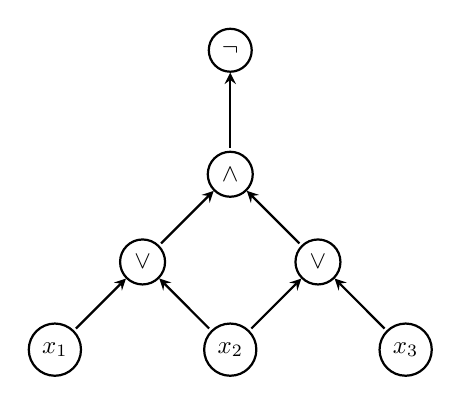
\begin{tikzpicture}[<-,>=stealth,shorten >=1pt,auto,node distance=1.75cm, thick,main node/.style={scale=0.9,circle,draw,font=\sffamily\normalsize}]

            \node[main node] (1) []{$\lnot$};
            \node[main node] (2) [below of = 1]{$\land$};
            \node[main node] (3) [below left of = 2]{$\lor$};
            \node[main node] (4) [below right of = 2]{$\lor$};
            \node[main node] (5) [below left of = 3]{$x_1$};
            \node[main node] (6) [below right of = 3]{$x_2$};
            \node[main node] (7) [below right of = 4]{$x_3$};

            \path[every node/.style={font=\sffamily\small}]
                (1) edge (2)
                (2) edge (3)
                (2) edge (4)
                (3) edge (5)
                (3) edge (6)
                (4) edge (6)
                (4) edge (7)
            ;
        \end{tikzpicture}

        \caption{A Boolean circuit of size 7 and depth 3 computing $\overline{(x_1 \lor x_2)(x_2 \lor x_3)}$.}
    \end{figure}

    Boolean circuits can also be defined in a different way. Instead of using logical NOT gates, we can assume that the the negations $\overline{x_1}, \ldots, \overline{x_n}$ are also input variables. Any standard circuit of size $S$ and depth $D$ can be easily transformed into this different type of circuit by repeatedly applying the De Morgan rule on all the logical NOT gates, producing a circuit of size at most $2S$ and depth at most $D$ due to the number of input gates being doubled and the logical NOT gates being removed. These circuits are usually called \textbf{De Morgan circuits}.

    \begin{figure}[H]
        \centering

        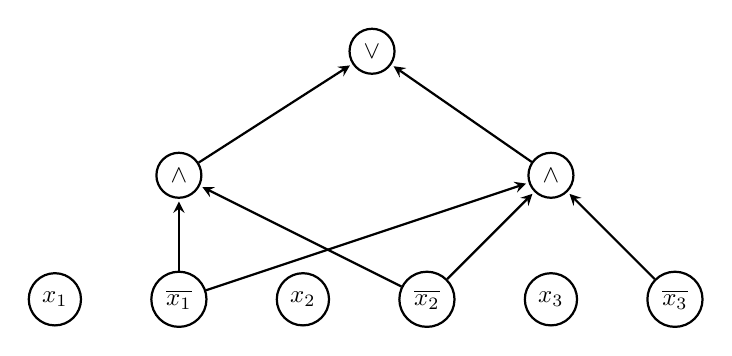
\begin{tikzpicture}[->,>=stealth,shorten >=1pt,auto,node distance=1.75cm, thick,main node/.style={scale=0.9,circle,draw,font=\sffamily\normalsize}]

            \node[main node] (1) []{$x_1$};
            \node[main node] (2) [right of = 1]{$\overline{x_1}$};
            \node[main node] (3) [right of = 2]{$x_2$};
            \node[main node] (4) [right of = 3]{$\overline{x_2}$};
            \node[main node] (5) [right of = 4]{$x_3$};
            \node[main node] (6) [right of = 5]{$\overline{x_3}$};
            \node[main node] (7) [above of = 2]{$\land$};
            \node[main node] (8) [above of = 5]{$\land$};
            \node[] (9) [right of = 7, xshift=20]{};
            \node[main node] (10) [above of = 9]{$\lor$};

            \path[every node/.style={font=\sffamily\small}]
                (2) edge (7)
                (2) edge (8)
                (4) edge (7)
                (4) edge (8)
                (6) edge (8)
                (7) edge (10)
                (8) edge (10)
            ;
        \end{tikzpicture}

        \caption{A De Morgan circuit of size 9 and depth 2 computing $\overline{(x_1 \lor x_2)(x_2 \lor x_3)}$.}
    \end{figure}

    \label{xor_circuit}

    An important thing to notice is that Boolean circuits do \textbf{not allow computations to be reused}. For example, consider the \textit{$n$ bit XOR function}:
    \[\mathrm{XOR}(x) = \bigoplus_{i = 1}^n x_i\]

    Intuitively, we can compute this function through recursion:
    \[(\lnot \mathrm{XOR}(x_1, \ldots, x_{\frac{n}{2}}) \lor \mathrm{XOR}(x_{\frac{n}{2}+1}, \ldots, x_{n})) \land (\mathrm{XOR}(x_1, \ldots, x_{\frac{n}{2}}) \lor \lnot \mathrm{XOR}(x_{\frac{n}{2}+1}, \ldots, x_{n}))\]

    \begin{figure}[H]
        \centering

        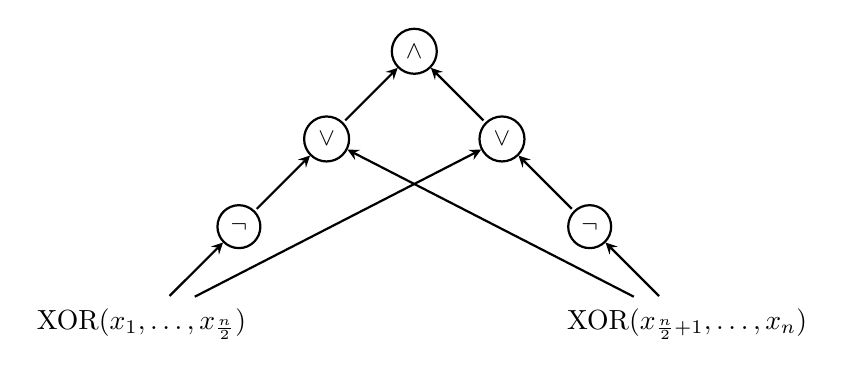
\begin{tikzpicture}[<-,>=stealth,shorten >=1pt,auto,node distance=1.75cm, thick,main node/.style={scale=0.9,circle,draw,font=\sffamily\normalsize}]

            \node[main node] (2) []{$\land$};
            \node[main node] (3) [below left of = 2]{$\lor$};
            \node[main node] (4) [below right of = 2]{$\lor$};
            \node[main node] (5) [below left of = 3]{$\lnot$};
            \node[main node] (6) [below right of = 4]{$\lnot$};
            \node[] (7) [below left of = 5]{$\mathrm{XOR}(x_1, \ldots, x_{\frac{n}{2}})$};
            \node[] (8) [below right of = 6]{$\mathrm{XOR}(x_{\frac{n}{2}+1}, \ldots, x_{n})$};

            \path[every node/.style={font=\sffamily\small}]
                (2) edge (3)
                (2) edge (4)
                (3) edge (5)
                (3) edge (8)
                (4) edge (6)
                (4) edge (7)
                (5) edge (7)
                (6) edge (8)
            ;
        \end{tikzpicture}

        \caption{Recursive computation of $\mathrm{XOR}(x)$}
    \end{figure}

    If we could model a circuit in this way, the size would be given by $S(n) = 5+2S\rbk{\frac{n}{2}}$, which is approximately $O(n)$. Without reusing computations, instead, we have to make two copies of each recursion.

    \begin{figure}[H]
        \centering

        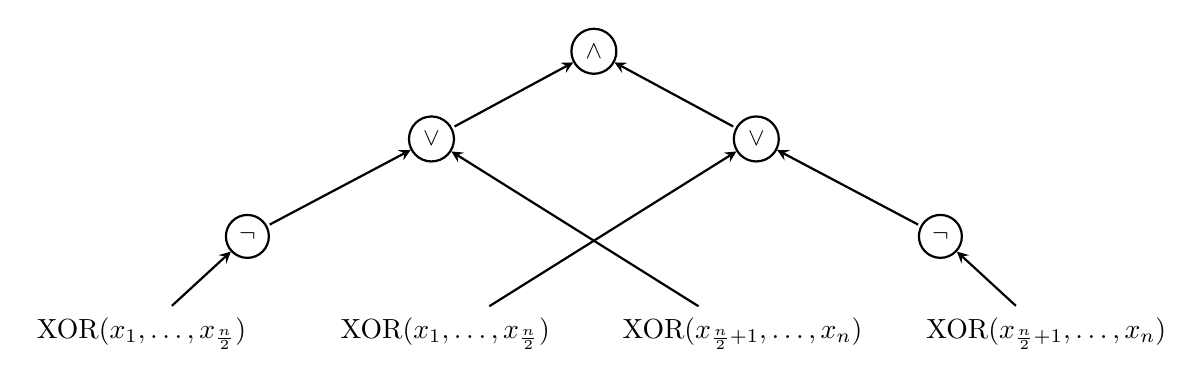
\begin{tikzpicture}[<-,>=stealth,shorten >=1pt,auto,node distance=1.75cm, thick,main node/.style={scale=0.9,circle,draw,font=\sffamily\normalsize}]

            \node[main node] (2) []{$\land$};
            \node[main node] (3) [below left of = 2, xshift = -30]{$\lor$};
            \node[main node] (4) [below right of = 2, xshift = 30]{$\lor$};
            \node[] (5) [below left of = 3]{};
            \node[] (6) [below right of = 4]{};
            \node[] (7) [below right of = 5, xshift=5]{$\mathrm{XOR}(x_1, \ldots, x_{\frac{n}{2}})$};
            \node[] (8) [below left of = 6, xshift=-5]{$\mathrm{XOR}(x_{\frac{n}{2}+1}, \ldots, x_{n})$};
            \node[] (9) [left of = 7, xshift=-60]{$\mathrm{XOR}(x_{1}, \ldots, x_{\frac{n}{2}})$};
            \node[] (10) [right of = 8, xshift=60]{$\mathrm{XOR}(x_{\frac{n}{2}+1}, \ldots, x_{n})$};

            \node[main node] (11) [left of = 5, xshift=15]{$\lnot$};
            \node[main node] (12) [right of = 6, xshift=-15]{$\lnot$};

            \path[every node/.style={font=\sffamily\small}]
                (2) edge (3)
                (2) edge (4)
                (3) edge (11)
                (3) edge (8)
                (4) edge (7)
                (4) edge (12)
                (11) edge (9)
                (12) edge (10)
            ;
        \end{tikzpicture}

        \caption{Recursive Boolean circuit that computes $\mathrm{XOR}(x)$}
    \end{figure}

    Hence, the size of the circuit is actually given by $S(n) = 5+4S\rbk{\frac{n}{2}}$, that is $O(n^2)$. Differently from Turing machines, circuits are capable of computing only functions with a fixed amount of input bits. To compute a variable input size, we need a \textit{family of circuits} $\{C_n\}_{n \in \N}$, where $C_n$ computes all the inputs of length $n$. 

    \begin{frameddefn}{Circuit family}
        A $T(n)$-size \textbf{circuit family} is a sequence $\{C_n\}_{n\in \N}$ of Boolean circuits, where $C_n$ has $n$ inputs, a single output and size at most $T(n)$. We say that a language $L$ is decidable by $(C_n)_{n\in \N}$ if $\forall x \in \{0,1\}^n$ it holds that $x \in L$ if and only if $C_n(x) = 1$.
    \end{frameddefn}

    Through circuit decidability, we can define an equivalent of the class \Pclass, i.e. the class $\mathsf{P_{/poly}}$. The notation \curlyquotes{/poly} comes from the equivalence between polynomial sized circuit families and Turing machines that take a polynomial amount of \curlyquotes{advice bits}, a topic that will be discussed in later sections. Circuit families are even capable of simulating non-advice-taking Oblivious Turing machines. This result will enable us to get many strong results, including the proof of \nameref{cook_levin} that we omitted before.

    \begin{frameddefn}{The class $\mathsf{P_{/poly}}$}
        We define the class of the languages decidable by a poly-sized circuit family:
        \[\mathsf{P_{/poly}} = \bigcup_{k \geq 0} \mathrm{SIZE}(n^k)\]
        where $\mathrm{SIZE}(f(n))$ is the set of all languages decided by a $f(n)$-sized circuit family
    \end{frameddefn}

    \begin{framedthm}[label={tm_circuit}]{Simulating \textsf{TM}s through circuit families}
        Let $L$ be a language decided by a \TM in time $T(n)$, where $T$ is time-constructable, and let $L_n = L \cap \{0,1\}^n$ for all $n \in \N$. There is a  circuit $C_n$ of size $c T(n)\log_2 T(n)$ such that $x \in L_n$ if and only if $C_n(x) = 1$
    \end{framedthm}

    \begin{proof}
        Let $M$ be a $k$-taped \TM that decides $L$ in time $T(n)$. We know that $M$ can be converted into an Oblivious \TM $M'$ that decides $L$ in time $T(n) \log_2 T(n)$. We'll use the obliviousness of this machine to build a single circuit $C_n$ that is capable of computing each string of length $n$.
        
        Let $T = T(n)\log_2 T(n)$. Let $z_1, \ldots, z_{T}$ be the sequence of \textit{snapshots} of the computation of $M'$. Each snapshot $z_i$ is a constant-sized string that encodes the machine's state and the $k$ symbols read by the $k$-heads. Since the machine is oblivious, this sequence of snapshots will be the same for each input of length $n$.
        
        Each snapshot $z_i$ can be computed by a constant-sized circuit that uses the input length $n$, the contents of the previous snapshot $z_{i-1}$ and the snapshots $z_{i_1}, \ldots, z_{i_k}$, where $z_{i_j}$ denotes the last step where the $j$-th head of $M'$ was in the same position as it is in the $i$-th step. In particular, the last sequence of snapshots acts as a \curlyquotes{control unit} that checks the correctness of the simulation by checking if the movements of the heads are legal. The AND of all the $T$ constant-sized circuits gives a circuit $C_n$ of size $O(T)$ such that $C_n(x) = M'(x)$ for all $x \in \{0,1\}^n$.
    \end{proof}

    \begin{figure}[H]
        \centering
        \includegraphics[scale=0.375]{images/tm_circuit.png}

        \textit{Encoding of an Oblivious \TM as a circuit for a specific input length}
    \end{figure}

    The previous result concludes that from each \TM that runs in time $T(n)$ we can build a circuit family $(C_n)_{n \in \N}$ that can decide the same language with size $cT (n) \log_2 T (n)$, giving us the following additional result.

    \begin{framedcor}{}
        $\mathsf{P} \subseteq \mathsf{P_{/poly}}$
    \end{framedcor}

    \section{Proof of the Cook-Levin theorem}

    We're finally ready to give a simple proof for \nameref{cook_levin}. Consider the following \textit{circuit satisfiability problem} as follows:
    \[\mathrm{CIRCUIT\text{-}SAT}(x) = \soe{ll}{
        1 & \text{if $x = \abk{C}$ and $C$ is a satisfiable circuit} \\
        0 & \text{otherwise}
    }\]
    
    A circuit is said to be satisfiable if there is at least one assignment of its variables such that $C(x) = 1$. Each circuit $C_n$ built in the conversion from a \TM to a circuit family can also be constructed in time $cT (n) \log_2 T (n)$. This allows us to prove that $\mathrm{CIRCUIT\text{-}SAT}$ is actually \NPclass-Complete.

    \begin{framedlem}{}
        $\mathrm{CIRCUIT\text{-}SAT}$ is \NPclass-Complete
    \end{framedlem}
    
    \begin{proof}
        
        $\mathrm{CIRCUIT\text{-}SAT}$ is clearly in \NPclass, since a satisfying assignment can act as a witness verifiable in polynomial time. We show that $\mathrm{CIRCUIT\text{-}SAT}$ is also \NPclass-Hard. Let $L$ be any language in $\NPclass$ and let $V$ be verifier of $L$ that runs in time at most $n^k$ for some $k \in \N$. We define a \TM $M$ as follows:
        
        $M$ = "Given the input string $x$:
        \begin{enumerate}
            \item Compute $n = \abs{x}$.
            \item Build the circuit $C_V : \{0,1\}^{n + n^k} \to \{0,1\}$ such that $C_V(x,\cdot) = V(x, \cdot)$ as described in \Cref{tm_circuit}
            \item Build the circuit $C_x : \{0,1\}^{n^k} \to \{0,1\}$ such that $C_x(\cdot) = C_V(x,\cdot )$
            \item Return $\abk{C_x}$"
        \end{enumerate}

        This machine computes a many-to-one reduction from $L$ to $\mathrm{CIRCUIT\text{-}SAT}$:
        \[x \in L \iff \exists w \in \{0,1\}^* \;\; V(x,w) = 1 \iff\]
        \[\exists w \in \{0,1\}^* \;\; C_x(w) = 1 \iff \abk{C_x} \in \mathrm{CIRCUIT\text{-}SAT}\]

        Since both $C_V$ and $C_x$ can be built in $c n^k \log_2(n^k)$, we conclude that this reduction is actually a Karp reduction.
    \end{proof}

    We now need to prove that $\mathrm{CIRCUIT\text{-}SAT} \leq_P \mathrm{CNF\text{-}SAT}$ holds. A trivial reduction would be to describe the entire circuit as a Boolean formula by mimicking it's gates. However, the final formula would not be in CNF, making the reduction invalid. To fix this, we convert the circuit to an \textit{equisatisfiable} CNF formula. We use \textit{Tseitin's transformation} \cite{tseitin}.

    \begin{framedlem}{Tseitin's transformation}
        $\mathrm{CIRCUIT\text{-}SAT} \leq_P \mathrm{CNF\text{-}SAT}$
    \end{framedlem}
    
    \begin{proof}
        Given a circuit $C$, let $S$ be its size. We encode each gate $g$ inside the circuit as a CNF subformula $\phi_g$:
        \begin{itemize}
            \item If $g$ is a logical NOT gate with the input gate $g_1$ then we define $\phi_g$ as:
            \[\phi_g = (g \to \overline{g_1})(\overline{g} \to g_1) = (\overline{g} \lor \overline{g_1})(g \lor g_1)\]
            This subformula evaluates as true if and only if $g = \lnot g_1$.

            \item If $g$ is a logical AND gate with input gates $g_1,g_2$, we define $\phi_g$ as:
            \[\phi_g = (g \to g_1 \land g_2)(\overline{g} \to \overline{g_1 \land g_2}) = (\overline{g} \lor g_1)(\overline{g} \lor g_2)(g \lor \overline{g_1} \lor \overline{g_2})\]
            This subformula evaluates as true if and only if $g =  g_1 \land g_2$.

            \item If $g$ is a logical OR gate with input gates $g_1,g_2$, we define $\phi_g$ as:
            \[\phi_g = (g \to g_1 \lor g_2)(\overline{g_1} \to \overline{g_1 \lor g_2}) = (\overline{g} \lor g_1 \lor g_2)(g \lor \overline{g_1})(g \lor \overline{g_2})\]
            This subformula evaluates as true if and only if $g =  g_1 \lor g_2$.
        \end{itemize}

        Let $\phi_C = \bigwedge_{i = 1}^S \phi_{g_i}$ be the formula that encodes every gate in $C$. This encoding perfectly describes the computation made by $C$. In order to force this computation, we consider the formula $\phi = g_S \land \phi_C$, in order to force that the output gate $g_S$ returns 1. In particular, we notice that without this last conjunction the formula $\phi_C$ is satisfiable even when the output gate doesn't return 1. Thus, we get that $C$ is satisfiable if and only if the $\phi$ is satisfiable. Moreover, since each subformula $\phi_g$ has at most 7 literals inside it, the final formula $\phi$ has at most $1+7S$ literals, implying that it can be constructed in polynomial time.
    \end{proof}

    With this lemma, we have finally completed the following Karp reduction chain:
    \[\mathrm{CIRCUIT\text{-}SAT} \leq_P \mathrm{CNF\text{-}SAT} \leq_P \mathrm{3\text{-}SAT} \leq_P \mathrm{SAT}\]
    Since $\mathrm{CIRCUIT\text{-}SAT}$ is \NPclass-Complete, through transitivity of Karp reductions we get that all these problems are \NPclass-Complete, finally concluding the proof of the Cook-Levin theorem!
    
    \newpage

    \section{Machines that take advice and non-uniformity}

    As briefly mentioned before, the name of the class $\mathsf{P_{/poly}}$ comes from it's alternative definition through Turing machines that take bits of advice. As per the $\mathsf{NP}$ case, this was the original definition, which quickly got replaced once the equivalence with circuits was proven.
    But what does \curlyquotes{bits of advice} mean? The idea here is that if our machine has some tips on how the solution is formed, the computation can become stronger.

    \begin{frameddefn}{Advice-taking \TM}
        Given a computable function $f$ and a function $a : \N \to \N$, we say that $f$ is decided by a \textbf{\TM $M$ that takes $a(n)$ bits of advice} if there is a sequence $(\alpha_n)_{n \in \N}$, with $\alpha_n \in \{0,1\}^{a(n)}$, such that  $\forall x \in \{0,1\}^n$ it holds that $f(x) = 1$ iff $M(x,\alpha_{n}) = 1$
    \end{frameddefn}

    We observe that this definition is \underline{different} from the concept of witness. In a verifier, we have to check that the witness $w$ is actually valid, while in an advice-taking \TM we assume that the bits are always correct. The other major difference is how the additional strings are pre-fixed: given two inputs of the same size $x, x' \in \{0,1\}^n$, they can have two different witnesses $w, w' \in \{0,1\}^*$, but they must use the same $n$ bits of advice $\alpha_n$.

    \begin{framedthm}{The class $\mathsf{P_{/poly}}$ (2nd Definition)}
        We define the class of the languages decidable by a polynomial time \TM that takes a polynomial amount of bits of advice:
        \[\mathsf{P_{/poly}} = \bigcup_{k,h \geq 0} \mathrm{DTIME}(n^k)_{/n^h}\]
        where $\mathrm{DTIME}(f(n))_{/a(n)}$ is the set of all languages decided by a \TM that runs in time $f(n)$ and takes $a(n)$ bits of advice 
    \end{framedthm}

    \begin{proof}
        First, we notice that the same construction given in \Cref{tm_circuit} can be used to also simulate an advice-taking \TM by just adding gates for the advice. Vice versa, given $L \in \mathsf{P_{/poly}}$ we know that there is a sequence of poly-sized circuits $(C_n)_{n \in \N}$ that decides $L$. Let $(\alpha_n)_{n \in \N}$ be the sequence such that $\alpha_n = \abk{C_n}$ and let $a(n) = \abs{\alpha_n}$. We can construct a machine $M$ that for each $x \in \{0,1\}^n$ takes the additional input $\alpha_n \in \{0,1\}^{a(n)}$ and simulates $C_n$, meaning that $M(x, \alpha_n) = C_n(x)$. Since the circuits have polynomial size, $a(n)$ defines a  polynomial amount of advice bits.
    \end{proof}
    
    Advice-taking machines can decide any unary language with a single bit of advice. A language $L$ is said to be \textbf{unary} if $L \subseteq 1^*$. In other words, every string of the language is in the form $1^n$ for some $n \in \N$. Given a language $L$, we define a machine $M$ that first checks if the input $x$ is of the form $1^n$ for some $n \in \N$ and then reads a single bit of advice $a_n$ such that $a_n = 1$ if and only if $x \in L$. This result can also be proved through circuits: for each $n \in \N$, if $1^n \in L$ then we consider the circuit made of $n$ AND gates, otherwise we consider the circuit that always outputs 0.

    \begin{framedprop}{}
        Any unary language $L \subseteq 1^*$ is in $\mathrm{DTIME}(n)_{/1}$ and $\mathrm{SIZE}(n)$
    \end{framedprop}

    We already proved that $\mathsf{P} \subseteq \mathsf{P_{/poly}}$. In fact, advice-taking Turing machines are clearly at least as strong as standard ones. However, we can easily prove that this type of machine is indeed way stronger than the standard model. For example, consider the \textit{unary halting problem}:
    \[\mathrm{UHALT}(x) = \soe{ll}{
        1 & \text{if $x = 1^n$ and $\abk{n} = \abk{M,y}$ for some pair $(M,y)$ s.t. $M(y)$ halts} \\
        0 & \text{otherwise}
    }\]

    $\mathrm{UHALT}$ is clearly uncomputable by a \TM since otherwise we would be able to solve the halting problem. However, since this a unary language, we know that it is inside $\mathsf{P_{/poly}}$. This result concludes that $\mathsf{P_{/poly}}$ is different from every single class that we previously encountered and in particular that the inclusion $\mathsf{P} \subseteq \mathsf{P_{/poly}}$ is strict.

    \begin{framedcor}{}
        $\mathsf{P} \subsetneq \mathsf{P_{/poly}}$
    \end{framedcor}

    Since circuits can simulate Turing machines and decide even uncomputable problems, this clearly concludes that circuits are actually stronger than machines. But where does this weird difference in power come from? The answer is simple: in the definition we require the circuit family to simply \curlyquotes{exist}, even if we have no idea of how the circuits are constructed. In a Turing machine, the computation is \textbf{uniform}, meaning that the instructions that define the computation for all input lengths follow a \curlyquotes{general structure}. In a circuit family, instead, each input length could be computed by a circuit completely different from the others, giving us a \textbf{non-uniform} computation. In order for a \TM to be capable of simulating a circuit family, we need this family to also be uniform, i.e. capable of being generated through an algorithm. If this holds, we can simulate it through a Turing machine: we compute the input length, construct the according circuit and simulate it. If the family isn't uniform, this process cannot work since we would need an infinite amount of \curlyquotes{blueprints} for all the circuits of the family.

    \begin{frameddefn}{Uniform circuit family}
        A circuit family $(C_n)_{n \in \N}$ is said to be \textbf{uniform} if there is a \TM $M$ such that $\forall n \in \N$ it holds that $M(1^n) = \abk{C_n}$
    \end{frameddefn}

    We notice that the circuit family obtained through the conversion process given by \Cref{tm_circuit} is actually uniform since this very process can indeed be computed by a \TM. When an uniform circuit family is also poly-sized, we say that it is $\mathsf{P}$-uniform. It's easy to see that the class of languages decidable by a $\mathsf{P}$-uniform circuit family is equivalent to the class $\mathsf{P}$, hence a language $L$ is in $\mathsf{P}$ if and only if it is decidable by a $\mathsf{P}$-uniform circuit family.

    \section{The Karp-Lipton theorem}

    We discussed how $\mathsf{P} \subseteq \mathsf{P_{/poly}}$ through circuits being capable of simulating a Turing machine computation. However, the same technique used in the proof of \cref{tm_circuit} cannot be used for verifiers since each input have a witness of different length, hence we cannot make the computation oblivious. Since $\mathsf{P} \subseteq \mathsf{P_{/poly}}$, if we were able to show that $\mathsf{NP} \not\subseteq \mathsf{P_{/poly}}$ then we would automatically conclude that $\mathsf{P} \neq \mathsf{NP}$. The \textbf{Karp-Lipton theorem} \cite{karp_lipton} gives us some insight to believe that $\mathsf{NP} \not\subseteq \mathsf{P_{/poly}}$ should be true.
    
    \begin{framedthm}[label=karp_lipton]{The Karp-Lipton theorem}
        If $\mathsf{NP} \subseteq \mathsf{P_{/poly}}$ then $\mathsf{PH} = \Sigma_2^P$
    \end{framedthm}

    \begin{proof}
        We want to show that $\Pi_2^P\mathrm{SAT} \leq_P \Sigma_2^P\mathrm{SAT}$ in order to prove that $\Pi_2^P \subseteq \Sigma_2^P$ holds if $\mathsf{NP} \subseteq \mathsf{P_{/poly}}$. The theorem will immediately follow from \Cref{ph_collapses}.

        \textbf{Claim}: If $\mathsf{NP} \subseteq \mathsf{P_{/poly}}$ then $\Pi_2^P\mathrm{SAT} \leq_P \Sigma_2^P\mathrm{SAT}$

        \begin{proof}[Proof of the claim]
        
            We recall that $\Pi_2^P\mathrm{SAT}$ is $\Pi_2^P$-Complete and that it is defined as:
            \[\abk{\phi} \in \Pi_2^P\mathrm{SAT} \iff \forall u \in \{0,1\}^n \; \exists v \in \{0,1\}^n \; \phi(u,v) = 1\]

            Let $\phi_u(v) = \phi(u,v)$. If $\mathsf{NP} \subseteq \mathsf{P_{/poly}}$ then we know that $\mathrm{SAT} \in \mathsf{P_{/poly}}$. Hence, there is a poly-sized circuit family $\{C_m\}_{m \in \N}$ that solves $\mathrm{SAT}$, implying that:
            \[\exists v \in \{0,1\}^n \; \phi_u(v) = 1 \iff \abk{\phi_u} \in \mathrm{SAT} \iff C_n(\abk{\phi_u}) = 1 \]

            Now, consider the idea we discussed in \Cref{decision_all} on how if $\mathsf{NP} \subseteq \mathsf{P}$ then search problems can be computed through decision problems. Here, we have a similar situation: if $\mathsf{NP} \subseteq \mathsf{P_{/poly}}$ then we can use circuits to solve search problems. In particular, we're interested in solving the search problem that finds a string $v \in \{0,1\}^n$ for any given a formula $\phi$ and $u \in \{0,1\}^n$ such that $\phi_u(v) = 1$. We know that there is a new poly-sized circuit family $(C'_m)_{m \in \N}$ such that for every formula $\phi$ and $u \in \{0,1\}^n$ if there is a string $v \in \{0, 1\}^n$ for which $\phi_u(v) = 1$ then $C'_n (\abk{\phi_u}) = v$ (we didn't formally define circuits with multiple bit outputs, but their definition follows as a natural extension).
            
            Due to non-uniformity, we only know that this circuit family exists, but we do not know how it is made. The idea here is that the circuits of this family can be \curlyquotes{guessed} using an additional existence quantification. Let $q$ be the the polynomial that defines the size of $(C'_m)_{m \in \N}$. We notice that each circuit in this family can be encoded with $O(q(n)^2)$ bits. Hence, each circuit can be guessed:
            \[\exists C'_n \in \{0,1\}^{O(q(n)^2)} \; \forall u \in \{0,1\}^n \; \phi(u, C'_n(\abk{\phi_u})) = 1\]
            This implies that $\abk{\phi} \in \Pi_2^P\mathrm{SAT}$ if and only if $\abk{\phi} \in \Sigma_2^P\mathrm{SAT}$. 
        \end{proof}

        Since $\Pi_2^P \subseteq \Sigma_2^P$ holds, thanks to duality we also get that $\Sigma_2^P = \mathsf{co}\Pi_2^P \subseteq \mathsf{co}\Sigma_2^P = \Pi_2^P$, hence we conclude that $\Pi_2^P \subseteq \Sigma_2^P$. By \Cref{ph_collapses}, we get that $\mathsf{PH} = \Sigma_2^P$.

    \end{proof}

    \newpage

    \section{Lower and upper bounds for circuits}

    Existing lower bounds for circuits are usually proved through the so-called \textbf{gate elimination argument}. The proofs themselves consist of a rather involved case analysis and we will not present them here. Instead, we will show the idea behind this type of proof by proving weaker lower bounds.

    The gate-elimination argument does the following: given a circuit for the function
    in question, we first argue that some variable $x_1$ (or a set of variables $x_1, \ldots, x_k$) must fan out to several gates. If we replace this variable with a constant value, also called \textbf{1-bit restriction}, several gates will be eliminated. For instance, given a gate $x_1 \lor x_2$, if we set $x_1$ then the whole gate can be eliminated. By repeatedly applying this process, we can conclude the number of gates in the original circuit. For a Boolean function $f$, we denote with $f_{\mid x_i = b}$ the 1-bit restriction of $f$ where the $i$-th variable gets replaced with the constant $b$:
    \[f_{\mid x_i = b}(x_1, \ldots, x_{i-1}, x_{i+1}, \ldots, x_n) = f(x_1, \ldots, x_{i-1}, b, x_{i+1}, \ldots, x_n)\]

    Consider the Boolean function $\mathrm{XOR}(x) = \bigoplus_{i = 1}^n x_i$. We already showed in \Cref{xor_circuit} that this function can be computed by a circuit of size $O(n^2)$. We will now prove a lower bound on the number of AND and OR gates of a circuit that computes such function.

    \begin{framedprop}{Circuit lower bounds on parity functions}
        Any circuit that computes $\mathrm{XOR}$ or $\lnot \mathrm{XOR}$ on $n$ bits requires at least $3(n-1)$ AND gates and OR gates.
    \end{framedprop}

    \begin{proof}
        Let $\mathrm{XOR}_k$ denote the $\mathrm{XOR}$ function applied to the first $k$ bits.
        
        \textbf{Claim:} In any circuit $C$ that computes $\mathrm{XOR}_k$ or $\lnot \mathrm{XOR}_k$ over $k \geq 2$ bits, there is a 1-bit restriction that eliminates at least 3 gates of $C$.

        \begin{proof}[Proof of the claim]

            We prove the claim for the function $\mathrm{XOR}_k$. The same argument can be applied to $\lnot \mathrm{XOR}_k$. Let $g$ be the first AND or OR gate (starting from the bottom) of an optimal circuit that computes $\mathrm{XOR}_k$ on $k$ bits. Let $x_i, x_j$ be its two inputs.
            
            Suppose now that $x_i$ has out-degree 1. This would imply that $g$ is the only gate with $x_i$ acting as an input. Then, we could replace $x_j$ with a constant $b$ such that $g_{\mid x_j = b_1}$ is equal to a constant bit $d_1$ (e.g. if $g = x_i \land x_j$ we can replace $x_j$ with 0 in order to also replace $g$ with 0). This would imply that for any assignment where $x_j = b_1$ the output of the circuit is independent of the value of $x_i$, which cannot happen by definition of the $\mathrm{XOR}_k$ function itself. Hence, $x_i$ must have at least 2 outgoing edges.
            
            Let $h$ be another gate for which $x_i$ acts as an input. We notice that $h$ cannot be the output gate of the circuit: if it wes, we could replace $x_i$ with a constant $b_1$ such that $h_{\mid x_i = b_2}$ is equal to a constant bit $d_2$, making the $\mathrm{XOR}_k$ function dependent only on the value of $x_i$, which is impossible. Hence, $h$ must have a successor gate $p$.

            Moreover, since we chose $g$ as the first AND or OR gate of the circuit, we know that $g$'s inputs can only be variables. Hence, we get that $g \neq p$. To recap, we have that $g,h,p$ are three different gates, where $x_i$ is the input of $g$ and $h$ and $h$ is the input of $p$.

            We notice that for any value $b_3 \in \{0,1\}$ we get that both $g_{x_i = b_3}$ and $h_{x_i = b_3}$ can be replaced by two constants. However, one of the two values is such that $p_{\mid x_i = b_3}$ can also be replaced by a constant. Hence, we conclude that there is a 1-bit restriction such that $g,h,p$ can be replaced.
        \end{proof}
        
        We now proceed by induction. Clearly, when $n = 1$ we need no gates at all to compute both $\mathrm{XOR}_n$ and $\lnot \mathrm{XOR}_n$. making the result trivially true. Assume now that for $\mathrm{XOR}_{n-1}$ and $\lnot \mathrm{XOR}_{n-1}$ we need at least $3(n-2)$ gates. We notice that $\mathrm{XOR}_{n \mid x_n = b}$ is equal to either $\mathrm{XOR}_{n-1}$ or $\lnot \mathrm{XOR}_{n-1}$ for any value $b \in \{0,1\}$. Thus, since the restriction $\mathrm{XOR}_{n \mid x_n = b}$ eliminates 3 gates and $\mathrm{XOR}_{n-1}$ (or $\lnot \mathrm{XOR}_{n-1}$) requires at least $3(n-2)$ gates, we get that $\mathrm{XOR}_n$ must require at least $3(n-2) + 3 = 3(n-1)$ gates.
    \end{proof}

    We now focus on upper bounds. Consider a generic function $f : \{0,1\}^n \to \{0,1\}$. Consider an assignment $\alpha$ such that $f(\alpha) = 1$. We define the logical formula $\phi_\alpha$ as the conjunction of all the literals described by $\alpha$. For instance, given a function $f : \{0,1\}^3 \to \{0,1\}$, if $\alpha = (1,0,1)$ is such that $f(\alpha) = 1$ then we have that $\phi_\alpha = (x_1 \land \overline{x_2} \land x_3)$.

    Consider now the formula $\phi = \bigvee_{\alpha : f(\alpha) = 1} \phi_\alpha$. This formula is a DNF for which $\phi(\alpha) = 1 \iff f(\alpha) = 1$. Each clause $\phi_\alpha$ can be computed by a sequence of $n$ AND gates. Let $C_\alpha$ be such sub-circuit that computes $\phi_\alpha$. The circuit that computes $\phi$ (and $f$) is given by a sequence of $k$ OR gates, where $k$ is the number of assignments such that $f$ accepts. Since the function $f$ has $2^n$ assignments, in the worst case all of them will be accepting, concluding that $k \leq 2^n$. Hence, we get the size upper bound of $n2^n$.

    This upper bound is clearly too high, but it is still sufficient to conclude that we only need circuits of at most exponential size to compute any Boolean function on $n$ inputs. \textcite{shannon} was able to give a better upper bound of $O(2^n)$, proving that we actually need only subexponential circuits.

    \begin{framedthm}[label=circ_up]{Shannon's size upper bound}
        Any function $f : \{0,1\}^n \to \{0,1\}$ can be computed by a circuit of size $O \rbk{\frac{2^n}{n}}$.
    \end{framedthm}

    \begin{proof}
        First, we notice that for any Boolean funcion $f : \{0,1\}^n \to \{0,1\}$ can be decomposed as:
        \[f(x_1, \ldots, x_{n-1}, x_n) = (x_n \land f(x_1, \ldots, x_{n-1}, 1)) \lor (\overline{x_n} \land f(x_1, \ldots, x_{n-1}, 0))\]

        Let $S(n)$ be the size complexity of $f$. The decomposition process described above can be recursively applied, giving the following recursive equation:
        \[S(n) \leq \soe{ll}{
            2S(n-1) + 3 & \text{if } n > 1 \\
            1 & \text{if } n = 1 \\
        }\]

        where the 3 gates are given by the two ANDs and the single OR -- we can ignore the NOT gate if we assume to be working with a DeMorgan circuit, since they require the same size up to a constant factor. By developing the recursive equation we get that:
        \[S(n) \leq 2^k S(n-k) + 3 \sum_{i = 0}^{k-1} 2^i = 2^k S(n-k) + 3(2^{k}-1)\]

        When $k = n-1$ we reach the base case, obtaining that $S(n) \leq O(2^{n})$. This decomposition process already gives us an improved upper bound (from $O(n2^n)$ to $O(2^n)$). However, Shannon also noticed that this decomposition process wastes a lot of gates. Consider now the set $Y_m$ of all functions from $\{0,1\}^m$ to $\{0,1\}$. This set contains exactly $2^{2^{m}}$ functions. When we reach a small enough recursion level, we're computing the same small functions over and over. For instance, we're computing $2^{n-3}$ functions taken from $Y_3$, even thought there are only $2^{2^3}$ functions inside $Y_3$. Hence, it is much more efficient to pre-compute these functions without applying the decomposition process.

        Let $\mathrm{All}_m : \{0, 1\}^m \to \{0, 1\}^{2^{2^m}}$ be the function that computes all the functions in $Y_m$ at the same time -- in other words, $\mathrm{All}_m(x) = (f_1(x), f_2(x), \ldots , f_{2^{2^m}} (x))$. Let $A(m)$ be the size of a circuit computing $\mathrm{All}_m$. By applying the decomposition process on $\mathrm{All}_m$, we observe that we need only one recursive circuit to compute $\mathrm{All}_{m-1}$ since it already computes all the functions in $Y_{m-1}$. Thus, we get that:
        \[A(m) \leq \soe{ll}{
            A(m-1) + 3 \cdot 2^{2^m} & \text{if } n > 1 \\
            2^{2^1} & \text{if } n = 1 \\
        }\]      
        
        By solving this recurrence, we have that $A(m) \leq 3 \cdot 2^{2^{m}} + 6\cdot 2^{2^{m-1}}$. We recall that $S(n)$ is the upper bound on the size complexity of a single function in $Y_n$. If we apply the decomposition process on this single function up to the $(n-m)$-th recursion, we get that $S(n) \leq 2^{n-m} S(m) + 3(2^{n-m}-1)$. As we discussed above, we can substitute the $2^{n-m}$ sub-circuits of size $S(m)$ with a single circuit that computes $\mathrm{All}_m$, implying that:
        \[S(n) \leq 2^{n-m} S(m) + 3(2^{n-m}-1) \leq A(m) + 3(2^{n-m}-1) \leq 3 \rbk{2^{n-m} +2^{2^{m}}} + 6\cdot 2^{2^{m-1}}\]

        By setting $m = \log n - 1$, we get that:
        \[\begin{split}
            S(n) &\leq 3 \rbk{2^{n-\log n + 1} +2^{2^{\log n -1}}} + 6\cdot 2^{2^{\log n -2}}\\
            &\leq 3 \rbk{\frac{2^{n+1}}{n} + 2^{\frac{n}{2}}} + 6 \cdot 2^{\frac{n}{4}} \\
            &\leq O\rbk{\frac{2^{n}}{n}} + O\rbk{2^{\frac{n}{2}}} \\
            &\leq O\rbk{\frac{2^{n}}{n}}
        \end{split}\]

    \end{proof}

    In the same paper, \textcite{shannon} also proved that almost every Boolean function cannot be computed by a sub-exponential size circuit. Together with his upper bound proof, Shannon's results show that \textbf{almost every Boolean function} strictly requires exponential size. This tells us that some functions are hard even for non-uniform circuits, implying that we should be able to find one such function that also happens to lie in \textsf{NP}, separating the two classes and thus proving that $\mathsf{P} \neq \mathsf{NP}$. However, since the lower bound theorem is only a counting argument, the structure of these hard functions is unknown. Hence, no one was able use this fact to show that $\mathsf{NP} \neq \mathsf{P_{/poly}}$. At the moment, the best circuit size lower bound for an \textsf{NP} language is only $5n - o(n)$.

    \begin{framedthm}[label=hard_circ]{Shannon's size lower bound}
        For every $n > 1$, with probability at least $1-o(1)$, a random function $f : \{0, 1\}^n \to \{0, 1\}$ requires a circuit of size greater than $\frac{2^n}{10n}$.
    \end{framedthm}

    \begin{proof}
        We prove the theorem through a simple counting argument. Let $C$ be a circuit of size at most $S$. We notice that $C$ can be encoded with $9 S \log S$ bits by representing it as an adjacency list. Let $X_S$ be the set of all the circuits of size at most $S$. We get that $\abs{X_S} = 2^{9 S \log S}$. Consider now the set $Y_n$ of all functions from $\{0,1\}^n$ to $\{0,1\}$. This set contains exactly $2^{2^{n}}$ functions. If $S = \frac{2^n}{10n}$, we notice that:
        \[\frac{\abs{X_S}}{{\abs{Y_n}}} =  \frac{2^{9 \frac{2^n}{10n}\log \rbk{\frac{2^n}{10n}}}}{2^{2^n}} = \frac{1}{2^{2^n \rbk{1-\frac{9}{10n}\log \rbk{\frac{2^n}{10n}}}}} < \frac{1}{2^{\frac{2^n}{10}}} = o(1)\]
        Hence, the probability of a random function to be computable by a circuit of size at most $\frac{2^n}{10n}$ is $o(1)$.
    \end{proof}

    Interestingly, Shannon's lower and upper bounds are sufficient to define a hierarchy theorem even for the size of non-uniform circuits. This result can also be proven through the standard diagonalization method.

    \begin{framedthm}{Non-uniform Hierarchy Theorem}
        For all functions $f, g : \N \to \N$ with $n < 10f(n) < g(n) < \frac{2^n}{n}$, it holds that 
        \[\mathrm{SIZE}(f(n)) \subsetneq \mathrm{SIZE}(g(n))\]
    \end{framedthm}

    \begin{proof}
        From \Cref{hard_circ}, we know that for each $\ell > 1$ there is a Boolean function $h : \{0,1\}^\ell \to \{0,1\}$ such that $h$ has size greater than $\frac{2^\ell}{10\ell}$. Moreover, from \Cref{circ_up} we know that for such function $h$ it holds that $h \in \mathrm{SIZE}\rbk{\frac{2^{\ell}}{\ell}}$ gates. Choose a value of $\ell$ such that $f(n) = \frac{2^{\ell}}{10\ell}$, trivially concluding that $h \notin \mathrm{SIZE}(f(n))$ since $h$ requires more gates. However, since $10 f(n) < g(n)$, we also know that:
        \[h \in \mathrm{SIZE}\rbk{\frac{2^{\ell}}{\ell}} = \mathrm{SIZE}\rbk{10 f(n)} \subseteq \mathrm{SIZE}\rbk{g(n)}\]
    \end{proof}

    \chapter{Randomized computation}

    \section{Randomization and the class \textsf{BPP}}

    Up until now, we've used the deterministic Turing machine as our standard model of computation. However, this model doesn't capture one important aspect of reality: the ability to make random choices during computation. For instance, most programming languages offer a built-in pseudo-random number generator for this purpose. While scientists and philosophers continue to debate the existence of true randomness, it's clear that outcomes like coin tosses—or other physical measurements—appear sufficiently random and unpredictable for practical use. Therefore, it's reasonable to consider Turing machines capable of simulating coin tosses through a source of random bits.

    \begin{frameddefn}{Probabilistic Turing machine}
        A \textbf{probabilistic Turing machine (PTM)} is a \TM provided with two
        distinct transition functions $\delta_0, \delta_1$ . On each step, the computation made by the machine \curlyquotes{flips a coin} and choses to apply $\delta_0$ or $\delta_1$ both with probability $\frac{1}{2}$. The running time of an \textsf{PTM} is the maximum number of steps that the computation may take regardless of the random choices that it makes.
    \end{frameddefn}

    We notice that this definition is similar to the one we gave for Non-deterministic Turing machines. In fact, \textsf{PTM}s may be seen as a \curlyquotes{restriction} of \textsf{NDTM}s. In the latter, the machine explores all the $2^{T(n)}$ paths in the \textbf{binary computation tree} at the same time through non-determinism. In \textsf{PTM}s, instead, the machine explores only one such path, which is chosen \textbf{randomly} in each computation with probability $\frac{1}{2^{T(n)}}$. However, even though they look similar, \textsf{PTM}s and \textsf{NDTM}s are very different: like \textsf{DTM}s, and unlike \textsf{NDTM}s, probabilistic machines are intended to model realistic computational devices.

    Now that we have formally defined how Turing machines can \curlyquotes{toss coins} to compute, we have to formally defined what it means for a language to be computed by such machines. We say that a language is decided by a \textsf{PTM} if such machine accepts strings in the language and rejects other strings with a \textbf{good bounded-error}. In particular, we require that this bounded-error at least $\frac{2}{3}$, both for accepted and rejected strings. We can define a new class \textsf{BPP}, standing for \textbf{bounded-error probabilistic polynomial time}.

    \begin{frameddefn}{The class $\mathsf{BPP}$}
        We define $\mathsf{BPP}$ as the class of languages for which there is a polynomial time \textsf{PTM} $M$ such that:
        \[x \in L \iff \Pr[M(x) = L(x)] \geq \frac{2}{3}\] 
        where $L(x) = 1$ if $x \in L$ and $L(x) = 0$ if $x \notin L$. The machine $M$ is often referred to as a \textbf{Monte Carlo machine}.
    \end{frameddefn}

    \begin{figure}[H]
        \centering

        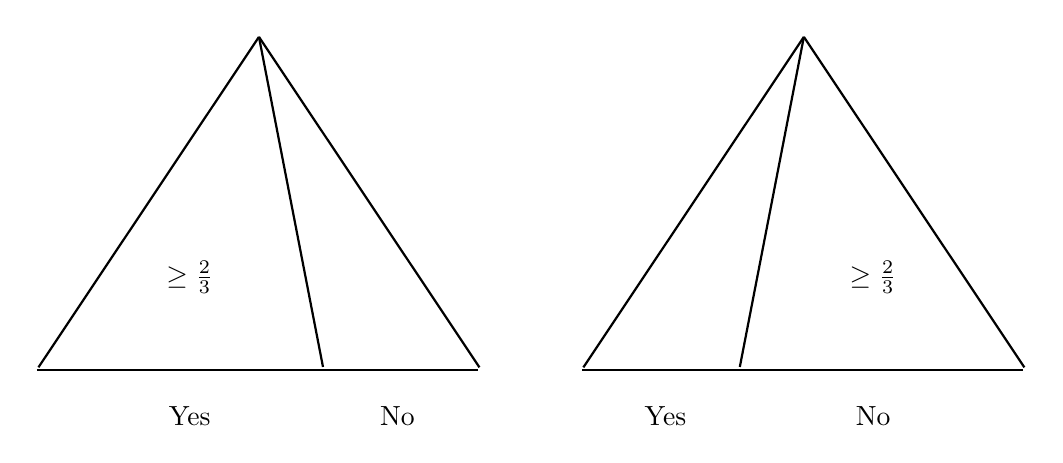
\begin{tikzpicture}[-,>=stealth,shorten >=1pt,auto,node distance=2cm, thick,main node/.style={scale=0.9,circle,draw,font=\sffamily\normalsize}]

            \node[] (1) []{};
            \node[] (2) [below left of = 1, xshift=-40, yshift=-80]{};
            \node[] (3) [below right of = 1, xshift=40, yshift=-80]{};
            \node[] (4) [left of = 3, xshift = 0]{};
            \node[] (5) [below of = 1, xshift = -25, yshift=-30]{$\geq \frac{2}{3}$};
            \node[] (6) [below of = 1, xshift = -25, yshift=-80]{Yes};
            \node[] (6) [below of = 1, xshift = 50, yshift=-80]{No};

            \node[] (1b) [right of = 1, xshift = 140]{};
            \node[] (2b) [below left of = 1b, xshift=-40, yshift=-80]{};
            \node[] (3b) [below right of = 1b, xshift=40, yshift=-80]{};
            \node[] (4b) [right of = 2b, xshift = 0]{};
            \node[] (5b) [below of = 1b, xshift = 25, yshift=-30]{$\geq \frac{2}{3}$};
            \node[] (6b) [below of = 1b, xshift = -50, yshift=-80]{Yes};
            \node[] (6b) [below of = 1b, xshift = 25, yshift=-80]{No};

            \path[every node/.style={font=\sffamily\small}]
                (1.center) edge (2.center)
                (1.center) edge (3.center)
                (2.center) edge (3.center)
                (1.center) edge (4.center)
                
                (1b.center) edge (2b.center)
                (1b.center) edge (3b.center)
                (2b.center) edge (3b.center)
                (1b.center) edge (4b.center)
            ;
        \end{tikzpicture}

        \caption{Distribution of branches for $\mathsf{BPP}$ when $x \in L$ (left) and when $x \notin L$ (right)}
    \end{figure}

    The idea behind this definition is that by running the machine $k$ times on the same input we will have the following probability table:
    \begin{center}
        \begin{tabular}{c|cc}
            & $L(x) = 1$ & $L(x) = 0$ \\
            \hline
            $M(x)= 1$ & $> 1- \frac{1}{2^{ck}}$ & $< \frac{1}{2^{ck}}$ \\
            $M(x)= 0$ & $< \frac{1}{2^{ck}}$ & $> 1- \frac{1}{2^{ck}}$
        \end{tabular}
    \end{center}
    For a sufficiently large $k$, we are pretty sure that the machine decides the language. 

    Since any deterministic \TM is a special case of a $\mathsf{PTM}$ where both transition functions are equal, it trivially holds that $\mathsf{P} \subseteq \mathsf{BPP}$. A central open question of complexity theory is whether or not $\mathsf{P} = \mathsf{BPP}$. Surprisingly, many complexity theorists actually believe that answer to the question $\mathsf{P} \stackrel{?}{=} \mathsf{BPP}$ is actually true. This derives from important results shown in the theory of \textit{de-randomization} and \textit{pseudo-randomization}. Moreover, it's also easy to see that $\mathsf{BPP} \subseteq \mathsf{EXP}$: we can build a deterministic \TM that simulates every possible sequence of coin tosses in exponential time.
    
    Moreover, we do not know if $\mathsf{BPP} \subseteq \mathsf{NP}$ or if $\mathsf{BPP} \subseteq \mathsf{coNP}$: any \textsf{PTM} computing a language in $\mathsf{BPP}$ may have an accepting and a rejecting branch both when $x \in L$ and $x \notin L$, thus it cannot be easily converted into an \textsf{NDTM}. 
    
    Surprisingly, probabilistic algorithms can sometimes be even more efficient that non-random ones. For instance, consider the search problem $\mathrm{MEDIAN}$ which asks to find the median of $n$ input numbers. This search problem is actually in $\mathsf{P}$ as it can be solved efficiently in $O(n \log n)$ by first sorting the numbers and then returning the middle element. However, we can solve this search problem in time $O(n)$ through randomization. In fact, we can solve an ever harder problem, i.e. finding the $k$-th smallest element in the set.

    $\mathtt{kSmallest}(k, a_1, \ldots, a_n)$:
    \begin{enumerate}
        \item Pick a random $i \in [n]$ and count the number $m$ of elements $a_j$ such that $a_j \leq a_i$
        \item If $m = k$, output $a_i$
        \item If $m > k$, output $\mathrm{kSmallest}(k, b_1, \ldots, b_m)$, where $b_1, \ldots, b_m$ are the $m$ elements counted before
        \item If $m < k$, output $\mathrm{kSmallest}(k, c_1, \ldots, c_{n-m})$, where $c_1, \ldots, c_{n-m}$ are the $n-m$ elements not counted before"
    \end{enumerate}

    In the worst case, the runtime is given by $T(n) = T \rbk{\frac{9}{10}n} + O(n)$, which is indeed $O(n)$. Moreover, this algorithm is actually guaranteed to always return the correct median value. There are indeed some non-randomized alternatives that can also run in $O(n)$, such as the \textit{median of medians} algorithm \cite{median_of_medians}, but they are based on way more complex techniques. The randomized algorithm that we provided is one of the most used in practice, showing that randomness can often be a very good tool.

    Without much surprise, the class \textsf{BPP} can also be defined through the concept of random verification: at least $\frac{2}{3}$ of the random paths will act as the witnesses through which a standard \TM can verify the membership.

    \begin{framedthm}{The class $\mathsf{BPP}$ (2nd Definition)}
        Given a language $L$, it holds that $L \in \mathsf{BPP}$ if and only if there is a polynomial time deterministic \textsf{TM} $M$ such that:
        \[x \in L \iff \Pr_{r \in_{R} \{0,1\}^*}[M(x,r) = L(x)] \geq \frac{2}{3}\] 

        \textit{Note}: the \curlyquotes{$\in_R$} symbol here denotes that $r$ is randomly chosen from $\{0,1\}^*$.
    \end{framedthm}

    The choice of the constant $\frac{2}{3}$ that we used up until now may seem pretty arbitrary. However, this choice is actually sufficient to form a robust definition. In fact, we now show that we can replace $\frac{2}{3}$ with any constant larger than $\frac{1}{2}$ or even with $\frac{1}{2} + \frac{1}{n^c}$ for any constant $c > 0$. We denote with $\mathsf{BPP}_c$ the class of languages $L$ for which there is a polynomial time \textsf{PTM} $M$ such that:
    \[\Pr[M(x) = L(x)] \geq \frac{1}{2} + \frac{1}{\abs{x}^c}\]
    for any $x \in \{0, 1\}^*$. Trivially, we have that $\mathsf{BPP} \subseteq \mathsf{BPP}_c$ for any $c > 0$. We show that $\mathsf{BPP}_c \subseteq \mathsf{BPP}$ also holds by proving an actually stronger result.

    \begin{framedthm}{Error reduction for $\mathsf{BPP}$}
        Given a language in $\mathsf{BPP}_c$, for every constant $d > 0$ there exists a polynomial time \textsf{PTM} $M$ such that for any $x \in \{0, 1\}^*$ it holds that:
        \[\Pr[M(x) = L(x)] \geq 1 - \frac{1}{2^{\abs{x}^d}}\]
    \end{framedthm}

    \begin{proof}
        The idea behind the proof is to simply run multiple times the original machine. Let $M$ be the machine for which $L \in \mathsf{BPP}_c$. The machine $M'$ simply does the following: for every input $x \in \{0, 1\}^*$, run $M(x)$ for $k = 8\abs{x}^{2c+d}$ times, obtaining $k$ outputs $y_1, \ldots , y_k \in \{0, 1\}$. If the majority of these outputs is $1$, then output $1$; otherwise, output $0$.

        For every $i \in [k]$, we define the Bernoulli random variable $X_i$ such that $X_i = 1$ if and only if $y_i = L(x)$. Notice that $X_1, \ldots, X_k$ are independent variables with $\Exp[X_i] = \Pr[X_i = 1] \geq p$, where $p = \frac{1}{2} + \frac{1}{\abs{x}^c}$ is the probability that defines $M$. By Chernoff's bound -- which we won't prove -- we get that:
        \[\Pr\sbk{\abs{\sum_{i = 1}^k X_i - pk} > \delta pk} < e^{-\frac{\delta^2}{4}pk}\]
        where the left side corresponds to the probability of the output of $M'$ being wrong. Since in our case we have that $p = \frac{1}{2} + \frac{1}{\abs{x}^c}$, by setting $\delta = \frac{1}{2\abs{x}^c}$ we get that:
        \[\Pr\sbk{\abs{\sum_{i = 1}^k X_i - pk} > \delta pk} < e^{-\frac{\delta^2}{4}pk} = e^{-\frac{\delta^2}{4}\rbk{\frac{1}{2} + \frac{1}{\abs{x}^c}} \rbk{8\abs{x}^{2c+d}}} \leq \frac{1}{2^{\abs{x}^d}}\]
        Hence, the probability of the output of $M'$ being correct is at least $1-\frac{1}{2^{\abs{x}^d}}$.
    \end{proof}


    \section{One-sided error and the classes \textsf{RP}, \textsf{coRP}}

    The class $\mathsf{BPP}$ captures probabilistic algorithms with \curlyquotes{two-sided error}. These algorithms are allowed to give a wrong answer with a small probability, both when $x \in L$ and $x \notin L$. However, many probabilistic algorithms are based on \curlyquotes{one-sided error}, i.e. they may return a wrong answer only for one of the two possibilities.
    For example, if $x \notin L$, they will never output 1, although they may output 0 when $x \in L$. This type of behavior is captured by the class $\mathsf{RP}$, standing for \textbf{randomized polynomial time}.

    \begin{frameddefn}{The class $\mathsf{RP}$}
        We define $\mathsf{RP}$ as the class of languages for which there is a polynomial time \textsf{PTM} $M$ such that:
        \[x \in L \implies \Pr[M(x) = 1] \geq \frac{2}{3}\] 
        \[x \notin L \implies \Pr[M(x) = 1] = 0\]
    \end{frameddefn}

    \begin{figure}[H]
        \centering

        \begin{tikzpicture}[-,>=stealth,shorten >=1pt,auto,node distance=2cm, thick,main node/.style={scale=0.9,circle,draw,font=\sffamily\normalsize}]

            \node[] (1) []{};
            \node[] (2) [below left of = 1, xshift=-40, yshift=-80]{};
            \node[] (3) [below right of = 1, xshift=40, yshift=-80]{};
            \node[] (4) [left of = 3, xshift = 0]{};
            \node[] (5) [below of = 1, xshift = -25, yshift=-30]{$\geq \frac{2}{3}$};
            \node[] (6) [below of = 1, xshift = -25, yshift=-80]{Yes};
            \node[] (6) [below of = 1, xshift = 50, yshift=-80]{No};

            \node[] (1b) [right of = 1, xshift = 140]{};
            \node[] (2b) [below left of = 1b, xshift=-40, yshift=-80]{};
            \node[] (3b) [below right of = 1b, xshift=40, yshift=-80]{};
            \node[] (6b) [below of = 1b, yshift=-80]{No};

            \path[every node/.style={font=\sffamily\small}]
                (1.center) edge (2.center)
                (1.center) edge (3.center)
                (2.center) edge (3.center)
                (1.center) edge (4.center)
                
                (1b.center) edge (2b.center)
                (1b.center) edge (3b.center)
                (2b.center) edge (3b.center)
            ;
        \end{tikzpicture}

        \caption{Distribution of branches for $\mathsf{RP}$ when $x \in L$ (left) and when $x \notin L$ (right)}
    \end{figure}

    Historically, this class was defined earlier than $\mathsf{BPP}$. The class $\mathsf{coRP} = \{L \subseteq \{0,1\}^* \mid L \in \mathsf{RP}\}$ is the dual of the class $\mathsf{RP}$, hence it can also be defined in the following more intuitive way, where the concept of \curlyquotes{one-sided error} lies on the other side.

    \begin{frameddefn}{The class $\mathsf{coRP}$}
        We define $\mathsf{coRP}$ as the class of languages for which there is a polynomial time \textsf{PTM} $M$ such that:
        \[x \in L \implies \Pr[M(x) = 1] = 1\]
        \[x \notin L \implies \Pr[M(x) = 1] < \frac{1}{3}\] 
    \end{frameddefn}

    \begin{figure}[H]
        \centering

        \begin{tikzpicture}[-,>=stealth,shorten >=1pt,auto,node distance=2cm, thick,main node/.style={scale=0.9,circle,draw,font=\sffamily\normalsize}]

            \node[] (1) []{};
            \node[] (2) [below left of = 1, xshift=-40, yshift=-80]{};
            \node[] (3) [below right of = 1, xshift=40, yshift=-80]{};
            \node[] (4) [left of = 3, xshift = 0]{};
            \node[] (6) [below of = 1, yshift=-80]{Yes};

            \node[] (1b) [right of = 1, xshift = 140]{};
            \node[] (2b) [below left of = 1b, xshift=-40, yshift=-80]{};
            \node[] (3b) [below right of = 1b, xshift=40, yshift=-80]{};
            \node[] (4b) [right of = 2b, xshift = 0]{};
            \node[] (5b) [below of = 1b, xshift = 25, yshift=-30]{$\geq \frac{2}{3}$};
            \node[] (6b) [below of = 1b, xshift = -50, yshift=-80]{Yes};
            \node[] (6b) [below of = 1b, xshift = 25, yshift=-80]{No};

            \path[every node/.style={font=\sffamily\small}]
                (1.center) edge (2.center)
                (1.center) edge (3.center)
                (2.center) edge (3.center)
                
                (1b.center) edge (2b.center)
                (1b.center) edge (3b.center)
                (2b.center) edge (3b.center)
                (1b.center) edge (4b.center)
            ;
        \end{tikzpicture}

        \caption{Distribution of branches for $\mathsf{coRP}$ when $x \in L$ (left) and when $x \notin L$ (right)}
    \end{figure}

    Like $\mathsf{BPP}$, the classes $\mathsf{RP}$ and $\mathsf{coRP}$ can also be defined through random verification. For example, we have that $L \in \mathsf{RP}$ if and only if there is a polynomial time deterministic \textsf{TM} $M$ such that:
    \[x \in L \implies \Pr_{r \in_{R} \{0,1\}^*}[M(x,r) = 1] \geq \frac{2}{3}\] 
    \[x \notin L \implies \Pr_{r \in_{R} \{0,1\}^*}[M(x,r) = 1] = 0\] 

    However, differently from $\mathsf{BPP}$, these two classes can indeed by compared to \textsf{NDTM}s since in one of the two cases we will have that the computing \textsf{PTM} has all rejecting branches or all accepting branches. Hence, we have that $\mathsf{RP} \subseteq \mathsf{NP}$ and $\mathsf{coRP} \subseteq \mathsf{coNP}$. In a certain sense, we can view $\mathsf{RP}$ and $\mathsf{coRP}$ as two restrictions of the classes $\mathsf{NP}$ and $\mathsf{coNP}$, where at least $\frac{2}{3}$ of the branches must satisfy the process of verification or disqualification.

    \section{The power of randomness}

    \label{random_power}

    To show the power of randomized computation, we will consider two problems: the \textit{primality test} and the \textit{polynomial identity test}. In the \textbf{primality testing problem}, we are given an integer $p$ and wish to determine whether or not it is prime. In other words, we want to decide the language $\mathrm{PRIMES} = \{\abk{N} \mid N \in \Primes\}$.

    For obvious reasons, this problem has been of main interest for mathematicians since the ancient times. In the 70', a very efficient probabilistic algorithm was found. In particular, this algorithm shows that $\mathrm{PRIMES} \in \textsf{coRP}$. Researchers believed that this algorithm could also be \textit{de-randomized} through some number theory property, while preserving a polynomial running time. In 2004, \textcite{primes_in_p} found a deterministic polynomial time algorithm to solve this problem, proving that it lies in $\mathsf{P}$. However, the randomized version is still widely used due to it being way more efficient and simpler.

    \begin{framedthm}{}
        $\mathrm{PRIMES} \in \textsf{coRP}$
    \end{framedthm}

    \begin{proof}
        For every number $N \in \N$ and $A \in [N-1]$, we define $\mathrm{QR_N}$ as follows
        \[QR_N(A) = \soe{ll}{
            0 & \text{if } \gcd(A,N) \neq 1 \\
            +1 & \text{if } \exists B \in \N \;\; \gcd(B,N) = 1  \text{ and } A \equiv B^2 \pmod{N} \\
            -1 & \text{otherwise}
        }\]

        When $QR_N(A) = +1$, we say that $A$ is a \textit{quadratic residue modulo $N$}. We consider the following number theory facts, which won't be proven:
        \begin{itemize}
            \item For every odd prime $N$ and $A \in [N-1]$, it holds that $QR_N(A) = A^{\frac{N-1}{2}} \pmod{N}$
            \item For every odd numbers $N$ and $A$, the \textit{Jacobi symbol}, written as $\rbk{\frac{N}{A}}$, is defined as $\rbk{\frac{N}{A}} = \Pi_{i = 1}^k QR_{P_i}(A)$, where $P_1, \ldots, P_k$ are the prime factors of $N$. 
            \item For every odd composite $N$, among all $A \in [N-1]$ such that $\gcd(N,A) = 1$, at most half of the $A$ values satisfy $\rbk{\frac{N}{A}} = A^{\frac{N-1}{2}} \pmod{N}$.
        \end{itemize} 

        First, we notice that the Jacobi symbol is computable in time $O(\log A \cdot \log N)$. We define a \textsf{PTM} $M$ as follows:

        $M$ = "Given the string $x$ in input:
        \begin{enumerate}
            \item Check if $x = \abk{N}$. If false, reject
            \item If $N = 2$, accept.
            \item Pick a random $A \in [N-1]$.
            \item If $\gcd(N,A) > 1$ or $\rbk{\frac{N}{A}} \neq A^{\frac{N-1}{2}} \pmod{N}$, reject
            \item Otherwise, accept."
        \end{enumerate}

        When the input value $N$ is prime, the machine will always accept. When $N$ is not prime, instead, the machine will wrongly accept with probability at most $\frac{1}{2}$. By running $M$ a constant number of times, this probability can be amplified to the required value.

    \end{proof}

    Curiously, the search problem corresponding to primality testing, i.e. finding the factorization of a given composite number, seems very different and much more difficult. The conjectured hardness of this problem underlies many current cryptosystems. In recent years, it has been shown that \textit{quantum computers} are able to solve this search problem efficiently, even though it requires some currently infeasible architectures.

    We now switch to another $\mathsf{coRP}$ decision problem, which, however, has no known efficient deterministic algorithm. This problem is known as the \textbf{polynomial identity testing}, which asks to determine if two polynomials $p_1, p_2 \in \Z[x_1, \ldots, x_m]$ are equivalent. A trivial question arises: many modern softwares are capable of deciding if two polynomials are equivalent almost instantly, so how can this problem not be in $\mathsf{P}$? The answer to this question is simple: the input polynomials are given in an \textit{implicit form}. In particular, we assume that the two input polynomials are represented by an \textit{algebraic circuit}, i.e. a circuit defined on the basis $\{+, -, \cdot\}$ (we can also allow the circuit to contain constants).

    \begin{figure}[H]
        \centering

        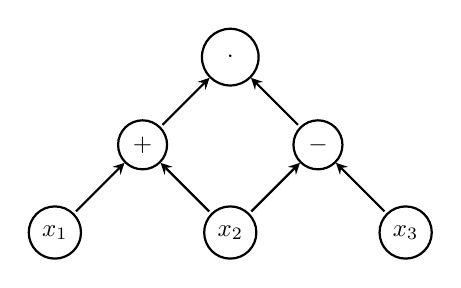
\begin{tikzpicture}[<-,>=stealth,shorten >=1pt,auto,node distance=1.75cm, thick,main node/.style={scale=0.9,circle,draw,font=\sffamily\normalsize}]

            \node[main node, minimum width=8mm, minimum height=8mm] (2) []{$\cdot$};
            \node[main node] (3) [below left of = 2]{$+$};
            \node[main node] (4) [below right of = 2]{$-$};
            \node[main node] (5) [below left of = 3]{$x_1$};
            \node[main node] (6) [below right of = 3]{$x_2$};
            \node[main node] (7) [below right of = 4]{$x_3$};

            \path[every node/.style={font=\sffamily\small}]
                (2) edge (3)
                (2) edge (4)
                (3) edge (5)
                (3) edge (6)
                (4) edge (6)
                (4) edge (7)
            ;
        \end{tikzpicture}

        \caption{An algebraic circuit encoding the polynomial $(x_1 + x_2)(x_2 - x_3)$.}
    \end{figure}

    Formally, the problem is defined as $\mathrm{PIT} = \{\abk{P_1, P_2} \mid \forall x \in \{0,1\}^m \;\; P_1(x) = P_2(x)\}$. This representation allows us to express polynomials in a very compact way. Many other problems in complexity theory are represented through circuits, such as the \textit{polynomial pigeonhole principle} or the \textit{polynomial parity argument}. The idea behind these problems is that we are \curlyquotes{forced} to avoid known simple algorithms since we're working with objects of exponential size with respect to the real input.
    
    For instance, given two polynomials $p$ and $q$, we could easily check if they are equal by first expanding until they reach the standard form $a_0 + a_1x_1 + \ldots + a_nx_n$ and then check if $p - q = 0$. This procedure clearly requires polynomial time with respect to the size of the polynomial. However, by expanding the polynomial represented by an algebraic circuit we get a polynomial of exponential size with respect to the input length (remember that the circuits are the input in $\mathrm{PIT}$). Hence, if we apply the previous procedure to $\mathrm{PIT}$, we get an exponential running time. Moreover, the expansion procedure alone clearly requires exponential time. These constraints make $\mathrm{PIT}$ not so trivial.

    However, this problem can be solved through randomization by reducing it to another $\mathsf{coRP}$ problem, i.e. the \textit{zero polynomial} problem. This new problem takes an algebraic circuit as input and asks to determine if the circuit represents the zero polynomial. Formally, we have that $\mathrm{ZEROP} = \{\abk{P} \mid \forall x \in \{0,1\}^m \;\; P(x) = 0\}$. The reduction from $\mathrm{PIT}$ to $\mathrm{ZEROP}$ is immediate: given the two input circuits $P_1, P_2$, we construct a new circuit $P = P_1 - P_2$ by joining them with a single gate. Vice versa, we can also reduce $\mathrm{ZEROP}$ to $\mathrm{PIT}$: given the input circuit $P$, we test if it is equal to a circuit that represents the zero polynomial. This makes the two problems completely equivalent. The proof of $\mathrm{ZEROP}$ lying inside $\mathsf{coRP}$ is based on a special case of the Schwartz-Zippel lemma, which we won't prove.

    \begin{framedlem}{Schwartz-Zippel lemma}
        Let $p \in \Z[x_1, \ldots, x_m]$ be a non-zero polynomial with total degree at most $d$ and let $S$ be a finite set of integers. Given $a_1,\ldots, a_m$ randomly chosen from $S$ (with replacement), it holds that:
        \[\Pr[p(a_1, \ldots, a_m) \neq 0] \geq 1 - \frac{d}{\abs{S}}\]
    \end{framedlem}

    Here, The total degree of a monomial $x^{d_1} \cdot \ldots \cdot x^{d_m}$ is equal to $d_1 + \ldots + d_m$. The total degree of a polynomial is the largest total degree of its monomials.

    \begin{framedthm}{}
        $\mathrm{ZEROP}$ and $\mathrm{PIT}$ are in $\mathsf{coRP}$
    \end{framedthm}

    \begin{proof}
        Let $P$ be a circuit representing a polynomial over $\Z[x_1, \ldots, x_m]$. We notice that a depth $d$ circuit contains at most $d$ multiplications, so it defines a polynomial of degree at most $2^d$ -- think of the circuit made of $d$ multiplication gates where the inputs of each gate are both the output of the previous gate.

        We can easily define the following probabilistic algorithm: choose $m$ numbers $a_1, \ldots, a_m$ from $S = \{1, \ldots, 10 \cdot 2^d\}$, evaluate $P(a_1, \ldots, a_m) = y$, accept if $y = 0$ and reject otherwise. We notice that the $m$ random numbers require $O(m \log 2^d) = O(md)$ random bits, thus they can be generated in polynomial time. If the input circuit $P$ represents the zero polynomial, the output will clearly always be correct. Otherwise, the Schwartz-Zippel lemma ensures that the probability of a wrong answer is low enough.

        However, the previous algorithm has a catch: the values that arise during the evaluation of $P(a_1, \ldots, a_m) = y$ may be require even $(10 \cdot 2^d)^{2^d}$ bits, making it impossible to compute in polynomial time. To fix this problem, we use a technique called \textit{fingerprinting}: we choose a random value $k \in [2^{2d}]$ and evaluate $P(a_1, \ldots, a_m) \equiv y \pmod{k}$. Clearly, if $y = 0$ then $y \equiv 0 \pmod{k}$, hence we still always accept when $P$ represents the zero polynomial. When $y \neq 0$, instead, we claim the following.

        \textbf{Claim}: If $y \neq 0$, with probability at least $\frac{1}{4d}$ a random $k \in [2^{2d}]$ doesn't divide $y$.

        \begin{proof}[Proof of the claim]
            Let $B = \{p_1, \ldots, p_t\}$ be the set of distinct prime factors of $y$. By the Prime Number Theorem, for sufficiently large $d$ we have that the number of primes in $[2^{2d}]$ is at least $\frac{2^{2d}}{\log 2^{2d}} = \frac{2^{2d}}{2d}$.

            Since $y$ can have at most $\log y \leq 5d2^d = o\rbk{\frac{2^{2d}}{2d}}$ prime factors, for sufficiently large values of $d$, the number of primes in $[2^{2d}] - B$ is at least $\frac{2^{2d}}{4d}$, thus a random $k \in [2^{2d}]$ will have this property with probability at least $\frac{1}{4d}$.
        \end{proof}

        Through this claim, we can choose a constant number of values $k_1, \ldots, k_h$ to boost the probability: we compute $P(a_1, \ldots, a_m) \equiv y_1 \pmod{k_i}$ for each $k_i$ and accept only when all the outputs $y_1, \ldots, y_h$ are equal to zero and reject otherwise. Hence, we get that $\mathrm{ZEROP} \in \mathsf{coRP}$ and by consequence that $\mathrm{PIT} \in \mathsf{coRP}$ through the previous reduction.

    \end{proof}

    
    \section{Zero-sided error and the class \textsf{ZPP}}

    Last but not least, we define a class based on \curlyquotes{zero-sided error}. The idea here is that when a machine cannot be $100\%$ sure if a string is in the language or not, it is allowed to output \curlyquotes{I don't know}, i.e. the symbol \curlyquotes{\,?\,}. This allows us to remove error from the computation for the price of \textit{uncertainty}. Of course, we have to keep the number of \curlyquotes{\,?\,} outputs low, otherwise every existing language would trivially be inside this class: we could just output \curlyquotes{\,?\,} for all the strings of the language. To define the \textbf{zero-error probabilistic polynomial time} class, we will directly use a definition based on random verifiability due to it being simpler.

    \begin{frameddefn}{The class $\mathsf{ZPP}$}
        We define $\mathsf{ZPP}$ as the class of languages for which there is a polynomial time \textsf{PTM} $M$ such that:
        \begin{itemize}
            \item If $\forall r \in \{0,1\}^*$ we have that $M(x,r) = 1$ then $x \in L$
            \item If $\forall r \in \{0,1\}^*$ we have that $M(x,r) = 0$ then $x \notin L$
            \item The general probability of a \curlyquotes{\,?\,} output is low:
            \[\forall x \in \{0,1\}^* \;\; \Pr_{r \in_{R} \{0,1\}^*}[M(x,r) = \,?] \leq \frac{1}{2}\]
        \end{itemize}
    \end{frameddefn}

    \newpage

    First of all, it's easy to see that $\mathsf{P} \subseteq \mathsf{ZPP}$ since any deterministic \TM here would output \curlyquotes{\,?\,} with zero probability. Moreover, a good eye may notice that $\mathsf{ZPP} = \mathsf{RP} \cap \mathsf{coRP}$, a fact that fully expresses the idea of \curlyquotes{zero-sided error}.

    \begin{framedthm}{The class $\mathsf{ZPP}$ (2nd Definition)}
        $\mathsf{ZPP} = \mathsf{RP} \cap \mathsf{coRP}$
    \end{framedthm}
    
    \begin{proof}
        If a language is in $\mathsf{ZPP}$ then every time the output of the machine is \curlyquotes{\,?\,} we can convert it into a 0, making the machine valid for $\mathsf{RP}$. Since $\mathsf{ZPP} \subseteq \mathsf{RP}$, we get that $\mathsf{coZPP} \subseteq \mathsf{coRP}$, but the class $\mathsf{ZPP}$ is actually closed under complement (it follows from the definition), thus $\mathsf{ZPP} \subseteq \mathsf{coRP}$ is also true. 
        
        Vice versa, if a language is in $\mathsf{RP} \cap \mathsf{coRP}$, we can simultaneously run the two machines $M$ and $M'$ that assert the membership of $L$ in $\mathsf{RP}$ and $\mathsf{coRP}$. We define a new machine $M''$ that runs both machine. If $M$ returns 1 and $M'$ returns 0, we output 1. Likewise, if $M$ returns 0 and $M'$ returns 1, we output 0. Otherwise, if the two machines give the same output, $M''$ returns \curlyquotes{\,?\,}.
    \end{proof}

    The presence of a \curlyquotes{\,?\,} output is mostly \curlyquotes{unwanted} since it makes reasoning about computation harder. Thankfully, we can remove this type of output through another way more convenient -- and actually very surprising -- definition.

    \begin{framedthm}{The class $\mathsf{ZPP}$ (3rd Definition)}
        Given a language $L$, it holds that $L \in \mathsf{ZPP}$ if and only if there is a polynomial $p$ and a \textsf{PTM} $M$ such that $\forall x \in \{0,1\}^*$ it holds that $M(x) = L(x)$ and:
        \[\forall x \in \{0,1\}^* \;\;\Exp[T_{M,x}] \leq p(\abs{x})\]
        where $T_{M,x}$ is the random variable describing the running time of $M(x)$. In other words, the expected runtime of $M$ is at most polynomial. The machine $M$ is often referred to as a \textbf{Las Vegas machine}.
    \end{framedthm}

    \begin{proof}
        Let $M$ be the \textsf{PTM} machine for which $L \in \mathsf{ZPP}$. Let $q$ be the polynomial describing the running time of $M$. We define a new machine $M'$ that repeatedly runs $M$ until it outputs 0 or 1. $X_{M,x}$ be the variable denoting the number of times $M(x)$ gets run inside $M'$, implying that $\Pr[X_{M',x} = i] \leq \frac{1}{2^{i-1}}$.Since every run requires $q(\abs{x})$ steps, we get that:
        \[\Exp[T_{M',x}] = \Exp[q(\abs{x}) \cdot X_{M',x}] = q(\abs{x}) \sum_{i = 0}^{+\infty} i \cdot \Pr[X_{M',x} = i] \leq q(\abs{x})  \sum_{i = 1}^{+\infty} \frac{i}{2^{i-1}} = 4q(\abs{x})\]
        hence the expected runtime of $M'$ is polynomially bounded.

        Vice versa, suppose that there is a Las Vegas machine $M$ for a language $L$, where $p$ is the polynomial that bounds the expected runtime. We define a new \textsf{PTM} $M'$ as follows. $M'$ runs $M$ for at least $k$ times its expected running time. If under $k \cdot \Exp[T_{M,x}]$ steps one of the executions gives an answer, $M'$ returns that answer. Otherwise, $M'$ outputs \curlyquotes{\;?\;}.

        Since $T_{M,x}$ is a non-negative random variable with a finite expected value, by Markov's inequality we have that:
        \[\Pr[T_{M',x} \geq k \cdot \Exp[T_{M',x}]] \leq \frac{1}{k}\]

        Hence, by choosing a nice value for $k$ -- say 100 -- we get that the probability of $M$ halting under $100 \cdot \Exp[T_{M',x}]$ inside $M'$ is greater than $1-\frac{1}{100}$. Thus, $M'$ returns \curlyquotes{\;?\;} with probability at most $\frac{1}{100}$.
    \end{proof}
    
    While reasoning about this new definition, we can with most certainty conclude that if a problem is inside $\mathsf{ZPP}$ then we're pretty much fine: we're now allowed to use randomness in order to perfectly decide a language, with the cost of getting a bad runtime in some cases. In fact, Las Vegas algorithms are often better than normal decision algorithms -- consider what we showed for the $\mathrm{MEDIUM}$ search problem.

    \section{Randomness, circuits and $\mathsf{PH}$}

    In the previous sections we discussed the relationships between probabilistic classes, $\mathsf{P}$, $\mathsf{NP}$ and $\mathsf{coNP}$. We also discussed how researchers believe that $\mathsf{P} \neq \mathsf{NP}$ and $\mathsf{P} = \mathsf{BPP}$ -- and consequently that all the probabilistic classes collapse into $\mathsf{P}$. We'll now prove two results \cite{adleman, sipser_bpp, lautemann_bpp} that show us how randomness is not a sufficient alternative to non-determinism.

    \begin{framedthm}{Adleman's theorem}
        $\mathsf{BPP} \subseteq \mathsf{P_{/poly}}$
    \end{framedthm}

    \begin{proof}
        Given a language $L \in \mathsf{BPP}$, let $M$ be the polynomial time $\mathsf{PTM}$ with boosted probability such that:
        \[x \in L \iff \Pr_{r \in_{R} \{0,1\}^*}[M(x,r) = L(x)] > 1-\frac{1}{2^{n+1}}\] 

        Through a probabilistic argument, we notice that, given a random string, the probability of this string being \textit{good} for all inputs is is given by:
        \[\begin{split}
            \Pr_{r \in_R \{0,1\}^*} [\forall x \in \{0,1\}^n \; M(x,r) = L(x)] & = 1 - \Pr_{r \in_R \{0,1\}^*} [\exists x \in \{0,1\}^n \; M(x,r) \neq L(x)] \\
            &=  1 - \Pr_{r \in_R \{0,1\}^*} \sbk{\bigcup_{x \in \{0,1\}^n} M(x,r) \neq L(x)}
        \end{split}\]

        Using the union bound, we have that:
        \[\begin{split}
            1 - \Pr_{r \in_R \{0,1\}^*} \sbk{\bigcup_{x \in \{0,1\}^n} M(x,r) \neq L(x)} & \geq 1 - \sum_{x \in \{0,1\}^n} \Pr_{r \in_R \{0,1\}^*} [M(x,r) \neq L(x)] \\
            & = 1 - \frac{2^n}{2^{n+1}} \\
            & = \frac{1}{2}
        \end{split}\]

        Hence, we conclude that, for any $n \in \N$, at least half of the random string must be good for all inputs $x \in \{0,1\}^n$. We call these strings \textit{perfect} for $n$. Then, for each $n \in \N$, we can fix a perfect string $r_n \in \{0,1\}^{p(n)}$ and use it as advice bits that can be given as additional inputs to an advice-taking \TM, concluding that $L \in \mathsf{P_{/poly}}$.
    \end{proof}

    Together with \nameref{karp_lipton}, the previous result implies that we cannot hope to find a randomized polynomial time algorithm that solves $\mathsf{NP}$-Complete problems. For instance, if we could solve $\mathrm{3SAT}$ in randomized polynomial time, then we would get that $\mathsf{NP} \subseteq \mathsf{BPP}$. Hence, we would also get that $\mathsf{NP} \subseteq \mathsf{P_{/poly}}$, which also implies that $\mathsf{PH} = \Sigma_2^P$, which is conjectured to be false. This leaves us with only one option: maybe it holds that $\mathsf{BPP} \subseteq \mathsf{NP}$ and $\mathsf{BPP} \subseteq \mathsf{P_{/poly}}$ but $\mathsf{NP} \not\subseteq \mathsf{P_{/poly}}$, meaning that randomness is too weak. There are no current conjectures for the inclusion between $\mathsf{BPP}$ and $\mathsf{NP}$.

    \begin{framedthm}[label=sips_gacs]{The Sipser-Gács-Lautemann theorem}
        $\mathsf{BPP} \subseteq \Sigma_2^P \cap \Pi_2^P$
    \end{framedthm}

    \begin{proof}
        Since $\mathsf{BPP}$ is closed under complement and $\Pi_2^P = \mathsf{co}\Sigma_2^P$, it is sufficient to prove that $\mathsf{BPP} \subseteq \Sigma_2^P$ to also get $\mathsf{BPP} \subseteq \Pi_2^P$.

        As in the previous theorem, given a language $L \in \mathsf{BPP}$, let $M$ be the polynomial time $\mathsf{PTM}$ with boosted probability such that:
        \[x \in L \iff \Pr_{r \in_{R} \{0,1\}^*}[M'(x,r) = L(x)] > 1-\frac{1}{2^{n}}\] 

        For any $x \in \{0,1\}^n$, let $S_x = \{r \in \{0,1\}^m \mid M(x,r) = 1\}$. We observe that if $x \in L$ then $\abs{S_x} \geq \rbk{1-\frac{1}{2^n}} 2^m$, while if $x \notin L$ then $\abs{S_x} \leq \frac{2^m}{2^n}$, meaning that for each input this set is either very large or very small.

        Given a subset $S \subseteq \{0,1\}^m$ and a string $u \in \{0,1\}^m$, we denote with $S\oplus u$ the set given by the \curlyquotes{bitwise XOR} of $S$ with $u$, that is $S \oplus u = \{x \oplus u \mid x \in S\}$. Let $k = \ceil{\frac{m}{n}}+1$. We claim the following two statements.

        \textbf{Claim 1}: For sufficiently large $n$, for every subset $S \subseteq \{0,1\}^m$ with $\abs{S} \leq \frac{2^m}{2^n}$ and every $k$ strings $u_1, \ldots, u_k \in \{0,1\}^m$, it holds that $\bigcup_{i = 1}^k (S \oplus u_i) \neq \{0,1\}^m$.

        \begin{proof}[Proof of the first claim]
            Since $\abs{S \oplus u_i} = \abs{S}$ by definition, we have that
            \[\abs{\bigcup_{i = 1}^k (S \oplus u_i)} \leq k \abs{S} \leq k \frac{2^m}{2^n}\]

            For a sufficiently large $n$, we get that $k \frac{2^m}{2^n} < 2^m$, concluding that the union cannot cover the whole set
        \end{proof}

        \textbf{Claim 2}: For sufficiently large $n$ and for every subset $S \subseteq \{0,1\}^m$ with $\abs{S} \geq \rbk{1-\frac{1}{2^n}} 2^m$, there exist $k$ strings $u_1, \ldots, u_k \in \{0,1\}^m$ such that $\bigcup_{i = 1}^k (S \oplus u_i) = \{0,1\}^m$.

        \begin{proof}[Proof of the second claim]

            We want to prove that the probability of the existence of such $k$ strings is greater than 0. Suppose that $u_1, \ldots, u_k$ are chosen independently at random from $\{0,1\}^m$. Let $B_r$ denote the even $r \notin \bigcup_{i = 1}^k (S \oplus u_i)$. By extension, for each $i \in [k]$ let $B_r^i$ denote the event $r \notin S \oplus u_i$. First, we notice that, by properties of the bitwise XOR, it holds that $r \notin S \oplus u_i$ if and only if $r \oplus u_i \notin S$. However, since $r \oplus u_i \in \{0,1\}^m$ and $\abs{S} \geq \rbk{1-\frac{1}{2^n}} 2^m$, it holds that $Pr[r \oplus u_i \notin S] < \frac{1}{2^n}$.

            Since $u_1, \ldots, u_k$ are independent from each other, we know that $\Pr[B_r^i] = \Pr[B_r^j]$ for all $i,j \in [k]$. Moreover, since $B_r = \bigwedge_{i = 1}^k B_r^i$, we get that $\Pr[B_r] = (\Pr[B_r^i])^k < \frac{1}{2^{nk}}$

            For a sufficiently large $n$, we get that $\frac{1}{2^{nk}} < \frac{1}{2^m}$. Since for every $r \in \{0,1\}^m$ we have that $\Pr[B_r] <  \frac{1}{2^m}$, the probability of the existence of a random string $r' \in \{0,1\}^m$ such that $B_r$ is true is less than 1, i.e. $\Pr[\exists r' \in \{0,1\} \;\; B_{r'}] < 1$

            This concludes that $\Pr[\exists u_1, \ldots, u_k \in \{0,1\}^m \;\; \bigcup_{i = 1}^k (S \oplus u_i) = \{0,1\}^m] > 0$
        \end{proof}

        Thanks to the two claims, we get that:
        \[x \in L \iff \exists \abk{u_1, \ldots, u_k}\in \{0,1\}^{O(mk)} \forall r \in \{0,1\}^m \; r \in \bigcup_{i = 1}^k (S_x \oplus u_i)\]

        which is equivalent to:
        \[x \in L \iff \exists \abk{u_1, \ldots, u_k} \in \{0,1\}^{O(mk)} \; \forall r \in \{0,1\}^m \;\; \bigvee_{i = 1}^k M(x, r \oplus u_i) = 1\]

        concluding that $L \in \Sigma_2^P$.
    \end{proof}

    Together with the Adleman's theorem, this result suggests that $\mathsf{BBP}$ may indeed lie inside $\mathsf{NP}$, giving us more insight on how $\mathsf{BPP} = \mathsf{P}$ might be true. In fact, every single property that is true for $\mathsf{P}$ seems to also be true for $\mathsf{BPP}$.

    \begin{figure}[H]
        \centering

        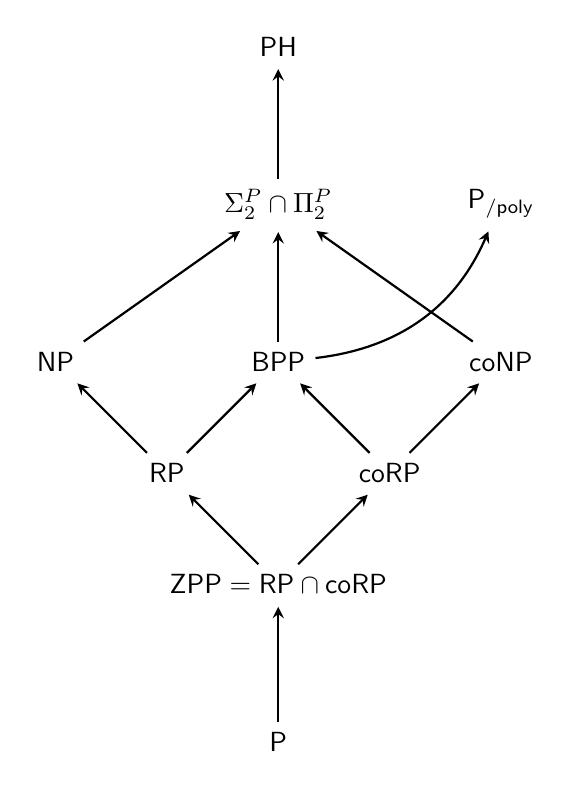
\begin{tikzpicture}[->,>=stealth,shorten >=1pt,auto,node distance=2cm,thick,main node/.style={scale=0.8,circle,draw,font=\sffamily\normalsize}]
            \node[] (1) []{$\mathsf{P}$};

            \node[] (2) [above of = 1]{$\mathsf{ZPP} = \mathsf{RP} \cap \mathsf{coRP}$};

            \node[] (3) [above left of = 2]{$\mathsf{RP}$};
            \node[] (4) [above right of = 2]{$\mathsf{coRP}$};

            \node[] (5) [above left of = 3]{$\mathsf{NP}$};
            \node[] (6) [above right of = 3]{$\mathsf{BPP}$};
            \node[] (7) [above right of = 4]{$\mathsf{coNP}$};

            \node[] (8) [above of = 6]{$\Sigma_2^P \cap \Pi_2^P$};
            
            \node[] (9) [above of = 8]{$\mathsf{PH}$};

            \node[] (10) [above of = 7]{$\mathsf{P_{/poly}}$};

            \path[every node/.style={font=\sffamily\small}]
                (1) edge (2)
                (2) edge (3)
                (2) edge (4)
                (3) edge (5)
                (3) edge (6)
                (4) edge (6)
                (4) edge (7)
                (5) edge (8)
                (6) edge (8)
                (7) edge (8)
                (8) edge (9)
                (6) edge[bend right] (10)
                ;
        \end{tikzpicture}

        \caption{Summary of the class inclusions discussed in this chapter}
    \end{figure}

    \addtocontents{toc}{\protect\newpage}
    \chapter{Space complexity}

    \section{Relations between time and space}

    In the previous chapters we have focused on the running time of Turing machines, while the \textbf{space requirements} have been neglected. Generally, time complexity is considered more important than space complexity, even though the latter is also a fundamental topic in computation. In particular, we will show that this type of complexity is highly related with \textit{games}.

    We recall that the \textit{required space} $S(n)$ of a Turing machine $M$ the number of tape cells written by the heads during the computation for an input of length $n$, except the input tape's cells. While working with decision problems, we can also omit the space complexity of the output tape, since only 1 bit is required for the output. Thus, for decision problems we consider only the cells written on the \textbf{work tape}. The classes $\mathrm{DSPACE}$ and $\mathrm{NSPACE}$ follow the same definition of $\mathrm{DTIME}$ and $\mathrm{NTIME}$, where time is replaced by space.

    Just like the trivial inclusion $\mathrm{DTIME}(f(n)) \subseteq \mathrm{NTIME}(f(n))$, it also trivially holds that $\mathrm{DSPACE}(f(n)) \subseteq \mathrm{NSPACE}(f(n))$. We already mentioned how time easily limits space: if a machine $M$ runs in time $T(n)$ then it can write at most $T(n)$ cells, meaning that $S(n) \leq T(n)$. Thus, it clearly holds that $\mathrm{DTIME}(f(n)) \subseteq \mathrm{DSPACE}(f(n))$ and $\mathrm{NTIME}(f(n)) \subseteq \mathrm{NSPACE}(f(n))$.
    
    These last inclusions can be improved through a fundamental property that differentiates space complexity from time complexity: the possibility of \textbf{re-using space}, i.e. using cells that were previously written without writing new ones. This property makes space complexity way more powerful than time complexity: since we don't care about time, we could make an exponential number of steps even in a very low amount of space. In fact, deterministic space machines are even stronger even than non-deterministic time ones.

    \begin{framedprop}[label=time_lim_space]{Space bounded by time}
        For any time-constructible function $T : \N \to \N$, it holds that:
        \[\mathrm{DTIME}(f(n)) \subseteq \mathrm{NTIME}(f(n)) \subseteq \mathrm{DSPACE}(f(n))\]
    \end{framedprop}

    \begin{proof}
        Let $V$ be a verifier for a language $L$ with running time $R(n)$. Since $V$ runs in $T(n)$ steps, we know that the length of each witness will be at most $T(n)$. We define a new machine $M$ as follows: given the input string $x$, cycle between all the possible strings $w \in \{0,1\}^{T(n)}$ and check if $V(x,w) = 1$. If $V$ accepts then $M$ also accepts. If none of the possible strings are a valid witness, $M$ rejects.
        
        The running time of $M$ is clearly $O(2^{T(n)})$, but we only care about space. Each witness has length at most $T(n)$, while $V$'s simulation requires at most $T(n)$ cells. On each iteration, we can reuse the cells of the previous iteration, concluding that we require at most $O(T(n))$ space and thus that $L \in \mathrm{DSPACE}(T(n))$.  
    \end{proof}

    Space can also limit time, even though this bound is not as powerful as the one imposed by time on space. To achieve this limitation, we use the notion of \textbf{configuration graph}. Let $M$ be a deterministic (or non-deterministic) \TM. A \textit{configuration} of $M$ is a string containing of all non-blank entries of $M$'s work tape, along with its state and head positions, at a particular point in its execution. For instance, the encoding $\mathtt{WORKT\underline{A}PE};j;q_i$ represents a configuration such that:
    \begin{itemize}
        \item The work tape contains the string $\mathtt{WORKTAPE}$
        \item The work tape's head is positioned on the cell $\mathrm{A}$
        \item The input tape's head is positioned on the $j$-th cell
        \item The current state is $q_i$
    \end{itemize}

    \begin{frameddefn}{Configuration graph of a computation}
        Let $M$ be a \TM (or $\mathsf{NDTM}$) and let $x$ an input. The \textbf{configuration graph} of the computation $M(x)$ is the directed graph $G_{M,x}$ whose nodes are all the possible configurations of $M$, where two nodes $C_i, C_j$ are connected by a directed edge if $M$ can transition from $C_i$ to $C_j$ when the input is $x$, according to its transition function. The node corresponding to the initial configuration is $C_{\mathrm{start}}$. Since $G_{M,x}$ may have more than one accepting configuration, to ensure that we have only one final node, we add an additional node $C_{\mathrm{accept}}$ whose in-going edges come only from all the accepting configurations.
    \end{frameddefn}

    By definition, for each pair of inputs $x,x'$ the graphs $G_{M,x}$ and $G_{M,x'}$ will have the same set of nodes. However, their edges may be different. The configuration graph of a computation allows us to convert the computation $M(x)$ to a simple graph problem: we have that $M(x) = 1$ if and only if $G_{M,x}$ has a path from $C_{\mathrm{start}}$ to $C_{\mathsf{accept}}$.

    \begin{framedprop}[label=space_lim_time]{Time bounded by space}
        For any space-constructible function $f : \N \to \N$ with $f(n) \geq \log n$, it holds that:
        \[\mathrm{DSPACE}(f(n)) \subseteq \mathrm{NSPACE}(f(n)) \subseteq \mathrm{DTIME}(2^{f(n)})\]
    \end{framedprop}

    \begin{proof}
        First, we notice that if $M$ is deterministic, then the graph $G_{M,x}$ has out-degree one, while if $M$ is non-deterministic then the graph has out-degree
        at most two. Thus, non-determinism doesn't really change the graph size, only the number of edges, which can still be at most the square of the number of vertices.

        If the space complexity of $M$ is $S(n)$, then each configuration requires $O(S(n))$ bits to be encoded. This implies that there are at most $2^{O(S(n))}$ configurations, meaning that the graph has exponential size. We can define a machine $M'$ that, given the input $x$, first constructs the graph $G_{M,x}$ and then runs a DFS on such graph to find a path from $C_{\mathrm{start}}$ to $C_{\mathsf{accept}}$. Since a DFS requires linear time with respect to the graph size, this computation requires at most $2^{O(S(n))}$ steps.
    \end{proof}   
    
    In the previous proof, we reasoned on how to use time by reasoning on space. However, a very similar idea can be used to work with space while reasoning on space itself. Through this intuition, \textcite{savitch} showed that deterministic space is even capable of simulating non-deterministic space with an small blow-up in required space.

    \begin{framedthm}[label=savitch_thm]{Savitch's theorem}
        For any space-constructible function $f : \N \to \N$ with $f(n) \geq \log n$, it holds that:
        \[\mathrm{NSPACE}(f(n)) \subseteq \mathrm{DSPACE}(f(n)^2)\]
    \end{framedthm}

    \begin{proof}
        Let $N$ be a \textsf{NDTM} with required space $S(n)$. For any input $x$, we know that the configuration graph $G_{N,x}$ has $2^{O(S(n))}$ nodes. We notice that that, for any vertices $u,v$, there is a path $u \to v$ of length at most $2^k$ if and only if there's a node $z$ with two paths $u \to z$ and $z \to y$ both of at most $2^{i-1}$ nodes. Based on this idea, we define the following deterministic recursive procedure that returns 1 if and only if there is a path $u \to v$ of length at most $2^k$.
        
        $\mathtt{Reach?}(G, x, y, k)$:
        \begin{enumerate}
            \item If $k = 0$, check if $x = y$. If true, return 1. Otherwise, return 0.
            \item If $k = 1$, check if $(x,y) \in E(G)$. If true, return 1. Otherwise, return 0.
            \item If $k > 0$, repeat the following for each node $z \in V(G)$:
            \begin{enumerate}[label={\arabic*.}, start=4]
                \item Recursively run $\mathrm{Reach?}(x, z, k-1)$ and $\mathrm{Reach?}(z, y, k-1)$. If they both return 1, then return 1. Otherwise, return 0.
            \end{enumerate}
        \end{enumerate}

        By defining a \TM $M$ that computes $\mathrm{Reach?}(G_{N,x}, C_{\mathrm{start}}, C_{\mathrm{accept}}, S(n))$ on input $x$, we get that $M(x) = 1$ if and only if there is a path of at most $2^{S(n)}$ nodes, which covers the whole graph.

        Now we focus on the space complexity of the procedure. Let $R(m, k)$ be the space complexity of the procedure while being run on a graph $G$ with $m$ nodes and a value $k$. We notice that on each recursive step, the procedure requires $\Theta(\log m)$ cells to enumerate all the vertices since -- assuming the nodes are also labeled by a number and not only by a configuration -- we only need to store the index of the current node. Moreover, while doing the second recursive call, the procedure can re-use the space of the first recursive call. We get that $R(m, k) = R(m, k-1) + \Theta(\log m)$, where $R(m, 0) = R(m, 1) = \Theta(1)$. By solving this recursive equation, we conclude that $R(m, k) = \Theta(k \log m)$.

        Thus, the computation of $\mathrm{Reach?}(G_{N,x}, C_{\mathrm{start}}, C_{\mathrm{accept}}, S(n))$ requires $O(S(n)^2)$ space. However, since the graph $G_{N,x}$ has exponential size, the space required by $M$ to compute the whole graph $G_{N,x}$ before running the procedure would be too large. To fix this issue, we can simply compute the nodes of the graph during the recursion: the next node to be iterated on is simply the next generate configuration.
    \end{proof}

    The same idea that we used in the \nameref{dtime_hier} also holds for the \textbf{Space Hierarchy Theorem}. However, in this case the deterministic space hierarchy theorem is actually stronger than the deterministic time hierarchy theorem. This is due to the possibility of re-using the same cells, preventing the logarithmic blow-up. Moreover, the same result holds for both the deterministic and non-deterministic versions of the theorem. In this context, the concept of space-constructible function follows the same idea of time-constructible functions: a function $S : \N \to \R^+$ is said to be \textbf{space-constructible} if there is a \TM $M$ that computes it using at most $S(n)$ cells for all $n \in \N$. 

    \begin{framedthm}{Space Hierarchy Theorem}
        For all functions $f, g : \N \to \N$ with $g$ space-constructible and $f(n) = o(g(n))$
        \[\mathrm{DSPACE}(f(n)) \subsetneq \mathrm{DSPACE}(g(n))\]
        \[\mathrm{NSPACE}(f(n)) \subsetneq \mathrm{NSPACE}(g(n))\]
    \end{framedthm}

    \begin{proof}
        Omitted.
    \end{proof}

    \newpage

    \section{Games and the class $\mathsf{PSPACE}$}
    
    After defining the relationships between time and space, we are ready to define the space complexity equivalents of $\mathsf{P}$ and $\mathsf{NP}$, i.e. the classes $\mathsf{PSPACE}$ and $\mathsf{NPSPACE}$

    \begin{frameddefn}{The classes $\mathsf{PSPACE}$ and $\mathsf{NPSPACE}$}
        We define $\mathsf{PSPACE}$ as the class of the languages decidable in polynomial space:
        \[\mathsf{PSPACE} = \bigcup_{k \geq 0} \mathrm{DSPACE}(n^k)\]

        Likewise, we define $\mathsf{NPSPACE}$ as the class of the languages decidable in non-deterministic polynomial space:
        \[\mathsf{NPSPACE} = \bigcup_{k \geq 0} \mathrm{NSPACE}(n^k)\]
    \end{frameddefn}


    \nameref{savitch_thm} directly concludes that $\mathsf{PSPACE} = \mathsf{NPSPACE}$, proving that space is indeed very different from time. This quite surprising since our intuition is that the corresponding classes for time complexity are separated. From \Cref{time_lim_space} and \Cref{space_lim_time}, instead, we easily get that:
    \[\mathsf{P} \subseteq \mathsf{NP} \subseteq \mathsf{PH} \subseteq \mathsf{PSPACE} \subseteq \mathsf{EXP} \subseteq \mathsf{NEXP}\]

    As for the class $\mathsf{NP}$, we're interested in defining a concept of $\mathsf{PSPACE}$-Hard. However, we have to make some clever observations. Since we defined $\mathsf{NP}$-Hardness through Karp reductions, i.e. polynomial time reductions, the simplest idea would be to define $\mathsf{PSPACE}$-Hardness through polynomial space reductions. However, we notice that, in this case, any single problem in $\mathsf{PSPACE}$ would also be $\mathsf{PSPACE}$-Complete: given two problems $A,B \in \mathsf{PSPACE}$, two inputs $x_\mathrm{yes},x_\mathrm{no}$ such that $x_\mathrm{yes} \in B$ and $x_\mathrm{no} \notin B$ and a poly-space machine $M$ that solves $A$, we can define a function $f$ such that $f(x) = x_{\mathrm{yes}}$ if $M(x) = 1$ and $f(x) = x_{\mathrm{no}}$ if $M(x) = 0$. Since the simulation of $M$ requires polynomial space, $f$ is a polynomial space reduction for which $x \in A$ iff $f(x) \in B$ -- notice that this \curlyquotes{trick} doesn't work for $\mathsf{NP}$-Completeness since the computation of $f$ \underline{must} be deterministic.

    In order to give a better definition of $\mathsf{PSPACE}$-Hardness, we have to look to the \textit{implications} of $\mathsf{NP}$-Complete: if any $\mathsf{NP}$-Complete problem is proven to be in $\mathsf{P}$, then the whole class $\mathsf{NP}$ collapses into $\mathsf{P}$. With this idea in mind, a more interesting definition of $\mathsf{PSPACE}$-Hardness derives from the preservation of Karp reductions.

    \begin{frameddefn}{$\mathsf{PSPACE}$-Hardness and $\mathsf{PSPACE}$-Completeness}
        A language $B$ is said to be $\mathsf{PSPACE}$-Hard if $\forall A \in \mathsf{PSPACE}$ it holds that $A \leq_P B$. If $B$ is also in $\mathsf{PSPACE}$, we say that it is $\mathsf{PSPACE}$-Complete.
    \end{frameddefn}

    This definition clearly preserves the idea of \curlyquotes{collapse under reductions}: if any $\mathsf{PSPACE}$-Complete problem is proven to be in $\mathsf{NP}$ (or $\mathsf{P}$), then the whole class $\mathsf{PSPACE}$ collapses into $\mathsf{NP}$ (or $\mathsf{P}$). The most interesting $\mathsf{PSPACE}$-Complete problem that satisfies this definition is the \textit{true quantified Boolean formula problem}, defined as follows:
    \[\mathrm{TQBF} = \{\abk{\psi} \mid \psi = [Q_1 x_1 \; \ldots \; Q_k x_k \; \phi(x_1, \ldots, x_k)] \text{ is true}\}\]
    where $\phi$ is an unquantified Boolean formula and $Q_1, \ldots, Q_k$ are either $\exists$ or $\forall$, without restrictions. We notice that since all the variables of a QBF are bound by some quantifier, the QBF is always either true or false. Moreover, we notice that this problem differs from $\Sigma_n^P\mathrm{SAT}$ and $\Pi_n^P\mathrm{SAT}$ for two reasons: the quantifiers don't have to be alternating and the whole quantified formula must be an always-true statement.

    We won't dive into the proof of $\mathsf{PSPACE}$-Completeness for this problem, but the idea is similar to what can be done for $\mathrm{SAT}$: just encode the whole computation as a QBF that is always true.

    \begin{framedthm}{}
        $\mathrm{TQBF}$ is $\mathsf{PSPACE}$-Complete
    \end{framedthm}

    \begin{proof} Omitted. \end{proof}

    We recall that the central feature of $\mathsf{NP}$ problems is that a yes answer has a short certificate. The analogous concept for $\mathsf{PSPACE}$ problems seems to be that of a \textbf{winning strategy for a two-player game} with perfect information. A good example of such a game is Chess: Two players alternately make moves, and the moves are made on a board visible to both, hence the term \textit{perfect information}. Here, a \textit{winning strategy} refers to a predefined set of moves that guarantees a player victory in a game, regardless of how the opponent plays. Clearly, any winning strategy can be represented as a QBF. There are $2k$ variables $x_1, \ldots, x_{2k}$ such that odd numbered variables correspond to the move of Player 1 and even numbered variables correspond to the move of Player 2.
    
    In order for Player 1 to have a winning strategy, they must have a way to win for all possible sequences of moves by Player 2. In other words, we have that:
    \[\exists x_1 \; \forall x_2 \; \exists x_3 \; \ldots \; \exists x_{2k-1} \; \forall x_{2k} \; \phi(x_1, \ldots, x_{2k}) \text{ is true}\]

    The same idea also holds for a winning strategy for Player 2: we just have to swap each $\exists$ with a $\forall$ and vice versa. Deciding whether or not a player has a winning strategy seems to require searching the tree of all possible moves. This looks like something we would do in $\mathsf{NP}$. However, just like in the case of the polynomial hierarchy, the crucial difference is the lack of a short witness for the statement “Player 1 has a winning strategy,” since the only certificate we can think of is the winning strategy itself, which requires exponentially many bits to even describe.

    In 1976, Tarjan and Even suggested that this difference between $\mathsf{NP}$ and $\mathsf{PSPACE}$ is the same as for why \textit{puzzles} are easier than \textit{games}, that is the fact that the initiative can shift back and forth between the players.

    Proving $\mathsf{PSPACE}$-Completeness of games may seem like a frivolous pursuit, but similar ideas lead to $\mathsf{PSPACE}$-Completeness of some practical problems. Usually, these problems involve repeated moves by an agent who faces an adversary with unlimited computational power. For instance, many computational problems of robotics involve a robot navigating in a changing environment.

    \section{Logarithmic space and the classes $\mathsf{L}, \mathsf{NL}$}

    In the context of time complexity, the running time of a machine clearly cannot be lower than the input length, since otherwise the machine wouldn't even be able to read the whole input. Thus $T(n) \geq n$ is always true. In space complexity, instead, the number of cells written on the work tape can be way lower than the length of the input string. However, we still require that the space is at least logarithmic,  since otherwise we wouldn't be able to achieve interesting computations. Thus, we assume that $S(n) \geq \log n$. We define the additional two classes based on \textbf{logarithmic space}.

    \begin{frameddefn}{The classes $\mathsf{L}$ and $\mathsf{NL}$}
        We define $\mathsf{L}$ as the class of the languages decidable in logarithmic space:
        \[\mathsf{L} = \mathrm{DSPACE}(\log n)\]

        Likewise, we define $\mathsf{NL}$ as the class of the languages decidable in non-deterministic logarithmic space:
        \[\mathsf{NL} = \mathrm{NSPACE}(\log n)\]
    \end{frameddefn}
    
    Clearly, we have that $\mathsf{L} \subseteq \mathsf{NL}$. Since $S(n) \geq \log n$ is assumed to always be true, any language that is in $\mathsf{L}$ (or $\mathsf{NL}$) can be computed in $\Theta(\log n)$. This makes low space a nice topic of study: many algorithms may have to be executed on devices with very limited memory. From \Cref{time_lim_space} and \Cref{space_lim_time}, we get that $\mathsf{L} \subseteq \mathsf{NL} \subseteq \mathrm{DTIME}(n) \subseteq \mathsf{P}$. This means that any low space computation requires at most linear time. This makes low space computation not only very efficient in space but also very efficient in time. \nameref{savitch_thm}, instead, shows that $\mathsf{NL} \subseteq \mathsf{L}^2$, where the latter is the class $\mathsf{L}^2 = \mathrm{DSPACE}(\log^2 n)$. Even thought space is more flexible than time, the question $\mathsf{L} \stackrel{?}{=} \mathsf{NL}$ is as-hard-as the question $\mathsf{P} \stackrel{?}{=} \mathsf{NP}$.

    Following the same argument that we made for $\mathsf{PSPACE}$-Completeness, in order to define $\mathsf{NL}$-Completeness we have to slightly tweak our definitions. In this particular case, we're trying to make the class $\mathsf{NL}$ collapse onto the class $\mathsf{L}$. Hence, we have to preserve logarithmic space. When $A$ reduces to $B$ in logarithmic space, we write $A \leq_L B$.

    \begin{frameddefn}{$\mathsf{NL}$-Hardness and $\mathsf{NL}$-Completeness}
        A language $B$ is said to be $\mathsf{NL}$-Hard if $\forall A \in \mathsf{NL}$ it holds that $A \leq_L B$. If $B$ is also in $\mathsf{NL}$, we say that it is $\mathsf{NL}$-Complete.
    \end{frameddefn}

    \newpage

    In Karp reductions, one of the main properties is the transitivity between reductions, that is the fact that if $A \leq_P B$ and $B \leq_P C$ then $A \leq_P C$. For logarithmic space reductions, this transitivity property still holds, but it isn't as trivial as the polynomial time case: a log-space machine might not even have the memory to write down its output. To solve this issue, we can compute the two reduction bit-by-bit: after computing the next bit of the first reduction, we feed this bit to the second reduction, producing the next final bit. This is similar to how in \Cref{savitch_thm} the graph gets generated during the recursive calls. This idea preserves the transitive property for log-space reductions, meaning that if $A \leq_L B$ and $B \leq_L C$ then $A \leq_L C$. With the same idea, we get that if $A \leq_L B$ and $B \in \mathsf{L}$ then $A \in \mathsf{L}$: we compute the reduction bit-by-bit and feed the result to $B$'s log-space machine.
    
    The main $\mathsf{NL}$-Complete problem is the \textit{st-connectivity problem}, i.e. the $\mathrm{PATH}$ problem that we already discussed. This shouldn't come as a surprise: \nameref{savitch_thm} essentially reduces any non-deterministic computation to a $\mathrm{PATH}$ instance. Again, the idea is to generate the graph $G_{N,x}$ bit-by-bit while feeding it to a machine that solves $\mathsf{PATH}$. This easily makes the problem $\mathsf{NL}$-Hard. To show that it also lies in $\mathsf{NL}$, we consider  a non-deterministic BFS: each branch has to store only the previous node, meaning that logarithmic space suffices.

    \begin{framedthm}{}
        $\mathrm{PATH}$ is $\mathsf{NL}$-Complete
    \end{framedthm}
    
    As for the class \NPclass, in \NLSPACE class we can also derive the alternative definition via verifier. However, in this case we need needs a small change in order to respect the strict space constraints:
    \begin{itemize}
        \item By constraining the witness to a logarithmic length we obtain a too restricted subset of problems, due to the witness being too small, therefore the subset of considered problems would not cover \NLSPACE
        \item By keeping the witness of polynomial length the witness can be used as \textit{additional memory}: we could read the same information multiple times without having to store it in the work tape, saving a considerable amount of space
    \end{itemize}

    In other words, in the first case we obtain verifiers that are too weak, while in the second they are too powerful. To get a middle ground between the two, we can impose that the witness has a polynomial length certificate that is \textbf{read-once}: the verifier has an additional tape containing the witness whose cells can be read only once -- in other words, the head cannot move to the left.

    \begin{framedthm}{The class \NLSPACE (2nd Definition)}
        Given the \NLSPACE class, we have that:
        \[\NLSPACE = \{L \subseteq \{0,1\}^* \mid L \text{ is verifiable by read-once witnesses in log space}\} \]
    \end{framedthm}

    \newpage

    This alternative definition of $\mathsf{NL}$ also gives us a nice alternative definition for the class $\mathsf{coNL}$. In particular, since $\mathrm{PATH}$ is $\mathsf{NL}$-Complete, we know that $\overline{\mathrm{PATH}}$ is $\mathsf{coNL}$-Complete. Unlike in the case of $\mathrm{PATH}$, there is no natural witness for the non-existence of a path between two nodes, thus it seemed \curlyquotes{obvious} to researchers that $\overline{\mathrm{PATH}} \notin \mathsf{NL}$. In two surprising results, \textcite{immerman, szelepcsenyi} showed that this intuition was wrong. As a corollary, this implies that the class $\mathsf{NL}$ is actually closed under complementation, i.e. that $\mathsf{NL} = \mathsf{coNL}$.

    \begin{framedthm}{The Immerman-Szelepcsényi theorem}
        $\overline{\mathrm{PATH}} \in \mathsf{NL}$
    \end{framedthm}

    \begin{proof}
        Let $m = \abs{V(G)}$ and let $R_0, \ldots, R_{m-1}$ be the sets of vertices reachable from $s$ with maximum $i \in [0,m-1]$ steps:
        \[R_i = \{v \in V(G) \mid s \to v \text{ with maximum $i$ edges}\}\]

        Let us also assume that the vertices of $G$ are identified by a number in $[0, m-1]$. This will be a \underline{key assumption}: the procedure must be valid for \textit{some} certificate, hence we can always assume that our certificate follows our idea. However, this also implies that we have to preserve our assumption by rejecting certificates that aren't based on this idea.

        The idea behind the following proof is that the polynomial length of the certificate can be abused: we cannot read the same cells multiple times, but we can insert an adequate number of copies of the same information. In particular, our input certificate will be a sequence of recursively defined sub-certificates. Our verifier will be based on four sub-procedures. Each call of these procedures will have a recursive input certificate. To give an intuition behind what we're trying to achieve, we'll start by defining the final verifier:
        
        $V$ = "Given the string $\abk{\abk{G,s,t}, c}$ as input:
        \begin{enumerate}[label={\arabic*.}]
            \item Check if $s \neq t$. If false, \textit{rejects}.
            \item Interpret $c = \abk{(\ell_1, c_1), \ldots, (\ell_{k}, c_k),c_t}$
            \item Set $\mathrm{prev} = 1$
            \Comment $\ell_0$ is equal to 1
            \item Set $i = 1$ and repeat while $i \leq k$:
            \begin{enumerate}[label={\arabic*.}, start=5]
                \item Set $\mathrm{curr} = \ell_i$
                \item Execute the sub-procedure $\mathtt{certify\_\abs{R_{i}}\_with\_\abs{R_{i-1}}\,}(i, \mathrm{curr}, c_i, \mathrm{prev},)$. If the sub-procedure rejects, $V$ \textit{rejects} too.
                \item Set $\mathrm{prev} = \mathrm{curr}$.
            \end{enumerate}
        \end{enumerate}
        \begin{enumerate}[label={\arabic*.}, start=8]
            \item Check if $k = m-1$. If false, \textit{reject}.
            \item Execute the sub-procedure $\mathtt{certify\_v\_not\_in\_R_i\_with\_\abs{R_{i}}\,}(m, t, c_t, \mathrm{curr})$. If the sub-procedure accepts, $V$ also \textit{accepts}. Otherwise $V$ \textit{rejects}.
        \end{enumerate}

        Here, each input $\ell_i$ is an integer value that is verified by the sub-certificate $c_i$: the procedure $\mathtt{certify\_\abs{R_{i}}\_with\_\abs{R_{i-1}}}$ verifies that $\abs{R_i} = \ell_i$ using the previously verified value $\ell_{i-1}$. In other words, the values $\ell_0, \ldots, \ell_m$ are used to inductively verify each other. In particular, we notice that $\abs{R_0} = \ell_0 = 1$ is always true since $R_0 = \{s\}$. After verifying that $\abs{R_m} = \ell_m$, the procedure $\mathtt{certify\_v\_not\_in\_R_i\_with\_\abs{R_{i}}}$ will verify if $t \notin R_n$ is true. When this holds, we can conclude that there is no path from $s$ to $t$. We also notice that, thanks to the stored values, each cell of the input certificate is read once. 
        
        For now, we focus on the last procedure, which uses a sub-certificate to witness the membership of $\abs{R_i}$ different nodes in the set $R_i$. If all of these nodes are different from the input node $v$ then we can conclude that $v \notin R_i$.

        $\mathtt{certify\_v\_not\_in\_R_i\_with\_\abs{R_{i}}\,}\rbk{i, v, \abk{c_{u_{1}}, \ldots, c_{u_{{k}}}}, \ell_i}$:

        \begin{enumerate}[label={\arabic*.}]
            \item Set $i' = i$
            \item Set $v' = v$
            \item Set $\mathrm{prev} = -\infty$.
            \item Set $h = 1$ and repeat while $h \leq k$:
            \begin{enumerate}[label={\arabic*.}, start=3]
                \item Set $\mathrm{curr} = u_h$
                \item Check if $\mathrm{curr} \neq v'$. If false, \textit{reject}.
                \item Check if $\mathrm{prev} < \mathrm{curr}$. If false, \textit{reject}.
                \item Check if $\mathrm{next} \in R_i$ using the sub-procedure $\mathtt{certify\_v\_in\_R_i\,}(c_{\mathrm{curr}}, i', \mathrm{curr})$. If the sub-procedure rejects, this procedure \textit{rejects} as well.
                \item Set $\mathrm{prev} = \mathrm{curr}$.
                \item Increment $h$ by 1.
            \end{enumerate}
        \end{enumerate}
        \begin{enumerate}[label={\arabic*.}, start=6]
            \item Check if $h = \ell_i$. If true, \textit{accept}, otherwise \textit{rejects}.
        \end{enumerate}

        Each sub-certificate $c_{u_k}$ is used to witness that $u_k \in R_i$. The check $\mathrm{prev} < \mathrm{curr}$ ensures that the certificate that we're working with respects our assumption. In particular, this allows us to use transitivity to ensure that all the nodes being witnessed are different from each other.

        For each vertex $v \in V(G)$, verifying that $v \in R_i$ holds is very easy: all it takes is a single certificate $\abk{u_1, \ldots u_k}$ describing a path from $s$ to $v$ with at most $i$ edges. We notice that, since $u_1, \ldots, u_k$ are not sub-certificates, this procedure is a leaf of the recursive verification procedure.

        $\mathtt{certify\_v\_in\_R_i\,}(v, \abk{u_1, \ldots, u_k}, i)$:

        \begin{enumerate}[label={\arabic*.}]
            \item Set $v' = v$.
            \item Set $\mathrm{prev} = u_1$.
            \item Check if $\mathrm{prev} \neq v'$. If false, \textit{reject}.
            \item Set $h = 2$ and repeat while $h \leq k$:
            \begin{enumerate}[label={\arabic*.}, start=5]
                \item Set $\mathrm{curr} = u_h$
                \item If $h \neq k$, check if $\mathrm{curr} \neq v'$. If false, \textit{reject}.
                \item If $h = k$, check if $\mathrm{curr} = v'$. If false, \textit{reject}.
                \item Check if $\mathrm{prev} < \mathrm{curr}$. If false, \textit{reject}.
                \item Check if $(\mathrm{prev}, \mathrm{curr}) \in E(G)$. If false, \textit{reject}
                \item Set $\mathrm{prev} = \mathrm{curr}$.
                \item Increment $h$ by 1.
            \end{enumerate}
        \end{enumerate}
        \begin{enumerate}[label={\arabic*.}, start=11]
            \item Check if $h \leq i$ and $\mathrm{curr}$. If true, \textit{accept}, otherwise \textit{rejects}.
        \end{enumerate}

        We now move to the procedure $\mathtt{certify\_\abs{R_{i}}\_with\_\abs{R_{i-1}}}$. This procedure will check that each node witnessed by its sub-certificate is inside $R_i$, where the expected number of nodes in $\ell_i$. In particular, for each node $u_h$ we will have to rune two sub-procedures. First, we check if $u_h \in R_i$. If false, we also check if $u_h \notin R_i$ using $\mathrm{R_{i-1}}$. This second check is necessary: the first procedure may also reject when the certificate has the wrong expected format.

        $\mathtt{certify\_\abs{R_{i}}\_with\_\abs{R_{i-1}}}\rbk{i, {\ell_{i-1}}, \abk{c_{u_{1}}, \ldots, c_{u_{{k}}}}, \ell_{i}, }$:

        \begin{enumerate}[label={\arabic*.}]
            \item Set $i' = i$
            \item Set $\ell_{i-1}' = \ell_{i-1}$
            \item Set $v' = v$
            \item Set $\mathrm{prev} = -\infty$.
            \item Set $h = 1, q = 1$ and repeat while $h \leq k$:
            \begin{enumerate}[label={\arabic*.}, start=3]
                \item Set $\mathrm{curr} = u_h$
                \item Check if $\mathrm{prev} < \mathrm{curr}$. If false, \textit{reject}.
                \item Check if $\mathrm{curr} \in R_i$ using the sub-procedure $\mathtt{certify\_v\_in\_R_i\,}(c_{\mathrm{curr}}, i', \mathrm{curr})$.
                \item If the first sub-procedure rejects, check if $\mathrm{curr} \notin R_i$ using the procedure $\mathtt{certify\_v\_not\_in\_R_i\_with\_\abs{R_{i-1}}\,}\rbk{i', u_h, c_\mathrm{curr}, \ell_{i-1}'}$. If the second sub-procedure rejects, this procedure also \textit{rejects}. Otherwise, decrease $q$ by 1
                \item Set $\mathrm{prev} = \mathrm{curr}$.
                \item Increment $h$ and $q$ by 1.
            \end{enumerate}
        \end{enumerate}
        \begin{enumerate}[label={\arabic*.}, start=6]
            \item Check if $q = \ell_i$. If true, \textit{accept}, otherwise \textit{rejects}.
        \end{enumerate}

        The sub-procedure $\mathtt{certify\_v\_not\_in\_R_i\_with\_\abs{R_{i-1}}\,}$ used here is very similar to the sub-procedure $\mathtt{certify\_v\_not\_in\_R_i\_with\_\abs{R_{i}}\,}$: after verifying that the input sub-certificate witnesses the nodes of $R_{i-1}$, this new sub-procedure will check if the nodes neighboring $R_{i-1}$ contain $v$.

        \newpage
        

        $\mathtt{certify\_v\_not\_in\_R_i\_with\_\abs{R_{i-1}}\,}\rbk{i, v, \abk{c_{u_{1}}, \ldots, c_{u_{{k}}}}, \ell_{i-1}}$:

        \begin{enumerate}[label={\arabic*.}]
            \item Set $i' = i$
            \item Set $v' = v$
            \item Set $\mathrm{prev} = -\infty$.
            \item Set $h = 1$ and repeat while $h \leq k$:
            \begin{enumerate}[label={\arabic*.}, start=3]
                \item Set $\mathrm{curr} = u_h$
                \item Check if $\mathrm{curr} \neq v'$. If false, \textit{reject}.
                \item Check if $\mathrm{prev} < \mathrm{curr}$. If false, \textit{reject}.
                \item Check if $\mathrm{curr} \in R_i$ using the sub-procedure $\mathtt{certify\_v\_in\_R_i\,}(c_{\mathrm{curr}}, i', \mathrm{curr})$. If the sub-procedure rejects, this procedure \textit{rejects} as well.
                \item Check if $v'$ is a neighbor of $\mathrm{curr}$. If true, \textit{reject}. 
                \item Set $\mathrm{prev} = \mathrm{curr}$.
                \item Increment $h$ by 1.
            \end{enumerate}
        \end{enumerate}
        \begin{enumerate}[label={\arabic*.}, start=6]
            \item Check if $h = \ell_{i-1}$. If true, \textit{accept}, otherwise \textit{rejects}.
        \end{enumerate}

        After defining each procedure in a read-once way, we can compute the space complexity of such procedures. The number of cells required by the sub-procedure $\mathtt{certify\_v\_in\_R_i\,}$ is clearly $O(\log n)$ since we have 5 variables storing integer values (recall that the space can be reused). Similarly, for the other procedures a space of $O(\log n)$ suffices since we can reuse the previous cells on each recursive call. Hence, the machine $V$ correctly verifies $\overline{\mathrm{PATH}}$ with $O(\log n)$ space. 
        
        Finally, since we're working with lots of recursive certificates, we have to make sure that the input certificate has a polynomial size. The input certificate used by the procedure $\mathtt{certify\_v\_in\_R_i\,}$ is clearly of size $O(m \log n)$. Hence, we also get that the input certificates of the procedures $\mathtt{certify\_v\_not\_in\_R_i\_with\_\abs{R_{i}}\,}$ and $\mathtt{certify\_v\_not\_}$ $\mathtt{in\_R_i\_with\_\abs{R_{i-1}}\,}$ have size $O(m^2 \log n)$ since we have at most $m$ sub-certificates that are used by $\mathtt{certify\_v\_in\_R_i\,}$. Similarly, $\mathtt{certify\_\abs{R_{i}}\_with\_\abs{R_{i-1}}}$ has a certificate of size $O(m^3 \log n)$, while the final certificate used by $V$ has size $O(m^4 \log n)$. Since $m \leq n$, we get that the total recursive certificate has size $O(n^4 \log n)$.
    \end{proof}

    The Immerman-Szelepcsényi theorem was a surprising result because it contradicted previous assumptions that all non-deterministic complexity classes (except $\mathsf{NPSPACE}$ due to the equivalence with $\mathsf{PSPACE}$) might not be closed under complementation. Moreover, since $\mathsf{L} = \mathsf{coL}$, the theorem leaves us wondering whether $\mathsf{L} = \mathsf{NL}$ is true or not.

    \begin{figure}[H]
        \centering

        \begin{tikzpicture}[->,>=stealth,shorten >=1pt,auto,node distance=2cm,thick,main node/.style={scale=0.8,circle,draw,font=\sffamily\normalsize}]
            \node[] (1) []{$\mathsf{L} = \mathsf{coL}$};

            \node[] (2) [above of = 1]{$\mathsf{NL} = \mathsf{coNL}$};

            \node[] (3) [above of = 2]{$\mathsf{P}$};

            \node[] (4) [above left of = 3]{$\mathsf{NP}$};
            \node[] (5) [above right of = 3]{$\mathsf{coNP}$};

            \node[] (6) [above right of = 4]{$\mathsf{PH}$};

            \node[] (7) [above of = 6]{$\mathsf{PSPACE}$};
            \node[] (8) [above of = 7]{$\mathsf{EXP}$};

            \path[every node/.style={font=\sffamily\small}]
                (1) edge (2)
                (2) edge (3)
                (3) edge (4)
                (3) edge (5)
                (4) edge (6)
                (5) edge (6)
                (6) edge (7)
                (7) edge (8)
                ;
        \end{tikzpicture}

        \caption{Summary of the class inclusions discussed in this chapter}
    \end{figure}

    \chapter{Interactive proofs}

    \section{Interaction and the class $\mathsf{IP}$}

    When we introduced the class $\mathsf{NP}$, we saw how its definition through verifiers is closely related to the standard notion of a mathematical proof. To prove that an input $x$ lies inside an $\mathsf{NP}$ language $L$, the prover provides a proof -- the witness -- to the verifier, which then analyzes it in order to determine if $x \in L$ or not.
    
    \begin{figure}[H]
        \centering

        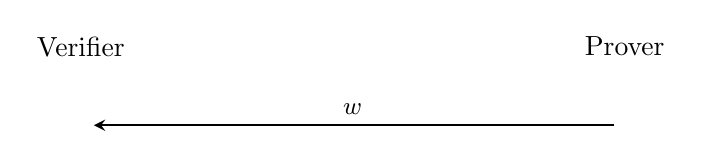
\begin{tikzpicture}[->,>=stealth,shorten >=1pt,auto,node distance=1cm,thick,main node/.style={scale=0.8,circle,draw,font=\sffamily\normalsize}]
            \node[] (1) []{$\mathrm{Verifier}$};
            \node[] (2) [left of = 1, xshift = 225]{$\mathrm{Prover}$};

            \node[] (3) [below of = 1]{};
            \node[] (4) [below of = 2]{};

            \path[every node/.style={font=\sffamily\small}]
                (4) edge[swap] node{$w$} (3)
                ;
        \end{tikzpicture}

        \caption{Message exchange for an $\mathsf{NP}$ language}
    \end{figure}
    
    However, we often need a more general way to convince the verifier of the validity of statements: we need to \textbf{interact} with it. In this model, the verifier asks a series of questions $q_1, \ldots, q_k$ that the prover answers with $a_1, \ldots, a_k$, until the verifier is convinced of the truthfulness of the statement.

    \begin{figure}[H]
        \centering

        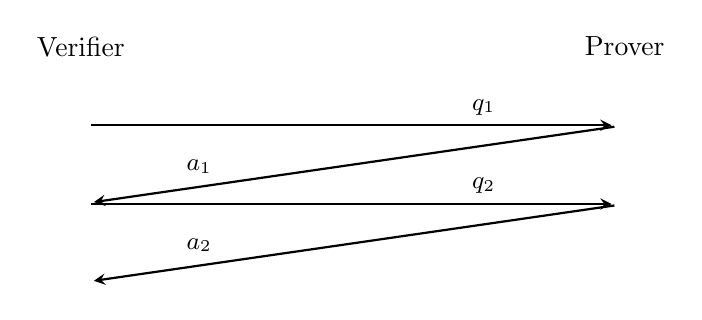
\begin{tikzpicture}[->,>=stealth,shorten >=1pt,auto,node distance=1cm,thick,main node/.style={scale=0.8,circle,draw,font=\sffamily\normalsize}]
            \node[] (1) []{$\mathrm{Verifier}$};
            \node[] (2) [left of = 1, xshift = 225]{$\mathrm{Prover}$};

            \node[] (3) [below of = 1]{};
            \node[] (4) [below of = 2]{};

            \node[] (5) [below of = 3]{};
            \node[] (6) [below of = 4]{};

            \node[] (7) [below of = 5]{};
            \node[] (8) [below of = 6]{};

            \path[every node/.style={font=\sffamily\small}]
                (3) edge[near end] node{$q_1$} (4)
                (4) edge[swap, near end] node{$a_1$} (5)
                (5) edge[near end] node{$q_2$} (6)
                (6) edge[swap, near end] node{$a_2$} (7)
                ;
        \end{tikzpicture}

        \caption{Message exchange in an $4$ round interactive proof}
    \end{figure}

    \newpage

    By this we mean that the verifier and prover are two variable-input deterministic functions $V,P$ that at each round of interaction compute the next question/answer as a function of the input and the interactions of the previous rounds.
    \[\begin{split}
        q_1 &= V(x) \\
        a_1 &= P(x,q_1) \\
        q_2 &= V(x,q_1,a_1) \\
        \vdots & \qquad \vdots \\
        q_{k} &= V(x,q_1,a_1, \ldots, q_{k-1}, a_{k-1}) \\
        a_{k} &= P(x,q_1,a_1, \ldots, q_{k-1}, a_{k-1}, q_k) \\
    \end{split}\]

    After the verifier receives the last answer from the prover, it outputs either a 0 or a 1. The output of $V$ at the end of the interaction denoted $\mathrm{out}_V\abk{V,P}(x)$ and it is defined to be $V(x,q_1,a_1, \ldots, q_{k}, a_{k})$. 

    We say that a language $L$ has a $k$-round \textbf{deterministic interactive proof system} if there's a deterministic \TM $V$ that can have a $k$-round interaction with any function $P: \{0,1\}^* \to \{0,1\}^*$ such that:
    \[x \in L \implies \exists P \;\; \mathrm{out}_V\abk{V,P}(x) = 1\]
    \[x \notin L \implies \forall P \;\; \mathrm{out}_V\abk{V,P}(x) = 0\]
    
    The class $\mathrm{dIP}$ contains all languages that have a polynomial time verifier and a $q(n)$-round deterministic interactive proof system where $q(n)$ is polynomial in $n$ -- in other words, $V$ runs in polynomial time and there are a polynomial amount of interactions. We notice that, by definition, the power of the prover has \underline{no limits}. This is intentional: the prover should be an omniscient being that can answer all questions. However, we notice that in order for $V$ to check the answers of $P$, they must have a polynomial size.

    This new class seems to be defined by a stronger model. In fact, it's easy to see that $\mathsf{NP} \subseteq \mathsf{dIP}$ since any $\mathsf{NP}$ proof is basically a one round deterministic proof. However, we can also show that $\mathsf{dIP} \subseteq \mathsf{NP}$ is also true. Since the verifier $V$ runs in polynomial time $p(n)$ and there are a polynomial $q(n)$ amount of rounds that generate the messages $q_1, a_1, \ldots, q_{\frac{q(x)}{2}-1}, a_{\frac{q(x)}{2}}$, we can define a new verifier $V'$ that takes all these messages as a single certificate and internally simulates both $V$ and $P$. Both the running time of $V'$ and the length of the new certificate are bounded by $p(n) q(n)$, concluding that $\mathsf{NP} = \mathsf{dIP}$.
    
    Where does the model fail? Shouldn't interaction allow us to achieve stronger proofs? Let's take a step back: we tried to model an interactive proof between two agents, but we assumed that the verifier will always yield the same answer on each step. In order to get a stronger model, we have to \textit{get rid of determinism}: we allow the verifier to use \textbf{randomness}. The idea behind this shift in prospective is simple: if we can convince the verifier with a high enough probability that the proof is valid even when he flips random coins, then the proof must be true.
    
    For example, suppose that you have a friend who is colorblind and that you aren't. You try to tell him that he can't distinguish between blue and red, but he doesn't believe you. How can you prove him that you're right? You ask him to take a red ball and a blue ball, one in the left hand and one in the right hand. Then, you ask him to hide them behind his back, randomly swap their positions, show the results and tell you if the one in the left hand is red or not. Since you're the all-mighty prover, you know if he's right or not. Hence, your answer has $\frac{1}{2}$ probability of being different from his answer (remember that you can distinguish the two colors, but he can't). After repeating this process enough times, the probability of you being always right will be way to high, meaning that your friend will have no choice but to accept the truth. Clearly, if we didn't allow randomness, this whole interaction would be useless, giving a good idea behind the strength of this new model.

    \begin{frameddefn}{The class $\mathsf{IP}$}
        We define $\mathsf{IP}$ as the class of languages for which there is a polynomial $\mathsf{PTM}$ $V$ that can have a $\mathrm{poly}(n)$-round interaction with any function $P: \{0,1\}^* \to \{0,1\}^*$:
        \[x \in L \implies \exists P \;\; \Pr[\mathrm{out}_V\abk{V,P}(x) = 1] \geq \frac{2}{3}\]
        \[x \notin L \implies \forall P \;\; \Pr[\mathrm{out}_V\abk{V,P}(x) = 1] \leq \frac{1}{3}\]

        If when $x \in L$ the probability of accepting is 1, we say that the interaction has \textbf{perfect completeness}.
    \end{frameddefn}

    As for the classes $\mathsf{BPP}, \mathsf{RP}$ and $\mathsf{coRP}$, we can boost the probability by running the verifier multiple times, hence the given definition is sufficient. 
    
    We discussed how the verifier \underline{must} use randomness. But doesn't the prover also have to use it? Wouldn't we obtain a stronger model? Suppose that the prover has to answer the question $q_i$ and that the can randomly produce one of three answers $\alpha^1_i, \alpha^2_i, \alpha^3_i$. Each of these answers gives us a different probability for the final acceptance of $V$ -- in other words, each answer produces a computational path that has a different probability of accepting. Notice that the probability given by one of these answers must be equal to at least the mean of the three probabilities. These probabilities can be inductively computed, starting from the leaves of the interaction tree and going up until the root is reached.Since the prover can be all-mighty, we can define a new deterministic prover that always produces the answer with the highest probability. In other words, due to there being no limits on the prover, a deterministic prover can simulate a probabilistic one.

    At this point, anyone would ask himself the following question: doesn't the unlimited power of the prover make the system too strong? The short answer would be yes, but only to some extent. In fact, in the definition that we gave the prover can be any function, even an uncomputable one. Let $V$ be the verifier for a language $L \in \mathsf{IP}$. By definition, any computation done by $V$ requires polynomial time and any interaction between $V$ and a prover requires a polynomial amount of computation. Hence, for any path in the interaction tree requires polynomial time to be computed. This means that polynomial space suffices to simulate a single path. By reusing this space, we can simulate any possible path of any possible prover. This concludes that $\mathsf{IP} \subseteq \mathsf{PSPACE}$.

    This result shouldn't come as a surprise: any interactive proof can be viewed as nothing more than a 2-player game with a bounded number of moves, which is easily reducible to $\mathsf{TQBF}$ as we discussed in the previous chapter. In later sections, we will show that of 2-player games and interactive proofs are indeed equivalent, i.e. that $\mathsf{IP} = \mathsf{PSPACE}$.

    Finally, we notice that we can also reduce the number of rounds needed by an interactive proof by \textit{parallelizing} it: instead of asking a single question, the verifier asks a bunch of questions and the prover provides a bunch of answers. These sets of questions and answers must be carefully selected to guarantee that the probabilities are left unchanged.

    \section{Public coins and the classes $\mathsf{AM}, \mathsf{MA}$}

    In the previous section, we defined the class $\mathsf{IP}$ through randomness. In that context, the random bits generated by the verifier are kept secret from the prover. This type of randomness is called \textbf{private coin} randomness. What happens if the prover can see the result of the verifier's flips, that is if the verifier uses \textbf{public coins}. Clearly, we expect this model to be stronger than the standard one. In fact, these types of interactive proofs are also called \textit{Arthur-Merlin proofs}. 
    
    According to an old legend, Arthur was a great king of medieval England and Merlin was his court magician. \textcite{arthur_merlin} used the name \curlyquotes{Arthur-Merlin} for this public coin model by drawing an analogy between the prover's
    infinite power and Merlin's magic. While Merlin cannot predict the coins that Arthur will toss in the future, Arthur has no way of hiding from Merlin's magic the results of the coins he tossed in the past.

    We notice that since Merlin can see the coins, there is no reason for Arthur to communicate his message since it will strictly depend from the results of the coins, which can already be seen by Merlin. For this reason, we can assume that Arthur communicates only the results of the coins -- basically, in this model Arthur yells random words and Merlin has to figure out a way to convince him. This means that any public coin proof can be seen as a private coin proof where the result of the coins is the communicated message.
    
    Moreover, we notice that in this context it is very important to distinguish who speaks first: if Arthur starts the conversation, Merlin has access to an additional information. When Merlin speaks first, we say that it is a \textit{Merlin-Arthur proof}.
    
    \begin{frameddefn}{The classes $\mathsf{AM}$ and $\mathsf{MA}$}
        For every value $k > 0$ (which can also not be a constant), we define $\mathsf{AM}[k]$ as the class of languages for which there is a $k$-round polynomial time Arthur-Merlin proof. Likewise, for every value $k > 0$, we define $\mathsf{MA}[k]$ as the class of languages for which there is a $k$-round polynomial time Merlin-Arthur proof. 
    \end{frameddefn}

    To clarify this notation, we observe that the classes $\mathsf{AM}[2]$ and $\mathsf{MA}[2]$ can be simply written as $\mathsf{AM}$ and $\mathsf{MA}$, while the class $\mathsf{AM}[5]$ can be written as $\mathsf{AMAMA}$.
    
    \begin{framedprop}[]{}
        For any constant $k > 1$ it holds that:
        \begin{enumerate}
            \item $\mathsf{A} = \mathsf{BPP}$
            \item $\mathsf{M} = \mathsf{NP}$
            \item $\mathsf{AM}[k] \subseteq \mathsf{IP}[k]$ 
            \item $\mathsf{AM}[k] \subseteq \mathsf{AM}[k+1]$
            \item $\mathsf{MA}[k] \subseteq \mathsf{MA}[k+1]$ 
            \item $\mathsf{MA}[k] \subseteq \mathsf{AM}[k+1]$
        \end{enumerate}
    \end{framedprop}

    \begin{proof}

        \quad

        \begin{enumerate}
            \item A single Arthur message is equivalent to a randomized string.
            \item A single Merlin message is equivalent to a witness.
            \item Any public coin proof can be simulated through a private coin proof where the verifier sends the generated random bits.
            \item Given a protocol $P$ for a language $L \in \mathsf{AM[k]}$, we can define a new protocol $P'$ with $k+1$ rounds and where Arthur speaks first. The first $k$ rounds are equivalent to those of $P$, while the last round is simply ignore since the first $k$ rounds are already enough to convince Arthur with a good probability.
            \item Equivalent to the proof of the previous proposition
            \item Given a protocol $P$ for a language $L \in \mathsf{MA[k]}$, we can define a new protocol $P'$ with $k+1$ rounds and where Arthur speaks first. The first round is simply ignored by Merlin, while the last $k$ rounds are equivalent to those of $P$ since they suffice to convince Arthur with a good probability.
        \end{enumerate}
    \end{proof}
    
    Here, the class $\mathsf{IP}[k]$ is the subset of $\mathsf{IP}$ languages that have a $k$-round proof. While it's easy to prove that private coin proofs are capable of simulating public coins, \textcite{gold_sipser} showed in a suprising result that the opposite also holds, with a small constant blow-up in the number of sent messages. We won't dive into this proof -- due to it being too long -- but we'll give the general idea: Arthur sends a random hash string that acts as the private bits and Merlin uses his all-mighty power to guess the encrypted message.

    \begin{framedthm}{The Goldwasser-Sipser theorem}
        For any constant $k > 1$, it holds that $\mathsf{IP}[k] \subseteq \mathsf{AM}[k+2]$
    \end{framedthm}
    
    \begin{proof} Omitted. \end{proof}
    
    An even more surprising result is given by the capability of Arthur-Merlin protocols to use less messages than it suffices. The idea is similar to what we discussed in parallelized interactive proofs: either Arthur sends a message that is equivalent to the next two questions, transforming a $\mathsf{AMA}$ interaction to a $\mathsf{AAM}$ interaction, or Merlin sends a message that is equivalent to the next two answers, transforming a $\mathsf{MAM}$ interaction to a $\mathsf{MMA}$ interaction. The result was proven by \textcite{babai_moran}.

    \begin{framedthm}{The Babai-Moran theorem}
        For any constant $k > 1$, it holds that $\mathsf{AM}[k+1] \subseteq \mathsf{AM}[k]$
    \end{framedthm}

    \begin{proof} Omitted. \end{proof}

    \begin{framedcor}{}
        $\mathsf{MA} \subseteq \mathsf{AM} = \mathsf{IP}[2]$
    \end{framedcor}

    \begin{proof}
        Follows from the two previous theorems and the previous proposition
    \end{proof}
    
    In particular, the collapse $\mathsf{AM} = \mathsf{AM}[k]$ for all constants $k > 0$ is somewhat surprising: $\mathsf{AM}[k]$ seems similar to $\Pi_k^P$, where the $\forall$ quantifiers are changed to a \curlyquotes{probabilistic} quantifier where most of the branches lead to acceptance. Hence, looks like this small difference is enough to make the $\mathsf{AM}[k]$ hierarchy collapse. However, the two classes are indeed related to the polynomial hierarchy.

    \begin{framedthm}{}
        $\mathsf{AM} \subseteq \Pi_2^p$ and $\mathsf{MA} \subseteq \Sigma_2^p \cap \Pi_2^p$
    \end{framedthm}

    \begin{proof}
        We'll start by proving that $\mathsf{AM} \subseteq \Pi_2^p$. Let $M$ be the machine for which $L \in \mathsf{AM}$. Consider the set $S_x = \{r \in \{0,1\}^m \mid \exists w \; M(x,r,w) = 1\}$. By applying the covering argument of \nameref{sips_gacs} on the set $\overline{S_x} = \{r \in \{0,1\}^m \mid \forall w  \in \{0,1\}^m \; M(x,r,w) = 0\}$, we get that:
        \[x \in \overline{L} \iff \exists \abk{u_1, \ldots, u_k} \in \{0,1\}^{O(mk)} \; \forall r \in \{0,1\}^m \;\; \bigvee_{i = 1}^k \forall w \; M(x, r \oplus u_i, w) = 0\]

        which is equivalent to:
        \[x \in L \iff \forall \abk{u_1, \ldots, u_k} \in \{0,1\}^{O(mk)} \; \exists r \in \{0,1\}^m \;\; \bigwedge_{i = 1}^k \exists w \in \{0,1\}^m \; M(x, r \oplus u_i, w) = 1\]

        We can now move the inner $\exists w$ statement to the outside one by quantifying on multiple strings. We get that $x \in L$ if and only if:
        \[\forall \abk{u_1, \ldots, u_k} \in \{0,1\}^{O(mk)} \; \exists \abk{r, w_1, \ldots, w_k} \in \{0,1\}^{O(mk)} \;\; \bigwedge_{i = 1}^k \; M(x, r \oplus u_i, w_i) = 1\]
        
        concluding that $L \in \Pi_2^P$. The whole argument can be summarized through a less formal one based only on quantifying operators. We define $\reflectbox{B}$ as the quantifying operator \curlyquotes{for most strings}, symbolizing the concept of randomness used in $\mathsf{BPP}$. Using the same notation as the polynomial hierarchy, we have that $\mathsf{AM} = \reflectbox{B} \exists P$. Then, since $\mathsf{BPP} \subseteq \Pi_2^P$, we conclude that:
        \[\mathsf{AM} = \reflectbox{B}\exists P \subseteq \forall \exists \exists P = \forall \exists P = \Pi_2^P\]

        Through the same idea (both the formal and informal one) using the fact that $\mathsf{MA} = \exists \reflectbox{B} P$ and $\mathsf{BPP} \subseteq \Sigma_2^P$, we get that:
        \[\mathsf{MA} = \exists \reflectbox{B} P \subseteq \exists \exists \forall P = \exists \forall P = \Sigma_2^P\]

        Finally, since we also know that $\mathsf{MA} \subseteq \mathsf{AM}$, we also get that $\mathsf{MA} \subseteq \Pi_2^P$.
    \end{proof}

    The above theorem shows that, Arthur-Merlin protocols with a constanst number of rounds are only slightly stronger than $\mathsf{NP}$. What about the class $\mathsf{coNP}$? Is it someway related to $\mathsf{AM}$ or $\mathsf{MA}$? \textcite{conp_int_proof} showed that if $\mathsf{coNP} \subseteq \mathsf{AM}$ -- and thus also if $\mathsf{coNP} \subseteq \mathsf{MA}$ since $\mathsf{MA} \subseteq \mathsf{AM}$ -- the whole polynomial hierarchy would collapse to the second level. This is due to how, differently from $\Pi_2^P$, in $\mathsf{AM}[k]$ the collapse of the hierarchy holds.

    \begin{framedthm}[label=conp_am_collapse]{}
        If $\mathsf{coNP} \subseteq \mathsf{AM}$ then $\Sigma_2^P = \Pi_2^P$.
    \end{framedthm}

    \begin{proof}
        Using the same quantifying notation of the previous theorem, since $\mathsf{coNP} = \forall P$ we have that:
        \[\Sigma_2^P = \exists \forall P \subseteq \exists \reflectbox{B} \exists P = \mathsf{MAM} \subseteq \mathsf{AMAM} = \mathsf{AM} \subseteq \Pi_2^P\]
        hence $\Sigma_2^P = \Pi_2^P$ by duality.
    \end{proof}

    In \Cref{g_iso}, we discussed how the \textit{graph isomorphism problem} is a good candidate for being an $\mathsf{NP}$-Intermediate language, but we haven't discussed the reason why this is true. Now, we're ready to justify this result. We recall that:
    \[\mathrm{GI} = \{\abk{G_1, G_2} \mid G_1, G_2 \text{ are two graphs s.t. } G_1 \cong G_2\}\]

    Two graphs $G_1, G_2$ are said to be isomorphic if they are the same up to a renumbering of the vertices; in other words, if there is a permutation $\pi$ of the labels of the nodes such that $\pi(G_1) = G_2$. Consider the opposite problem, that being the \textit{graph non-isomorphism problem}, defined as:
    \[\mathrm{GNI} = \{\abk{G_1, G_2} \mid G_1, G_2 \text{ are two graphs s.t. } G_1 \not\cong G_2\}\]

    \begin{framedprop}{}
        $\mathrm{GNI} \in \mathsf{AM}$
    \end{framedprop}

    \begin{proof}
        First, we show that $\mathrm{GNI} \in \mathsf{IP}[2]$ through the following interactive proof:
        \begin{enumerate}
            \item Given $\abk{G_1, G_2}$ in input, $V$ picks a random $i \in \{1,2\}$, randomly computes a permutation $\pi$ and sends $H = \pi(G_i)$ to $P$.
            \item Upon receiving $H$, $P$ figures out if $H$ is a permutation of $G_1$ or $G_2$. Let $j \in \{1,2\}$ be $P$'s answer. $P$ sends $j$ to $V$.
            \item If $i = j$, $V$ accepts
        \end{enumerate}

        We notice that if $G_1 \not\cong G_2$, then the prover will always be right. Hence, we have that $\Pr[\mathrm{out}_V\abk{V,P}(\abk{G_1,G_2}) = 1] = 1$, thus this interaction also has prefect completeness. If $G_1 \cong G_2$, instead, $P$ will have a $\frac{1}{2}$ chance of being wrong. By repeating the process enough times, we can boost the probability to the desired value. We conclude that $\mathrm{GNI} \in \mathsf{IP}[2] \subseteq \mathsf{AM}[4] = \mathsf{AM}$.
    \end{proof}

    It's obvious that $\overline{\mathrm{GI}} \leq_P \mathrm{GNI}$ and $\mathrm{GNI}\leq_P \overline{\mathrm{GI}}$, making the two problems equivalent. Thus, since $\mathrm{GI} \in \mathsf{NP}$, we have that $\mathrm{GNI} \in \mathsf{coNP}$ also holds. If $\mathrm{GI}$ where to be $\mathsf{NP}$-Complete then $\mathrm{GNI}$ would be $\mathsf{coNP}$-Complete. Hence, since $\mathrm{GNI} \in \mathsf{coNP} \cap \mathsf{AM}$, we would get that $\mathsf{coNP} \subseteq \mathsf{AM}$, making the polynomial hierarchy collapse by \Cref{conp_am_collapse}.
    
    \begin{framedcor}{}
        If $\mathrm{GI}$ is $\mathsf{NP}$-Complete then $\Sigma_2^P = \Pi_2^P$
    \end{framedcor}

    \section{The power of interaction}

    Until 1990, all we knew was that $\mathsf{NP} \subseteq \mathsf{IP} \subseteq \mathsf{PSPACE}$ and there was evidence that the first containment would be proper. Most researchers felt that the second containment would also be proper. We know that interaction alone does not give us any languages outside $\mathsf{NP}$ -- remember that $\mathsf{dIP} = \mathsf{NP}$ -- and we also suspect that randomization alone shouldn't add significant power to computation -- remember that we suspect that $\mathsf{BPP} = \mathsf{P}$. So how much more power could the combination of randomization and interaction provide? Researchers believed that the answer would be \curlyquotes{not much power} due to the following facts:
    \begin{enumerate}
        \item There were no protocols known that required $k$ to not be a constant, so $\mathsf{IP} = \mathsf{IP}[\mathrm{poly}(n)]$ did not seem much bigger than $\mathsf{IP}[O(1)]$
        \item For any constant $k > 0$, $\mathsf{IP}[k]$ collapses to the class $\mathsf{AM}$, which seems to be only slightly more powerful than $\mathsf{NP}$ (since we're just flipping some coins before sending the certificate)
        \item The inclusion $\mathsf{coNP} \subseteq \mathsf{AM}$ probably doesn't hold since otherwise the polynomial hierarchy collapses, making $\mathsf{coNP} \subseteq \mathsf{AM}$ unlikely to be true
    \end{enumerate}

    In a ground-breaking result, \textcite{shamir} -- on of the three creators of RSA -- proved that $\mathsf{PSPACE} \subseteq \mathsf{IP}$, giving a surprising characterization of $\mathsf{IP}$ and showing that these intuitions were drastically wrong. Many researchers explored the techniques used by Shamir to achieve his result, in particular his \textbf{arithmetization} technique. Let $\phi = \bigwedge_{i = 1}^m C_i$ be a CNF formula. For each clause $C_i$, we want to define a polynomial $P_C$ such that $C_i(\alpha) = 1$ if and only if $P_{C_i}(\alpha) = 1$. This polynomial is inductively constructed as follows:
    \begin{itemize}
        \item A variable $x_i$ is mapped to $x_i$
        \item A negation $\overline{B}$ where $B$ is a sub-formula is mapped to $1-P_B$
        \item A conjunction $A \land B$ is mapped to $P_A \cdot P_B$
        \item A disjunction $A \lor B$ is mapped to $1- (1-P_A)(1-P_B)$
    \end{itemize}

    We notice that the last encoding comes from the fact that $A \lor B = \overline{\overline{A} \land \overline{B}}$. For example, given the clause $x_1 \lor \overline{x_2} \lor x_3$, we define the polynomial $P_{C_i}(x) = 1 - (1-x_1) x_2 (1-x_3)$. For a whole formula $\phi$, we denote the corresponding polynomial with $P_\phi$. We notice that  $P_\phi(\alpha)$ always evaluates to either to 0 or 1.
    
    To give an intuition behind how this concept can be used in interactive proofs, we first prove a less powerful statement that proves wrong the third intuition listed above.

    \begin{framedthm}{}
        $\mathsf{coNP} \subseteq \mathsf{IP}$
    \end{framedthm}

    \begin{proof}
        Let $\mathrm{\#SAT}$ -- pronounced \textit{sharp SAT} -- be the search problem that asks to find the number of satisfying assignments for a CNF formula $\phi$. The decisional version of this problem is defined as:
        \[\mathrm{\#SAT_D} = \{\abk{\phi, k} \mid \phi \text{ is a CNF with exactly $k$ satisfying assignments}\}\]

        It's easy to see that $\mathrm{UNSAT} \leq_P \mathrm{\#SAT_D}$ since the former is a special case of the latter (when $k = 0$). This means that $\mathrm{\#SAT_D}$ is $\mathsf{coNP}$-Hard. Hence, in order to prove that $\mathsf{coNP} \subseteq \mathsf{IP}$ it is sufficient to show that $\mathrm{\#SAT_D} \in \mathsf{IP}$.

        Let $\phi$ be a CNF formula and let $P_\phi$ be the polynomial given by its arithmetization. Since $\phi$ is a CNF formula, we have that $P_\phi = \prod_{i = 1}^{m} P_{C_i}$. In particular, this also implies that $\mathrm{deg}(P_\phi)$ is at most equal to the total number of literals inside every clause of $\phi$. Let $\#\phi$ be the number of satisfying assignments of $\phi$. We notice that:
        \[\#\phi = \sum_{b_1 \in \{0,1\}} \sum_{b_2 \in \{0,1\}} \ldots \sum_{b_n \in \{0,1\}} P_{\phi}(b_1, \ldots, b_n)\]

        However, we cannot simply compute this sum since the numbers inside it may get too big, requiring exponential time to compute. To fix this issue, we notice that $0 \leq \#\phi \leq 2^n$, since at most all the assignments can satisfy $\phi$. Hence, if we pick a prime $p$ such that $2^n < p \leq 2^{2n}$, which is always guaranteed to exist, we get that:
        \[\#\phi = \sum_{b \in \{0,1\}^n} P_{\phi}(b_1, \ldots, b_n) \iff \#\phi \equiv \sum_{b \in \{0,1\}^n} P_{\phi}(b_1, \ldots, b_n) \pmod{p}\]

        Since $p \leq 2^{2n}$, we require at most $2n$ bits to compute a number in $\F_p$. To ensure that the picked value is a prime number, we can use the randomized algorithm showed in \Cref{random_power}. From now on all the computations will be assumed to be made in $\F_p$. Given a degree $d$ polynomial $g(y_1, \ldots, y_t)$, an integer $z \geq 0$ and a prime $q$, we provide a general \textit{sum-check protocol} that enables us to verify that:
        \[z \equiv \sum_{b \in \{0,1\}^n} g(b_1, \ldots, b_n) \pmod{q}\]

        \texttt{Sum-check-protocol:}
        \begin{enumerate}
            \item Given $\abk{g,z,q}$ in input, if $n = 1$ then $V$ checks if $g(0) + g(1) \equiv z \pmod{q}$, accepting if it's true and rejecting otherwise.
            \item If $n > 1$, $V$ asks $P$ to send a polynomial.
            \item $P$ sends a polynomial $s(x)$
            \item $V$ checks if $s(0) + s(1) \not\equiv z \pmod{q}$. If true, $V$ rejects. Otherwise, $V$ picks a random $a \in \F_q$ and recursively runs the sum-check protocol to verify that $s(a) \equiv \sum\limits_{b \in \{0,1\}^{n-1}} g(b_1, \ldots, b_{n-1}, a) \pmod{q}$
            \item If the recursive call accepts, $V$ accepts. Otherwise, $V$ rejects.
        \end{enumerate}
        
        When the verifier asks the prover to send the polynomial $s(x)$, the verifier expects an answer of the form:
        \[h(x) = \sum\limits_{b \in \{0,1\}^{n-1}} g(b_1, \ldots, b_{n-1}, x)\]

        We notice that when the input $\abk{g,z,q}$ is valid, i.e. when $z \equiv \sum_{b \in \{0,1\}^n} g(b_1, \ldots, b_n) \pmod{q}$ holds, it will always hold that $h(0) + h(1) = z$ is true. Hence, when the input is valid, if polynomial sent by the prover on each recursive call is always what the verifier expects then $V$ will accept with probability 1, meaning that this protocol has perfect completeness.

        When the prover is cheating, instead, $V$ will receive a polynomial $s(x)$ that is different from $h(x)$ but for which $s(0) + s(1) \equiv z \pmod(q)$ still holds. If the random value $a \in \F_q$ picked by the verifier satisfies the equation $s(a) \equiv h(a) \pmod{q}$ -- recall that $h(a) = \sum\limits_{b \in \{0,1\}^{n-1}} g(b_1, \ldots, b_{n-1}, a)$ -- the prover will have correctly fooled the verifier since the prover can proceed by sending the expected polynomial for the sequent recursions. We claim that the probability of this happening is very low.

        \textbf{Claim}: $\Pr[V(\abk{z,g,q}) = 0] \geq \rbk{1-\frac{d}{q}}^n$ when the equation $z \not\equiv \sum_{b \in \{0,1\}^n} g(b_1, \ldots, b_n) \pmod{q}$, where $d$ is the degree of $g$.

        \begin{proof}[Proof of the claim.]
            To make notation simpler, we assume that every computation in the proof of this claim is made in $\F_q$. Assume that the equation is false. We proceed by induction on $n$. When $n = 1$, $V$ evaluates $g(0) + g(1) = z$ and rejects with probability 1 if it isn'n true. Assume that the claim is true for any degree $d$ polynomial with $n-1$ variables.

            If the polynomial $s(x)$ returned by the prover is equal to $h(x)$ then the check $s(0) + s(1) \neq z$ will return true, making $V$ reject with probability 1. Suppose now that the prover sends a polynomial $s(x)$ different from $h(x)$ for which $s(0) + s(1) = z$ holds. Since the polynomial $s(x) - h(x) = 0$ has at most $d$ roots, there are at most $d$ values $a$ such that $s(a) = h(a)$. Hence, given a random $a \in \F_q$, we have that $\Pr[s(a) \neq h(a)] \geq 1 - \frac{d}{q}$

            When $s(a) \neq h(a)$ holds, by inductive hypothesis the probability, that the verifier rejects the input $\abk{s(a), h(a), q}$ is at least $\rbk{1-\frac{d}{q}}^{n-1}$. Thus, we get that:
            \[\Pr[V(\abk{z,g,q}) = 0 \text{ when the eq. is false}] =\]
            \[\Pr[s(a) \neq h(a) \;\land\; V(\abk{s(a),h(a),q}) = 0 \text{ when the eq. is false}]\]
            \[\geq \rbk{1 - \frac{d}{q}}\rbk{1 - \frac{d}{q}}^{n-1} = \rbk{1 - \frac{d}{q}}^n\]
        \end{proof}

        The claim concludes that the sum-check protocol is a valid polynomial interactive proof. Moreover, when we run the sum-check protocol with input $\abk{P_\phi, k, p}$, the protocol will accept with probability 1 if $k = \#\phi$ and reject with probability at least $\rbk{1 - \frac{\mathrm{deg}(\mathrm{P_\phi})}{p}}^n$, concluding that $\mathrm{\#SAT}$ is in $\mathsf{IP}$.
    \end{proof}

    Now that we understand how arithmetization can be used in the sum-checking protocol, we're ready to prove Shamir's result

    \begin{framedthm}{}
        $\mathsf{IP} = \mathsf{PSPACE}$
    \end{framedthm}

    \begin{proof}
        We already know that $\mathsf{IP} \subseteq \mathsf{PSPACE}$ and that $\mathrm{TQBF}$ is $\mathsf{PSPACE}$-Complete. Hence, it suffices to show a polynomial interactive protocol for $\mathrm{TQBF}$.

        Given a TQBF formula $\psi = Q_1 x_1 \; \ldots Q_n x_n \; \phi$, the arithmetization $P_\psi$ of $\psi$ is obtained by converting every $\forall$ quantifier into a $\Pi$ operator, while every $\exists$ quantifier is converted into a $\Sigma$ operator. For example, given $\psi = \forall x_1 \; \exists x_2 \; \exists x_3 \; \phi$, we have that:
        \[\#\psi = \prod_{b_1 \in \{0,1\}} \sum_{b_2 \in \{0,1\}} \sum_{b_3 \in \{0,1\}} P_\phi\]

        Since a QBF can only be true or false, the number of satisfying assignments has to be either 0 or 1. Hence, $\psi$ is true if and only if $\#\psi \neq 0$. We observe that could use the same sum-check protocol that we used for $\mathrm{\#SAT_D}$, with a little change: when the variable $x_i$ is quantified with $\forall$, we check that $s(0) \cdot s(1) = k$. There is nothing wrong with this procedure, except that the running time would become exponential: multiplying polynomials, unlike addition, increases the degree.

        This means that we have to use a different approach (meaning that we ignore the previous construction). We observe that since $b_1, \ldots, b_n \in \{0, 1\}$, we have that $b_i^k = b_i$ for all $k \geq 1$. Thus, we can convert any polynomial $P(y_1, \ldots , y_n)$ into a \textit{multilinear polynomial} $Q(y_1, \ldots , y_n)$, meaning that the degree of $Q(\cdot)$ in any variable $y_i$ is at most 1, that agrees with $P(\cdot)$ on all $y_1, \ldots, y_n \in \{0, 1\}$.
        
        We define a \textit{linearization} operator on polynomials where for any polynomial $P(\cdot)$ we denote with $L_{y_i}$ the polynomial linearized on $y_i$, defined as:
        \[L_{y_i}(P) = y_i \cdot P(y_1, \ldots,  y_{i-1}, 1, y_{i+1}, \ldots, y_n) + (1-y_i) P(y_1, \ldots,  y_{i-1}, 0, y_{i+1}, \ldots, y_n)\]

        Since $L_{y_i}(P)$ is linear in $y_i$ and agrees with $P(\cdot)$ whenever $y_i \in \{0, 1\}$, by applying this operator on all the variables we get that $L_{y_1}(L_{y_2}( \cdots (L_{y_n}(P)) \cdots))$ is a multilinear polynomial agreeing with $P(\cdot)$ on all values in $\{0, 1\}$. The mappings from $\forall$ to $\Pi$ and from $\exists$ to $\Sigma$, can also be defined al operators on polynomials, where:
        \[\forall_{y_i} P(y_1, \ldots, y_n) = P(y_1, \ldots,  y_{i-1}, 1, y_{i+1}, \ldots, y_n) \cdot P(y_1, \ldots,  y_{i-1}, 0, y_{i+1}, \ldots, y_n)\]
        \[\exists_{y_i} P(y_1, \ldots, y_n) = P(y_1, \ldots,  y_{i-1}, 1, y_{i+1}, \ldots, y_n) + P(y_1, \ldots,  y_{i-1}, 0, y_{i+1}, \ldots, y_n)\]

        We now get that if we apply the sequence of operators $Q_{y_1} \; \ldots \; Q_{y_n}$ (where $Q$ is either $\forall$ or $\exists$, $Q_{y_n}$ is applied first and $Q_{y_1}$ is applied last) on the polynomial $P_\phi(y_1, \ldots , y_n)$, we get a nonzero value $\#\psi$ if and only if $\psi$ is true. Since this claim only concerns values taken when variables are in $\{0, 1\}$, applying the linearization operator inside it won't change the correctness of the claim. We will \curlyquotes{sprinkle} in linearization operators so that the intermediate polynomials arising in our sum-check protocol all have low degree. In particular, we apply this operator in the following fashion:
        \[Q_{y_1} L_{y_1} \; Q_{y_2} L_{y_1} L_{y_2} \; \ldots \; Q_{y_n} L_{y_1} L_{y_{2}} \ldots L_{y_n} \; P_\phi(y_1, \ldots, y_n)\]

        This new expression has length $O(1 + 2 + \ldots + n) = O(n^2)$. We now have to define a variant of the sum-check protocol. We give an inductive description of this new protocol. Suppose for some polynomial $g(y_1 , \ldots , y_k)$ the prover has the ability to convince the verifier that $g(a_1 , a_2 , \ldots , a_k) = C$ with probability 1 for any $a_1 , a_2 , . . . , a_k, C$ when the equation is true and  with probability less than $\varepsilon$ when it is false. Let $U(y_1 , y_2 , \ldots , y_\ell )$ be any polynomial on $\ell$ variables such that $U(y_1 , \ldots , X_\ell ) = O \; g(y_1 , \ldots , y_k)$ where $O$ is an operator chosen from $\forall_{y_i}, \exists_{y_i}$ and $L_{y_i}$ (hence $\ell$ is $k-1$ in the first two cases and $k$ in the third case). Let $d$ be an upper bound known to the verifier of the degree of $x_i$ inside $U$. By construction of $P_\phi$ we know that $d$ is at most $3m$.

        We show how the prover can convince the verifier that $U(a_1 , a_2 , \ldots , a_\ell ) = C'$ with probability 1 for any $a_1 , a_2 , \ldots , a_k, C'$ for which it is true and with probability at most $\varepsilon + \frac{d}{p}$ when it is false where $p$ is derived in the same way as the previous proof. By renaming variables if necessary, assume $i = 1$. We have three cases:
        \begin{itemize}
            \item If $O = \exists_{y_1}$ then the prover provides a degree $d$ polynomial $s(y_1)$ -- which is supposed to be equal to $g(y_1, a_1, \ldots, a_k)$ when the prover is not cheating. The verifier checks if $s(0) + s(1) = C'$. If the check fails, the verifier rejects. Otherwise, the verifier picks a random value $a \in \F_p$ and recursively asks the prover to prove that $s(a) = g(a, a_2, \ldots, a_k)$
            \item If $O = \forall_{y_1}$ then we procede as the previous case, but we check that $s(0) \cdot s(1) = C'$ instead of $s(0) + s(1) = C'$
            \item If $O = L_{y_1}$ then the prover wishes to convince the verifier that $U(a_1 , a_2 , \ldots , a_k ) = C'$. The prover provides a degree $d$ polynomial $s(y_1)$ -- which is supposed to be equal to $g(y_1, a_1, \ldots, a_k)$ when the prover is not cheating. The verifier checks that $a_1 \cdot s(0) + (1-a_1) \cdot s(1) = C'$. If the check fails, the verifier rejects. Otherwise, the verifier picks a random value $a \in \F_p$ and recursively asks the prover to prove that $s(a) = g(a, a_2, \ldots, a_k)$
        \end{itemize}

        The proof of correctness of this protocol follows in the same way that we proved the correctness of the previous sum-check protocol, concluding that $\mathrm{TQBF} \in \mathsf{IP}$
    \end{proof}

    \begin{figure}[H]
        \centering

        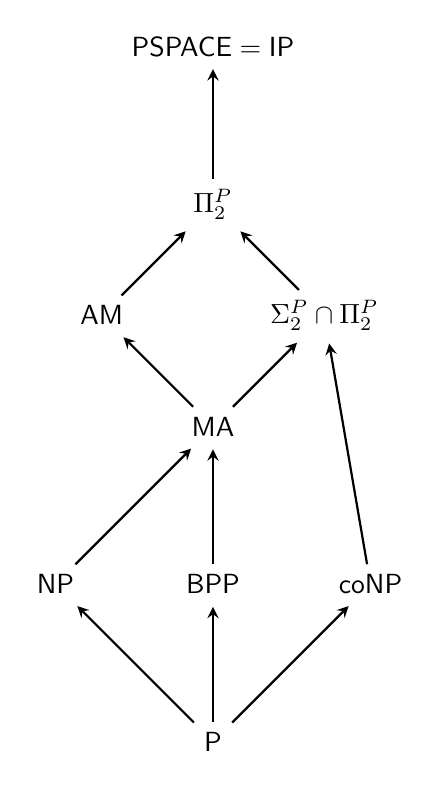
\begin{tikzpicture}[->,>=stealth,shorten >=1pt,auto,node distance=2cm,thick,main node/.style={scale=0.8,circle,draw,font=\sffamily\normalsize}]
            \node[] (1) []{$\mathsf{P}$};

            \node[] (2) [above of = 1]{$\mathsf{BPP}$};
            \node[] (3) [left of = 2]{$\mathsf{NP}$};
            \node[] (4) [right of = 2]{$\mathsf{coNP}$};

            \node[] (5) [above of = 2]{$\mathsf{MA}$};
            \node[] (6) [above left of = 5]{$\mathsf{AM}$};
            \node[] (7) [above right of = 5]{$\Sigma_2^P \cap \Pi_2^P$};

            \node[] (8) [above left of = 7]{$\Pi_2^P$};
            \node[] (9) [above of = 8]{$\mathsf{PSPACE} = \mathsf{IP}$};
            
            \path[every node/.style={font=\sffamily\small}]
                (1) edge (2)
                (1) edge (3)
                (1) edge (4)
                (2) edge (5)
                (3) edge (5)
                (4) edge (7)
                (5) edge (6)
                (5) edge (7)
                (6) edge (8)
                (7) edge (8)
                (8) edge (9)
                ;
        \end{tikzpicture}

        \caption{Summary of the class inclusions discussed in this chapter}
    \end{figure}


    \chapter{Query complexity}

    \section{Decision trees}

    Until now, we have focused on general complexity, discussing how many resources are needed by a Turing machine to solve or verify a problem. Now, we'll focus on the \textbf{concrete complexity} of problems, i.e. how hard the problem is by its own nature, using \curlyquotes{graph-like} abstract computational models. First, we'll focus on \textit{decision trees}. 

    \begin{frameddefn}{Decision tree}
     A \textbf{decision tree} is a rooted directed binary tree whose nodes are associated with either an input Boolean variable or an output value chosen between 0 or 1. Each internal node is labeled by a variable and the two outgoing edges are labeled by the two possible values of that variable.
    \end{frameddefn}

    Given an input $x \in \{0,1\}^n$, the computation made by a decision tree proceedes as follows. Initially, the input $x$ is unknown by the tree. Starting from the root, the decision tree makes a \textbf{query} asking the value of the bit $x_i$ that labels the current node. The query gets answered by an all-mighty user -- which can be imagined as an oracle-like machine or a human being -- that knows every bit of the input string $x$, answering with the value of $x_i$ for the given input $x$. 
    
    Based on the answer of the query, the computation proceeds on the edge corresponding to the answer, using the fact that the value of $x_i$ is known by the decision tree. When a leaf node is reached, the decision tree outputs the value that labels such leaf.

    The labels of the nodes don't have to be in any specific order. For instance, in a path we may first query the bit $x_5$ and then the bit $x_1$. 

    \begin{figure}[H]
        \centering

        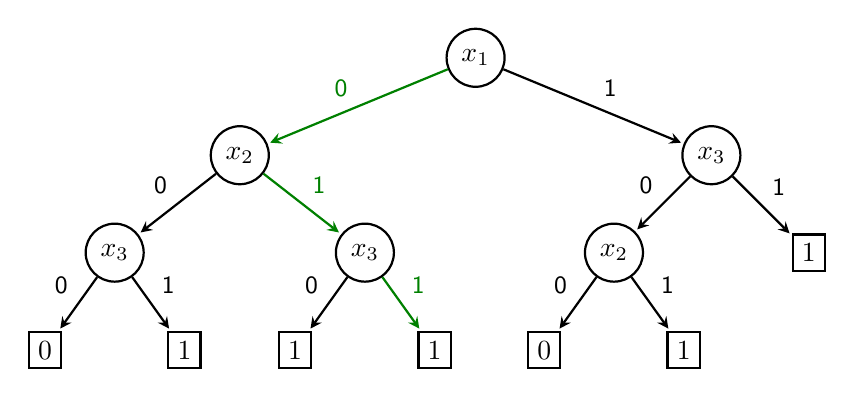
\begin{tikzpicture}[->,>=stealth,shorten >=1pt,auto,node distance=1.75cm, thick,main node/.style={scale=0.9,circle,draw,font=\sffamily\normalsize}]

            \node[circle, draw] (1)[] {$x_1$};

            \node[circle, draw] (2) [below left of=1, xshift=-50, ]{$x_2$};
            \node[circle, draw] (3) [below right of=1, xshift=50, ]{$x_3$};

            \node[circle, draw] (4) [below left of=2, xshift=-10, ]{$x_3$};
            \node[circle, draw] (5) [below right of=2, xshift=10, ]{$x_3$};
            \node[circle, draw] (6) [below left of=3, ]{$x_2$};
            \node[rectangle, draw] (7) [below right of=3]{$1$};

            \node[rectangle, draw] (8) [below left of=4, xshift=10]{$0$};
            \node[rectangle, draw] (9) [below right of=4, xshift=-10]{$1$};
            \node[rectangle, draw] (10) [below left of=5, xshift=10]{$1$};
            \node[rectangle, draw] (11) [below right of=5, xshift=-10]{$1$};
            \node[rectangle, draw] (12) [below left of=6, xshift=10]{$0$};
            \node[rectangle, draw] (13) [below right of=6, xshift=-10]{$1$};

            \path[every node/.style={font=\sffamily\small}]
                (1) edge[swap, color=Green]  node{0} (2)
                (1) edge node{1}(3)

                (2) edge[swap]  node{0} (4)
                (2) edge[color=Green]  node{1}(5)

                (3) edge[swap]  node{0} (6)
                (3) edge  node{1}(7)
                            
                (4) edge[swap]  node{0} (8)
                (4) edge  node{1}(9)

                (5) edge[swap]  node{0} (10)
                (5) edge[color=Green]  node{1}(11)

                (6) edge[swap]  node{0} (12)
                (6) edge  node{1}(13)
                ;
        \end{tikzpicture}

        \caption{An example of a decision tree. The green path shows the computation achieved through the input $x = 01101$}
    \end{figure}
    
    As for Boolean circuits, given a function $f : \{0,1\}^n \to \{0,1\}$ we say that a decision tree $T$ computes $f$ if for all inputs $x \in \{0,1\}^n$ it holds that $T(x) = f(x)$. Given a decision tree $T$, its \textit{size} is the number of nodes in the tree, while its \textit{depth} is the length of the longest path from the root to a leaf.

    \begin{figure}[H]
        \centering

        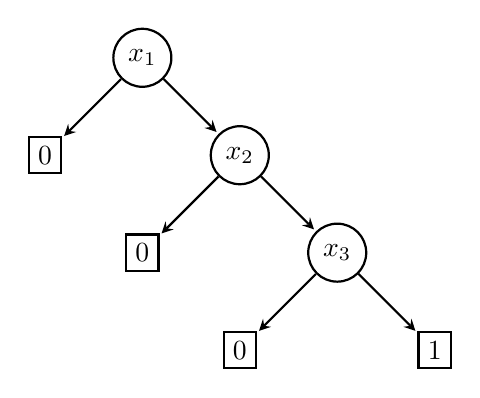
\begin{tikzpicture}[->,>=stealth,shorten >=1pt,auto,node distance=1.75cm, thick,main node/.style={scale=0.9,circle,draw,font=\sffamily\normalsize}]

            \node[circle, draw] (1)[] {$x_1$};

            \node[rectangle, draw] (2) [below left of=1]{$0$};
            \node[circle, draw] (3) [below right of=1]{$x_2$};

            \node[rectangle, draw] (4) [below left of=3]{$0$};
            \node[circle, draw] (5) [below right of=3]{$x_3$};

            \node[rectangle, draw] (6) [below left of=5]{$0$};
            \node[rectangle, draw] (7) [below right of=5]{$1$};

            \path[every node/.style={font=\sffamily\small}]
                (1) edge (2)
                (1) edge (3)
                (3) edge (4)
                (3) edge (5)
                (5) edge (6)
                (5) edge (7)
                ;
        \end{tikzpicture}

        \caption{A size 7, depth 3 decision tree computing $\mathrm{AND}(x_1, x_2, x_3)$}
    \end{figure}

    Differently from Boolean circuits, we're more interested in the depth of the tree instead of its size. This shift in prospective comes from the difference in how the computation works: Boolean circuits immediately compute the outpute, while decision trees have to query bits. Hence, we want to minimize the number of queries needed for a computation.
    
    Given an input $x$ and a decision tree $T$, the \textit{cost} of the computation $T(x)$, written as $\mathrm{cost}(T,x)$, is the length of the path in $T$ traversed by $x$. Let $\mathcal{T}_f$ be the set of all decision trees computing $f$. The \textbf{query complexity} of a function $f$, denoted as $D(f)$, is defined as the minimum depth of any decision tree in $\mathcal{T}_f$.
    \[D(f) = \min_{T \in \mathcal{T}_f} \max_{x \in \{0,1\}^n} \mathrm{cost}(T,x)\]
    
    We notice that, by definition, for every Boolean function $f : \{0,1\}^n \to \{0,1\}$ it must hold that $D(f) \leq n$ since we can query at most every input bit.
    
    \newpage

    In particular, in this scenario a computation is said to be \curlyquotes{efficient} if it requires a \textbf{poly-logarithmic number of queries} with respect to the input size.
    
    \begin{frameddefn}{$\mathsf{P}^{dt}$}
        We define $\mathsf{P}^{dt} = \{f : \{0,1\}^n \to \{0,1\} \mid D(f) \leq \log^k n\}$ as the query complexity analog of the class $\mathsf{P}$.
    \end{frameddefn}

    We observe that this class doesn't really have any connection to the class $\mathsf{P}$ since decision trees and Turing machines are \textit{incomparable}. Hence, it just acts as a notation that conveys the concept of efficient computation in query complexity.

    \section{Lower bounds for decision trees}

    Surprisingly, lots of elementary functions are very hard for decision trees. In particular, they strictly require decision trees of depth $n$ to be computed. To prove these lower bounds the common approach is to use an \textit{adversarial (or delayer) argument}.

    \begin{frameddefn}{Adversarial argument}
        Given a Boolean function $f : \{0,1\}^n \to \{0,1\}$, the \textbf{adversarial (or delayer) argument} proceedes as follows. By way of contradiction, we assume that there is a decision tree with depth at most $d$ that computes $f$ and impersonate an entity -- the delayer -- that answers the queries made by this tree with carefully chosen values, while keeping the answer ambiguous (hence delaying the final answer as much as possible), showing that the decision tree would need at least $d+1$ queries to give the final answer, raising a contradiction.
    \end{frameddefn}

    To show how this work, we'll prove that $D(\mathrm{AND}) \geq n$. Suppose that we a decision tree $T$ with depth $n-1$ that computes $\mathrm{AND}$ on $n$ bits. The delayer -- that being us -- impersonates the all-mighty user that answers $T$'s queries. W.l.o.g. we assume that the variables queried by this decision tree follow the order $x_1, \ldots, x_{n-1}$. For each $n-1$ variable, we answer the query with 1, meaning that $x_1, \ldots, x_{n-1} = 1$. By construction of the $\mathrm{AND}$ function, this isn't enough to decide the output: if $x_n = 0$ then the output will be 0, while if $x_n = 1$ then the output will be one. This implies that the tree must also query the last bit, concluding that $D(\mathrm{AND}) \geq n$. In a similar fashion, we can prove that $D(\mathrm{OR}) = D(\mathrm{PARITY}) = n$ by answering the first $n-1$ queries with 0: in both cases, the last bit will decide if the output is 0 or 1.


    Proving lower bounds with decision trees may seem useless. For instance, the $\mathrm{AND}$ function is hard for decision trees but is really easy for Turing machines. However, if we think of more complex problems, decision trees lower bounds, which highly depend on \textbf{combinatorial arguments}, are a good way to prove lower bounds even for Turing machines. 
    
    \newpage

    A common example of this is the \textbf{lower bound for comparison based sorting algorithms}. We know that $n$ values can be sorted in $n!$ ways by permuting the initial order. Using a generalized version of decision trees where the output is not restricted to a simple 0 or 1, meaning that we have a finite set of output values, the lowest possible depth of a decision tree with $n!$ leaves is $\Omega(\log n!)$ which is in the order of $\Omega(n \log n)$. Since a decision tree's queries are answered in time $O(1)$ by an omniscient being that requires, a Turing machine will also require at least time $\Omega(n \log n)$ even by simulating this decision tree (we can easily compute if $x_i < x_j$ in $O(1)$).

    To give another example, we'll show a lower bound for the \textit{graph connectivity function} $\mathrm{CONN}$ which, given an input graph $G$, returns 1 if the graph is connected and 0 otherwise. First, we need to model the input size accordingly: assuming that $G$'s vertices are represented by the set $\{1,\ldots, m\}$, $G$ will have at most $\binom{m}{2}$ edges -- which can be directed or not. The graph can be represented through its edges, meaning that we can assume that $\mathrm{CONN} : \{0,1\}^{\binom{m}{2}} : \{0,1\}$, where for each variable $x_{i,j}$ it holds that $x_{i,j} = 1$ if and only if $(i,j) \in E(G)$.

    We know that $D(\mathrm{CONN}) \leq \binom{m}{2}$. We'll prove that $D(\mathrm{CONN}) \geq \binom{m}{2}$ also holds. Again, we give an adversary argument. The adversary constructs a \curlyquotes{mental image} graph, edge by edge, as it responds to the decision tree's queries. The idea is that the delayer will use this mental image graph to trace what the prover knows about the \curlyquotes{fooling} input graph that gives a lower bound. Basically, we're constructing a counterexample query-by-query. After each step, the prover will only know only a part of this counterexample, which can always be extended to both a connected and disconnected graph using the edges that have not been queried so far, preserving the ambiguity of the answer.

    For every query $x_{i,j}$ made by the tree, we will answer 0 if by removing it from the mental image the latter may still be connected. Otherwise, if such an answer forces it to become disconnected -- which would allow the prover to give a definitive answer -- we answer with 1, making the answer still ambiguous. This strategy ensures that the partial graph known by prover after each query is always a \textit{forest}, i.e. it consists of vertex-disjoint trees, that turns into a whole connected graph only after the very last edge is queried. This concludes that $D(\mathrm{CONN}) = \binom{m}{2}$.

    \begin{figure}[H]
        \centering

        \begin{tabular}{ccccccc}
            \begin{tabular}{c}
                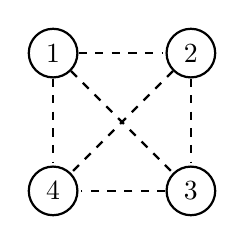
\begin{tikzpicture}[-,>=stealth,shorten >=1pt,auto,node distance=1.75cm, thick,main node/.style={scale=0.9,circle,draw,font=\sffamily\normalsize}]

                    \node[circle, draw] (1)[] {$1$};
                    \node[circle, draw] (2) [right of=1]{$2$};
                    \node[circle, draw] (3) [below of=2]{$3$};
                    \node[circle, draw] (4) [left of=3]{$4$};

                    \path[every node/.style={font=\sffamily\small}]
                        (1) edge[dashed] (2)
                        (1) edge[dashed] (3)
                        (1) edge[dashed] (4)
                        (2) edge[dashed] (3)
                        (2) edge[dashed] (4)
                        (3) edge[dashed] (4)
                        ;
                \end{tikzpicture}
            \end{tabular}

            &\quad&


            \begin{tabular}{c}
                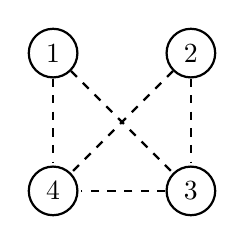
\begin{tikzpicture}[-,>=stealth,shorten >=1pt,auto,node distance=1.75cm, thick,main node/.style={scale=0.9,circle,draw,font=\sffamily\normalsize}]

                    \node[circle, draw] (1)[] {$1$};
                    \node[circle, draw] (2) [right of=1]{$2$};
                    \node[circle, draw] (3) [below of=2]{$3$};
                    \node[circle, draw] (4) [left of=3]{$4$};

                    \path[every node/.style={font=\sffamily\small}]
                        (1) edge[dashed] (3)
                        (1) edge[dashed] (4)
                        (2) edge[dashed] (3)
                        (2) edge[dashed] (4)
                        (3) edge[dashed] (4)
                        ;
                \end{tikzpicture}
            \end{tabular}

            &\quad&

            \begin{tabular}{c}
                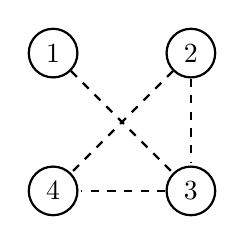
\begin{tikzpicture}[-,>=stealth,shorten >=1pt,auto,node distance=1.75cm, thick,main node/.style={scale=0.9,circle,draw,font=\sffamily\normalsize}]

                    \node[circle, draw] (1)[] {$1$};
                    \node[circle, draw] (2) [right of=1]{$2$};
                    \node[circle, draw] (3) [below of=2]{$3$};
                    \node[circle, draw] (4) [left of=3]{$4$};

                    \path[every node/.style={font=\sffamily\small}]
                        (1) edge[dashed] (3)
                        (2) edge[dashed] (3)
                        (2) edge[dashed] (4)
                        (3) edge[dashed] (4)
                        ;
                \end{tikzpicture}
            \end{tabular}

            &\quad&

            \begin{tabular}{c}
                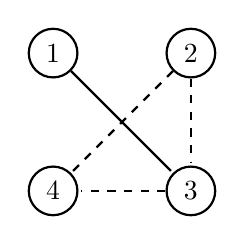
\begin{tikzpicture}[-,>=stealth,shorten >=1pt,auto,node distance=1.75cm, thick,main node/.style={scale=0.9,circle,draw,font=\sffamily\normalsize}]

                    \node[circle, draw] (1)[] {$1$};
                    \node[circle, draw] (2) [right of=1]{$2$};
                    \node[circle, draw] (3) [below of=2]{$3$};
                    \node[circle, draw] (4) [left of=3]{$4$};

                    \path[every node/.style={font=\sffamily\small}]
                        (1) edge (3)
                        (2) edge[dashed] (3)
                        (2) edge[dashed] (4)
                        (3) edge[dashed] (4)
                        ;
                \end{tikzpicture}
            \end{tabular}

        \end{tabular}

        \caption{Assuming that the tree queries $x_{1,2}$ and $x_{1,4}$, if we answer both queries with 0 then the tree has no way to decide the output until it queries $x_{1,3}$. Since answering with 0 would enable the tree to decide that the graph is disconnected, we are forced to answer 1. By repeating the process we can delay the decision until all bits are queried.}
    \end{figure}

    \newpage

    Given $n = 2^k$ for some $k$, consider the alternating AND-OR function $\mathrm{AND\text{-}OR} : \{0,1\}^n \to \{0,1\}$, defined as follows:
    \[\mathrm{AND\text{-}OR}(x_1, \ldots, x_{2^k}) = \soe{ll}{
        \mathrm{AO}(x_1, \ldots, x_{2^{k-1}}) \land \mathrm{AO}(x_{2^{k-1}+1}, \ldots, x_{2^{k}}) & \text{if $k>0$ and $k$ even} \\
        \mathrm{AO}(x_1, \ldots, x_{2^{k-1}}) \lor \mathrm{AO}(x_{2^{k-1}+1}, \ldots, x_{2^{k}}) & \text{if $k$ odd} \\
        x_i & \text{if $k = 0$}
    }\]

    It's easy to see that this function can be computed by a recursive circuit that alternates AND and OR gates. This circuit has depth $k$ and size $S(2^k) = 2 S \rbk{\frac{2^k}{2}} +1 = 2^k-1$. In query complexity, instead, we need a decision tree of depth exactly $2^k$, a result that can easily be proven by induction: when $k = 0$ we need 1 query, while when $k > 0$ we need to solve the two recursive steps, which both require $2^{k-1}$ bits by inductive hypothesis. This concludes that $D(\mathrm{AND\text{-}OR}) = 2^k = n$.

    Another technique to prove lower bounds for query complexity involves using some auxiliary complexity measures that are ensured to be at most equal to the query complexity of the function itself. The easiest complexity measure for this task is \textit{sensitivity}.

    \begin{frameddefn}{Sensitivity}
        Given a Boolean function $f : \{0,1\}^n \to \{0,1\}$ and an input $x \in \{0,1\}^n$, the \textbf{sensitivity of $f$ on $x$}, written as $s(f,x)$, is the number of bit positions $i$ such that flipping the $i$-th bit in $x$ chances the output.
        \[s(f,x) = \abs{\{i \mid f(x) \neq f(x \oplus e_i)\}}\]
        We define the \textbf{sensitivity} of $f$, written $s(f)$, as the maximum sensitivity of $f$ for any input $x \in \{0,1\}^n$.
    \end{frameddefn}

    Sensitivity is a very intuitive complexity measure. For instance, it's easy to see that the sensitivity of $\mathrm{AND}$, $\mathrm{OR}$ and $\mathrm{PARITY}$ is $n$ since for each bit we can find an input where flipping the bit changes the output. From the following lemma, we trivially get another easier proof of the fact that $D(\mathrm{AND}), D(\mathrm{OR}), D(\mathrm{PARITY}) = n$. 
    
    \begin{framedlem}{}
        Given a Boolean function $f : \{0,1\}^n \to \{0,1\}$, it holds that $s(f) \leq D(f)$
    \end{framedlem}

    \begin{proof}
        W.l.o.g. assume that $x_1, \ldots, x_{s(f)}$ are the sensitive bits of $f$. Since the output value depends on all of these bits, any decision tree computing $f$ will have to query all of these bits in order to decide the output correctly, concluding that $s(f) \leq D(f)$. 
    \end{proof}

    Given $n = k+2^k$, consider the \textit{address function} $\mathrm{ADDRESS} : \{0,1\}^n \to \{0,1\}$ that for each input $a_1, \ldots, a_{k}, x_1, \ldots, x_{2^k}$ returns the bit in $x_1, \ldots, x_{2^k}$ whose index is $a$, i.e. the bit $x_{a}$. By the very definition of this function, each of the first $k$ bits is clearly sensitive: for any $i \in [k]$, we can construct an input $a_1, \ldots, a_k, x_1, \ldots, x_{2^k}$ where $x_{a} = 1$ and $x_{a \oplus e_i} = 1-x_a$. Hence, we get that $D(\mathrm{ADDRESS}) \geq s(\mathrm{ADDRESS}) \geq k = \Omega(\log n)$.
    
    Moreover, it's easy to see that this function has a decision tree of depth $k+1$: we can query the first $k$ bits to find the address $a$ and then query the bit $x_{a}$, returning its value. Hence, the complete decision tree with $2^{k+1}-1$ nodes that queries each of the first $k$ bits and outputs the value $x_{a}$ suffices. This concludes that $D(\mathrm{ADDRESS}) \leq k+1 = O(\log n)$ and thus that $D(\mathrm{ADDRESS}) = \Theta(\log n)$, meaning that $\mathrm{ADDRESS} \in \mathsf{P}^{dt}$.
    


    \section{Certificate complexity}

    We saw how the class $\mathsf{P}^{dt}$ captures efficienct computations in decision trees, i.e. functions computable with a poly-log depth decision tree. We'll now focus on another complexity measure that can be viewed as the query complexity analog of the complex of verifiability, i.e. the \textit{certificate complexity }of a function.

    \begin{frameddefn}{0-certificates and 1-certificates}
        A \textbf{$b$-certificate} for a Boolean function $f: \{0,1\}^n \to \{0,1\}$, where $b \in \{0,1\}$, is a partial variable assignment $\rho$ such that $\forall x \in \{0,1\}^n$ compatible with $\rho$, meaning that each value set in $\rho$ is also set in $x$, it holds that $f(x) = b$.
    \end{frameddefn}

    In other words, a 0-certificate corresponds to a set of bits that once read ensures that the output value will be 0. Likewise, a 1-certificate corresponds to a set of bits that once read ensures that the output value will be 1. For any input $x$, we denote with $C^0(f.x)$ the length of the minimum 0-certificate for $x$. The analogous definition holds for $C^1(f,x)$.
    
    The \textbf{$b$-certificate complexity} of a function $f$, written as $C^b(f)$ is defined as the minimum value $k$ such that every input $x \in \{0,1\}^n$ has a $b$-certificate of size at most $k$. In other words, we have that:
    \[C^b(f) = \max_{x \in \{0,1\}^n : f(x) = b} C^b(f,x)\]
    
    The \textbf{certificate complexity} of a function $f$ is defined as $C(f) = \max(C^0(f), C^1(f))$.
    
    Consider the function $\mathrm{CONN}$ shown in the previous section. If the input graph $G$ is connected then a 1-certificate for such graph is a simple spanning tree of $G$, which has $m-1$ edges. Thus, the 1-certificate of $\mathrm{CONN}$ is $C^1(\mathrm{CONN}) \leq m-1$.
    
    When the input graph $G$ is disconnected, a 0-certificate for such graph is a simple cut of $G$, that is a set of edges whose non-existence forces $G$ to be disconnected. The number of edges in a cut is maximized when it partitions a complete graph $K_m$ into two connected subgraphs with $\frac{m}{2}$ nodes, which can be achieved by removing half of the edges incident to each node in one of the two halves (the other half will also have half of its edges removed as a byproduct of this process). The decision tree the 0-certificate complexity of $\mathrm{CONN}$ is thus $C^0(\mathrm{CONN}) \leq \rbk{\frac{m}{2}}^2 = \frac{m^2}{4}$. Moreover, we notice that some graphs such as the graph consisting of two disjoint cliques of size $\frac{m}{2}$ do not have smaller 0-certificate, hence $C^0(\mathrm{CONN}) = \frac{m^2}{4}$. This concludes that $C(\mathrm{CONN}) = \frac{m^2}{4}$.

    \begin{framedprop}{}
        For any Boolean function $f : \{0,1\}^n \to \{0,1\}$, it holds that $s(f) \leq C(f)$ and that $C^0(f), C^1(f) \leq D(f)$
    \end{framedprop}

    \begin{proof}
        Let $x$ be an input with maximum sensitivity, i.e. $s(f) = s(f,x)$. Let $b$ be such that $f(x) = b$. We notice that if $(x \oplus e_i) \neq f(x)$ for $i \in [n]$, then $i$ must be present in every certificate for $x$, concluding that $s(f) = s(f, x) \leq C^b(f, x) \leq C^b(f) \leq C(f)$.

        Let now $y$ be an input with maximum 0-certificate bits, i.e. $C(f) = C(f,y)$. Let $b$ be such that $f(y) = b$. Given a decision tree $T$ for $f$ with depth $D(f)$, the partial assignment given by the path determined by $x$ on $T$ is clearly $b$-certificate for $f$, and it has size at most $D(f)$. Hence, we conclude that $C(f) = C(f,y) \leq D(f)$.
    \end{proof}

    Intuitively, we define $\mathsf{NP}^{dt}$ as the class of functions who have a poly-log 1-certificate complexity, while $\mathsf{coNP}^{dt}$ is the class of functions who have a poly-log 0-certificate complexity. The previous lemma clearly implies that $\mathsf{P}^{dt} \subseteq \mathsf{NP}^{dt} \cap \mathsf{coNP}^{dt}$. In the query complexity world we are capable of showing that this inclusion also holds in the other direction (this fact comes from the following theorem), meaning that $\mathsf{P}^{dt} = \mathsf{NP}^{dt} \cap \mathsf{coNP}^{dt}$. Some believe that this should also hold for the standard Turing machine model, however there is not enough evidence to believe this.

    \begin{framedlem}{}
        Given a function $g : \{0,1\}^n \to \{0,1\}$, every 0-certificate $\rho_0$ of $g$ must share at least one variable with every 1-certificate $\rho_1$ of $g$ and this variable must assume different values in $\rho_0$ and $\rho_1$.
    \end{framedlem}

    \begin{proof}
        By way of contradiction, suppose that $\rho_0$ and $\rho_1$ share no variables. Then, we can build a decision tree that has a path that first queries the bits of $\rho_0$ and then queries the bits of $\rho_1$. By definition, this path must guarantee that the output is both 0 and 1 at the same time, which is impossible. Hence, there must be at least one shared variable.

        Again, by way of contradiction suppose that there is no shared variable that aassumes a different value in the two certificates. Then, we can build a decision tree with a path that first queries each bit of the intersection and then queries the remaining bits of $\rho_0$ and $\rho_1$. Again, here the output would be guaranteed to be both 0 and 1 at the same time, which is impossible. 
    \end{proof}

    \newpage

    \begin{framedthm}{}
        For any Boolean function $f : \{0,1\}^n \to \{0,1\}$, it holds that $D(f) \leq C^0(f) \cdot C^1(f)$
    \end{framedthm}

    \begin{proof}

        Using the previous lemma, we inductively construct a decision tree with depth at most $C^0(f) \cdot C^1(f)$. If $C^1(f) = 0$, the single node decision tree labeled with 1 suffices since no bits have to be queried.
        
        Suppose now that $C^1(f) > 0$. Let $S_f^0$ be the set of 0-certificate of $f$ with length at most $C^0(f)$. Pick a 0-certificate $\rho_f^0 \in S_f^0$. Construct the complete decision tree whose paths query the variables in $\rho_f^0$. This decision tree has at most $2^{C^0(f)-1}$ paths. Let $\sigma_i$ be the partial assignment corresponding to the $i$-th path of this complete tree. We observe that for only one of the paths it will hold that $\sigma_i = \rho_f^0$. We label the leaf of this path with 0 since $\rho_f^0$ is a 0-certificate.

        For every path of the complete tree such that $\sigma_i \neq \rho_f^0$, we consider the restricted function $f_{\mid \sigma_i}$. Since $\sigma_i$ may not be inside $S_f^0$ and $f_{\mid \sigma_i}$ is a restriction of $f$, we have that $C^0(f_{\mid \sigma_i}) \leq C^0(f)$. Moreover, by the previous lemma, we know that any 1-certificate of $f$ must share at least one different valued variable with $\rho_f^0$ and each assigment $\sigma_i$ as at least one bit different from $\rho_f^0$, each 1-certificate already has a variable compatible with $\sigma_i$, meaning that $C^1(f_{\mid \sigma_i}) \leq C^1(f)-1$. By inductive hypothesis, for each other path $\sigma$ there is a decision tree $T_{\sigma_i}$ that computes $f_{\mid \sigma_i}$ with depth at most $C^0(f_{\mid \sigma_i}) \cdot C^1(f_{\mid \sigma_i}) \leq C^0(f) \cdot (C^1(f)-1)$.
        
        By attaching each tree $T_{\sigma_i}$ at the end of each path $\sigma_i \neq \rho_f^0$ of the full decision tree, we get the final decision tree that computes $f$. Since each path $\sigma_i$ has length at most $C^0(f)$, the final decision tree has depth at most $C^0(f) + C^0(f) \cdot (C^1(f)-1) = C^0(f) \cdot C^1(f)$.
    \end{proof}

    \begin{figure}[H]
        \centering

        \includegraphics[width=\textwidth]{images/dtrees_cert.pdf}

        \caption{Tree constructed in proof of the previous theorem assuming the picked 0-certificate $\rho_f^0$ contains $x_1 = 0, x_4 = 1, x_5 = 0$}
        \label{proof_tree}
    \end{figure}

    \newpage

    \section{Randomized decision trees}

    After discussing deterministic and \curlyquotes{non-deterministic} complexities in decision trees through query complexity and certificate complexity, it naturally follows to discuss randomized complexity in decision trees. In a \textbf{randomized decision tree}, the choice of which input location to query is  determined probabilistically: some nodes of the tree can flip a coin that choses the next bit to be queried. We will consider randomized trees that always output the right answer but use randomization to possibly speedup their expected cost -- think of this as the query complexity equivalent of the class $\mathsf{ZPP}$.

    \begin{figure}[H]
        \centering

        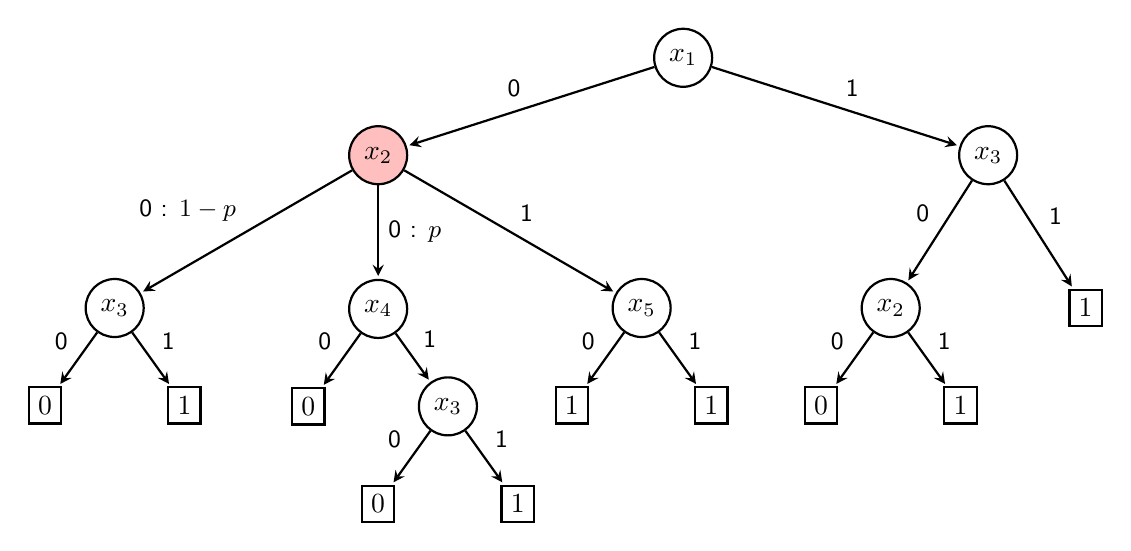
\begin{tikzpicture}[->,>=stealth,shorten >=1pt,auto,node distance=1.75cm, thick,main node/.style={scale=0.9,circle,draw,font=\sffamily\normalsize}]

            \node[circle, draw] (1)[] {$x_1$};

            \node[circle, draw, fill=pink] (2) [below left of=1, xshift=-75, ]{$x_2$};
            \node[circle, draw] (3) [below right of=1, xshift=75, ]{$x_3$};

            \node[circle, draw] (4) [below left of=2, xshift=-60, yshift=-20]{$x_3$};
            \node[circle, draw] (x) [below of=2, yshift=14.25-20]{$x_4$};
            \node[circle, draw] (5) [below right of=2, xshift=60, yshift=-20]{$x_5$};
            \node[circle, draw] (6) [below left of=3, yshift=-20]{$x_2$};
            \node[rectangle, draw] (7) [below right of=3, yshift=-20]{$1$};

            \node[rectangle, draw] (8) [below left of=4, xshift=10]{$0$};
            \node[rectangle, draw] (9) [below right of=4, xshift=-10]{$1$};
            \node[rectangle, draw] (8x) [below left of=x, xshift=10]{$0$};
            \node[circle, draw] (9x) [below right of=x, xshift=-10]{$x_3$};
            \node[rectangle, draw] (10) [below left of=5, xshift=10]{$1$};
            \node[rectangle, draw] (11) [below right of=5, xshift=-10]{$1$};
            \node[rectangle, draw] (12) [below left of=6, xshift=10]{$0$};
            \node[rectangle, draw] (13) [below right of=6, xshift=-10]{$1$};
            \node[rectangle, draw] (8y) [below left of=9x, xshift=10]{$0$};
            \node[rectangle, draw] (9y) [below right of=9x, xshift=-10]{$1$};

            \path[every node/.style={font=\sffamily\small}]
                (1) edge[swap]  node{0} (2)
                (1) edge node{1}(3)

                (2) edge[swap]  node{0 : $1-p$} (4)
                (2) edge[]  node{1}(5)

                (3) edge[swap]  node{0} (6)
                (3) edge  node{1}(7)
                            
                (4) edge[swap]  node{0} (8)
                (4) edge  node{1}(9)

                (5) edge[swap]  node{0} (10)
                (5) edge[]  node{1}(11)

                (6) edge[swap]  node{0} (12)
                (6) edge  node{1}(13)

                (2) edge node{0 : $p$} (x)
                (x) edge[swap] node{0} (8x)
                (x) edge node{1} (9x)
                (9x) edge[swap] node{0} (8y)
                (9x) edge node{1}(9y)
                ;
        \end{tikzpicture}

        \caption{An example of a randomized decision tree. When the answer to the pink query is 0, the tree choses with probability $p$ and $1-p$ which is the next query.}
    \end{figure}

    We notice that this decision tree corresponds to two possible decision trees, one chosen with probability $p$ and the other chosen with probability $1-p$. In fact, each randomized decision tree for $f$ can be viewed as \textbf{probability distribution} over all the deterministic decision trees for $f$, and vice versa. This allows us to give an easier definition of randomized complexity.

    In particular, we notice that even though $\mathcal{T}_f$ contains an finite number of decision trees (if we assume that queries cannot be repeated on the same path), the number of possible tree is still exponential with respect to the input size. However, this is no problem for us: since we're working with probability distributions, we can restrict our interest to a smaller set of decision trees and assign the probability 0 to all the other decision trees.
    
    We define $\mathcal{P}_f$ as the set of probability distribuitions over $\mathcal{T}_f$. The \textit{cost} of a distribuition $P \in \mathcal{P}_f$ for an input $x$, written as $\mathrm{cost}(P,x)$, is the expected cost of the computatation $T(x)$ of any decision tree $T$ inside $P$.
    \[\mathrm{cost}(P,x) = \Exp_{T \in_R P}[\mathrm{cost}(T,x)]\]
    
    The \textbf{randomized query complexity} of a function $f$, denoted as $R(f)$, is defined as the minimum cost of a decision tree distribution for $f$ over all inputs.
    \[R(f) = \min_{P \in \mathcal{P}_f} \max_{x \in \{0,1\}^n} \mathrm{cost}(P,x)\]

    In other words, the randomized query complexity expresses how well the best possible
    probability distribution of trees will do on average against the worst possible input.

    For instance, consider the \textit{majority funciton} on three bits $\mathrm{MAJ}(x_1, x_2, x_3)$ which outputs 1 when the majority of the bits is set to 1, 0 otherwise. In standard query complexity, we can easily compute this function through the following decision tree.

    \begin{figure}[H]
        \centering

        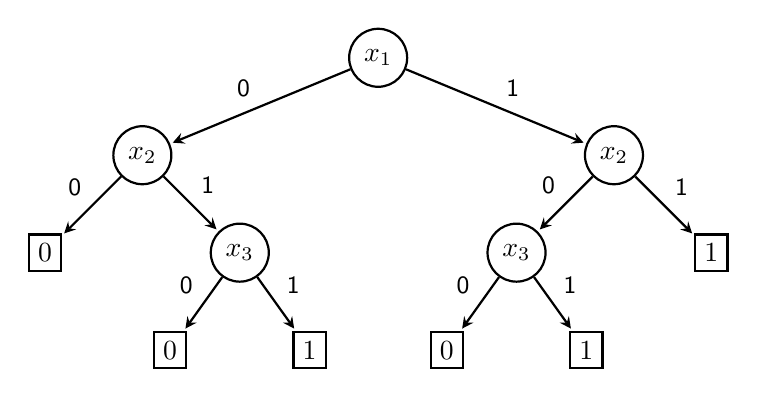
\begin{tikzpicture}[->,>=stealth,shorten >=1pt,auto,node distance=1.75cm, thick,main node/.style={scale=0.9,circle,draw,font=\sffamily\normalsize}]

            \node[circle, draw] (1)[] {$x_1$};

            \node[circle, draw] (2) [below left of=1, xshift=-50, ]{$x_2$};
            \node[circle, draw] (3) [below right of=1, xshift=50, ]{$x_2$};

            \node[rectangle, draw] (4) [below left of=2, ]{$0$};
            \node[circle, draw] (5) [below right of=2, ]{$x_3$};
            \node[circle, draw] (6) [below left of=3, ]{$x_3$};
            \node[rectangle, draw] (7) [below right of=3]{$1$};

            \node[rectangle, draw] (10) [below left of=5, xshift=10]{$0$};
            \node[rectangle, draw] (11) [below right of=5, xshift=-10]{$1$};
            \node[rectangle, draw] (12) [below left of=6, xshift=10]{$0$};
            \node[rectangle, draw] (13) [below right of=6, xshift=-10]{$1$};

            \path[every node/.style={font=\sffamily\small}]
                (1) edge[swap, ]  node{0} (2)
                (1) edge node{1}(3)

                (2) edge[swap]  node{0} (4)
                (2) edge[]  node{1}(5)

                (3) edge[swap]  node{0} (6)
                (3) edge  node{1}(7)

                (5) edge[swap]  node{0} (10)
                (5) edge[]  node{1}(11)

                (6) edge[swap]  node{0} (12)
                (6) edge  node{1}(13)
                ;
        \end{tikzpicture}

        \caption{Decision tree computing $\mathrm{MAJ}$ on 3 bits.}
    \end{figure}

    Meaning that we require at most 3 queries. Through an adversarial argument or sensitivity, we can easily show that this number of queries is also a lower bound, concluding that $D(\mathrm{MAJ}_3) = 3$.
    
    Let $P$ be a probability distribuition over $\mathcal{T}_{\mathrm{MAJ}_3}$, defined as follows:
    \begin{itemize}
        \item Each decision tree with structure equal to the one in the previous picture but where the order of the queries is \textit{permuted} gets the same probability. Since the number of permutations of 3 bits is $3! = 6$, each of these trees gets probability $\frac{1}{6}$.
        \item Every other decision tree gets probability 0
    \end{itemize}
    
    It's easy to see that each of the permutated trees will \curlyquotes{favor} one or more input, meaning that they require a lower number of queries to be computed. For instance, the tree that queries the bits using the order $x_2, x_3, x_1$ will favor the inputs where $x_2$ and $x_3$ are equal, i.e. the inputs $000, 001, 110, 111$, while the tree that queries $x_1, x_3, x_2$ will favor the inputs where $x_1$ and $x_3$ are equal.

    For each of the permuted trees, the probability that the first two bits that it queries are equal is $\frac{1}{3}$. Hence, we have that:
    \[\max_{x \in \{0,1\}^n} \Exp_{T \in_R P}[\mathrm{cost}(T,x)] = 2 \cdot \frac{1}{3} + 3 \cdot \frac{2}{3} = \frac{8}{3}\]
    
    Since we do not know if this distribuition is the best possible one, we can only conclude that $R(\mathrm{MAJ}_3) \leq \frac{8}{3}$.

    \newpage

    \begin{framedthm}{}
        For any Boolean function $f : \{0,1\}^n \to \{0,1\}$, it holds that $C(f) \leq R(f) \leq D(f)$.
    \end{framedthm}

    \begin{proof}
        By linearity of the expected value operator and the definition of certificate complexity, we get that:
        \[\begin{split}
            R(f) &= \min_{P \in \mathcal{P}_f} \max_{x \in \{0,1\}^n} \Exp_{T \in_R P}[\mathrm{cost}(T,x)]\\
            & \geq \min_{P \in \mathcal{P}_f} \max_{x \in \{0,1\}^n} \Exp_{T \in_R P}[C(f,x)]\\
            & = \min_{P \in \mathcal{P}_f} \max_{x \in \{0,1\}^n} C(f,x)\\
            & = \min_{P \in \mathcal{P}_f} C(f)\\
            & = C(f)\\
        \end{split}\]

        Since any decision tree that decides $f$ lies inside $\mathcal{T}_f$, any $P \in \mathcal{P}_f$ will also have the optimal tree inside it. This concludes that $R(f) \leq D(f)$ since the optimal tree gives an upper bound on the expected value.
    \end{proof}

    To study randomized complexity, we have to also study \textit{distributional complexity}. In the former, we're interested in the expected cost over a random computation for the worst input. In the latter, instead, we're interested in the expected cost over the best deterministic computation for a random input.

    Let $\mathcal{X}_n$ be the set of probability distributions over $\{0,1\}^n$. The \textit{cost} of a distribuition $X \in \mathcal{X}_n$ for a decision tree $T$, written as $\mathrm{cost}(T,X)$, is the expected cost of the computatation $T(x)$ of any input $x$ inside $X$.
    \[\mathrm{cost}(T,X) = \Exp_{x \in_R X}[\mathrm{cost}(T,x)]\]

    The \textbf{distributional complexity} of a function $f$, denoted as $\mathcal{D}(f)$, is defined as the maximum cost of an input distribution for $f$ over all decision trees in $\mathcal{T}_f$.
    \[\mathcal{D}(f) = \max_{X \in \mathcal{X}_n} \min_{T \in \mathcal{T}_f} \mathrm{cost}(T,X)\]

    The distributional complexity easily gives us a lower bound on randomized complexity: by analyzing the average performance of the worst possible input distribuition on all decision trees, we get informations on the average performance of the best decision tree distrubution for all inputs, since every distribution will be lower bounded.

    \begin{framedlem}[label={distr_rand}]{}
        For any Boolean function $f : \{0,1\}^n \to \{0,1\}$, it holds that $\mathcal{D}(f) \leq R(f)$.
    \end{framedlem}

    \begin{proof}
        First, we notice that for any input distribution $X \in \mathcal{X}_n$ (even the worst one)  it holds that:
        \[\min_{T \in \mathcal{T}_f} \Exp_{x \in_R X}[\mathrm{cost}(T,x)] \leq \Exp_{\substack{x \in_R X\\T \in_R \mathcal{T}_f}}[\mathrm{cost}(T,x)]\]

        Similarly, for any fixed decision tree distribuition $P \in \mathcal{P}_f$ (even the best one)  it holds that:
        \[\max_{x \in \{0,1\}^n} \Exp_{T \in_R P}[\mathrm{cost}(T,x)] \geq \Exp_{\substack{x \in_R X\\T \in_R \mathcal{T}_f}}[\mathrm{cost}(T,x)]\]

        Hence, we get that:
        \[\begin{split}
            \mathcal{D}(f) &= \max_{X \in \mathcal{X}_n} \min_{T \in \mathcal{T}_f} \Exp_{x \in_R X}[\mathrm{cost}(T,x)] \\
            &\leq \max_{X \in \mathcal{X}_n} \Exp_{\substack{x \in_R X\\T \in_R \mathcal{T}_f}}[\mathrm{cost}(T,x)] \\
            &\leq \min_{P \in \mathcal{P}_f} \max_{x \in_R \{0,1\}^n} \Exp_{T \in_R P}[\mathrm{cost}(T,x)]\\
            & = R(f)
        \end{split}\]
    \end{proof}

    This lemma gives us an easy way to prove lower bounds on randomized complexity. In particular, we can pick an adversarial distribuition that performs badly on every decision tree in order to get a lower bound for $\mathcal{D}(f)$, which is also a lower bound for $R(f)$.

    To show how this works, consider again the majority function on 3 bits $\mathrm{MAJ}_3$. We already showed that $R(\mathrm{MAJ}_3) \leq \frac{8}{3}$. We'll now show that this bound also holds in the other direction. Given the set of inputs $\{0,1\}^3 = \{000,001,010,011,100,101,110,111\}$, let $X$ be the input distribution that assigns probability $0$ to the inputs $000$ and $111$, while all the other inputs get assigned probability $\frac{1}{6}$.
    
    For each input $x \in X - \{000,111\}$, the number of decision trees that favor $x$, i.e. those for which 2 queries on $x$ suffice, is the same as those that are not favorable to $x$, those that require 3 queries. In other words, an input is favored by a decision tree with probability $\frac{2}{6}$ (one if the two bits are 0 and one if they are 1), meaning that:
    \[\min_{T \in \mathcal{T}_f} \Exp_{x \in_R X}[\mathrm{cost}(T,x)] = 2 \cdot \frac{2}{6} + 3 \cdot \frac{4}{6} = \frac{8}{3}\]

    Since we don't know if this distribuition is the worst possible one, we can only conclude that $\frac{8}{3} \leq \mathcal{D}(\mathrm{MAJ}) \leq R(\mathrm{MAJ})$, which suffices to show that $\mathcal{D}(\mathrm{MAJ}) = R(\mathrm{MAJ}) = \frac{8}{3}$.

    \newpage

    \section{Zero-sum games and Yao's min-max principle}

    In the previous section we discussed how distributional complexity acts as a lower bound on randomized complexity. In this section, we will show that these two complexity measures are actually equal to each other. In particular, we will prove this through an even stronger result known as \textbf{Yao's min-max principle} (or \textit{Yao's min-max lemma}) \cite{yao}, which proves that this equiality is true not only for decision trees but also for \textbf{every deterministic algorithm}.
    
    Yao's min-max principle is considered one of the most important results in computer science, showing that proving limitations on the performance of randomized algorithms can be reduced to finding a probability distribution on inputs that is difficult for deterministic algorithms, while inferring that randomized algorithms have the same limitation on their worst case performance.
    
    To prove Yao's result, we first have to discuss about \textbf{game theory} and Von Neumann's famous \textbf{minimax theorem}. In particular, we focus on 2-player games. Any 2-player game can be modeled by an $m \times n$ matrix $A$ of real numbers. Each round consists of only two moves: one by the first player and one by the second player. The first player -- the \textit{row player} -- picks an index $i \in [m]$, while the second player -- the \textit{column player} -- picks an index $j \in [n]$. The \textit{outcome} of the round is the entry $a_{i,j}$ of the matrix $A$ and it corresponds to a tuple $(b,c)$, where $b$ and $c$ respectively correspond to how much the first and the second player win (a negative value represents that they lose points).

    To better understand how a 2-player game works, we consider the \textit{parity game}: each player chooses the value of a bit. If the parity of such bits is even, the even player wins. Otherwise, the odd player wins. In each round, the player pays 1 point to the winning player. In other words, given the outcome function $f$, we have that:
    \[f(x,y) = \soe{ll}{
        (+1, -1) & \text{if } x \xor y = 0 \\
        (-1, +1) & \text{if } x \xor y = 1 \\
    }\]

    \begin{figure}[H]
        \centering
        \begin{tabular}{cc|cc}
            \multirow{2}{*}{} & \multicolumn{1}{c}{} & \multicolumn{2}{c}{Odd} \\
            &  & \multicolumn{1}{c}{0} & \multicolumn{1}{c}{1} \\
            \cline{2-4}
            \multirow{2}{*}{Even} & 0 & $(+1, -1)$ & $(-1, +1)$\\
             & 1 & $(-1, +1)$ & $(+1, -1)$\\
        \end{tabular}

        \caption{2-player game representation of the parity game.}
    \end{figure}

    In particular, we notice that in the parity game the points won by a player correspond to the points lost by the other player. When this happens, we say that the game is a \textbf{zero-sum game}. The name comes from the fact that the sum between the win of one party and the loss of the other always equals zero. These games also allow us to restrict our attention to the win or loss of a player, instead of both. For instance, since the even player moves first, we can restrict our attention on the points won or loss by them.

    \begin{figure}[H]
        \centering
        \begin{tabular}{cc|cc}
            \multirow{2}{*}{} & \multicolumn{1}{c}{} & \multicolumn{2}{c}{Odd} \\
            &  & \multicolumn{1}{c}{0} & \multicolumn{1}{c}{1} \\
            \cline{2-4}
            \multirow{2}{*}{Even} & 0 & $+1$ & $-1$\\
             & 1 & $-1$ & $+1$\\
        \end{tabular}

        \caption{Zero-sum game representation of the parity game.}
    \end{figure}

    The even player wants to maximize the outcome of the round, while the odd player wants to minimize such outcome. More generally, in each zero-sum game one of the two players assumes the role of \textbf{minimizer}, while the other assumes the role of \textbf{maximizer}.

    Clearly, the order in which players make their moves is important. For instance, if the eeven player starts with 1, the odd player will respond with 0 in order to win. But what happens if we allow the players to use \textit{randomized strategies}?

    A randomized strategy for the column player can be viewed as distribution over the columns, that is a vector $x$ inside a \textit{standard simplex} $X \subseteq \{0,1\}^n$, which is subset whose vectors' components sum to zero:
    \[X = \cbk{x \in \{0,1\}^n \left | \sum_{k = 1}^n x_k = 1 \right .}\]
    
    Likewise, the row player chooses a distribution $y$ from a standard simplex $Y \subseteq \{0,1\}^m$.

    The outcome is the \textit{expectation} of $a_{i,j}$ for $i$ chosen from $x$ and $j$ chosen from $y$, i.e. $a_{i,j} = \Exp_{\substack{i \in_R x\\j \in_R y}} f(i,j)$. If we think of $x$ and $y$ as vectors then $x^TAy = \Exp_{\substack{i \in_R p\\j \in_R q}} f(i,j)$. Moreover, we notice that the function $g(x,y)$ defined as $g(x,y) = \Exp_{\substack{i \in_R p\\j \in_R q}} f(i,j)$ is a \textit{bilinear function}, meaning that it is linear in both variables.

    Von Neumann's Minimax theorem \cite{von_neumann} shows that, surprisingly, if we allow the players to use randomized strategies then the order of play is actually \textbf{irrelevant}.

    \begin{framedthm}{Von Neumann's Minimax theorem}
        Given two standard simplices $X \subseteq \{0,1\}^n, Y \subseteq \{0,1\}^m$ and a bilinear function $g : \{0,1\}^{n+m} \to \R$ described by a matrix $A$, it holds that:
        \[\min_{x \in X} \max_{y \in Y} x^TAy = \max_{y \in Y} \min_{x \in X} x^TAy\]

    \end{framedthm}
    \begin{proof} Omitted. \end{proof}

    We're now set to discuss Yao's min-max lemma. Let $\mathcal{A}$ be a class of deterministic algorithms (Turing machines, decision trees, $\ldots$). Let $\mathcal{A}_f$ denote the subset of $\mathcal{A}$ containing the algorithms that compute a function $f$. The sets $\mathcal{P}_f$ and $\mathcal{X}_n$ are respectively the set of distribuitions over $\mathcal{A}_f$ and $\{0,1\}^n$. For each $A \in \mathcal{A}_f$ and each input $x$, let $\mathrm{cost}(A,x)$ denote the \textit{cost} (running time, used space, query complexity, $\ldots$) of the computation $A(x)$.

    \begin{framedthm}{Yao's min-max principle}
        Given a Boolean function $f$ and a class of algorithms $\mathcal{A}$, it holds that:
        \[\max_{X \in \mathcal{X}_n} \min_{A \in \mathcal{A}_f} \Exp_{x \in_R X}[\mathrm{cost}(A,x)] = \min_{P \in \mathcal{P}_f} \max_{x \in \{0,1\}^n} \Exp_{A \in_R P}[\mathrm{cost}(A,x)]\]
    \end{framedthm}

    \begin{proof}
        Proceeding the same way as in \Cref{distr_rand}, we can easily show that:
        \[\max_{X \in \mathcal{X}_n} \min_{A \in \mathcal{A}_f} \Exp_{x \in_R X}[\mathrm{cost}(A,x)] \leq \min_{P \in \mathcal{P}_f} \max_{x \in \{0,1\}^n} \Exp_{A \in_R P}[\mathrm{cost}(A,x)]\]

        To prove that the other inequality also holds, we notice that:
        \[\min_{P \in \mathcal{P}_f} \max_{x \in \{0,1\}^n} \Exp_{A \in_R P}[\mathrm{cost}(A,x)]\leq \min_{P \in \mathcal{P}_f} \max_{X \in \mathcal{X}_n} \Exp_{\substack{x \in_R X\\A \in_R P}}[\mathrm{cost}(A,x)]\]

        Since the expected value is a multilinear operator and both $\mathcal{P}_f$ and $\mathcal{X}_f$ are standard simplices, we can apply Von Neumann's Minimax theorem:
        \[\begin{split}
        \min_{P \in \mathcal{P}_f} \max_{x \in \{0,1\}^n} \Exp_{A \in_R P}[\mathrm{cost}(A,x)] &\leq \min_{P \in \mathcal{P}_f} \max_{X \in \mathcal{X}_n} \Exp_{\substack{x \in_R X\\A \in_R P}}[\mathrm{cost}(A,x)] \\
        &= \max_{X \in \mathcal{X}_n} \min_{P \in \mathcal{P}_f}  \Exp_{\substack{x \in_R X\\A \in_R P}}[\mathrm{cost}(A,x)] \\
        & \leq \max_{X \in \mathcal{X}_n} \min_{A \in \mathcal{A}_f} \Exp_{x \in_R X}[\mathrm{cost}(A,x)]
        \end{split}\]
    \end{proof}

    \begin{framedcor}{}
        For any Boolean function $f : \{0,1\}^n \to \{0,1\}$, it holds that $\mathcal{D}(f) = R(f)$.
    \end{framedcor}

    \chapter{Communication complexity}

    \section{Two-party protocols}

    Up to this chapter, we have seen how 2-player games come in handy in many situations, such as interective proofs and zero-sum games. We'll now discuss another application of such concept in \textit{communication complexity}. This branch of computational complexity focuses on number of bits that must be communicated to achieve a common task. Communication complexity finds crucial applications in the context of VLSI circuit design, streaming algorithms and clusters. 

    Suppose that we have two players who want to cooperate in order to compute a function. To reach their goal, the two players must carry out separate computations, communicating the result to the other party in a pre-defined sequence of steps. This idea serves as groundwork for a definition of \textbf{protocols}, i.e. algorithms that dictate such alternations between computation and communications. The setup is similar to interactive proofs: the two players compute a smaller task and communicate the result to the other player. However, in this case we have \underline{no randomness}. Instead of studying the running time of the computation, we're interested in studying the \textit{number of bits} exchanged by the two parties. To differentiate these types of communications from those of interactive proofs, the two players will be referred to as Alice and Bob.

    \begin{frameddefn}{Two-party protocol}
        A \textbf{$t$-round two-party protocol} $\Pi$ is a sequence of $t$ functions $P_1, \ldots, P_t : \{0, 1\}^* \to \{0, 1\}^*$ whose execution on inputs $x, y \in \{0,1\}^n$ is defined iteratively as follows: at the $i$-th round, if $i$ is odd then Alice computes $p_i = P_i(x, p_1, \ldots, p_{i-1})$ and sends $p_i$ to Bob, while if $i$ is even then Bob computes $p_i = P_i(y, p_1, \ldots, p_{i-1})$ and sends $p_i$ to Alice. 

        A Boolean function $f : \{0, 1\}^{2n} \to \{0, 1\}$ is said to be computed by a protocol $\Pi$ if for every input $x,y \in \{0,1\}^{n}$ the last message sent is equal to the output of $f$, that is $p_t = f(x,y)$.
    \end{frameddefn}
    
    \begin{figure}[H]
        \centering

        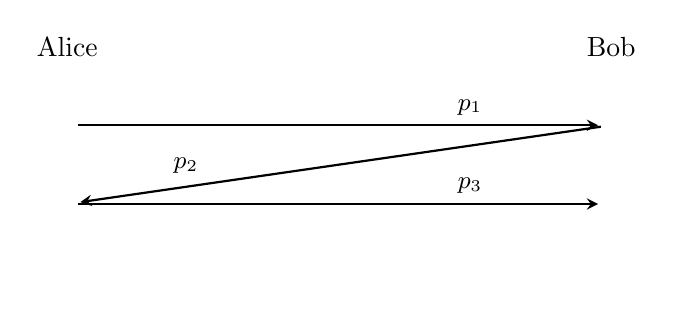
\begin{tikzpicture}[->,>=stealth,shorten >=1pt,auto,node distance=1cm,thick,main node/.style={scale=0.8,circle,draw,font=\sffamily\normalsize}]
            \node[] (1) []{$\mathrm{Alice}$};
            \node[] (2) [left of = 1, xshift = 225]{$\mathrm{Bob}$};

            \node[] (3) [below of = 1]{};
            \node[] (4) [below of = 2]{};

            \node[] (5) [below of = 3]{};
            \node[] (6) [below of = 4]{};

            \node[] (7) [below of = 5]{};
            \node[] (8) [below of = 6]{};

            \path[every node/.style={font=\sffamily\small}]
                (3) edge[near end] node{$p_1$} (4)
                (4) edge[swap, near end] node{$p_2$} (5)
                (5) edge[near end] node{$p_3$} (6)
                ;
        \end{tikzpicture}

        \caption{Computation in an $3$ round two-party protocol}
    \end{figure}

    The communication complexity of a protocol $\Pi$ is the maximum number of bits communicated for any input, i.e. the maximum value of $\abs{p_1} + \ldots + \abs{p_t}$ over all inputs $x, y \in \{0, 1\}^{n}$. The \textbf{communication complexity} of a Boolean funcion $f$, denoted by $CC(f)$ is the minimum complexity over all the protocols that compute $f$.
    
    Protocols can also be described as a \textbf{rooted binary tree} (similar to \textit{decision trees}) whose leaves are associated with outputs and internal nodes are owned by either Alice or Bob, where the owner of $v$ is noted by $\mathrm{owner}(v)$. Each leaf is labeled with an output $b \in \{0,1\}$. Each internal node $v$ is associated to a function $f_v : \{0,1\}^n \to \{0,1\}$ that dictates how the computation proceeds.

    When given the inputs $x,y \in \{0,1\}^n$, the protocol computes the associated function of the current node (starting from the root), proceeding on the left child if the output is 0 and on the right child if the output is 1. When a leaf is reached, the protocol returns the associated output. The output of the protocol for a given input $(x,y)$ is denoted with $\Pi(x,y)$. A function $f$ is said to be computed by the protocol $\Pi$ if for all inputs $(x,y)$ it holds that $f(x,y) = \Pi(x,y)$.

    Here, the complexity of protocols is measured in terms of the \textit{depth} of the tree. The \textbf{communication complexity} of a function $f$ is defined as the depth of the smallest protocol that computes $f$, corresponding to the minimal number of bits that must be communicated by Alice and Bob to compute $f$ for all possible inputs.

    \begin{figure}[H]
        \centering

        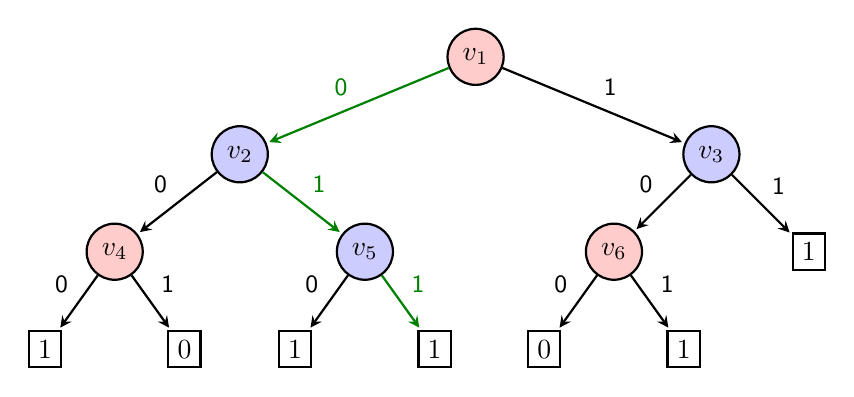
\begin{tikzpicture}[->,>=stealth,shorten >=1pt,auto,node distance=1.75cm, thick,main node/.style={scale=0.9,circle,draw,font=\sffamily\normalsize}]

            \node[circle, draw] (1)[fill=red!20] {$v_1$};

            \node[circle, draw] (2) [below left of=1, xshift=-50, fill=blue!20]{$v_2$};
            \node[circle, draw] (3) [below right of=1, xshift=50, fill=blue!20]{$v_3$};

            \node[circle, draw] (4) [below left of=2, xshift=-10, fill=red!20]{$v_4$};
            \node[circle, draw] (5) [below right of=2, xshift=10, fill=blue!20]{$v_5$};
            \node[circle, draw] (6) [below left of=3, fill=red!20]{$v_6$};
            \node[rectangle, draw] (7) [below right of=3]{$1$};

            \node[rectangle, draw] (8) [below left of=4, xshift=10]{$1$};
            \node[rectangle, draw] (9) [below right of=4, xshift=-10]{$0$};
            \node[rectangle, draw] (10) [below left of=5, xshift=10]{$1$};
            \node[rectangle, draw] (11) [below right of=5, xshift=-10]{$1$};
            \node[rectangle, draw] (12) [below left of=6, xshift=10]{$0$};
            \node[rectangle, draw] (13) [below right of=6, xshift=-10]{$1$};

            \path[every node/.style={font=\sffamily\small}]
                (1) edge[swap, color=Green]  node{0} (2)
                (1) edge node{1}(3)

                (2) edge[swap]  node{0} (4)
                (2) edge[color=Green]  node{1}(5)

                (3) edge[swap]  node{0} (6)
                (3) edge  node{1}(7)
                                        
                (4) edge[swap]  node{0} (8)
                (4) edge  node{1}(9)

                (5) edge[swap]  node{0} (10)
                (5) edge[color=Green]  node{1}(11)

                (6) edge[swap]  node{0} (12)
                (6) edge  node{1}(13)
                ;
                    \end{tikzpicture}

        \caption{An example of a protocol of size 13 and depth 3 where the red nodes are owned by Alice and the blue nodes are owned by Bob. The green path shows the computation given by $f_{v_1}(x) = 0$, $f_{v_2}(y) = 1$ and $f_{v_5}(y) = 1$ for the input $(x,y)$.}
    \end{figure}

    \newpage

    In other words, instead of considering the outputs of the previous computations as additional input bits, we can just consider how the computation proceeds for the very same outputs. On first glance, decision trees and protocols may look like the same computational model through this representation. However, we have two fundamental differences:
    \begin{itemize}
        \item Alice and Bob know their imput from the start of the computation and they don't have to make some queries in order to discover it.
        \item The internal functions associated to each node can be as strong as we like and they are not limited to correspond to a single bit of the input. 
        \item In decision trees we're intersted in how many bits of the input we must know, while in protocols we're interested in how many bits we have to communicate.
    \end{itemize}

    It's easy to see that for every function $f$ it holds that $CC(f) \leq n+1$ since any function can be computed by the \textit{trivial protocol} where Alice sends all the bits of her input to the other party, who then computes the whole function $f(x,y)$ alone and communicates the result. However, since the power of the two parties is \textbf{unlimited}, we often require a lower amount of bits to be communicated.

    For example, consider the parity function over $2n$ bits. Since the output of the function depends on both inputs, the first player has to send at least one bit, while the other player must send at least the output bit. Hence, we have that $CC(\mathrm{PARITY}) \geq 2$. We can show that $CC(\mathrm{PARITY}) \leq 2$ also holds through the following protocol: Alice computes $x_1 \xor \ldots \xor x_n$ and sends the result $b$ to Bob, who then computes $y_1 \xor \ldots y_n \xor b$ and sends the final output.

    \begin{figure}[H]
        \centering

        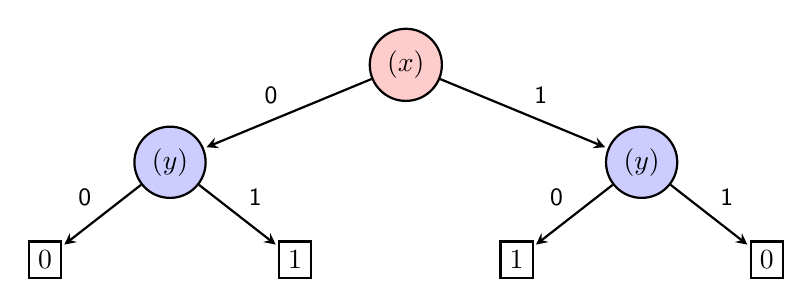
\begin{tikzpicture}[->,>=stealth,shorten >=1pt,auto,node distance=1.75cm, thick,main node/.style={scale=0.9,circle,draw,font=\sffamily\normalsize}]

            \node[circle, draw] (1)[fill=red!20] {$\xor(x)$};

            \node[circle, draw] (2) [below left of=1, xshift=-50, fill=blue!20]{$\xor(y)$};
            \node[circle, draw] (3) [below right of=1, xshift=50, fill=blue!20]{$\xor(y)$};

            \node[rectangle, draw] (4) [below left of=2, xshift=-10]{$0$};
            \node[rectangle, draw] (5) [below right of=2, xshift=10]{$1$};
            \node[rectangle, draw] (6) [below left of=3, xshift=-10]{$1$};
            \node[rectangle, draw] (7) [below right of=3, xshift=10]{$0$};

            \path[every node/.style={font=\sffamily\small}]
                (1) edge [swap] node{0} (2)
                (1) edge node{1} (3)
                (2) edge [swap] node{0} (4)
                (2) edge node{1} (5)
                (3) edge [swap] node{0} (6)
                (3) edge node{1} (7)
                ;
        \end{tikzpicture}

        \caption{Tree-like representation of the protocol computing $\mathrm{PARITY}$ on $2n$ bits.}
    \end{figure}

    Since the two parties have unlimited computational power, they can also evaluate functions that are \textbf{uncomputable} for Turing machines. For instance, a protocol could even compute the Halting problem. Let $H_n : \{0,1\}^{2n} \to \{0,1\}$ be the function that outputs 1 if the input is a string $1^n\abk{M}$ such that $M$ is a Turing machine that halts on $1^n$, and 0 otherwise. This function can be computed by the following protocol:
    
    \begin{enumerate}
        \item Since the first $n$ bits are Alice's input, they check if their input $x = 1^n$. They send 1 to Bob if the check succeeds and 0 otherwise.
        \item If the received bit is 0, Bob outputs 0. Otherwise, They check if $y = \abk{M}$ and if $M(1^n)$ halts. If both conditions are true, Bob outputs 1. Otherwise, they output 0.  
    \end{enumerate}

    Clearly, the Halting problem can be solved by computing the length of the input and then solving $H_n$. This concludes that, just like non-uniform circuits, protocols are \textit{incomparable} with Turing machines.


    \section{Fooling sets}

    As we did for circuits and decision trees, we will discuss methods for proving lower bounds on protocols. In particular, we will show various methods focus using the \textit{equality function} as an example.
    \[\mathrm{EQ}(x,y) = \soe{ll}{
        1 & \text{if } x = y \\
        0 & \text{otherwise} \\
    }\]

    In particular, we will show that $CC(\mathrm{EQ}) \geq n$. The fist technique is based on a an idea called \textbf{fooling set}. For any communication protocol and any function, suppose $x, x'$ are any two different $n$-bit strings such that the \textit{communication pattern} -- the sequence of bits transmitted -- is the same on the input pairs $(x, x)$ and $(x',x')$. Then, we claim that the players' final answer must be the same on all four input-pairs $(x, x), (x, x'), (x', x), (x', x')$, which can easily be shown by induction.

    To show that $CC(\mathrm{EQ}) \geq n$, we assume by way of contradiction that there exists a protocol whose complexity is at most $n - 1$, which can generate at most $2^{n-1}$ possible communication patterns. Since there are $2^n$ choices for input pairs of the form $(x, x)$, by the pigeonhole principle there must exists two distinct pairs $(x, x)$ and $(x', x')$ who share the same communication pattern. Thus, all the input pairs $(x, x), (x, x'), (x', x), (x', x')$ must return the same output. However, this implies that $1 = \mathrm{EQ}(x, x) = \mathrm{EQ}(x,x') = 0$, which is absurd, concluding that such protocol cannot exist.

    The argument that we have just shown can be generalized to every Boolean function through the concept of \textit{fooling sets}, a set of input combinations that \curlyquotes{fools} any invalid protocol into giving an a wrong answer by collision of possible communication patterns.

    \begin{frameddefn}{Fooling set}
        Given a function $f : \{0, 1\}^{2n} \to \{0, 1\}$, a \textbf{fooling set} of $f$ is a subset $S \subseteq \{0, 1\}^{2n}$ for which there is a value $b \in \{0, 1\}$ such that:
        \begin{enumerate}
            \item For every $(x,y) \in S$ it holds that $f(x,y) = b$
            \item For every distinct pair $(x,y), (x',y') \in S$ it holds that $f(x,y') \neq b$ or $f(x',y) \neq b$.
        \end{enumerate}
    \end{frameddefn}

    \begin{framedthm}{The fooling set method}
        Given a function $f : \{0, 1\}^{2n} \to \{0, 1\}$, for any fooling set $S$ of $f$ it holds that $CC(f) \geq \log \abs{S}$.
    \end{framedthm}

    \begin{proof}
        Let $\abs{S} = k$. By way of contradiction, suppose that there is a protocol $\Pi$ of depth less than $\log k$ that computes $f$. This protocol must induce less than $2^{\log k} = k$ communication patterns. Hence, at least two pairs $(x,y), (x',y') \in S$ will collide into the same communication pattern, meaning that $(x, y), (x, y'), (x', x), (x', y')$ must all return the same output, contradicting the very definition of $S$. This concludes that $\Pi$ must have depth at least $\log k$.
    \end{proof}

    The set $S = \{(x,y) \in \{0,1\}^{2n} \mid x = y\}$ is clearly a fooling set for $\mathrm{EQ}$ of size $2^n$, hence $CC(\mathrm{EQ}) \geq n$. Finding a fooling set for $\mathrm{EQ}$ that has size $2^{n+1}$ is no easy task, meaning that this method is not sufficient to give an exact value for $\mathrm{EQ}$.
    
    To give another example, consider the \textit{disjointness function}. Let $x, y \in \{0,1\}^n$ be two indicator vectors each representing a subset $A_x \subseteq \{1, 2, \ldots , n\}$, where $x_i = 1$ if and only if $i \in A_x$. The functions $\mathrm{DISJ}$ is defined as follows.
    \[\mathrm{Disj}(x,y) = \soe{ll}{
        1 & \text{if } A_x \cap A_y = \varnothing\\
        0 & \text{otherwise} \\
    }\]
    
    It's easy to see that the set $S = \{(x, \overline{x}) \mid A_x \subseteq \{1,\ldots, n\}\}$ is a fooling set of size $2^n$, hence $CC(\mathrm{DISJ}) \geq n$. Again, a fooling set of size $2^{n+1}$ cannot be easily found. In fact, in this case the set $S$ is the biggest fooling set that we can find.

    \section{Rectangles and tilings}

    The second method that we will discuss is the \textbf{tiling method}, which takes a more global view of the function $f$. Let $M_f$ denote the matrix of $f$, which is a $2^n \times 2^n$ matrix where each entry $m_{x,y}$ is the value $f(x,y)$.

    \begin{figure}[H]
        \centering
        \includegraphics[width=\textwidth]{images/function_matrix.pdf}
        \caption{Matrices of the equality and disjointess functions on 3 bits. White entries correspond to the output value 0, while black entries correspond to the output value 1.}
    \end{figure}

    The matrix representation of a function allows us to consider inputs in terms of \textit{combinatorial rectangles}. These rectangles are the building blocks of communication protocols.

    \begin{frameddefn}{Combinatorial rectangle}
        Given a function $f : \{0,1\}^{2n} \to \{0,1\}$, a \textbf{combinatorial rectangle} is subset of combinations of inputs for $f$. Formally, given two sets $A \subseteq \{0,1\}^n$ and $B \subseteq \{0,1\}^n$, the product $A \times B$ is a combinatorial rectangle.

        A rectangle $A \times B$ is said to be \textbf{monochromatic on $f$} when for all the pairs in the rectangle the function assumes the same value, i.e. $(x,y), (x',y') \in A \times B$ it holds that $f(x,y) = f(x',y')$.
    \end{frameddefn}

    We notice that, by definition, rectangles can also be defined on columns and rows that aren't necessarily adjacent to each other. For instance, the subset $\{000, 001, 010\} \times \{011, 101, 111\}$ is a rectangle. In other words, a rectangle can be viewed as a submatrix of $M_f$. Moreover, this rectangle is also monochromatic since each entry of the submatrix assumes the same value. Together with its graphical intuition, the name \curlyquotes{rectangle} also comes from the following combinatorial property.
    
    \begin{framedprop}[label=rectangles]{}
        The set $R \subseteq X \times Y$ is a rectangle if and only if whenever $(x,y), (x',y') \in R$ then $(x',y), (x,y') \in R$.
    \end{framedprop}

    Rectangles are a fundamental tool to understand how protocols compute. For instance, consider the tree-like representation of a protocol. If the root node is owned by Alice, $M_f$ gets \textbf{partitioned} into two rectangles $A_0 \times \{0, 1\}^n$ and $A_1 \times \{0, 1\}^n$, where $A_b \subseteq \{0,1\}^n$ is the subset of the input for which the Alice communicates the bit $b$. Clearly the sets $A_0$ and $A_1$ form a partition of $\{0, 1\}^n$. After the second bit is sent, each of the two rectangles above is further partitioned into two smaller rectangles. 

    \begin{figure}[H]
        \centering
        \includegraphics[scale=0.8]{images/rectangles.pdf}
        \caption{The 16 monochromatic rectangles of the equality function on 3 bits induced by the protocol where Alice sends all of her bits and then Bob computes the function.}
    \end{figure}

    If the total number of bits communicated is $k$ then the matrix gets partitioned into at most $2^k$ rectangles. Moreover, each of the rectangles induced by the protocol will be monochromatic. In other words, the set of all communication patterns induced by a protocol must lead to a partition of the matrix into monochromatic rectangles. Such partitions are called \textit{tilings}. \textcite{tiling_cc} used these partitions to give general strong lower and upper bounds on the communication complexity of Boolean functions.

    \begin{frameddefn}{Monochromatic tiling}
        Given a function $f : \{0,1\}^{2n} \to \{0,1\}$, a \textbf{monochromatic tiling} of $M_f$ is a partition of $M_f$ into disjoint monochromatic rectangles. We denote by $\chi(f)$ the minimum number of rectangles in any monochromatic tiling of $M_f$. 
    \end{frameddefn}

    By the previous observation, we know that any protocol that computes a Boolean function $f$ can induce a tiling with at most $2^{CC(f)}$ rectangles, hence $\log \chi(f) \leq CC(f)$. Hence, by finding lower bounds on the minimum monochromatic tiling, we can easily get lower bounds on communication complexity.

    For instance, consider again the $\mathrm{EQ}$ function discussed in the previous section. We'll now show that $CC(\mathrm{EQ})$ is exactly equal to $n+1$. First, we notice that if $R$ is a 1-monochromatic rectangle then $\abs{R} = 1$, meaning that only one pair of inputs lies inside that rectangle -- this can easily be seen in the matrix $M_{\mathrm{EQ}}$, but we're going to prove it for completeness.
    
    By way of contradiction, suppose that $\abs{R} > 1$, meaning that there are at least two distinct pairs $(x,y), (x',y') \in R$, hence either $x \neq x'$ or $y \neq y'$. Due to \Cref{rectangles}, we know that since $(x,y), (x',y') \in R$ we must also have that $(x',y), (x,y') \in R$. However, by definition of $\mathrm{EQ}$, this implies that $x = y = y' = x'$, which is a contradiction, concluding that $R = 1$ is the only option.

    Since $\mathrm{EQ}$ has $2^n$ combinations of inputs for which $\mathrm{EQ}(x,y) = 1$, any monochromatic tiling of $M_{\mathrm{EQ}}$ must have at least $2^n$ 1-monochromatic rectangles. Additionally, since there is at least one input pair for which $\mathrm{EQ}(x',y') = 0$, we will also require one additional 0-monochromatic rectangle for this pair. This concludes that any monochromatic tiling of $M_{\mathrm{EQ}}$ requires at least $2^n+1$ rectangles, which concludes that $n < \log \chi(f) \leq CC(\mathrm{EQ})$ and thus that $CC(\mathrm{EQ}) = n+1$.

    Like in the previous section, this reasoning can be generalized to \textit{fooling sets}: if $(x, y)$ and $(x', y')$ are two distrinct pairs of the fooling set then they cannot be in the same monochromatic rectangle since not all of $(x, y), (x, y'), (x', y), (x', y')$ can give the same output value. This means that each entry in the fooling set must be covered by a different rectangle, while at least another additional rectangle is required by the other color. 

    \begin{framedprop}{}
        Given a function $f : \{0,1\}^{2n} \to \{0,1\}$, for any fooling set $S$ it holds that 
        \[\chi(f) > \abs{S}\]
    \end{framedprop}
    
    Tilings are also useful upper bound tools. To prove this, we have to first define the concept of intersection between rectangles. We say that two rectangles $A \times B$ and $A' \times B'$ \textit{intersect horizontally} if $A \cap A' \neq \varnothing$, while they \textit{intersect vertically} if $B \cap B' \neq \varnothing$. By definition, two rectangles intersect both horizontally and vertically if and only if they \textbf{overlap}, meaning that they aren't disjoint: if $x \in A \cap A'$ and $y \in B \cap B'$ then $(x,y) \in A \times B$ and $(x,y) \in A' \times B'$, while if $A \cap A' = \varnothing$ and $B \cap B' = \varnothing$ then $A \times B \cap A' \times B' = \varnothing$.

    \begin{figure}[H]
        \centering
        \includegraphics[scale=0.7]{images/rect_int.pdf}

        \caption{The red rectangle horizontally intersects the blue rectangle and vertically intersects the green rectangle. The yellow rectangle intersects the red rectangle both horizontally and vertically.}
    \end{figure}

    Since all the rectangles of a tiling are pairwise disjoint, any rectangle from our collection cannot intersect every other rectangle in both ways. This suggests
    an approach to reduce the space of potential rectangles that could cover an input $(x, y)$.

    \begin{framedlem}{}
        Given a function $f : \{0,1\}^{2n} \to \{0,1\}$, if there is a monochromatic tiling of $M_f$ with $2^k$ rectangles then $CC(f) \leq k^2+1$
    \end{framedlem}

    \begin{proof}
        Let $\mathcal{R}$ be monochromatic tiling of $M_f$ with $2^k$ rectangles. We want to construct a protocol that for any input $(x,y)$ finds the unique rectangle $R_{x,y}$ containing it.

        We say that a rectangle $R \in \mathcal{R}$, where $R = A \times B$, is \textit{horizontally good} for an input $(x,y)$ if $x \in A$ and $R$ horizontally intersects at most $\frac{\abs{\mathcal{R}}}{2}$ rectangles in $\mathcal{R}$. Likewise, we say that $R$ is \textit{vertically good} for an input $(x,y)$ if $x \in B$ and $R$ vertically intersects at most $\frac{\abs{\mathcal{R}}}{2}$ rectangles in $\mathcal{R}$.

        \textbf{Claim:} Initially, the rectangle $R_{x,y}$ is either horizontally good or vertically good.

        \begin{proof}[Proof of the claim.]
            Since $\mathcal{R}$ is a partition, all the rectangles of our collection cannot intersect every other rectangle on both ways at the same time. Hence, either at most half of the rectangles in $\mathcal{R}$ intersect $R_{x,y}$ horizontally or at most half of them intersect $R_{x,y}$ vertically.
        \end{proof}
        
        Assuming all the rectangles are identified by a number ($\log 2^k = k$ bits suffice for the ID of a single rectangle), the protocol proceeds as follows. If there is a horizontally good rectangle $R_H$ in $\mathcal{R}$ that contains $x$ then Alice announces the ID of such rectangle. Otherwise, if there is a vertically good rectangle $R_V$ in $\mathcal{R}$ that contains $y$ then Bob announces the ID of such rectangle. Each time a rectangle is announced, the two players discard every single rectangle that doesn't intersect it in the designed direction: if Alice is the announcer, they discard all the rectangles that don't horizontally intersect it, otherwise they discard the ones that don't intersect it vertically. The process is then repeated using $\mathcal{R}'$, the set containing the non-discarded rectangles. 
        
        After each round of the procotol, $R_{x,y}$ will always be good in one of the two directions, meaning that there always is at least one good rectangle satisfying the selection process. We also observe that the selected good rectangle always intersects $R_{x,y}$ in the designed direction, hence $R_{x,y}$ will never get discarded. When only one rectangle remains, this rectangle must be $R_{x,y}$. After finding $R_{x,y}$, the last player sends a final output bit describing the color of $R_{x,y}$. Since each announcement leads to at least half of the rectangles in $\mathcal{R}$ being discarded, $\mathcal{R}$ can survive at most $k$ such discards, meaning that the communication complexity of the protocol is at most $k^2+1$
    \end{proof}

    \begin{framedthm}[label=tiling]{The tiling method}
        Given a function $f : \{0,1\}^{2n} \to \{0,1\}$, it holds that:
        \[\log \chi(f) \leq CC(f) \leq 1+\log^2 \chi(f)\]
    \end{framedthm}

    \section{The rank method and the log rank conjecture}

    The use of matrices as representations of functions opens the doors to the use of linear algebra in order to study the complexity of functions. In particular, the \textit{rank} of $M_f$ intrudices an algebraic method to lower bound $\chi(f)$ -- hence the communication complexity of $f$. We recall that the rank of a square matrix, written as $\mathrm{rk}(M)$, is the size of the largest subset of rows (or columns) that are linearly independent from each other. The following lemma, gives an equivalent characterization of the rank that is more practical for our case.

    \begin{framedlem}{Rank of a matrix}
        Given an $n \times n$ matrix $M$ over the field $\F$, $\mathrm{rk}(M)$ is the minimum value of $r$ such that $M$ can be expressed as $M = \sum_{i = 1}^r B_i$, where $B_1, \ldots, B_r$ are $n \times n$ matrices of rank 1,
    \end{framedlem}

    We notice that $0, 1$ are elements of every field, so we can compute the rank of a binary matrix over any field we like. Sometimes, the choice of the field can be crucial. Since it suffices, we will use the field $\R$ to make things easier. It's easy to see that every monochromatic rectangle of $M_f$ is nothing more than a square submatrix of $M_f$ -- also called a \textit{minor} -- filled with either all 0s or all 1s. This easily gives us the following lower bound.

    \begin{framedthm}{The rank method}
        Given a function $f : \{0,1\}^{2n} \to \{0,1\}$, over the field $\F_2$ it holds that:
        \[\chi(f) \geq \mathrm{rk}(M_f)\]
    \end{framedthm}

    For instance, since $M_{\mathrm{EQ}}$ is nothing more than the identity matrix $I_{2^n}$, it's rank is clearly $2^n$, giving us another way to prove that $CC(\mathrm{EQ}) \geq n$. However, we already shown that $CC(\mathrm{EQ}) = 1$ can be proven through the tiling method.

    The tiling argument is still the strongest lower bound technique known for communication complexity, since the fooling set and rank methods imply a lower bound on $\chi(f)$, meaning that they can never prove better lower bounds than the tiling argument. As shown in \Cref{tiling} -- up to a squared factor -- $\log \chi(f)$ strictly characterizes the communication complexity of any function $f$.
    
    Moreover, the rank and fooling set methods are incomparable: each method can be stronger than the other for some functions. However, if we ignore constant factors, the rank method is always at least as strong as the fooling set method. We also know functions for which a polynomial gap exists between $\log \chi(f)$ and $\log \mathrm{rk}(M_f)$.

    This gap has moved computer scientists to conjecture that the rank of $M_f$ may be sufficient to polynomially characterize the communication complexity of a function, i.e. that $CC(f)$ is upper bounded by $\log^k \mathrm{rk}(M_f)$ for some constant $k \in \N$. This is known as the \textbf{log rank conjecture}, first proposed by \textcite{log_rank}, and it's one of the most important questions in complexity theory: if such conjecture were to be true, the rank method could replace the tiling method since computing the rank of a matrix is an easy task that has been deeply studied by linear algebra, while computing optimal tilings is a tedious task.

    Currently, the best known upper bounds for such conjecture are $O(\sqrt{\mathrm{rk}(M_f)} \log \mathrm{rk}(M_f))$, proved by \textcite{lovett}, which was very recently improved by \textcite{sudakov} to $O(\sqrt{\mathrm{rk}(M_f)})$.

    \newpage

    \section{Protocol balancing}

    We have discussed how the tree-like representation of protocols is more convenient. Up untill now, this fact was only justified by the similarities between this representation and decision trees, giving us a more intuitive way to work with protocols. However, it turns out that protocols are actually fundamentally different from decision trees. In particular, this difference lies in the possibility of protocols to be \textbf{balanced}: if a protocol has relatively few vertices but a large depth -- meaning that most of the paths have very few vertices -- we can always transform the protocol into an equivalent protocol that approximately preserves the size of the tree while also significantly reducing the depth of the tree.

    To prove this result, we use a well-known result in binary trees called the $\frac{1}{3},\frac{2}{3}$ lemma.

    \begin{framedlem}[label=13_23_lemma]{$\frac{1}{2},\frac{2}{3}$ lemma}
        Given a binary tree $T$ with $s > 1$ nodes, there is a vertex $v$ such that the subtree $T_v$ rooted at $v$ contains $s'$ nodes, where $\frac{1}{3} s \leq s' \leq \frac{2}{3} s$
    \end{framedlem}

    \begin{proof}
        Consider the sequence of vertices $v_1, v_2 , \ldots, v_k$ defined as follows. The vertex $v_1$ is the root of $T$, while $v_k$ is a leaf of $T$. For each $i > 1$, the vertex $v_{i+1}$ is the child of $v_i$ with the biggest subtree $T_{v_{i+1}}$ -- in other words, if $v_i$ has two childs $x, y$ and $T_x$ has more nodes than $T_y$ then $v_{i+1} = x$.
        
        Given $i > 0$, let $s_i$ denote the number of nodes in $T_{v_i}$. Since $T$ is a binary tree, we have that $\frac{1}{2}s_i \leq s_{i+1} \leq s_{i} - 2$. Since $s_1 = s$ and $s_k = 1$, we know that $s_1, \ldots, s_k$ is a decreasing sequence. Hence, there must be some $i$ for which $\frac{1}{3} s \leq s_i \leq \frac{2}{3} s$.

        \textit{Note:} the original proof of these bounds is more detailed.
    \end{proof}

    \begin{figure}[H]
        \centering
        \includegraphics[scale=0.55]{images/13_23_lemma.pdf}

        \caption{The subtree whose root is the red node respects the $\frac{1}{2},\frac{2}{3}$ lemma}
    \end{figure}

    \begin{framedthm}{Protocol balancing}
        Given a protocol $\Pi$ of size $s$ that computes a function $f$, there is a protocol $\Pi'$ that also computes $f$ and has depth at most $2 \ceil{\log_{\frac{3}{2}} s}$.  
    \end{framedthm}

    \begin{proof}
        We'll recursively use the $\frac{1}{2},\frac{2}{3}$ lemma to discard communication patterns. For each node $v \in V(\Pi)$, let $X_v$ be the set of all the inputs $x$ of Alice for which there is an input $y$ of Bob such that $\Pi(x,y)$ passes through $v$. The set $Y_v$ follows the same definition, with the role of the two players reversed. Let $R_v = X_v \times Y_v$. We notice that $R_v$ is clearly a rectangle, but not necessarily a monochromatic one.

        Let $u \in V(\Pi)$ be the node that satisfies the lemma's condition. For any input $(x,y)$, Alice sends 1 to Bob if and only if $x \in X_{u}$ and Bob responds analogously with 1 if and only if $y \in Y_{u}$. If both bits sent are 1, Alice and Bob repeat this process on the subtree $\Pi_{u}$. Otherwise, they repeat this procedure on the subtree $\Pi - \Pi_u$.

        The recursive calls of these procedures define a new protocol $\Pi'$ -- in other words, $\Pi'$ computes the balanced simulation of $\Pi(x,y)$ for each input $(x,y)$. After each recursive application, the number of nodes in the tree is reduced by at most $\frac{2}{3}$. Hence, the process can be applied at most $\ceil{\log_{\frac{3}{2}} s}$ times, for a total of at most $2\ceil{\log_{\frac{3}{2}} s}$ communicated bits.
    \end{proof}

    We notice that the size of the new protocol can be at most $2^{2 \ceil{\log_\frac{3}{2} s}} \leq 4 s^2$, meaning that it may have more nodes than the original protocol. Moreover, this also implies that this balancing process cannot be applied multiple times to get an even lower depth -- after all, the final tree is already balanced after one application.

    \section{Randomized protocols}

    As we did for decision trees, we show how randomness can be used to give communication protocols that are far more efficient than the best possible deterministic protocols for many problems. Randomness can appear in several ways in communication protocols. In particular, we'll reuse lots of concepts already seen in \textit{interactive proofs}: Alice and Bob may use public or private coins, but we'll also allow their inputs to be random -- if needed.
    
    We say that a protocol uses \textbf{public coins} if both parties have access to a common shared random string. We usually denote this shared string as $R$. We say that the protocol uses private coins if each party privately samples an independent random string, denoted as $R_A$ and $R_B$. In other words, we have four potential sources of randomness - $R, R_A , R_B$ and the input $(x,y)$. These four random variables are always assumed to be independent.
    
    We'll also borrow the definition of random protocol from the alternative definition of decision trees that we discussed: a randomized protocol for a function $f$ is simply a \textbf{distribution} over the deterministic protocols that compute $f$.
    
    For example, consider again the equality function. We showed that the deterministic communication complexity of $\mathrm{EQ}$ is exactly $n+1$. Through randomness, we can achieve some better results. In particular, we can consider a trivial public coin protocol based on \textbf{hashing}. The public coins $R$ are used to define a hashing function $h : \{0,1\}^n \to \{0,1\}^k$. Then, Alice sends $h(x)$ to Bob, who then computes $h(y)$. If Bob finds that $h(y) = h(x)$, he'll assume that $x = y$ and return 1 and 0 otherwise. The number of bits communicated is always $k+1$ and the probability of making an error is at most $\frac{1}{2^k}$. The length of this protocol is clearly short, but it requires $k2^n$ shared random coins to define $h$.

    We can reduce the number of random bits used if we use an \textbf{error-correcting code}, i.e. a function $C : \{0, 1\}^n \to [2^k]^m$ such that if $x \neq y$ then $C(x)$ and $C(y)$ match in only $\frac{2^{\Omega(k)}}{m}$ coordinates. It can be proven that if $m$ is set to $10n$ then, for any $k$, most of the functions that respect these properties will be error-correcting codes.
    
    Given an error-correcting code $C$, Alice can pick a random coordinate of $C(x)$ and send it to Bob, who can then check whether this coordinate is matches $C(y)$ or not. This takes $\log_{10} m + \log k = O(\log n + k)$ bits of communication, while the probability of making an error is at most $\frac{1}{2^{\Omega(k)}}$. In this protocol, the parties do not require a shared random string because the choice of $C$ is made once and for all when the protocol is constructed, and before the inputs are seen.

    As for random decision trees, there are two ways to measure the probability that a randomized protocol makes an error: the \textbf{worst-case} error and the \textbf{average-case} error.
    
    We say that a randomized protocol has error $\varepsilon$ in the worst-case if for every input, the probability that the protocol makes an error is at most $\varepsilon$. In other words, for all input $(x,y) \in \{0,1\}^{2n}$ we have that:
    \[\Pr_{R, R_A, R_B} [\Pi_{R, R_A, R_B (x,y)} \text{ is wrong}] \leq \varepsilon\]
    
    Given a distribution on inputs $D$, we say that a protocol has error $\delta$ with respect to $D$ if the probability that the protocol makes an error is at most $\delta$ when the inputs are sampled from $D$. In other words, we have that:
    \[\Pr_{R, R_A, R_B, (x,y) \in D} [\Pi_{R, R_A, R_B (x,y)} \text{ is wrong}] \leq \delta\]

    In both cases, the depth of a random protocol is defined to be the maximum
    depth of all of the deterministic protocol trees that the protocol may
    generate. But why are these two definition equivalent? A good eye may have recognized that this is nothing more than the same concept as randomized complexity and distributional complexity in the context of decision trees. In fact, through \textbf{Yao's priciple} we can easily show that the \textit{worst-case randomized communication complexity} of
    a function $f$ with error at most $\varepsilon$ is equal to the maximum, over all distributions $D$ on inputs, of the \textit{average-case communication complexity}
    of $f$ with error at most $\varepsilon$ with respect to $D$. 

    \chapter{Proof complexity}

    \section{Propositional proof systems}
    
    \textbf{Proof complexity} is the branch of complexity theory that studies the complexity measures needed for a propositional formula to be proved by propositional proof systems, that being any system of rules that can prove the truthfulness of a propositional formula. But why are we interested in proving or refusing propositional formulas? We discussed how the $\mathrm{TAUT}$ problem is \textsf{coNP}-Complete. Researchers gave birth to the field of proof complexity in order to find an algorithm that could verify in polynomial time if a formula is a tautology or not, i.e. if $\mathrm{TAUT} \in \mathsf{NP}$, proving that $\mathsf{NP} = \mathsf{coNP}$.

    The easiest way to find such algorithm is through the use of \textbf{proof systems}. Proof systems can be viewed as an algorithm that manipulates propositional formulas, producing new ones until the proof is completed. Given the encoding $\Pi$ of a proof of $F$ in a proof system $P$, a verifier can follow the rules of $S$ to prove that $F$ is indeed a tautology. In this case, $\Pi$ serves as a certificate for $F$ while $P$ defines how the verifier works. In 1979, \textcite{proof_system} defined the concept of \textbf{propositional proof system}, often called \textit{Cook-Reckhow proof systems}.

    \begin{frameddefn}{Propositional proof system}
        A \textbf{propositional proof system (PPS)} is a verifier $P$ such that
        \[F \in \mathrm{TAUT} \iff \exists \Pi \in \{0,1\}^* \; P(F,\Pi) = 1\]
        and that runs in polynomial time with respect to $\abs{F}+\abs{\Pi}$.
    \end{frameddefn}

    This definition clearly implies that any PPS is both \textit{sound} and \textit{complete}, making it a good tool of reasoning -- this doesn't break Gödel's incompleteness theorem due to these propositional systems not being powerful enough.

    At first glance, one could think that this definition implies that any such system proves that $\mathrm{TAUT} \in \mathsf{NP}$. However, we must also consider the length of such proofs: to be a \curlyquotes{standard} polynomial time verifier, the length of the certificates must be \textit{polynomially bounded} by the length of $F$. In other words, it must hold that $\abs{\Pi} = \abs{F}^{O(1)}$. When every tautology has a proof of size polynomially bounded by the size of the tautology itself, we say that it is a \textbf{polynomially bounded proof system}. 

    \begin{framedprop}{}
        There is a polynomially bounded proof system if and only if $\mathsf{NP} = \mathsf{coNP}$.
    \end{framedprop}

    We already discussed how researchers believe that $\mathsf{NP} \neq \mathsf{coNP}$ is the expected answer to the conjecture. Proving this statement through proof complexity is no easy task: we would have to prove that there is a particular formula $F$ that strictly requires an exponential length encoding for every discovered and undiscovered proof system.

    Does this mean that proof complexity is useless? To prove that $\mathsf{NP} \neq \mathsf{coNP}$, yes, it definitely is. In practice, it's still useful. For example, among the major challenges of proof complexity is showing that the \textbf{Frege system}, the usual propositional calculus that mathematicians and logicians use, does not admit polynomial-size proofs of all tautologies. Here the size of the proof is simply the number of symbols in it, i.e. the length of the corresponding certificate. Moreover, proof systems are used in \textbf{SAT Solvers}, programs that are currently used in industry in order to decide if a statement is true or false -- remember that potentially any statement can be encoded as a propositional formula.

    In particular, researchers are interested in the performance of proof systems for very basic combinatorial principles, such as the \textit{pigeonhole principle} or the \textit{handshaking lemma}. If a PPS requires proofs of exponential size for these basic principles, any problem that is built on them is untreatable by that very proof system. Moreover, it's important to notice that many advanced proof systems like the Frege systems are indeed powerful, but \textbf{not automatizable}, meaning that we cannot build a polynomial time verifier that simulates that proof system.

    Most proof systems are based on the concept of \textbf{refutation}, a \curlyquotes{proof} of the fact that a formula is \textit{unsatisfiable}. Even though they achieve the opposite of what we want, refutations can still be used as a proof: the formula $F$ is a tautology if and only if $\lnot F$ is unsatisfiable. In other words, most proof systems actually work on $\mathrm{UNSAT}$ instead of $\mathrm{TAUT}$. In particular, the proof systems that will be analyzed in the following sections are all based on refutations. Moreover, we'll assume to be always working with CNF formulas since $\mathrm{SAT}$ and $\mathrm{CNF\text{-}SAT}$ are both $\mathsf{NP}$-Complete.

    \newpage

    \section{Decision trees and DPLL algorithms}

    The first proof system that we'll analyze is based on decision trees. In particular, we'll be using a generalization of the concept of decision trees, where the output is a value from a set of outputs $O$, instead of a 0 or 1.

    Given a CNF formula $F = \bigwedge_{i = 1}^m C_i$ defined on $n$ variables, a \textbf{satisfiability decision tree} is a decision tree whose leaves are either one of the axioms of $F$, that being the clauses $C_1, \ldots, C_m$, that is falsified by the (partial) assignment dictated by the path or the value \curlyquotes{Sat}, which says that every clause of $F$ is satisfied by that assignment.

    \begin{figure}[H]
        \centering

        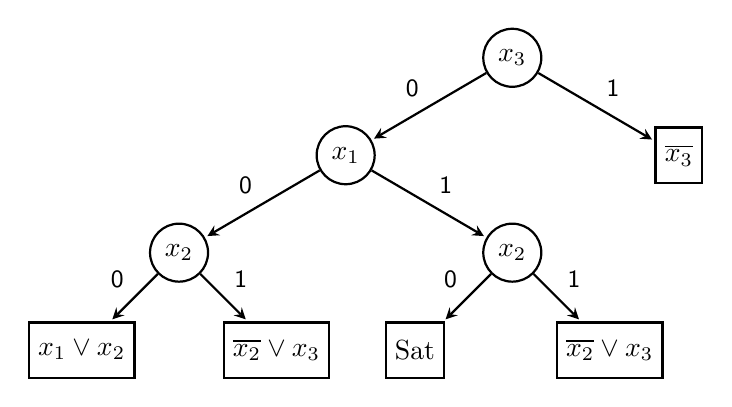
\begin{tikzpicture}[->,>=stealth,shorten >=1pt,auto,node distance=1.75cm, thick,main node/.style={scale=0.9,circle,draw,font=\sffamily\normalsize}]

            \node[circle, draw] (1)[] {$x_3$};

            \node[circle, draw] (2) [below left of=1, xshift=-25, ]{$x_1$};
            \node[rectangle, draw, minimum height=20] (3) [below right of=1, xshift=25 ]{$\overline{x_3}$};

            \node[circle, draw] (4) [below left of=2, xshift=-25]{$x_2$};
            \node[circle, draw] (5) [below right of=2, xshift=25]{$x_2$};

            \node[rectangle, draw, minimum height=20] (12) [below left of=4,]{$x_1 \lor x_2$};
            \node[rectangle, draw, minimum height=20] (13) [below right of=4,]{$\overline{x_2} \lor x_3$};
            \node[rectangle, draw, minimum height=20] (10) [below left of=5,]{$\mathrm{Sat}$};
            \node[rectangle, draw, minimum height=20] (11) [below right of=5,]{$\overline{x_2} \lor x_3$};

            \path[every node/.style={font=\sffamily\small}]
                (1) edge[swap, ]  node{0} (2)
                (1) edge node{1}(3)

                (2) edge[swap]  node{0} (4)
                (2) edge[]  node{1}(5)

                (4) edge[swap]  node{0} (12)
                (4) edge  node{1}(13)

                (5) edge[swap]  node{0} (10)
                (5) edge[]  node{1}(11)
                ;
        \end{tikzpicture}

        \caption{Decision tree for the formula $F = (x_1 \lor x_2) \land (\overline{x_2} \lor x_3) \land \overline{x_3}$.}
    \end{figure}

    Here, any decision tree without satisfying leaves is a \textit{refutation} for $F$. The decision tree proof system $(\mathsf{DTree})$ is both \textit{sound} and \textit{complete}: a formula $F$ is unsatisfiable if and only if it has a decision tree refutation. The complexity measure that will be of our interest in this proof system is the \textit{size} of the decision tree: by encoding the decision tree of size $s$ as a string, we get a witness of length $\Theta(s)$.

    \begin{figure}[H]
        \centering

        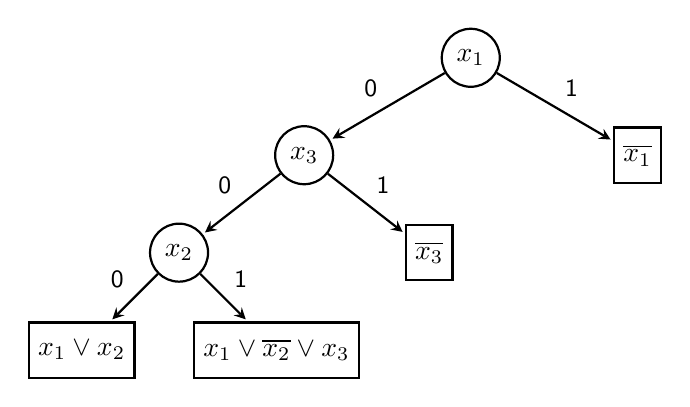
\begin{tikzpicture}[->,>=stealth,shorten >=1pt,auto,node distance=1.75cm, thick,main node/.style={scale=0.9,circle,draw,font=\sffamily\normalsize}]

            \node[circle, draw] (1)[] {$x_1$};

            \node[circle, draw] (2) [below left of=1, xshift=-25, ]{$x_3$};
            \node[rectangle, draw, minimum height=20] (3) [below right of=1, xshift=25 ]{$\overline{x_1}$};

            \node[circle, draw] (4) [below left of=2, xshift=-10]{$x_2$};
            \node[rectangle, draw, minimum height=20] (5) [below right of=2, xshift=10]{$\overline{x_3}$};

            \node[rectangle, draw, minimum height=20] (12) [below left of=4,]{$x_1 \lor x_2$};
            \node[rectangle, draw, minimum height=20] (13) [below right of=4,]{$x_1 \lor \overline{x_2} \lor x_3$};

            \path[every node/.style={font=\sffamily\small}]
                (1) edge[swap, ]  node{0} (2)
                (1) edge node{1}(3)

                (2) edge[swap]  node{0} (4)
                (2) edge[]  node{1}(5)

                (4) edge[swap]  node{0} (12)
                (4) edge  node{1}(13)
                ;
        \end{tikzpicture}

        \caption{Decision tree refutation for $F = \overline{x_1} \land (x_1 \lor x_2) \land (x_1 \lor \overline{x_2} \lor x_3) \land \overline{x_3}$.}
        \label{dt_ref}
    \end{figure}

    The decision tree proof system is highly related to a well-known SAT Solver algorithm, the  \textbf{Davis-Putnam-Logemann-Loveland (DPLL) algorithm}. This algorithm is capable of finding a satisfying (partial) assignment if and only if the given formula is satisfiable.

    \begin{framedalgo}{DPLL algorithm}
        Given an input CNF $F$, the following algorithm returns a satisfying (partial) assignment if and only if $F \in \mathrm{SAT}$:

        \begin{algorithmic}
            \Function{DPLL}{$F$}
                \If{$F = \top$ or $F = \bot$}
                \State \textbf{return} $\varnothing$
                \ElsIf{ there is a unit clause $C_i = \ell_j$}
                    \State \textbf{return} \textsf{DPLL($F_{\mid \ell_j = 1}$)}
                \Else
                    \State Pick $x_k \in \{x_1, \ldots, x_n\}$
                    \State Pick $b \in \{0,1\}$
                    \If{$F$ is satisfied by \textsf{DPLL($F_{\mid x_k = b}$)} $\cup \{x_i = b\}$}
                        \State \textbf{return} \textsf{DPLL($F_{\mid x_k = b}$)} $\cup \{x_k = b\}$
                    \ElsIf{$F$ is satisfied by \textsf{DPLL($F_{\mid x_k = 1-b}$)} $\cup \{x_k = 1-b\}$}
                        \State \textbf{return} \textsf{DPLL($F_{\mid x_k = 1-b}$)} $\cup \{x_k = 1-b\}$
                    \Else
                        \State \textbf{return} $\varnothing$
                    \EndIf
                \EndIf
            \EndFunction
        \end{algorithmic}
    \end{framedalgo}

    Here, the value $\top$ represents the \textbf{true clause}, the formula that is satisfied by every assignment, while $\bot$ represents the \textbf{false clause} (also called the \textit{empty clause}), is the formula that is falsified by every assignment. 
    
    The idea behind the DPLL algorithm is the following. If the formula contains a unit clause $C_i = \ell_j$ then $\ell_j$ must be set to 1 in order for $F$ to be satisfiable. Hence, the algorithm always gives priority to such unit clauses. This process is called \textbf{unit propagation}. If there is no unit clause, the algorithm picks a variable $x_k$ and a value $b$, testing if assigning $x_k = b$ can yield a satisfying assignment. To test this, the formula $F$ gets restricted on $x_k = b$. The restricted formula may or not  have unit clauses that can be propagated. The way the variable $x_k$ and the value $b$ are chosed depends on the type of DPLL algorithm used (e.g. the most frequent variable, the lowest variable, ...). These algorithms have now become a whole branch of theoretical computer science: under the right circumstances, some of them perform extremely well.
    
    For instance, consider the formula $F = x_1 \land (\overline{x_1} \lor x_2 \lor x_3) \land (x_2 \lor \overline{x_3})$. A DPLL algorithm may procede as follows. Initially, $\overline{x_1}$ is a unit clause, hence $x_1 = 1$ must be enforced. The formula gets restricted to $F_{\mid {x_1} = 1} = (x_2 \lor x_3) \land (x_2 \lor \overline{x_3})$. Since there are no unit clauses. The algorithm picks the variable $x_2$ and the value $b = 0$. We then have two ways to procede:
    \begin{itemize}
        \item We use the assignment $x_2 = 0$. The formula becomes $F_{\mid x_1 = 1, x_2 = 0} = x_3 \land \overline{x_3}$. Since $x_3$ is a unit clause, we propagate $x_3 = 1$. However, the formula now becomes $F_{\mid x_1 = 1, x_2 = 0, x_3 = 1} = \bot$. After traversing the recursive steps backwards, the final returned assignment is $\varnothing$.
        \newpage

        \item We use the assignment $x_2 = 1$. The formula now becomes $F_{\mid x_1 = 1, x_2 = 1, x_3 = 1} = \top$. After traversing the recursive steps backwards, the final returned partial assignment is $x_1 = 1, x_2 = 1, x_3 = *$.
    \end{itemize}

    The computation that we have just described can be viewed as nothing more than a decision tree. In particular, the depth of this decision tree is polynomially bounded (both upper and lower bounded) by the running time of the DPLL. This implies that if $F$ has a decision tree complexity lower bounded by $d$, the running time of the DPLL algorithm will be $d^{\Omega(1)}$.

    \begin{figure}[H]
        \centering

        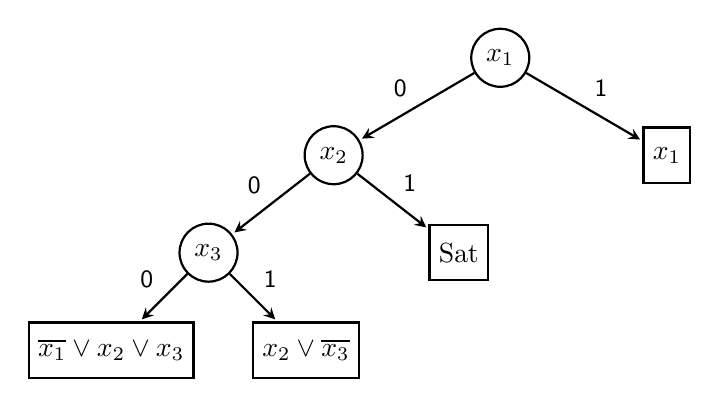
\begin{tikzpicture}[->,>=stealth,shorten >=1pt,auto,node distance=1.75cm, thick,main node/.style={scale=0.9,circle,draw,font=\sffamily\normalsize}]

            \node[circle, draw] (1)[] {$x_1$};

            \node[circle, draw] (2) [below left of=1, xshift=-25, ]{$x_2$};
            \node[rectangle, draw, minimum height=20] (3) [below right of=1, xshift=25 ]{$x_1$};

            \node[circle, draw] (4) [below left of=2, xshift=-10]{$x_3$};
            \node[rectangle, draw, minimum height=20] (5) [below right of=2, xshift=10]{$\mathrm{Sat}$};

            \node[rectangle, draw, minimum height=20] (12) [below left of=4,]{$\overline{x_1} \lor x_2 \lor x_3$};
            \node[rectangle, draw, minimum height=20] (13) [below right of=4,]{$x_2 \lor \overline{x_3}$};

            \path[every node/.style={font=\sffamily\small}]
                (1) edge[swap, ]  node{0} (2)
                (1) edge node{1}(3)

                (2) edge[swap]  node{0} (4)
                (2) edge[]  node{1}(5)

                (4) edge[swap]  node{0} (12)
                (4) edge  node{1}(13)
                ;
        \end{tikzpicture}

        \caption{Decision tree induced by the previous DPLL computation}
    \end{figure}

    This gives us reason to study the proof complexity of formulas in the context of the decision tree proof system. In this PPS, many formulas require an exponential size decision tree. This means that any DPLL algorithm based on unit propagation requires exponential runtime in the worst case.

    \section{Resolution}

    \textbf{Resolution} is one the most studied proof system, mainly for its semplicity. In fact, given a CNF $F$, this proof system is based on two simple rules:
    \begin{itemize}
        \item The \textbf{weakening rule}: if $C$ is a clause and $D$ is a clause then from $C$ we can derive $C \lor D$
        \[\frac{C}{C \lor D}\]
        The derived clause $C \lor D$ is called a \textit{weakening}
        \item The \textbf{resolution rule}: if $C \lor x_i$ and $\overline{x_i} \lor D$ are clauses then we can derive $C \lor D$ 
        \[\frac{C \lor x_i \quad \overline{x_i} \lor D}{C \lor D}\]
        The derived clause $C \lor D$ is called a \textit{resolvant}
    \end{itemize}

    The correctness of these two rules can be easily proven. For the weakening rule, every time $C$ is true the disjunction $C \lor D$ is also true. For the resolution rule, every time both $C \lor x_i$ and $\overline{x_i} \lor D$ are true, one of the two clauses must be satisfied by $C$ or $D$ since $x_i$ and $\overline{x_i}$ cannot both be true at the same time, concluding that $C \lor D$ must be true.

    The idea behind the \textbf{Resolution} ($\mathsf{Res}$) proof system is simple: if by repeatedly applying both rules we can derive the false clause $\bot$ from the \textbf{axioms} -- the initial clausees of $F$ -- then the formula is unsatisfiable. In fact, it can be easily shown by induction that a formula $F$ is unsatisfiable if and only if the false clause can be derived from its axioms.

    \begin{frameddefn}{Resolution refutation}
        Given an unsatisfiable CNF formula $F = \bigwedge_{i = 1}^m C_i$, a \textbf{resolution refutation} of $F$ is a sequence of clauses $D_1, \ldots, D_k$ such that $D_k = \bot$ and for each $i$ one of the following holds:
        \begin{itemize}
            \item $D_i$ is an axiom of $F$, i.e. $D_i = C_j$ for some $j$
            \item $D_i$ is the weakening of $D_j$, where $j < i$ 
            \item $D_i$ is the resolvant of $D_j$ and $D_h$, where $j,h < i$ 
        \end{itemize}
    \end{frameddefn}

    For instance, given the following unsatisfiable CNF formula
    \[(x_2 \lor x_3) \land (x_2 \lor \overline{x_3}) \land (x_1 \lor \overline{x_2} \lor x_3) \land (\overline{x_1} \lor \overline{x_2} \lor x_3) \land \overline{x_3}\]
    
    a resolution refutation for $F$ is given by:
    \[\begin{array}{lcl}
        D_1 :& \overline{x_3} & \text{Axiom} \\
        D_2 :& \overline{x_1} \lor \overline{x_2} \lor x_3 & \text{Axiom} \\
        D_3 :& x_1 \lor \overline{x_2} \lor x_3 & \text{Axiom} \\
        D_4 :& \overline{x_1} \lor \overline{x_2} & \text{Res. on $D_1, D_2$} \\
        D_5 :& x_1 \lor \overline{x_2} & \text{Res. on $D_1, D_3$} \\
        D_6 :& x_2 \lor x_3 & \text{Axiom} \\
        D_7 :& x_2 \lor \overline{x_3} & \text{Axiom} \\
        D_8 :& x_2 & \text{Res. on $D_6,D_7$} \\
        D_9 :& \overline{x_1} & \text{Res. on $D_4, D_8$} \\
        D_{10} :& x_1 & \text{Res. on $D_5, D_8$} \\
        D_{11} :& \bot & \text{Res. on $D_9, D_{10}$} \\
    \end{array}\]

    The \textit{length} of a resolution refutation is the number of clauses in the refutation, while the \textit{width} is the maximum number of literals that can be found in any of its clauses. For instance, the previous refutation has length 11 and width 3.

    To make things easier to read, each refutation can also be graphically represented by connecting clauses with lines, generating a DAG (Directed Acyclic Graph). Resolution refutations expressed in this form are also called dag-like refutations.

    \begin{figure}[H]
        \centering
        
        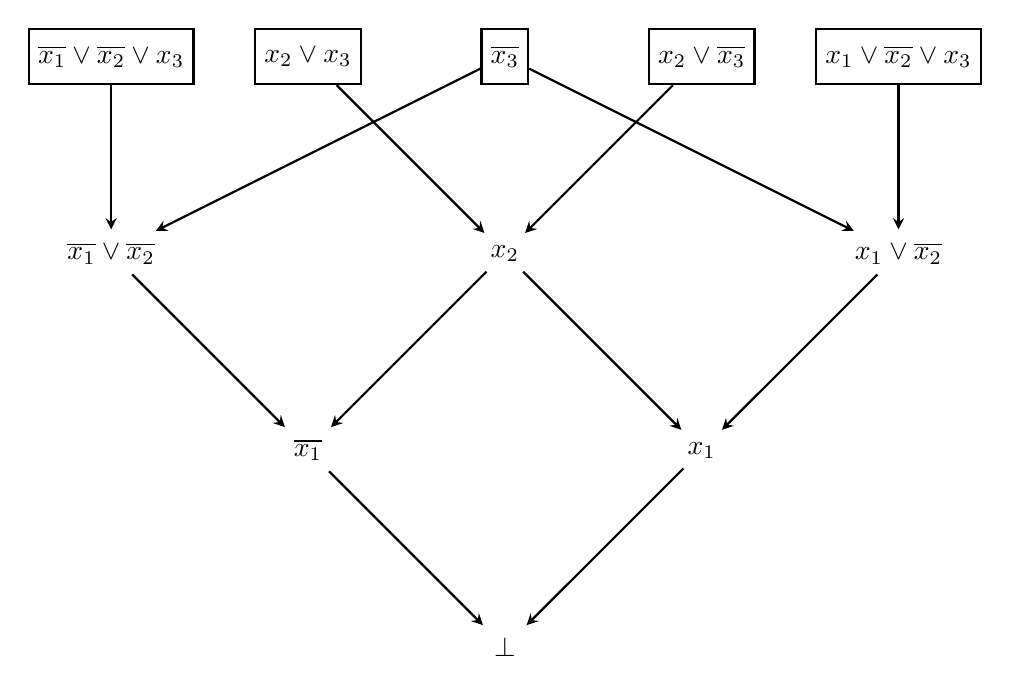
\begin{tikzpicture}[->,>=stealth,shorten >=1pt,auto,node distance=2.5cm, thick,main node/.style={scale=0.9,circle,draw,font=\sffamily\normalsize}]
            \node [rectangle, draw, minimum height=20](1) []{$\overline{x_1} \lor \overline{x_2} \lor x_3$};
            \node [rectangle, draw, minimum height=20](2) [right of=1]{$x_2 \lor x_3$};
            \node [rectangle, draw, minimum height=20](3) [right of=2]{$\overline{x_3}$};
            \node [rectangle, draw, minimum height=20](4) [right of=3]{$x_2 \lor \overline{x_3}$};
            \node [rectangle, draw, minimum height=20](5) [right of=4]{$x_1 \lor \overline{x_2} \lor x_3$};

            \node (6) [below of=1]{$\overline{x_1} \lor \overline{x_2}$};
            \node (x) [below of=2]{};
            \node (7) [below of=3]{$x_2$};
            \node (y) [below of=4]{};
            \node (8) [below of=5]{$x_1 \lor \overline{x_2}$};

            \node (9) [below of=x]{$\overline{x_1}$};
            \node (10) [below of=y]{$x_1$};
            \node (z) [below of=7]{};
            
            \node (11) [below of=z]{$\bot$};
        
            \path[every node/.style={font=\sffamily\small}]
                (1) edge (6)
                (2) edge (7)
                (3) edge (6)
                (3) edge (8)
                (4) edge (7)
                (5) edge (8)

                (6) edge (9)
                (7) edge (9)
                (7) edge (10)
                (8) edge (10)

                (9) edge (11)
                (10) edge (11)
                ;
        \end{tikzpicture}
        
        \caption{Dag-like representation of the previous refutation.}
    \end{figure}

    By definition, each clause $D_i$ can be used as premise for more than one rule application, both through weakening and resolution. When each $D_i$ of the proof is used \textbf{only once}, we say that it is a \textit{tree-like refutation} due to how the underlying dag becomes a tree. This restriction implies that if we want to use a clause multiple times then it must be derived again (or simply copied if it's an axiom). Clearly, this duplication process allows us to transform any dag-like refutation into a tree-like refutation, but this usually blows up the length of the proof exponentially.

    \begin{figure}[H]
        \centering
        
        \resizebox{1\hsize}{!}{
            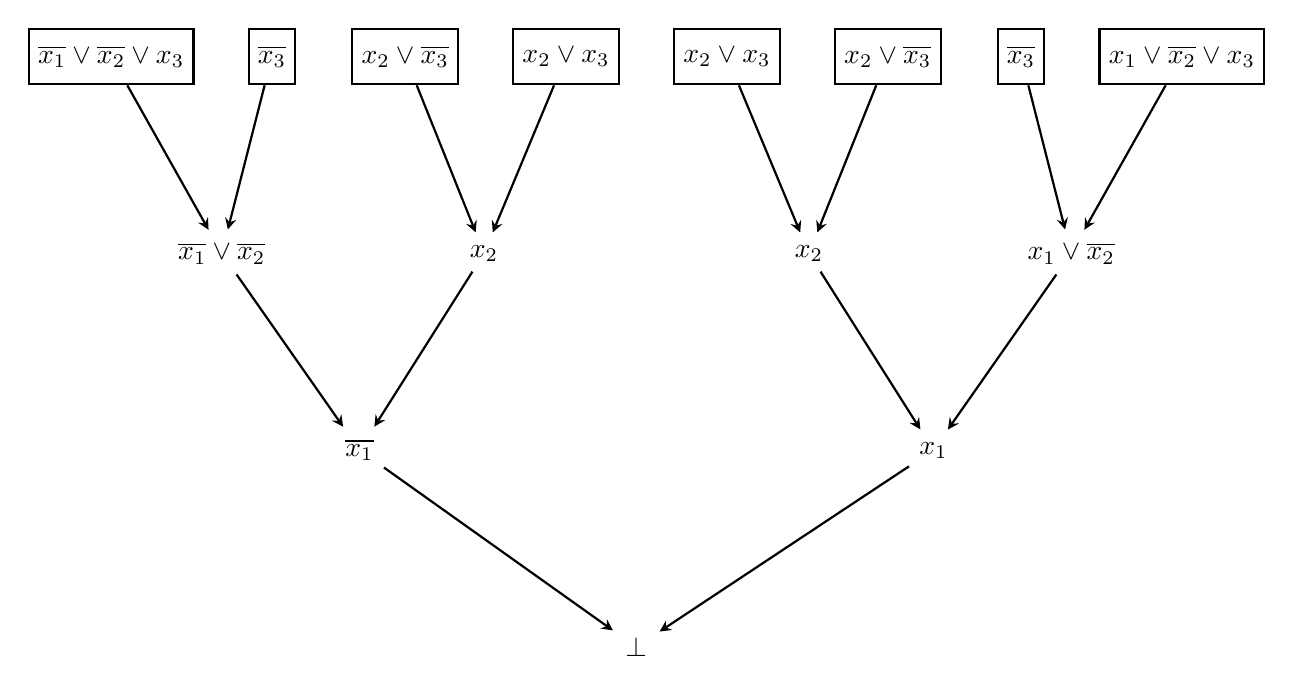
\begin{tikzpicture}[->,>=stealth,shorten >=1pt,auto,node distance=2.5cm, thick,main node/.style={scale=0.9,circle,draw,font=\sffamily\normalsize}]
                \node [rectangle, draw, minimum height=20](1) []{$\overline{x_1} \lor \overline{x_2} \lor x_3$};
                \node [rectangle, draw, minimum height=20](2) [right of=1, xshift=-13]{$\overline{x_3}$};
                \node [rectangle, draw, minimum height=20](3) [right of=2, xshift=-23]{$x_2 \lor \overline{x_3}$};
                \node [rectangle, draw, minimum height=20](4) [right of=3, xshift=-13]{$x_2 \lor x_3$};
                \node [rectangle, draw, minimum height=20](5) [right of=4, xshift=-13]{$x_2 \lor x_3$};
                \node [rectangle, draw, minimum height=20](6) [right of=5, xshift=-13]{$x_2 \lor \overline{x_3}$};
                \node [rectangle, draw, minimum height=20](7) [right of=6, xshift=-23]{$\overline{x_3}$};
                \node [rectangle, draw, minimum height=20](8) [right of=7, xshift=-13]{$x_1 \lor \overline{x_2} \lor x_3$}; 

                \node (9)[below of=1, xshift=40]{$\overline{x_1} \lor \overline{x_2}$};
                \node (10)[below of=3, xshift=28.5]{$x_2$};
                \node (11)[below of=6, xshift=-28.5]{$x_2$};
                \node (12)[below of=8, xshift=-40]{$x_1 \lor \overline{x_2}$};

                \node (13)[below of=10, xshift=-45]{$\overline{x_1}$};
                \node (14)[below of=11, xshift=45]{$x_1$};

                \node (15)[below of=13, xshift=100]{$\bot$};
            
                \path[every node/.style={font=\sffamily\small}]
                    (1) edge (9)
                    (2) edge (9)
                    (3) edge (10)
                    (4) edge (10)
                    (5) edge (11)
                    (6) edge (11)
                    (7) edge (12)
                    (8) edge (12)

                    (9) edge (13)
                    (10) edge (13)
                    (11) edge (14)
                    (12) edge (14)

                    (13) edge (15)
                    (14) edge (15)
                    ;
            \end{tikzpicture}
        }

        \caption{Tree-like refutation of the previous formula.}
        \label{treelike_res_proof}
    \end{figure}

    This subset of proofs defines a restricted proof system called \textbf{Tree-like Resolution} (\textsf{TreeRes}). In this context, we're interested in a new complexity parameter: the \textit{depth} of the refutation tree. The depth parameter is enough to give us an upper bound on the lenght of the refutation.

    We notice that in the two previous proofs we never used the weakening rule. In fact, it can be proven that any resolution refutation that uses both rules can be transformed into a resolution refutation that uses only the resolution rule. 

    \begin{framedthm}{No weakening resolution}
        Let $F$ be a CNF unsatisfiable formula. If $F$ has a resolution refutation that uses both rules then there is a resolution refutation that uses only the resolution rule. The new refutation may have lower size and depth.
    \end{framedthm}

    \begin{proof}
        Consider a resolution proof $D_1, \ldots, D_k$ for $F$ that uses both rules. We'll build a new refutation $Q_1, \ldots, Q_k$ for $F$ that never uses the weakening rule. Moreover, each $Q_i$ will be a subformula of $D_i$.

        For each $i \leq k$, we define $Q_i$ as follows:
        \begin{itemize}
            \item If $D_i$ is an axiom of $F$ then set $Q_i = D_i$
            \item If $D_i$ is a weakening of $D_j$ for some $j < i$ then set $Q_i = Q_j$
            \item If $D_i$ is a resolvant of $D_j = A \lor x_t$ and $D_h = \overline{x_t} \lor B$ then we have three cases:
            \begin{enumerate}
                \item If $x_t \notin Q_j$ then set $Q_i = Q_j$
                \item If $\overline{x_t} \notin Q_h$ then set $Q_i = Q_h$
                \item if $x_t \in Q_j$ and $\overline{x_t} \in Q_h$ then set $Q_i$ as the resolvant of $Q_j$ and $Q_h$ on $x_t$
            \end{enumerate}
        \end{itemize}

        The idea behind this construction is that any time we have previously used a weakening rule, we can postpone such weakening until we reach the first resolution step and then manipulate this step in order to make the weakening not needed anymore.
        
        The sequence of clauses $Q_1, \ldots, Q_k$ is by construction a refutation of $F$ since each $Q_i$ is a subformula of $D_i$, meaning that $Q_k$ is a subformula of the false clause $D_k = \bot$, which can only be true if $Q_k = \bot$. Finally, the clauses of $Q_1, \ldots, Q_k$ that are duplicates and aren't needed by subsequent clauses can be removed, obtaining a potentially shorter refutation.
    \end{proof}

    This result implies that the weakening rule is technically \textit{useless} in the resolution proof system since we could actually get a proof of lower size and depth -- in fact, sometimes this rule is directly omitted. We'll keep the weakening rule to make some of the following proofs easier.

    \newpage

    \section{Simulation between proof systems}

    One of the most interesting characteristics of proof systems is the ability to \textbf{simulate} each other. In particular, some proof system $P$ may be able to simulate a proof system $P'$, but the reverse may not hold. This allows us to define a \textbf{proof system hierarchy}. Some proof systems are clearly more powerful than others. For instance, the proof system based on the \textit{ZFC axioms} -- the commonly used axioms of set theory on which modern math is built -- is clearly more powerful than any proof system that we can define since that very system would be build though the ZFC axioms themselves, while resolution is not strong enough to simulate ZFC since resolution is complete and sound while ZFC cannot be due to Gödel's theorem.

    \begin{frameddefn}{Simulation between proof systems}
        Given two proof systems $P, P'$, we say that $P'$ \textbf{simulates} $P$ if for all unsatisfiable CNF formulas $F$ and for all proofs $\pi$ of $F$ in $P$ there is a proof $\pi'$ of $F$ in $P'$ obtainable through $\pi$. If it also holds that $\abs{\pi'} \leq \abs{\pi}^{O(1)}$, we say that $P'$ \textbf{p-simulates} $P$, written as $P' \leq_p P$. If two proof systems can p-simulate each other, we say that they are p-equivalent, written as $P \equiv_p P'$.
    \end{frameddefn}

    We notice that in the notation $P' \leq_p P$, the $\leq_p$ symbols references how $P'$ may have shorter proofs for a formula then $P$ since the proof obtained through the simulation may not be the shortest possible one. In other words, here the $\leq_p$ symbol compares the \textit{lengths of the proofs} of the two systems instead of comparing their hardness. When two proof systems are p-equivalent, their proofs have always almost the same size.
    
    We'll show that two of the proof systems that we have discussed -- decision trees and tree-like resolution -- are are p-equivalent. This equivalence comes in a natural way: any decision tree refutation can be \curlyquotes{rotated} into a tree-like resolution refutation and vice versa \cite{dt_tres}.
    
    \begin{framedlem}{$\mathsf{TreeRes}$ p-simulates $\mathsf{DTrees}$}
        Let $F$ be an unsatisfiable CNF formula. If $F$ has a decision tree refutation of size $s$ and depth $d$, there is a tree-like resolution refutation of length at most $2s$ and depth at most $d+1$.
    \end{framedlem}

    \begin{proof}
        
        Let $T$ be a decision tree refutation of size $s$ and depth $d$. The idea is to associate inductively a clause $C(v)$ to each node $v$ of $T$ in order to transform $T$ in a tree-like refutation of $F$. In particular, the partial assignment defined by the path from the root $r$ of $T$ to any node $v$ of $T$ will falsify the clause $C(v)$. 
        
        First, let $C(r) = \bot$, where $r$ is the root note. Since $\bot$ is falsified by every assignment, the hypothesis holds for this base case. Consider now a node generic node $v$ of $T$. By induction, assume that $v$ has already been associated with $C(v)$ and that the partial assignment given by the path from $r$ to $v$ falsifies $C(v)$.
        
        Let $u,w$ be the left and right children of $v$. Let $x_i$ be the variable queried by $v$. Since the answer $x_i = 0$ leads us to $u$, we set $C(u) = C(v) \lor x_i$. Likewise, since $x_i = 1$ leads us to $w$, we set $C(w) = C(v) \lor \overline{x_i}$. Clearly, $C(v)$ is the resolvant of the resolution rule being applied on $C(u)$ and $C(w)$. This ensures that any path from $r$ to $u$ and $w$ falsifies both $C(u)$ and $C(w)$, concluding the induction.

        Consider now a leaf $\ell_j$ of $T$. By construction of $T$, this leaf corresponds to a clause $C_j$ that is falsified by the partial assignment given by the path from $r$ to $\ell_j$. By inductive hypothesis, the clause $C(\ell_j)$ is falsified by the partial assignment given by the path from $r$ to $\ell_j$. However, the path from $r$ to $\ell_j$ may also contain some \curlyquotes{excess} queries that are unneded in order to falsify $C_j$. This implies that $C_j \subseteq C(\ell_j)$. If $C_j = C(\ell_j)$ then we're done. If instead $C_j \neq C(\ell_j)$ then $C(\ell_j)$ is a weakening of the axiom $C_j$. To make the refutation hold, we can just add this weakening step. This also increases the depth of the tree by 1. Furthermore, since we're adding at most $s$ clauses, the length of the tree-like refutation is at most $2s$.
    \end{proof}

    \begin{figure}[H]
        \centering
        
        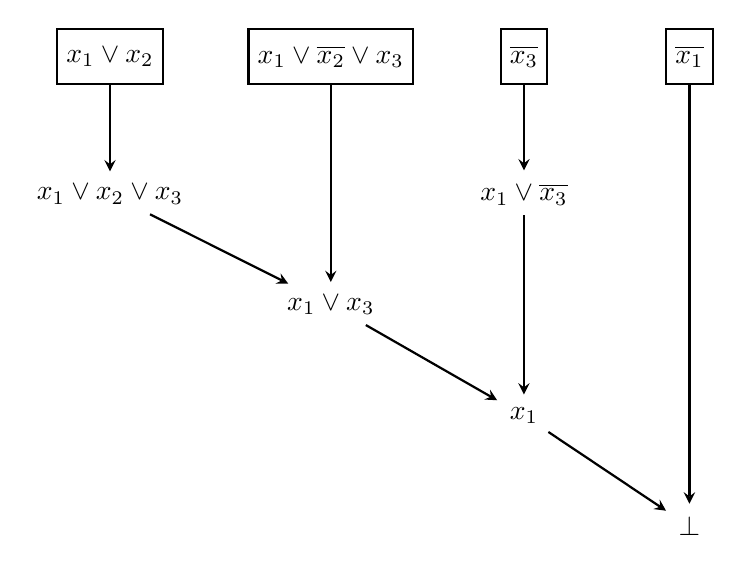
\begin{tikzpicture}[->,>=stealth,shorten >=1pt,auto,node distance=1.75cm, thick,main node/.style={scale=0.9,circle,draw,font=\sffamily\normalsize}]
            \node [rectangle, draw, minimum height=20](1) []{$x_1 \lor x_2$};
            \node [rectangle, draw, minimum height=20](2) [right of=1, xshift=30]{$x_1 \lor \overline{x_2} \lor x_3$};
            \node [rectangle, draw, minimum height=20](3) [right of=2, xshift=20]{$\overline{x_3}$};
            \node [rectangle, draw, minimum height=20](4) [right of=3, xshift=10]{$\overline{x_1}$};

            \node (5) [below of=1]{$x_1 \lor x_2 \lor x_3$};
            \node (6) [below of=2]{};
            \node (7) [below of=3]{$x_1 \lor \overline{x_3}$};
            \node (8) [below of=4]{};

            \node (9) [below of=2, yshift=-40]{$x_1 \lor x_3$};
            \node (10) [below of=3, yshift=-80]{$x_1$};
            \node (11) [below of=4, yshift=-120]{$\bot$};
        
            \path[every node/.style={font=\sffamily\small}]
                (1) edge (5)
                (2) edge (9)
                (5) edge (9)
                (3) edge (7)
                (4) edge (11)
                (9) edge (10)
                (7) edge (10)
                (10) edge (11)
                ;
        \end{tikzpicture}
        
        \caption{$\mathsf{TreeRes}$ refutation obtained from the $\mathsf{DTree}$ refutation of \Cref{dt_ref}.}
    \end{figure}

    Through a more precise argument, the weakening step can also be removed from the proof, giving us a tree-like resolution refutation that has size at most $s$ -- in fact, it may even have lower size if we \curlyquotes{skip} the excess queries.

    \begin{framedlem}{ $\mathsf{DTrees}$ p-simulates $\mathsf{TreeRes}$}
        Let $F$ be an unsatisfiable CNF formula. If $F$ has a tree-like resolution refutation of length $s$ and depth $d$, there is a decision tree refutation of length $s$ and depth $d$.
    \end{framedlem}

    \begin{proof}
        Let $T$ be a tree-like resolution refutation of length $s$ and depth $d$. W.l.o.g. we can assume that the weakening rule is never used inside this refutation. Let $F = C_1 \land \ldots \land C_m$.
        
        We procede by induction on the size $s$ of the refutation of $F$. If $s = 1$, then the refutation is made of only one step that ends with the empty clause, implying that $\exists j \in [m]$ such that $C_j = \bot$. Hence, the decision tree made of the single node labeled with $C_j$ is a refutation of $F$.

        Suppose now that the size $s$ of the refutation is bigger than 1. Let $x_i$ be the last variable resolved by the refutation, i.e. the one that yields $\bot$, and let $T_0$ and $T_1$ be the subtrees of $T$ such that $x_i$ is the root of $T_0$ and $\overline{x_i}$ is the root of $T_1$. Consider now the restricted formulas $F_{\mid x_i=0}$ and $F_{\mid x_i=1}$. It's easy to see that the subtrees $T_0$ and $T_1$ are refutations of these two formulas. Let $s_0$ and $s_1$ be the lengths of $T_0$ and $T_1$, where $s = s_0 + s_1 + 1$. By inductive hypothesis there are two decision trees $T'_0$ and $T'_1$ of size $s_0$ and $s_1$ that refute $F_{\mid x_i=0}$ and $F_{\mid x_i=1}$. We can build a new decision tree $T'$ that queries $x_i$ and proceedes on $T'_0$ when $x_i = 0$, otherwise it proceedes on $T'_1$. This new decision tree is clearly a refutation of $F$. Moreover, this new decision tree has size $s$ and depth $d$.
    \end{proof}


    \begin{figure}[H]
        \centering

        \resizebox{1\hsize}{!}{
            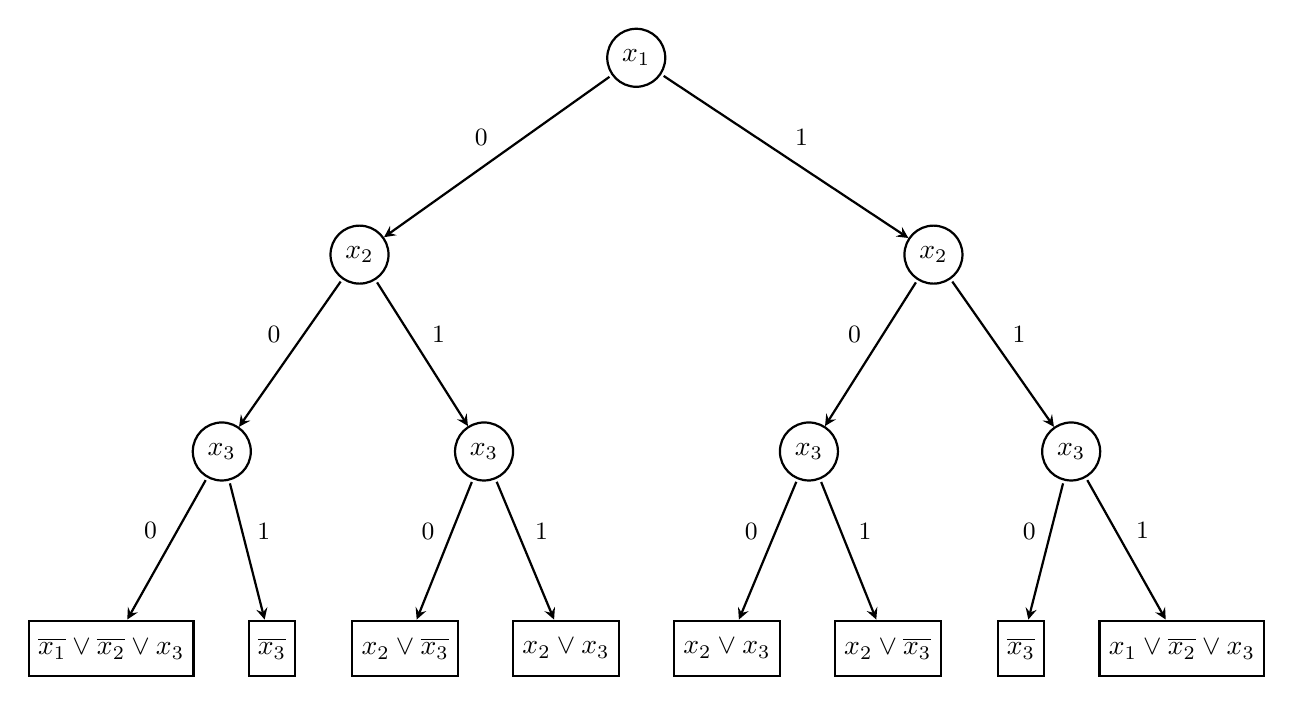
\begin{tikzpicture}[<-,>=stealth,shorten >=1pt,auto,node distance=2.5cm, thick,main node/.style={scale=0.9,circle,draw,font=\sffamily\normalsize}]
                \node [rectangle, draw, minimum height=20](1) []{$\overline{x_1} \lor \overline{x_2} \lor x_3$};
                \node [rectangle, draw, minimum height=20](2) [right of=1, xshift=-13]{$\overline{x_3}$};
                \node [rectangle, draw, minimum height=20](3) [right of=2, xshift=-23]{$x_2 \lor \overline{x_3}$};
                \node [rectangle, draw, minimum height=20](4) [right of=3, xshift=-13]{$x_2 \lor x_3$};
                \node [rectangle, draw, minimum height=20](5) [right of=4, xshift=-13]{$x_2 \lor x_3$};
                \node [rectangle, draw, minimum height=20](6) [right of=5, xshift=-13]{$x_2 \lor \overline{x_3}$};
                \node [rectangle, draw, minimum height=20](7) [right of=6, xshift=-23]{$\overline{x_3}$};
                \node [rectangle, draw, minimum height=20](8) [right of=7, xshift=-13]{$x_1 \lor \overline{x_2} \lor x_3$}; 

                \node[circle, draw] (9)[above of=1, xshift=40]{$x_3$};
                \node[circle, draw] (10)[above of=3, xshift=28.5]{$x_3$};
                \node[circle, draw] (11)[above of=6, xshift=-28.5]{$x_3$};
                \node[circle, draw] (12)[above of=8, xshift=-40]{$x_3$};

                \node[circle, draw] (13)[above of=10, xshift=-45]{$x_2$};
                \node[circle, draw] (14)[above of=11, xshift=45]{$x_2$};

                \node[circle, draw] (15)[above of=13, xshift=100]{$x_1$};
            
                \path[every node/.style={font=\sffamily\small}]
                    (1) edge node{$0$} (9)
                    (2) edge[swap] node{$1$} (9)
                    (3) edge node{$0$} (10)
                    (4) edge[swap] node{$1$} (10)
                    (5) edge node{$0$} (11)
                    (6) edge[swap] node{$1$} (11)
                    (7) edge node{$0$} (12)
                    (8) edge[swap] node{$1$} (12)

                    (9) edge node{$0$} (13)
                    (10) edge[swap] node{$1$} (13)
                    (11) edge node{$0$} (14)
                    (12) edge[swap] node{$1$} (14)

                    (13) edge node{$0$} (15)
                    (14) edge[swap] node{$1$} (15)
                    ;
            \end{tikzpicture}
        }
        
        \caption{$\mathsf{DTree}$ refutation obtained from the $\mathsf{TreeRes}$ refutation of \Cref{treelike_res_proof}.}
    \end{figure}

    \begin{framedthm}{$\mathsf{DTrees}$ p-equivalent to $\mathsf{TreeRes}$}
        $\mathsf{DTrees} \equiv_p \mathsf{TreeRes}$
    \end{framedthm}

    \section{The ordering principle}

    By definition, it clearly holds that $\mathsf{Res} \leq_p \mathsf{TreeRes}$ since any tree-like resolution refutation is also a dag-like resolution refutation. We also discussed how any tree-like refutation can be converted into a tree-like refutation. However, this new tree-like proof may have exponential size. This conversion process cannot be improved: there are some formulas that are \textit{easy} for resolution, meaning that polynomial length suffices, and \textit{hard} for tree-like resolution, meaning that they require exponential length. These formulas are called \textbf{separating} formulas.

    The formula that we'll use to prove that resolution is separated from tree-like resolution is the unsatisfiable CNF formula corresponding to the \textbf{ordering principle}. This principle expresses that given a order of a finite set of $n$ elements, there must always be a minimum element in the set for that order.
    
    To encode this principle as an unsatisfiable CNF formula, it's sufficient to encode each of the properties that define it. Given the set of $n$ elements, for each pair of elements $i,j \in [n]$ such that $i \neq j$ we define the variable $x_{i,j}$ such that $i < j$ if $x_{i,j} = 1$ and $i \geq j$ otherwise, for a total of $O(n^2)$ variables.

    Any order must satisfy the \textit{order axioms}, i.e. reflexivity, antisymmetry and transitivity. We can encode these axioms as follows:
    \begin{itemize}
        \item Since for each element $i \in [n]$ the variable $x_{i,i}$ doesn't exist, the reflexivity axiom is always satisfied.
        \item For each $i,j \in [n]$ with $i \neq j$, antisymmetry can be encoded as $\overline{x_{i,j} \land x_{j,i}}$, which can be rewritten as $\overline{x_{i,j}} \lor \overline{x_{j,i}}$
        \item For each $i,j,k \in [n]$ with $i \neq j, j \neq k$ and $k \neq i$, transitivity can be encoded as $x_{i,j} \land x_{j,k} \rightarrow x_{i,k}$, which can be rewritten as $\overline{x_{i,j}} \lor \overline{x_{j,k}} \lor x_{i,k}$
    \end{itemize}

    After encoding the conditions of an order, we now have to encode a contradiction to the ordering principle in order to get an unsatisfiable formula. Since the principle says that there must be a minimum element, the contradiction can be encoded by imposing a \textit{non-minimality axiom}: for each $i \in [n]$ there is always a $j \in [n]$ with $i \neq j$ such that $x_{j,i} = 1$. In other words, we're imposing that each element must have at least one predecessor.

    Finally, to obtain a CNF formula, the universal and existential quantification of each of these axioms can be expressed through a conjunction and disjuction over all the variables involved. 
    
    \begin{frameddefn}{Ordering principle}
        We define the \textbf{ordering principle} on $n$ elements $(\lnot\mathrm{OP}_n)$ as the following unsatisfiable CNF formula:
        \[\bigwedge_{\substack{i, j \in [n] :\\ i \neq j}} \overline{x_{i,j}} \lor \overline{x_{j,i}} \;\;\; \land \;\; \bigwedge_{\substack{i, j, k \in [n] :\\ i \neq j \\ j \neq k \\ k \neq i}} \overline{x_{i,j}} \lor \overline{x_{j,k}} \lor x_{i,k} \;\; \land \;\;\bigwedge_{i \in [n]} \bigvee_{\substack{j \in [n] :\\ i \neq j}} x_{j,i}\]

        The formula $\lnot \mathrm{OP}^n$ has $\Theta(n^3)$ clauses.
    \end{frameddefn}

    \textcite{stalmark} was able to show that this unsatisfiable CNF formula is easy for general resolution, i.e. that it has a small refutation in this proof system. In fact, the proof has linear size (remember than the formula contains $O(n^3)$ clauses). The idea behind the proof is to repeatedly reduce $\lnot\mathrm{OP}_n$ to $\lnot\mathrm{OP}_{n-1}$ until it reaches $\lnot\mathrm{OP}_2$, for which there is a known short refutation.
    
    \begin{framedthm}{}
        $\lnot\mathrm{OP}_n$ has a resolution refutation of length $O(n^3)$.
    \end{framedthm}

    \begin{proof}
        We'll use induction to prove the statement by reducing $\lnot\mathrm{OP}_n$ to $\lnot\mathrm{OP}_{n-1}$. When $n = 2$, the full formula corresponds to:
        \[\lnot\mathrm{OP}_2 \equiv (\overline{x_{1,2}} \lor \overline{x_{2,1}}) \land x_{1,2} \land x_{2,1}\]
        
        which can be proved by a refutation with less than $2^3$ clauses:
        \[\begin{array}{lcl}
            D_1 :& \overline{x_{1,2}} \lor \overline{x_{2,1}} & \text{Axiom} \\
            D_2 :& x_{1,2} & \text{Axiom} \\
            D_3 :& \overline{x_{2,1}} & \text{Res. on $D_1, D_2$} \\
            D_4 :& x_{2,1} & \text{Axiom} \\
            D_5 :& \bot & \text{Res. on $D_3, D_4$} \\
        \end{array}\]
        
        For the inductive hypothesis, we must be careful: the big-Oh notation imposes that there is a single constant $c$ such that $cn^3$ acts as an upper bound for each $n$ sufficiently big. In other words, the induction must be made on a single shared constant between each $n$. Thus, we must assume that $\lnot\mathrm{OP}_{n-1}$ has a refutation with $c(n-1)^3$ clauses. Otherwise, the different constants used may introduce some hidden exponential values.

        Before proceeding, we introduce some auxiliary notation:
        \begin{itemize}
            \item For any element $a \in [n]$ and a value $k \in [n]$, let $M_k(a)$ be the clause that represents the non-minimality of $a$ on the first $k$ variables, meaning that $M_k(a) = \bigvee_{\substack{j \in [k] :\\ a \neq j}} x_{j,a}$. 
            
            \item For any triple $a,b,c \in [n]$ where $a \neq b, b \neq c$ and $c \neq a$, let $T(a,b,c)$ be the clause that denotes the transitivity axiom on $a,b,c$, meaning that $T(a,b,c) = \overline{x_{a,b}} \lor \overline{x_{b,c}} \lor x_{a,c}$ 
        \end{itemize}

        We observe that $M_k(a) = M_{k-1}(a) \lor x_{k,a}$. Moreover, we also observe that for each $a \in [n]$ it holds that $M_n(a)$ is an axiom of $\lnot\mathrm{OP}_n$. Since $\lnot\mathrm{OP}_n$ already contains the antysimmetry and transitivity axioms of $\lnot\mathrm{OP}_{n-1}$, the idea behind the proof is to obtain $M_{n-1}(1), \ldots, M_{n-1}(n-1)$ in order to reduce $\lnot\mathrm{OP}_n$ to $\lnot\mathrm{OP}_{n-1}$.

        Fix an element $i \in [n]$. For each $j \in [n-1]$ such that $i \neq j$, we resolve $T(j,n,i)$ with $M_n(i)$ on the variable $x_{n,i}$ in order to obtain $M_{n-1}(i) \lor \overline{x_{j,n}}$ (notice that $x_{j,i}$ is already contained inside $M_{n-1}(i)$).
        \[\forall j \in [n-1], i \neq j \quad \frac{M_n(i) \quad T(j,n,i)}{M_{n-1}(i) \lor \overline{x_{j,n}}}\]

        With these $n-1$ resolution applications, we obtain the set of clauses $S_i = \{M_{n-1}(i) \lor \overline{x_{1,n}}, \ldots, M_{n-1}(i) \lor \overline{x_{n-1,n}}\}$. We observe that here the axiom $M_n(i)$ is being reused in each of these application without it being copied, making the proof non-tree-like.

        Consider now the axiom $M_n(n)$. Since this clause contains $x_{j,n}$ for each $j \in [n-1]$, we can repeatedly resolve this axiom on each clause of the set $S_i$ (using the previous resolvant for the next resolution) in order to obtain the clause $M_{n-1}(i)$, for a total of $n-1$ additional resolution steps. By also considering the axioms used, we get a total of $3n-1$ used clauses. If we reapeat this process for each $i \in [n-1]$, we can derive the clauses $M_{n-1}(1), \ldots, M_{n-1}(n-1)$ through $(3n-1)(n-1)$ clauses.

        By inductive hypothesis, $\lnot\mathrm{OP}_{n-1}$ has a proof of length at most $c(n-1)^3$. Hence, we get that $\lnot\mathrm{OP}_n$ has a proof of length at most $(3n-1)(n-1) + c(n-1)^3 \leq cn^3$ which is true for each $n \geq 1$ when $c \geq 3$.
    \end{proof}

    \begin{figure}[H]
        \centering

        \includegraphics[width=1\textwidth]{images/ord_res.pdf}

        \caption{Dag-like representation of how each $M_{n-1}(i)$ in the previous proof is derived}
    \end{figure}

    \section{The prover-delayer game}

    After proving that general resolution can efficiently refute the ordering principle, we'll now show that tree-like resolution strictly requires refutations of exponential length. This result was first proven by \textcite{tlres_lower}. Originally, there weren't any general techniques known for lower bounds of proof systems, in particular $\mathsf{TreeRes}$. In modern days, the standard method used for this proof system is the \textbf{prover-delayer game}, in particular the version of the game proposed by \textcite{prover_delayer}.

    The idea behind this game is similar to the concept of adversarial (or delayer) argument that we have already seen for decision trees: the prover wants to prove that the CNF $F$ is unsatisfiable, while the delayer tries to lag the prover's final answer as long as possible by keeping the formula still satisfiable by at least one extension of the current partial assignment known by the prover (the delayer will always eventually lose).

    \begin{frameddefn}{The prover-delayer game}
        Given an unsatisfiable CNF $F$, the \textbf{prover-delayer game} is a sequence of interactions between two entities, the prover and the delayer. On each interaction, the prover queries a variable $x_i$ defined in $F$, while the delayer has two options:
        \begin{enumerate}
            \item They answer with a value $b \in \{0,1\}$
            \item They let the prover answer with a value $b \in \{0,1\}$
        \end{enumerate}

        The delayer scores a \textbf{point} each time it lets the prover answer.
    \end{frameddefn}

    We notice that, by definition, only the delayer can score points. The delayer must try to score as many points as they can. The prover may query the same variable multiple times (the answer must be consistent with the previous ones).
 
    The idea behind how the scoring system of this game may seem counterintuitive: can't the delayer just let the prover answer each query and always get a point? The short answer is yes, but it's not guaranteed that this is the best option: there may be a sequence of queries that lets the prover decide the answer immediately. To counter this, the delayer's strategy must be as much adaptive as possible. Hence, each time answering with both 0 and 1 let's the game progress, the delayer lets the prover answer.
    
    Each of these situations corresponds to an \textbf{internal node} of any decision tree that the prover may be following to decide the answer. In other words, each time the delayer scores a point the game \textit{forks} into two possibilities that depend on the prover's answer. This implies that if the delayer can score $s$ points then there must be at least $2^s$ branches, each containing at least one leaf.

    \begin{framedthm}{The prover-delayer game method}
        Given an unsatisfiable CNF $F$, if the delayer can score at least $s$ points in the prover-delayer game then any decision tree that refutes $F$ must have at least $2^s$ leaves.
    \end{framedthm}

    \begin{proof}
        We'll prove an equivalent statement: if $F$ can be refuted by a decision tree with at most $k$ leaves then the delayer can win at most $\floor{\log k}$ points.

        Let $T$ be a decision tree that refutes $F$ with at most $\ell$ leaves and consider an arbitrary prover-delayer game on $F$ that uses this tree. Let $\alpha_i$ be the partial assignment constructed after $i$ rounds of the game and let $p_i$ be the number of points that the delayer has earned after $i$ rounds. Let $T_i$ be the sub-tree of $T$ which has as its root the node $v_i$ reached in $T$ along the path specified by $\alpha_i$, i.e. the subtree reached after $i$ rounds. For any sub-tree $T'$, let $\ell(T')$ be the number of leaves of $T'$. Let $m$ be the total number of rounds played by the game.
        
        \textbf{Claim}: For any $i \in [m]$, it holds that  $\ell(T_{i}) \leq \dfrac{\ell(T)}{2^{p_i}}$.

        \begin{proof}[Proof of the claim]
            We proceed by induction. At the beginning of the game we have that $p_0 = 0$ and $T_0 = T$, so the claim trivially holds. For the inductive step, assume that the claim holds for the first $i$ rounds. Let $x$ be the variable asked by the prover in the $(i+1)$-th round, i.e. the variable resolved at the root of the subtree $T_{i}$.
            
            If the delayer choses the answer, then $p_{i+1} = p_i$, making the statement hold by inductive hypothesis. Otherwise, the delayer gets a point, implying that $p_{i+1} = p_i +1$. Let $T_{i}^0$ and $T_i^1$ be the left and right sub-trees of $T_i$. Clearly, it holds that $\ell(T_i) = \ell(T_i^0) + \ell(T_i^1)$. Hence, one of the two sub-trees must have at most half the leaves of $T_i$. W.l.o.g. assume that $\ell(T_i^0) \leq \frac{\ell(T_i)}{2}$. By inductive hypothesis, we get that:
            \[\ell(T_i^0) \leq \frac{\ell(T_i)}{2} \leq \frac{\ell(T)}{2 \cdot 2^{p_i}} = \frac{\ell(T)}{2^{p_{i+1}}}\]
            concluding the proof.
        \end{proof}

        Since after the $m$-th round the subtree $T_m$ will correspond to an axiom clause, we know that $\ell(T_m) = 1$. Moreover, we also know that $\ell(T) = k$ by assumption. Hence, we get that:
        \[1 = \ell(T_m) \leq \frac{\ell(T)}{2^{p_m}} = \frac{k}{2^{p_m}}\]

        concluding that $p_m \leq \floor{\log k}$.
    \end{proof}

    The prover-delayer game makes proving lower bounds for refutation in decision trees and tree-like resolutions very easy: we have to just prove the existence of a strategy for the delayer that allows him to score a sufficient amount of points that impose an exponential lower bound on the proof complexity of the system.

    In particular, we'll show a strategy that allows the delayer to score at least $n-1$ points for the \textit{ordering principle}, giving an exponential lower bound for tree-like resolution. To be precise, we observe that since the number of clauses defined in $\lnot\mathrm{OP}_n$ is $m = \Theta(n^3)$, this lower bound is actually in the order of $2^{\Omega(\sqrt[3]{m})}$, which is still exponential.

    \begin{framedthm}{}
        Any $\mathsf{DTrees}$ and $\mathsf{TreeRes}$ refutation of $\lnot\mathrm{OP}_n$ has length at least $2^{n-1}$.
    \end{framedthm}

    \begin{proof}
        We'll show a delayer strategy that scores exactly $n-1$ points. The strategy is based on two data structures $H$ and $T$, called \textit{head} and \textit{tail}, used by the delayer as a mental picture of what the prover knows. $H$ is a set, while $T$ is an ordered list. The delayer will try to fool the prover as much as possible, making him think that each of the $k$ elements in the tail is part of a total order $i_1 < \ldots < i_k$, while every element in the head is a predecessor of the first element in $T$, i.e. $i_1$, which is referred to as the start of the tail.

        Initially, at the 0-th round, we have that $T = \varnothing$, $H = [n]$ and the delayer has not yet scored any point. Consider now a generic $i$-th round. Let $x_{i,j}$ be the variable queried by the prover. The answer of the delayer is given by four cases:
        \begin{enumerate}
            \item If both $i$ and $j$ are inside $T$, the delayer answers 1 if $i < j$ holds in the tail and 0 otherwise. In this case, the delayer simply replies with an information already known by the prover.
            \item If only $i$ is inside $T$, the delayer answers with 0. In this case, the delayer is trying to fool the prover into thinking that $j < i$.
            \item If only $j$ is inside $T$, the delayer answers with 1. In this case, the delayer is trying to fool the prover into thinking that $i < j$.
            \item If both $i$ and $j$ are inside $H$, the delayer lets the prover answer. This case gives the prover an undeniable answer, hence the delayer has to update the tail based on the answer given by the prover: if $x_{i,j} = 1$ then $j$ gets moved to the start of the tail, otherwise $i$ gets moved.
        \end{enumerate}

        As long as $T$ contains at most $n-2$ elements, after every round the number of points won by the delayer is equal to the number of elements in the tail and every axiom clause is still satisfiable. When $T$ contains exactly $n-1$ elements, instead, any possible assignment for any variable involving the last element inside $H$ will either falsify a transitivity axiom or a non-minimality axiom. Hence, when $T$ contains $n-1$ elements the prover can no longer be fooled and the formula will be declared unsatisfiable.
    \end{proof}

    \begin{figure}[H]
        \centering
        \begin{tabular}{r |c | l}
            Round & Status & Interaction \\
            \hline 
            1 & $\{1,2,3,4\}$ & $P: x_{1,3}? \to V: \text{you decide!} \to P: 1$ \\ 
            2 & $\{1,2,4\} < 3$ & $P: x_{2,3}? \to V: 1$ \\ 
            3 & $\{1,2,4\} < 3$ & $P: x_{1,4}? \to V: \text{you decide!} \to P: 0$ \\ 
            4 & $\{2,4\} < 1 < 3$ & $P: x_{4,1}? \to V: 1$ \\
            $\vdots$ & $\vdots$ & $\vdots$ \\
            $k$ & $\{2,4\} < 1 < 3$ & $P: x_{2,4}? \to V: \text{you decide!} \to P: 0$ \\
            $k+1$ & $\{4\} < 2 < 1 < 3$ & Non-minimality of $4$ falsified \\
        \end{tabular}

        \caption{Example of how the strategy may proceede for $\lnot\mathrm{OP}_4$}
    \end{figure}


    \section{The pigeonhole principle}

    We saw how general resolution is separaated from tree-like resolution because $\lnot\mathrm{OP}_n$ is easy for the former and hard for the latter. However, there are other basic formulas that are hard even for general resolution, such as the \textbf{Pigeohole principle}. This principle states that given two values $m > n$, it is not possible to fit $m$ pigeons into $n$ holes without at least two pigeons being assigned to the same hole. Mathematically, this corresponds to saying that any function from $m$ elements to $n$ elements cannot be \textit{injective}.

    To describe the pigeonhole principle for $m$ pigeons and $n$ holes as an unsatisfiable CNF, written as $\lnot\mathrm{PHP}_n^m$, for each $i \in [m]$ and each $j \in [n]$ we define the variable $x_{i,j}$ such that $x_{i,j} = 1$ if the $i$-th pigeon is assigned to the $j$-th hole. To encode the contradiction, we use the following axioms:
    \begin{itemize}
        \item \textit{Pigeon axioms}: every pigeon must have a hole assigned, i.e. $\forall i \in [m]$ we have the clause $\bigvee_{j \in [n]} x_{i,j}$
        \item \textit{Hole axioms}: no hole can contain have two pigeons assigned, i.e. $\forall j \in [n]$ we have the clauses $\bigwedge_{\substack{i, i' \in [m] :\\ i \neq i'}} \overline{x_{i,j}} \lor \overline{x_{i',j}}$
    \end{itemize} 

    \begin{frameddefn}{Pigeonhole principle}
        We define the \textbf{pigeonhole principle} on $m$ pigeons and $n$ holes elements where $m > n$ $(\lnot\mathrm{PHP}_n^m)$ as the following unsatisfiable CNF formula:
        \[\bigwedge_{i \in [m]} \bigvee_{j \in [n]} x_{i,j} \;\;\; \land \;\; \bigwedge_{j \in [n]}\bigwedge_{\substack{i, i' \in [m] :\\ i \neq i'}} \overline{x_{i,j}} \lor \overline{x_{i',j}}\]

        The formula $\lnot \mathrm{PHP}_n^m$ has $\Theta(nm^2)$ clauses.
    \end{frameddefn}

    Surprisingly, in almost any proof system the complexity of such formula depends only on the number of holes, even though $m > n$, meaning that we can have as many pigeons as we like. In tree-like resolution, an exponential lower bound is easily obtained through the prover-delayer game.

    \begin{framedthm}{}
        Any $\mathsf{DTrees}$ and $\mathsf{TreeRes}$ refutation of $\lnot\mathrm{PHP}_n^{n+1}$ has length at least $2^{n+1}$.
    \end{framedthm}

    \begin{proof}
        The mental image of the delayer corresponds to two simple initially empty sets $Y$ and $N$ of pairs $(i,j)$, where $i$ is the index of a pigeon and $j$ is the index of a hole. The first sets will contain the mappings known to be true by the prover, while the latter will contain the mapps that are known to be false. When the prover queries the variable $x_{i,j}$, the delayer answers with the following strategy:
        \begin{itemize}
            \item If $(i,j) \in N$, the delayer answers with 0.
            \item If $(i,j) \in Y$, the delayer answers with 1.
            \item If $(i,b) \in Y$ with $b \neq j$, the delayer answers with 0
            \item If $(a,j) \in Y$ with $a \neq i$, the delayer answers with 0
            \item If $\forall (a,b) \in Y$ it holds that $i \neq a$ and $j \neq b$, the delayer lets the prover answer. If the answer is 1, the delayer adds the pair $(i,j)$ to the set $Y$. If the answer is 0, the delayer adds the pair $(i,j)$ to the set $N$.
        \end{itemize}
    
        The invariant that holds in this case is that the number of points scored by the delayer is always at least equal to the number of pairs in $Y$. When $\abs{Y} = n+1$, at least one axiom is falsified, concluding the game.
    \end{proof}

    \newpage

    We observe that this lower bound is not perfect. \textcite{php_treeres} proved that there is a more thigh bound on the size complexity of $\lnot\mathrm{PHP}_n^m$: the proof complexity in $\mathsf{DTrees}$ and $\mathsf{TreeRes}$ of $\lnot\mathrm{PHP}_n^m$ is actually $2^{\Theta(n \log n)}$. This shows that the pigeonhole principle is even harder than the ordering principle for tree-like resolution. 

    However, the pigeonhole principle is not only hard for tree-like resolution but also for general resolution, even though it performs slightly better than the tree-like system. We prove this result through the \textbf{bottleneck technique}, first defined by \textcite{haken} and later improved by \textcite{beame_pitassi}.

    The key observation behind this proof is that it suffices to show that $\lnot\mathrm{PHP}_n^{n+1}$ requires exponential length proofs in resolution since $\lnot\mathrm{PHP}_n^m$ for any $m > n+1$ includes $\lnot\mathrm{PHP}_n^{n+1}$ as a subformula.

    The technique is based on two concepts: \textit{critical assignments} and \textit{fat clauses}. Any variable assignment for $\lnot\mathrm{PHP}_n^m$ can be graphically described as an $m \times n$ matrix whose entries correspond to the variables $x_{i,j}$. In order for an assignment to satisfy $\lnot\mathrm{PHP}_n^m$, every row -- corresponding to a pigeon -- in the assignment must have at least one entry set to 1, while every column -- corresponding to a hole -- must have at most one entry set to 1. Since the formula is unsatisfiable, no assignment matrix can have the satisfying property.

    \begin{figure}[H]
        \centering

        \begin{tabular}{c c c}
            \begin{tabular}{|c|c|c|c|}
                \hline
                1 & 0 & 0 & 0 \\
                0 & 1 & 0 & 0 \\
                0 & 0 & 1 & 0 \\
                0 & 0 & 0 & 1 \\
                1 & 0 & 0 & 0 \\
                \hline
            \end{tabular}

            & \qquad\qquad &
            
            \begin{tabular}{|c|c|c|c|}
                \hline
                1 & 0 & 0 & 0 \\
                0 & 0 & 1 & 0 \\
                0 & 0 & 0 & 0 \\
                0 & 1 & 0 & 0 \\
                0 & 0 & 0 & 1 \\
                \hline
            \end{tabular}
        \end{tabular}

        \caption{Two assignments for $\lnot \mathrm{PHP}_4^5$}
        \label{assign_php}
    \end{figure}

    We now restrict our interest to $\lnot \mathrm{PHP}^{n+1}_n$. We say that an assignment $\alpha$ is \textit{$i$-critical} for $\lnot \mathrm{PHP}^{n+1}_n$ if the $i$-th row inside $M_\alpha$ is the only 0-row and every column has exactly one entry set to 1. In other words, an $i$-critical assignment is an injective mapping of $n$ pigeons to $n$ holes, where only the $i$-th pigeon is not mapped. For example, the right matrix shown in \Cref{assign_php} is $3$-critical. We say that $\alpha$ is \textit{critical} if it is $i$-critical for some $i \in [n+1]$. 

    Restricting attention to these assignments simplifies notation since it allows us to make every clause in the refutation \textit{monotone}, i.e. a clause with no occurence of negated variables. These monotone clauses will be satisfied by the same critical assignments of the original clauses. To get the monotone clause $C^+$ from the clause $C$, we convert any occurrence of the negated variable $\overline{x_{i,j}}$ with the disjuction over all the variables in the $j$-th column, except $x_{i,j}$.
    \[\overline{x_{i,j}} \mapsto x_{1,j} \lor \ldots \lor x_{i-1,j} \lor x_{i+1,j} \lor \ldots x_{n+1,j}\] 

    We notice that the monotone version of every hole axiom $\overline{x_{i,j}} \lor \overline{x_{i',j}}$ corresponds to the disjunction of all the variables in the $j$-th column, hence it is always satisfied by any critical assignment. Furthermore, for any critical assignment $\alpha$ it's easy to see that $C(\alpha) = C^+(\alpha)$. By way of contradiction, suppose there is a critical assignment $\beta$ such that $C(\beta) \neq C^+(\beta)$. This could only happen if $C$ contains a literal $\overline{x_{i,j}}$ such that $\overline{x_{i,j}} \neq \bigvee_{\substack{i' \in [n+1] \\ i \neq i'}} x_{i',j}$, but this is impossible since $\alpha$ has precisely one 1 in the $j$-th column.

    \begin{framedlem}{}
        Every \textsf{Res} refutation of $\lnot \mathrm{PHP}_n^{n+1}$ has a clause $C$ with $\mathrm{width}(C^+)\geq \frac{(n+1)^2}{9}$

        \textit{Note}: recall that the width of a clause is the number of literals inside it
    \end{framedlem}

    \begin{proof}
        Given a refutation $R$ of $\lnot \mathrm{PHP}_n^{n+1}$, for each clause $C$ inside $R$ we define $\mathrm{Pigeon}(C)$ as the set of pigeons that are \curlyquotes{bad} for $C$, i.e. those that have a critical assignment that falsifies $C$
        \[\mathrm{Pigeon}(C) = \{i \in [n+1] \mid \exists \alpha \text{ $i$-critical assignment s.t. } C(\alpha) = 0\}\]
        We define the \textit{significance} of a clause, denoted $\sigma(C)$, as the number of such bad pigeons, meaning that $\sigma(C) = \abs{\mathrm{Pigeon}(C)}$. By the definition, each pigeon axiom has significance 1, each hole axiom has significance 0 and the final empty clause of the refutation has significance $n+1$ since it is falsified by any assignment. 

        \textbf{Claim 1}: the significance of a clause is sub-additive under resolution, meaning that if $C$ is derived from $A$ and $B$ then $\sigma(C) \leq \sigma(A) + \sigma(B)$.

        \begin{proof}[Proof of the claim]
            By definition of the resolution itself, every assignment (even a non-critical one) satisfying $A$ and $B$ must also satisfy $C$. Hence, by contrapositive, if an assignment falsifies $C$ then it must also falsify $A$ or $B$.
        \end{proof}

        Since the axioms have significance at most 1, the empty clause has signficance $n+1$ and the significance is sub-additive, there must be a clause $D$ such that $\frac{1}{3} (n+1) \leq \sigma(D) \leq \frac{2}{3}(n+1)$ through an argument similar to the one of the \nameref{13_23_lemma}.

        \textbf{Claim 2}: $\mathrm{width}(D^+) \geq \sigma(D)(n+1-\sigma(D))$.

        \begin{proof}[Proof of the claim]
            Fix $i \in \mathrm{Pigeon}(D)$ and let $\alpha$ be an $i$-critical assignment that falsifies $D$. For each $i' \in [n+1] - \mathrm{Pigeon}(D)$, we construct an $i'$-critical assignment $\alpha'$ obtained from $\alpha$ by swapping the rows $i$ and $i'$. Since $i' \notin \mathrm{Pigeon}(D)$, we know that $D(\alpha') = 1$.
            
            Hence, since $D(\alpha) = D^+(\alpha)$ and $D(\alpha') = D^+(\alpha')$, we know that $D^+(\alpha) = 0$ and $D^+(\alpha') = 1$. Since the assignments $\alpha, \alpha'$ differ only in the variables $x_{i,j}$ and $x_{i',j}$, in order for $D^+(\alpha) = 0$ and $D^+(\alpha') = 1$ to holds we have that $D^+$ contains the variable $x_{i',j}$. By repeating this argument on each $i \in \mathrm{Pigeon}(D)$ and each $i' \in [n+1] - \mathrm{Pigeon}(D)$, we get that $D^+$ must contain at least $\sigma(D)(n+1-\sigma(D))$ variables.
        \end{proof}

        Since $\frac{1}{3} (n+1)\leq \sigma(D) \leq \frac{2}{3} (n+1)$, the previous claim concludes the proof.
    \end{proof}

    \newpage

    \begin{framedthm}{Haken-Beame-Pitassi theorem}
        Any $\mathsf{Res}$ refutation of $\lnot\mathrm{PHP}_n^{n+1}$ has length $2^{\Omega(n)}$.
    \end{framedthm}

    \begin{proof}
        Let $R$ be a resolution refutation proof of $\lnot \mathrm{PHP}_n^{n+1}$
        Let $a,b \geq 2$ be two positive values -- we'll specify their value lated in the proof in order to not make them look like magic values. By way of contradiction, assume that the length of $R$ is less than $e^{\frac{n}{a}}$. Let $R^+ = \{C^+ \mid C \in R\}$ be the monotonized set of clauses obtained from $R$. We say that a clause $C$ is \textit{fat} if $\mathrm{width}(C) \geq \frac{(n+1)^2}{b}$. Let $\gamma$ be the number of fat clauses in $R^+$. Since each fat clause has at least a $\frac{1}{b}$ fraction of all the variables ($\lnot \mathrm{PHP}^{n+1}_n$ has $n(n+1)$ variables), there must be (ironically, by the pigeonhole principle) a variable $x_{i,j}$ that occurrs in at least $\frac{\gamma}{b}$ fat clauses in $R^+$.

        We'll now construct a partial assignment $\alpha$ that will be used to restrict the formula. Inside $\alpha$, we set $x_{i,j} = 1$ and also set $x_{i',j} = 0$ and $x_{i,j'} = 0$ for each $i' \neq i$ and each $j' \neq j$ (we're setting the whole row and the whole column containing $x_{i,j}$ to 0, while $x_{i,j}$ is set to 1). This assignment affirms that the $i$-th pigeon is mapped to only the $j$-th hole and that the $j$-th contains only the $i$-th pigeon.
        
        Furthermore, we notice that this assignment sets to 1 every single fat monotone clause in $R^+$ that contains $x_{i,j}$, while all the other variables that are set to 0 in $\alpha$ will disappear from the remaining clauses. By applying the restriction on $\alpha$ the whole refutation $R$, we get a refutation $R_1$ for $\lnot \mathrm{PHP}_{n-1}^{n}$ (up to renaming the indices), where the number of fat clauses in $R_1^+$ is at most $\gamma - \frac{\gamma}{b} = \gamma\rbk{1-\frac{1}{b}}$. By applying this procedure iteratively for $d = b \ln \gamma$ times, we're guaranteed to have removed all the fat clauses since:
        \[\gamma\rbk{1-\frac{1}{b}}^d = e^{\ln\rbk{\gamma\rbk{1-\frac{1}{b}}^d}} < e^{\ln \gamma - \frac{d}{b}} = 1\]

        Thus, we're left with a refutation $R_d$ of $\lnot \mathrm{PHP}_{n-d}^{n+1-d}$, where $\mathrm{width}(C^+) < \frac{(n+1)^2}{b}$ for all the clauses $C$ of the refutation (due to the restriction process). However, by the previous lemma, we know that this refutation must have a clause $D$ such that $\mathrm{width}(D^+) \geq \frac{(n+1-d)^2}{9}$. Since it also holds that $d = b \ln \gamma < b \ln(e^{\frac{n}{a}}) = \frac{bn}{a}$, we get that:
        \[\frac{(n+1)^2}{b} > \mathrm{width}(D^+) \geq \frac{(n+1-d)^2}{9} \geq \frac{\rbk{1-\frac{b}{a}}^2n^2}{9}\]

        To get a contradiction, it is enough to chose two values $a,b$ for which $\rbk{1-\frac{b}{a}}^2 \geq \frac{9}{b}$ holds. In particular, the values $a = 2$ and $b = 9$ suffice. Thus, we get that there cannot exist a resolution refutation for $\mathrm{PHP}_{n}^{n+1}$ that has length less than $e^{\frac{n}{2}}$        
    \end{proof}

    We notice that, exception made for the lemma, in this proof we never used the fact that the clauses in a refutation are derived using only resolution and weakening rules. In fact, the same argument also works for other proof systems that are capable of satisfying the sub-additivity of sensitivity. Except this, the only important thing was that the formulas in such a derivation are clauses, which allowed us to kill off clauses by setting just one variable to a constant. 

    \newpage

    \section{Cutting planes}

    We now turn our attention to a more powerful proof system based on geometric arguments, the \textbf{cutting planes} ($\mathsf{CP}$) proof system. The cutting planes method originated in works on integer programming by \textcite{gomory_cutting, chvatal_cutting}; as a proof system it was first considered by \textcite{cook_cutting}. The basic idea is to use a few elementary geometrical rules (based on linear algebra) to prove that a given system of linear inequalities with integer coefficients does not have a 0-1 solution.

    Let $A$ be a matrix with integer entries and let $b$ be an integer vector. We are interested in boolean-valued solutions to the system of inequalities $Ax \leq b$ (over integer arithmetic).

    \begin{figure}[H]
        \centering

        \begin{tabular}{ccc}
            $\begin{array}{c c c}
                a_{1,1}x_1 + \ldots + a_{1,n}x_n &\leq& b_1 \\
                \vdots & & \vdots\\
                a_{m,1}x_1 + \ldots + a_{m,n}x_n &\leq& b_m \\
            \end{array}$

            &\quad$\longleftrightarrow$\qquad\quad&

            $\smat{
                a_{1,1} & \cdots & a_{1,n} \\ 
                \vdots & \ddots & \vdots \\
                a_{m,1} & \cdots & a_{m,n} \\ 
            } \smat{x_1 \\ \vdots \\ x_n} \leq \smat{b_1 \\ \vdots \\ b_m}$
        \end{tabular}
        
        \caption{The system of linear inequalities (left) and the matricial inequality (right) are equivalent}
    \end{figure}
    
    In the context of 0-1 integer programs, we say that the system $Ax \leq b$ is unsatisfiable if there is no $x \in \{0,1\}^n$ that is a solution of the system. Such unsatisfiable systems are our objects of interest for the cutting plane proof systems, taking the place of the unsatisfiable CNFs formulas studied in resolution. In other words, given an unsatisfiable system of inequalities, our goal is to prove its unsatisfiability using repeated applications of the system's rules. The cutting planes proof system consists of three rules of derivation:
    \begin{enumerate}
        \item \textbf{Addition of inequalities}: if $a_1^T x \leq b_1$ and $a_2^T x \leq b_2$ are two inequalities of the system then we can derive the inequality $(a_1+a_2)^T x \leq b_1 + b_2$.
        \[\frac{a_1^T x \leq b_1 \qquad a_2^T x \leq b_2}{(a_1+a_2)^T x \leq b_1 + b_2}\]

        \item \textbf{Multiplication by scalar}: if $a^T x \leq b$ is an inequality of the system then for any $k \in \Z_{> 0}$ we can derive the inequality $k a^T x \leq kb$.
        \[\forall k \in \Z_{> 0} \qquad \frac{a^T x \leq b}{k a^T x \leq kb}\]

        \item \textbf{Gomory-Chvátal cut} (or \textit{rounded division}): if $k a^T x \leq b$ for some $k \in \Z_{> 0}$ is an inequality of the system then we can derive the inequality $k a^T x \leq b$.
        \[\forall k \in \Z_{> 0} \qquad \frac{k a^T x \leq b}{a^T x \leq \floor{\frac{b}{k}}}\]

    \end{enumerate}
    
    The correctness of the first two rules come from simple linear algebra properties. The third rule, instead, comes from the fact that if the coefficients $a_1, \ldots, a_n$ are all multiples of an integer $d$ then any integer solution of $a_1 x_1 + \ldots + a_n x_n \leq b$ is also a solution of $\frac{a_1}{d} x_1 + \ldots + \frac{a_n}{d} x_n \leq \floor{\frac{b}{d}}$. This result is the real power of the cutting planes proof system; it can be used to simplify inequalities of the system without killing off possible solutions.
    
    \begin{figure}[H]
        \centering

        \includegraphics[scale=0.5]{images/cutplane.png}
        \caption{A cutting plane derivation of $x \leq 1$ from the initial inequalities $x - y \leq 1$ and $x+y \leq 2$. The first image corresponds to the initial feasible region (the black dots are the integer solutions). The second image is obtained by applying the addition rule on the two inequalities, deriving $2x \leq 3$. The third image is obtained by applying the cut rule on $2x \leq 3$, obtaining $x \leq 1$.}
    \end{figure}
    
    If through the repeated application of these rules we're able to derive the inequality $0 \leq -1$ (which is clearly unsatisfiable) from the initial system of inequalities, then the latter must also be unsatisfiable.
    
    \begin{frameddefn}{Cutting planes refutation}
        Given a system of inequalities $\Phi$, a \textbf{cutting planes refutation} of $\Phi$ is a sequence of inequalities $\phi_1, \ldots, \phi_k$ such that the last inequaity is $0^T x \leq -1$ and for each $i$ one of the following holds:
        \begin{itemize}
            \item $d_i^T x \leq q_i$ is one of the axioms of $\Phi$, i.e. one of it's initial inequalities
            \item $d_i^T x \leq q_i$ is the addition of $\phi_j$ with $\phi_h$, where $j,h < i$
            \item $d_i^T x \leq q_i$ is a multiplication by scalar of $\phi_j$, where $j < i$ 
            \item $d_i^T x \leq q_i$ is a Gomory-Chvátal cut of $\phi_j$ where $j < i$
        \end{itemize}
    \end{frameddefn}


    For example, given the following system of linear inequalities:
    \[\begin{array}{rcl}
        -y+z & \leq & 0 \\
        -x+y & \leq & 0 \\
        y & \leq &1 \\
        x-z & \leq &0 \\
        x+y+z & \leq &2 \\
        -x-y-z & \leq &-1 \\
    \end{array}\]

    a cutting planes refutation for $F$ is given by:
    \[\begin{array}{lcl}
        \phi_1 :& y \leq 1 & \text{Axiom} \\
        \phi_2 :& x-z \leq 0  & \text{Axiom} \\
        \phi_3 :& x+y-z \leq 1  & \text{Sum of $\phi_2, \phi_3$} \\
        \phi_4 :& x+y+z \leq 2  & \text{Axiom} \\
        \phi_5 :& 2x+2y \leq 3  & \text{Sum of $\phi_3,\phi_4$} \\
        \phi_6 :& x+y \leq 1  & \text{Cut of $\phi_5$ by 2} \\
        \phi_7 :& -x+y \leq 0  & \text{Axiom} \\
        \phi_8 :& 2y \leq 1  & \text{Sum of $\phi_6, \phi_7$} \\
        \phi_9 :& y \leq 0  & \text{Cut of $\phi_8$ by 2} \\
        \phi_{10} :& -y+z \leq 0  & \text{Axiom} \\
        \phi_{11} :& z \leq 0  & \text{Sum of $\phi_9, \phi_{10}$} \\
        \phi_{12} :& x \leq 0  & \text{Sum of $\phi_{2}, \phi_{11}$} \\
        \phi_{13} :& -x-y-z \leq -1  & \text{Axiom} \\
        \phi_{14} :& -x-z \leq -1  & \text{Sum of $\phi_9, \phi_{13}$} \\
        \phi_{15} :& -x \leq -1 & \text{Sum of $\phi_{11}, \phi_{14}$} \\
        \phi_{16} :& 0 \leq -1 & \text{Sum of $\phi_{12}, \phi_{15}$} \\
    \end{array}\]

    Just like resolution, cutting planes refutations can also be represented through a directed acyclic graph.

    \begin{figure}[H]
        \centering
        \includegraphics[width=1\textwidth]{images/cutplanes_ref.pdf}
        
        \caption{Dag-like representation of the previous refutation.}
    \end{figure}

    \newpage

    When the underlying graph of a cutting planes refutation assumes the form of a tree, just like in resolution, we say that the refutation is tree-like. The restricted cutting planes proof system where the refutations must be tree-like is called \textbf{tree-like cutting planes} ($\mathsf{TreeCP}$). 

    The soundness of this proof system is guaranteed by the correctness of the cut rule: if the system has a feasible solution, the cut rule never kills it. Hence, if the system is satisfiable, there is no cutting planes refutation. The completeness, instead, comes from \textbf{Farkas' lemma}, which states that given a matrix $A \in \R^{m \times n}$ and a $b \in \R^m$ exactly one of the two always holds:
    \begin{itemize}
        \item There is an $x \in \R^n$ such that $A x \leq b$ and $x \geq 0$
        \item There is an $y \in \R^n$ such that $A^T y \geq 0$ and $y \geq 0$ with $b^T y < 0$
    \end{itemize}

    Farkas' lemma has also other applications in complexity theory. For example, it implies that the decision problem \curlyquotes{given a system of linear equations, does it have a non-negative solution?} lies in $\mathsf{NP} \cap \mathsf{coNP}$. This is because, according to the lemma, both a \curlyquotes{yes} answer and a \curlyquotes{no} answer have a proof that can be verified in polynomial time.

    While cutting plane proofs apply to linear systems, not CNFs, it is not difficult to \curlyquotes{translate} CNFs into equivalent linear systems. This translation can be achieved through the same process that we used in \Cref{01_prog} to show that $\mathrm{0/1\text{-}PROG}$ is $\mathsf{NP}$-Complete by reducing $\mathsf{CNF}\text{-}\mathsf{SAT}$ to it. For example, the CNF $F = (x_1 \lor x_2) \land (x_1 \lor \overline{x_2}) \land (\overline{x_1} \lor x_2) \land (\overline{x_1} \lor \overline{x_2})$ gets translated to the following system:
    \[\begin{array}{rcl}
        x_1 + x_2 & \geq & 1 \\
        x_1 + (1-x_2) & \geq & 1 \\
        (1-x_1) + x_2 & \geq & 1 \\
        (1-x_1) + (1-x_2) & \geq & 1 \\
    \end{array}\]

    After this translation process, we can move every constant value from the left side of each inequality to its right left. Finally, we can flip the sign of the inequality, obtaining the following standard system.
    \[\begin{array}{rcl}
        -x_1 - x_2 & \leq & -1 \\
        -x_1 + x_2 & \leq & 0 \\
        x_1 + x_2 & \leq & 0 \\
        x_1 + x_2 & \leq & 1 \\
    \end{array}\]

    Hence, in a more immediate way, each clause $C_j$ of a CNF $F$ is mapped to the inequality $\sum_{i \in [n]} a_{j,i} x_i \leq m-1$ where $m$ is the number of negated variables in $C_j$ and:
    \[a_{j,i} = \soe{cl}{
        -1 & \text{if } x_i \in C_j \\
        1 & \text{if } \overline{x_i} \in C_j \\
        0 & \text{otherwise}
    }\]

    Thus, we can study the length of refutations of CNFs in the cutting planes system and compare this to their refutation length under resolution. In particular, any resolution refutation can be be translated into cutting plane refutations in a very natural way by simply doubling the length of the proof, implying that cutting planes $p$-simulates resolution (and through the same argument that tree-like cutting planes $p$-simulates tree-like resolution).

    \begin{framedthm}{$\mathsf{CP}$ $p$-simulates $\mathsf{Res}$}
        $\mathsf{CP} \leq_p \mathsf{Res}$ and $\mathsf{TreeCP} \leq_p \mathsf{TreeRes}$
    \end{framedthm}

    \begin{proof}
        Let $R$ be a resolution refutation. W.l.o.g. we assume that the weakening rule is never used in this refutation. We'll show that any resolution step can be simulated through an addition rule followed by a cut.

        We proceed by structural induction on the refutation. For any clause $C$ in $R$, let $\sum_{i \in [n]} a_{i} x_i \leq m-1$ be the traslation of $C$, where $m$ is the number of negated variables in $C$. Let $f = \sum_{i \in [n]} a_{i} x_i$. If $C$ is an axiom then $f \leq m-1$ is also an axiom of any (tree-like) cutting-planes refutation. Suppose now that $C$ is derived from the clauses $C \lor x_{i}$ and $C \lor \overline{x_i}$. These two clauses correspond to the inequalities $f - x_i \leq m-1$ and $f + x_i \leq m$. By inductive hypothesis, suppose that we have already derived these two inequalities in the cutting planes proof. By first applying the addition rule and then the cut rule, we can derive the inequality corresponding to $C$:
        \[\dfrac{f - x_i \leq m-1 \qquad f + x_i \leq m}{2f \leq 2m-1} \quad \longrightarrow \quad \dfrac{2f \leq 2m-1}{f \leq m-1}\]

         Since each resolution step is mapped to two cutting planes step, the length of the proof is at most doubled. If $R$ is tree-like, the cutting planes proof is also tree-like.
    \end{proof}

    Although restricted, tree-like CP proofs are still very powerful. For example, we already know that the CNF formula $\lnot\mathrm{PHP}^{m}_n$ has no resolution proof of polynomial size. On the other hand, this CNF has relatively short proofs in $\mathsf{TreeCP}$ (and even shorter ones in $\mathsf{CP}$). This result separates $\mathsf{TreeCP}$ from $\mathsf{TreeRes}$ (and $\mathsf{CP}$ from $\mathsf{Res}$).

    \begin{framedthm}{}
        For any $m > n$, $\lnot \mathrm{PHP}_n^m$ has a tree-like cutting planes refutation of length $O(nm^2)$
    \end{framedthm}

    \begin{proof}
        When translated to the language of inequalities, the axioms for the pigeonhole principle consist of the following inequalities.
        \begin{itemize}
            \item Pigeon axioms: for each $i \in [m]$ we have the inequality $-x_{i,1} - \ldots - x_{i,n} \leq -1$
            \item Hole axioms: for each $j \in [n]$ and each $i, i' \in [m]$ where $i \neq i'$ we have the inequality $x_{i,j} + x_{i',j} \leq 1$
        \end{itemize}
        
        The idea behind the proof is to inductively derive $x_{1,j} + \ldots + x_{m,j} \leq 1$ for each hole $j \in [n]$ starting from $x_{1,j} + x_{2,j} \leq 1$, which is a hole axioms.
        
        Fix $j \in [n]$ and suppose that we have already derived $x_{1,j} + \ldots + x_{k,j} \leq 1$ through at most $ck^2$ clauses for some $c > 0$. First, we multiply the inequality by $k-1$ and then subsequently add to the result the hole axiom $x_{i,j} + x_{k+1, j} \leq 1$ for each $i \in [k]$, obtaining the following inequality.
        \[kx_{1,j} + \ldots + kx_{k+1,j} \leq 2k-1\]

        Finally, through the cut rule, we get the inequality $x_{1,j} + \ldots + x_{k+1,j} \leq 1$. The total number of clauses, assuming the used axioms are duplicated in order to make the proof tree-like, needed to derive this inequality are at most $3+2k$. By summing the at most $ck^2$ clauses needed to derive $x_{1,j} + \ldots + x_{k,j} \leq 1$, we have $3+2k+ck^2$ clauses, which is at most equal to $c(k+1)^2$ when $c \geq 3$, concluding the inductive step. Hence, we can derive each $x_{1,j} + \ldots + x_{m,j} \leq 1$ over all $j \in [n]$ through a total of at most $cnm^2$ clauses.

        Now, we sum these inequalities $x_{1,j} + \ldots + x_{m,j} \leq 1$ together over all $j \in [n]$ in order to obtain the inequality $\sum_{i \in [m], j \in [n]} x_{i,j} \leq n$. This requires $n-1$ additional clauses. On the other hand, by summing all the pigeon axioms together over all $i \in [m]$, we obtain the inequality of the form $-\sum_{i \in [m], j \in [n]} x_{i,j} \leq -m$. This requires $m-1$ additional clauses.
        
        Finally, by summing these two inequalities, we get $0 \leq n-m$. Since by assumption $m > n$, by dividing this last inequality by $\abs{n-m}$ we get the contradiction $0 \leq -1$. The total number of clauses used in this tree-like proof is at most $cnm^2+n+m = O(nm^2)$.
    \end{proof}

    We observe that the size of this proof has polynomial size, but its depth is $\Omega(n)$. There are known ways to balance this proof while maintaining the size polynomial, reducing the depth up to $O(\log n)$. \textcite{rhodes} showed that this cannot be improved: any cutting planes proof for $\lnot \mathrm{PHP}_n^m$ has depth $\Omega(\log n)$.

    Of course, the cutting planes proof system has some downsides. \textcite{cp_lower} was able to prove exponential lower bounds for cutting planes through a technique called \textit{feasible interpolation}. Moreover, \textcite{cp_autom} proved that \textit{automating} cutting planes is $\mathsf{NP}$-Hard.

    
\addcontentsline{toc}{chapter}{Bibliography}  % Add Bibliography to ToC
\printbibliography

\end{document}
